\documentclass[twoside]{book}

% Packages required by doxygen
\usepackage{fixltx2e}
\usepackage{calc}
\usepackage{doxygen}
\usepackage{graphicx}
\usepackage[utf8]{inputenc}
\usepackage{makeidx}
\usepackage{multicol}
\usepackage{multirow}
\PassOptionsToPackage{warn}{textcomp}
\usepackage{textcomp}
\usepackage[nointegrals]{wasysym}
\usepackage[table]{xcolor}
\usepackage{ifpdf,ifxetex}

% Font selection
\usepackage[T1]{fontenc}
\usepackage[scaled=.90]{helvet}
\usepackage{courier}
\usepackage{amssymb}
\usepackage{sectsty}
\renewcommand{\familydefault}{\sfdefault}
\allsectionsfont{%
  \fontseries{bc}\selectfont%
  \color{darkgray}%
}
\renewcommand{\DoxyLabelFont}{%
  \fontseries{bc}\selectfont%
  \color{darkgray}%
}
\newcommand{\+}{\discretionary{\mbox{\scriptsize$\hookleftarrow$}}{}{}}

% Page & text layout
\usepackage{geometry}
\geometry{%
  a4paper,%
  top=2.5cm,%
  bottom=2.5cm,%
  left=2.5cm,%
  right=2.5cm%
}
\tolerance=750
\hfuzz=15pt
\hbadness=750
\setlength{\emergencystretch}{15pt}
\setlength{\parindent}{0cm}
\setlength{\parskip}{3ex plus 2ex minus 2ex}
\makeatletter
\renewcommand{\paragraph}{%
  \@startsection{paragraph}{4}{0ex}{-1.0ex}{1.0ex}{%
    \normalfont\normalsize\bfseries\SS@parafont%
  }%
}
\renewcommand{\subparagraph}{%
  \@startsection{subparagraph}{5}{0ex}{-1.0ex}{1.0ex}{%
    \normalfont\normalsize\bfseries\SS@subparafont%
  }%
}
\makeatother

% Headers & footers
\usepackage{fancyhdr}
\pagestyle{fancyplain}
\fancyhead[LE]{\fancyplain{}{\bfseries\thepage}}
\fancyhead[CE]{\fancyplain{}{}}
\fancyhead[RE]{\fancyplain{}{\bfseries\leftmark}}
\fancyhead[LO]{\fancyplain{}{\bfseries\rightmark}}
\fancyhead[CO]{\fancyplain{}{}}
\fancyhead[RO]{\fancyplain{}{\bfseries\thepage}}
\fancyfoot[LE]{\fancyplain{}{}}
\fancyfoot[CE]{\fancyplain{}{}}
\fancyfoot[RE]{\fancyplain{}{\bfseries\scriptsize Generated by Doxygen }}
\fancyfoot[LO]{\fancyplain{}{\bfseries\scriptsize Generated by Doxygen }}
\fancyfoot[CO]{\fancyplain{}{}}
\fancyfoot[RO]{\fancyplain{}{}}
\renewcommand{\footrulewidth}{0.4pt}
\renewcommand{\chaptermark}[1]{%
  \markboth{#1}{}%
}
\renewcommand{\sectionmark}[1]{%
  \markright{\thesection\ #1}%
}

% Indices & bibliography
\usepackage{natbib}
\usepackage[titles]{tocloft}
\setcounter{tocdepth}{3}
\setcounter{secnumdepth}{5}
\makeindex

% Hyperlinks (required, but should be loaded last)
\ifpdf
  \usepackage[pdftex,pagebackref=true]{hyperref}
\else
  \ifxetex
    \usepackage[pagebackref=true]{hyperref}
  \else
    \usepackage[ps2pdf,pagebackref=true]{hyperref}
  \fi
\fi
\ifpdf
  \DeclareUnicodeCharacter{207B}{${}^{-}$}% Superscript minus
  \DeclareUnicodeCharacter{C2B2}{${}^{2}$}% Superscript two
  \DeclareUnicodeCharacter{C2B3}{${}^{3}$}% Superscript three
\else
  \catcode`\⁻=13% Superscript minus
  \def⁻{${}^{-}$}
  \catcode`\²=13% Superscript two
  \def²{${}^{2}$}
  \catcode`\³=13% Superscript three
  \def³{${}^{3}$}
\fi

\hypersetup{%
  colorlinks=true,%
  linkcolor=blue,%
  citecolor=blue,%
  unicode%
}

% Custom commands
\newcommand{\clearemptydoublepage}{%
  \newpage{\pagestyle{empty}\cleardoublepage}%
}

\usepackage{caption}
\captionsetup{labelsep=space,justification=centering,font={bf},singlelinecheck=off,skip=4pt,position=top}

\renewcommand{\numberline}[1]{#1~}
%===== C O N T E N T S =====

\begin{document}

% Titlepage & ToC
\hypersetup{pageanchor=false,
             bookmarksnumbered=true,
             pdfencoding=unicode
            }
\pagenumbering{alph}
\begin{titlepage}
\vspace*{7cm}
\begin{center}%
{\Large moebinv-\/gui }\\
\vspace*{1cm}
{\large Generated by Doxygen 1.8.15}\\
\end{center}
\end{titlepage}
\clearemptydoublepage
\pagenumbering{roman}
\tableofcontents
\clearemptydoublepage
\pagenumbering{arabic}
\hypersetup{pageanchor=true}

%--- Begin generated contents ---
\chapter{3D visualisation software for elliptic non-\/Euclidean Geometry}
\label{md___users_lukehutton__one_drive_-__university_of__leeds__university__computer__science__internsf43a36b333143b868ce38c598bf85d75}
\Hypertarget{md___users_lukehutton__one_drive_-__university_of__leeds__university__computer__science__internsf43a36b333143b868ce38c598bf85d75}
This folder contains the class definition for a Qt Open\+GL widget that creates visualisation of elliptic non-\/Euclidean geometry, and a program to run it from. The directory also contains an installation document, a user manual, and the html format documentation for the class. There is also an example input file for the visualisation, arrangement.\+txt.

$^\wedge$$^\wedge$$^\wedge$$^\wedge$$^\wedge$$^\wedge$$^\wedge$$^\wedge$$^\wedge$$^\wedge$$^\wedge$$^\wedge$$^\wedge$$^\wedge$$^\wedge$$^\wedge$$^\wedge$$^\wedge$$^\wedge$$^\wedge$$^\wedge$$^\wedge$$^\wedge$$^\wedge$$^\wedge$$^\wedge$$^\wedge$$^\wedge$$^\wedge$$^\wedge$$^\wedge$$^\wedge$$^\wedge$$^\wedge$

Directories\+: html/ documentation of the visualisation class screenshots/ png files will be stored here when screenshot taken colours/ holds icons for colours used in visualisation software 
\chapter{moebinv-\/gui}
\label{md___users_lukehutton__one_drive_-__university_of__leeds__university__computer__science__internship_moebinv-gui__r_e_a_d_m_e}
\Hypertarget{md___users_lukehutton__one_drive_-__university_of__leeds__university__computer__science__internship_moebinv-gui__r_e_a_d_m_e}
This application provides a G\+UI for the moebinv package.

\subsection*{Table of Contents}


\begin{DoxyItemize}
\item \href{#introduction}{\tt Introduction}
\item \href{#installation}{\tt Installation}
\item \href{#usage}{\tt Usage}
\end{DoxyItemize}

\subsection*{Introduction}

The moebinv library allows for manipulations in non euclidean geometry. This application is a gui for use with the moebinv library.

\subsection*{Installation}

Prerequisites\+:
\begin{DoxyItemize}
\item C\+LN
\item Gi\+NaC
\item moebinv
\end{DoxyItemize}

\subsection*{Usage}

Replace the contents of {\ttfamily R\+E\+A\+D\+M\+E.\+md} with your project\textquotesingle{}s\+:


\begin{DoxyItemize}
\item Name
\item Description
\item Installation instructions
\item Usage instructions
\item Support instructions
\item Contributing instructions
\end{DoxyItemize}

Feel free to remove any sections that aren\textquotesingle{}t applicable to your project. 
\chapter{Namespace Index}
\section{Namespace List}
Here is a list of all documented namespaces with brief descriptions\+:\begin{DoxyCompactList}
\item\contentsline{section}{\mbox{\hyperlink{namespaceregressions__linebr}{regressions\+\_\+linebr}} }{\pageref{namespaceregressions__linebr}}{}
\end{DoxyCompactList}

\chapter{Hierarchical Index}
\section{Class Hierarchy}
This inheritance list is sorted roughly, but not completely, alphabetically\+:\begin{DoxyCompactList}
\item \contentsline{section}{cycle\+Data}{\pageref{structcycle_data}}{}
\item \contentsline{section}{cycle\+Style\+Data}{\pageref{structcycle_style_data}}{}
\item \contentsline{section}{labels}{\pageref{classlabels}}{}
\item Q\+Action\+Group\begin{DoxyCompactList}
\item \contentsline{section}{menu\+Rel\+Action\+Group}{\pageref{classmenu_rel_action_group}}{}
\end{DoxyCompactList}
\item Q\+Dialog\begin{DoxyCompactList}
\item \contentsline{section}{define\+Cycle\+Dialog}{\pageref{classdefine_cycle_dialog}}{}
\item \contentsline{section}{help\+Dialog}{\pageref{classhelp_dialog}}{}
\item \contentsline{section}{matrix4dialog}{\pageref{classmatrix4dialog}}{}
\item \contentsline{section}{matrix8dialog}{\pageref{classmatrix8dialog}}{}
\item \contentsline{section}{properties\+Dialog}{\pageref{classproperties_dialog}}{}
\item \contentsline{section}{settings\+Dialog}{\pageref{classsettings_dialog}}{}
\end{DoxyCompactList}
\item Q\+Dock\+Widget\begin{DoxyCompactList}
\item \contentsline{section}{dock\+Widget}{\pageref{classdock_widget}}{}
\end{DoxyCompactList}
\item Q\+Graphics\+Item\begin{DoxyCompactList}
\item \contentsline{section}{circle}{\pageref{classcircle}}{}
\item \contentsline{section}{graphic\+Cycle}{\pageref{classgraphic_cycle}}{}
\item \contentsline{section}{line}{\pageref{classline}}{}
\item \contentsline{section}{point}{\pageref{classpoint}}{}
\end{DoxyCompactList}
\item Q\+Graphics\+Scene\begin{DoxyCompactList}
\item \contentsline{section}{graphics\+Scene}{\pageref{classgraphics_scene}}{}
\end{DoxyCompactList}
\item Q\+Graphics\+View\begin{DoxyCompactList}
\item \contentsline{section}{view}{\pageref{classview}}{}
\end{DoxyCompactList}
\item Q\+Main\+Window\begin{DoxyCompactList}
\item \contentsline{section}{Main\+Window}{\pageref{class_main_window}}{}
\end{DoxyCompactList}
\item Q\+Menu\begin{DoxyCompactList}
\item \contentsline{section}{cycle\+Context\+Menu}{\pageref{classcycle_context_menu}}{}
\end{DoxyCompactList}
\item Q\+Object\begin{DoxyCompactList}
\item \contentsline{section}{circle}{\pageref{classcircle}}{}
\item \contentsline{section}{figure\+Undo\+Command}{\pageref{classfigure_undo_command}}{}
\item \contentsline{section}{graphic\+Cycle}{\pageref{classgraphic_cycle}}{}
\item \contentsline{section}{line}{\pageref{classline}}{}
\item \contentsline{section}{menu\+Rel\+Action}{\pageref{classmenu_rel_action}}{}
\item \contentsline{section}{point}{\pageref{classpoint}}{}
\end{DoxyCompactList}
\item Q\+Standard\+Item\+Model\begin{DoxyCompactList}
\item \contentsline{section}{tree\+Model}{\pageref{classtree_model}}{}
\end{DoxyCompactList}
\item Q\+Text\+Browser\begin{DoxyCompactList}
\item \contentsline{section}{help\+Browser}{\pageref{classhelp_browser}}{}
\end{DoxyCompactList}
\item Q\+Undo\+Command\begin{DoxyCompactList}
\item \contentsline{section}{figure\+Undo\+Command}{\pageref{classfigure_undo_command}}{}
\end{DoxyCompactList}
\end{DoxyCompactList}

\chapter{Class Index}
\section{Class List}
Here are the classes, structs, unions and interfaces with brief descriptions\+:\begin{DoxyCompactList}
\item\contentsline{section}{\mbox{\hyperlink{class_main_window}{Main\+Window}} }{\pageref{class_main_window}}{}
\end{DoxyCompactList}

\chapter{Namespace Documentation}
\hypertarget{namespaceregressions__linebr}{}\section{regressions\+\_\+linebr Namespace Reference}
\label{namespaceregressions__linebr}\index{regressions\+\_\+linebr@{regressions\+\_\+linebr}}


\subsection{Detailed Description}
\begin{DoxyVerb}The following expressions should not simplify automatically.

>>> assert isinstance(numeric(0) == numeric(0), relational) == True

>>> assert isinstance( numeric(0) <= numeric(0), relational) == True

>>> assert isinstance( numeric(0) != numeric(1), relational) == True

>>> assert isinstance( numeric(0) >= numeric(0), relational) == True

>>> assert isinstance( numeric(0) < numeric(1), relational) == True

>>> assert isinstance( numeric(0) > numeric(-1), relational) == True

Trig functions (and others) are only implemented for expression arguments.
Taking the cosine of an integer should not evaluate the expression right
away.

>>> assert isinstance( cos(1), function) == True\end{DoxyVerb}
 
\chapter{Class Documentation}
\hypertarget{classcircle}{}\section{circle Class Reference}
\label{classcircle}\index{circle@{circle}}
Inheritance diagram for circle\+:\begin{figure}[H]
\begin{center}
\leavevmode
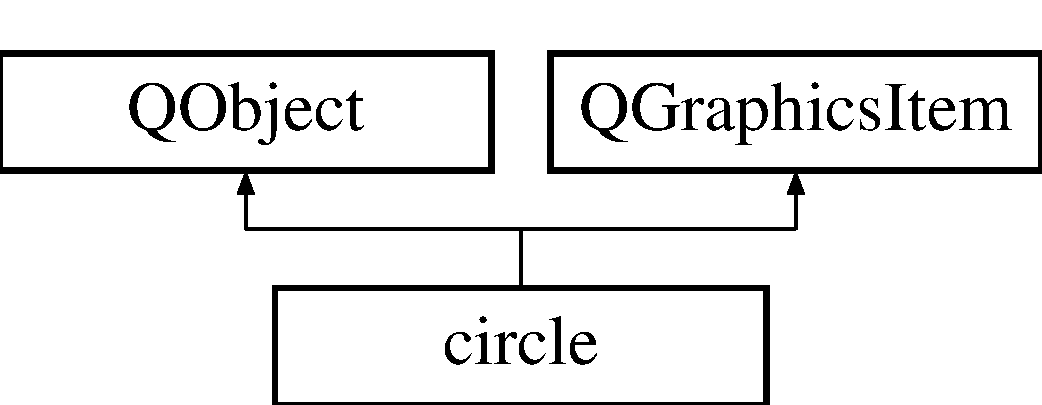
\includegraphics[height=2.000000cm]{classcircle}
\end{center}
\end{figure}
\subsection*{Public Member Functions}
\begin{DoxyCompactItemize}
\item 
\mbox{\hyperlink{classcircle_abfd721dc65145023cf14739adacc81a8}{circle}} (\mbox{\hyperlink{classgraphic_cycle}{graphic\+Cycle}} $\ast$parent, struct \mbox{\hyperlink{structcycle_data}{cycle\+Data}} data)
\begin{DoxyCompactList}\small\item\em circle\+::line Create a new circle. \end{DoxyCompactList}\item 
void \mbox{\hyperlink{classcircle_a2d9af8e86fb3605c736689a2e2566d26}{paint}} (Q\+Painter $\ast$painter, const Q\+Style\+Option\+Graphics\+Item $\ast$option, Q\+Widget $\ast$widget)
\begin{DoxyCompactList}\small\item\em \mbox{\hyperlink{classcircle_a2d9af8e86fb3605c736689a2e2566d26}{circle\+::paint}} Paint the circle on the scene. \end{DoxyCompactList}\item 
Q\+RectF \mbox{\hyperlink{classcircle_ab9d2059829ac8f0420c7e711caeb61c7}{bounding\+Rect}} () const
\begin{DoxyCompactList}\small\item\em \mbox{\hyperlink{classcircle_ab9d2059829ac8f0420c7e711caeb61c7}{circle\+::bounding\+Rect}} Define the bounding rect. \end{DoxyCompactList}\item 
Q\+Painter\+Path \mbox{\hyperlink{classcircle_a198cbcea745bd311fe91c2a23def746c}{shape}} () const
\begin{DoxyCompactList}\small\item\em \mbox{\hyperlink{classcircle_a198cbcea745bd311fe91c2a23def746c}{circle\+::shape}} Define the clipping mask of the object \end{DoxyCompactList}\end{DoxyCompactItemize}


\subsection{Constructor \& Destructor Documentation}
\mbox{\Hypertarget{classcircle_abfd721dc65145023cf14739adacc81a8}\label{classcircle_abfd721dc65145023cf14739adacc81a8}} 
\index{circle@{circle}!circle@{circle}}
\index{circle@{circle}!circle@{circle}}
\subsubsection{\texorpdfstring{circle()}{circle()}}
{\footnotesize\ttfamily circle\+::circle (\begin{DoxyParamCaption}\item[{\mbox{\hyperlink{classgraphic_cycle}{graphic\+Cycle}} $\ast$}]{parent,  }\item[{struct \mbox{\hyperlink{structcycle_data}{cycle\+Data}}}]{data }\end{DoxyParamCaption})}



circle\+::line Create a new circle. 


\begin{DoxyParams}{Parameters}
{\em struct} & \mbox{\hyperlink{structcycle_data}{cycle\+Data}} data Contains the data needed to draw the circle.\\
\hline
\end{DoxyParams}
Construct a new line on the scene and assign it to the parent \mbox{\hyperlink{classgraphic_cycle}{graphic\+Cycle}}. 

\subsection{Member Function Documentation}
\mbox{\Hypertarget{classcircle_ab9d2059829ac8f0420c7e711caeb61c7}\label{classcircle_ab9d2059829ac8f0420c7e711caeb61c7}} 
\index{circle@{circle}!bounding\+Rect@{bounding\+Rect}}
\index{bounding\+Rect@{bounding\+Rect}!circle@{circle}}
\subsubsection{\texorpdfstring{bounding\+Rect()}{boundingRect()}}
{\footnotesize\ttfamily Q\+RectF circle\+::bounding\+Rect (\begin{DoxyParamCaption}{ }\end{DoxyParamCaption}) const}



\mbox{\hyperlink{classcircle_ab9d2059829ac8f0420c7e711caeb61c7}{circle\+::bounding\+Rect}} Define the bounding rect. 

\begin{DoxyReturn}{Returns}
Q\+RectF
\end{DoxyReturn}
Define the box the object is drawn within on the scene. \mbox{\Hypertarget{classcircle_a2d9af8e86fb3605c736689a2e2566d26}\label{classcircle_a2d9af8e86fb3605c736689a2e2566d26}} 
\index{circle@{circle}!paint@{paint}}
\index{paint@{paint}!circle@{circle}}
\subsubsection{\texorpdfstring{paint()}{paint()}}
{\footnotesize\ttfamily void circle\+::paint (\begin{DoxyParamCaption}\item[{Q\+Painter $\ast$}]{painter,  }\item[{const Q\+Style\+Option\+Graphics\+Item $\ast$}]{option,  }\item[{Q\+Widget $\ast$}]{widget }\end{DoxyParamCaption})}



\mbox{\hyperlink{classcircle_a2d9af8e86fb3605c736689a2e2566d26}{circle\+::paint}} Paint the circle on the scene. 


\begin{DoxyParams}{Parameters}
{\em painter} & Q\+Painter object. \\
\hline
{\em option} & \\
\hline
{\em widget} & This function paints the point on the scene given various parameters (such as x and y). The point is drawn differently dependent on the drawing metric in use. \\
\hline
\end{DoxyParams}
\mbox{\Hypertarget{classcircle_a198cbcea745bd311fe91c2a23def746c}\label{classcircle_a198cbcea745bd311fe91c2a23def746c}} 
\index{circle@{circle}!shape@{shape}}
\index{shape@{shape}!circle@{circle}}
\subsubsection{\texorpdfstring{shape()}{shape()}}
{\footnotesize\ttfamily Q\+Painter\+Path circle\+::shape (\begin{DoxyParamCaption}{ }\end{DoxyParamCaption}) const}



\mbox{\hyperlink{classcircle_a198cbcea745bd311fe91c2a23def746c}{circle\+::shape}} Define the clipping mask of the object 

\begin{DoxyReturn}{Returns}
Q\+Painter\+Path
\end{DoxyReturn}
Defines the area in which the shape actually exists. 

The documentation for this class was generated from the following files\+:\begin{DoxyCompactItemize}
\item 
/\+Users/lukehutton/\+One\+Drive -\/ University of Leeds/\+University/\+Computer Science/\+Internship/moebinv-\/gui/include/circle.\+h\item 
/\+Users/lukehutton/\+One\+Drive -\/ University of Leeds/\+University/\+Computer Science/\+Internship/moebinv-\/gui/src/circle.\+cpp\end{DoxyCompactItemize}

\hypertarget{class_moeb_inv_1_1cycle}{}\section{Moeb\+Inv\+:\+:cycle Class Reference}
\label{class_moeb_inv_1_1cycle}\index{Moeb\+Inv\+::cycle@{Moeb\+Inv\+::cycle}}


{\ttfamily \#include $<$cycle.\+h$>$}

Inheritance diagram for Moeb\+Inv\+:\+:cycle\+:\begin{figure}[H]
\begin{center}
\leavevmode
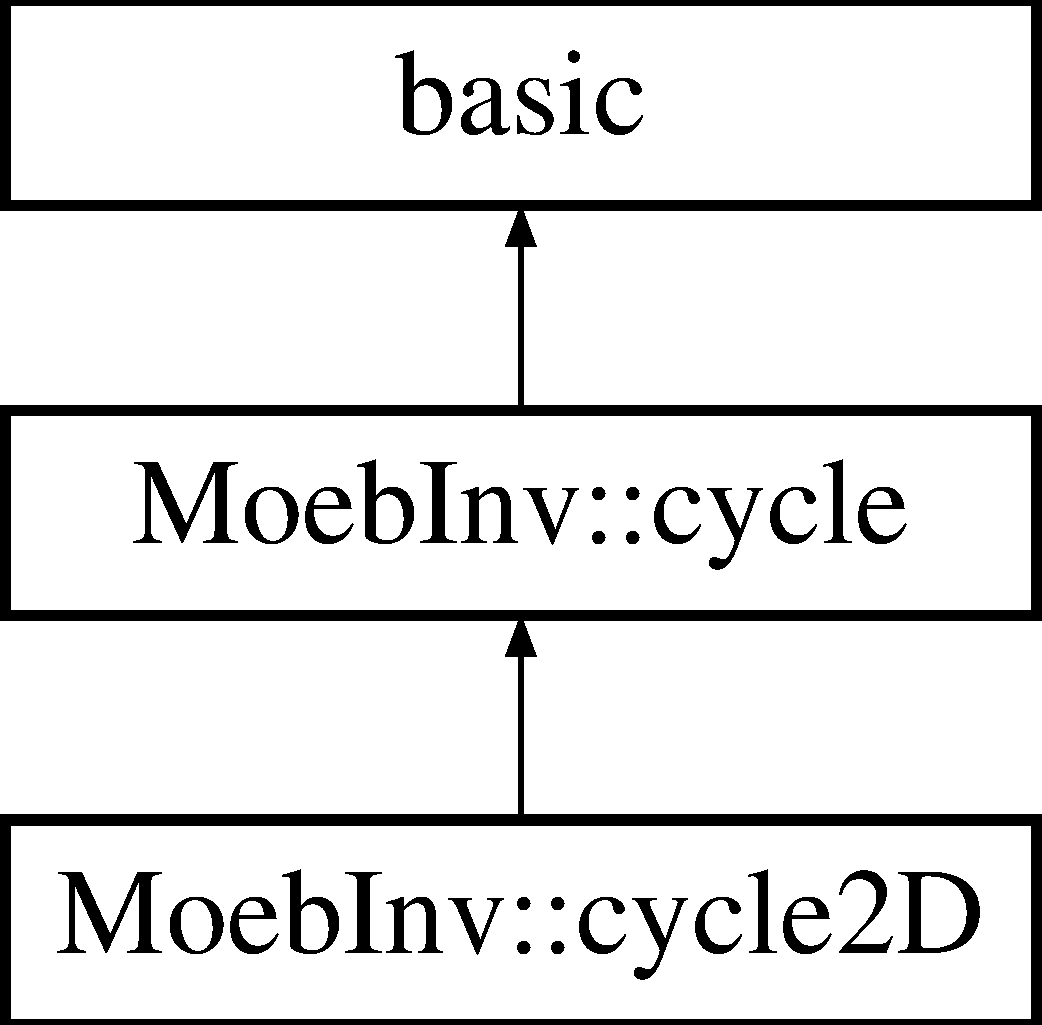
\includegraphics[height=3.000000cm]{class_moeb_inv_1_1cycle}
\end{center}
\end{figure}
\subsection*{Public Member Functions}
\begin{DoxyCompactItemize}
\item 
\mbox{\Hypertarget{class_moeb_inv_1_1cycle_a78031f0e80e19a78bb70f935625ba502}\label{class_moeb_inv_1_1cycle_a78031f0e80e19a78bb70f935625ba502}} 
{\bfseries cycle} (const ex \&k, const ex \&l, const ex \&m, const ex \&metr=-\/(new tensdelta) -\/$>$setflag(status\+\_\+flags\+::dynallocated))
\item 
\mbox{\Hypertarget{class_moeb_inv_1_1cycle_af3ca82bb271f3e385dd0c9fafdc3301d}\label{class_moeb_inv_1_1cycle_af3ca82bb271f3e385dd0c9fafdc3301d}} 
{\bfseries cycle} (const lst \&l, const ex \&metr=-\/(new tensdelta) -\/$>$setflag(status\+\_\+flags\+::dynallocated), const ex \&r\+\_\+squared=0, const ex \&e=0, const ex \&sign=(new tensdelta) -\/$>$setflag(status\+\_\+flags\+::dynallocated))
\item 
\mbox{\Hypertarget{class_moeb_inv_1_1cycle_a1835d79b682221e47f61624c1f7a7e13}\label{class_moeb_inv_1_1cycle_a1835d79b682221e47f61624c1f7a7e13}} 
{\bfseries cycle} (const \mbox{\hyperlink{class_moeb_inv_1_1cycle}{cycle}} \&C, const ex \&metr)
\item 
\mbox{\Hypertarget{class_moeb_inv_1_1cycle_a94c5100bdf9313bed7b7a1c9de4d9981}\label{class_moeb_inv_1_1cycle_a94c5100bdf9313bed7b7a1c9de4d9981}} 
{\bfseries cycle} (const matrix \&M, const ex \&metr, const ex \&e=0, const ex \&sign=0, const ex \&dim=0)
\item 
\mbox{\Hypertarget{class_moeb_inv_1_1cycle_a0f49093aa98601b3ebb17c1bd579b0d5}\label{class_moeb_inv_1_1cycle_a0f49093aa98601b3ebb17c1bd579b0d5}} 
void {\bfseries archive} (archive\+\_\+node \&n) const
\item 
\mbox{\Hypertarget{class_moeb_inv_1_1cycle_a6f81f776de51f55909b0f3804c9cf14c}\label{class_moeb_inv_1_1cycle_a6f81f776de51f55909b0f3804c9cf14c}} 
void {\bfseries read\+\_\+archive} (const archive\+\_\+node \&n, lst \&sym\+\_\+lst)
\item 
\mbox{\Hypertarget{class_moeb_inv_1_1cycle_a6ce1f343ad58eef0b8278dc5e06777b7}\label{class_moeb_inv_1_1cycle_a6ce1f343ad58eef0b8278dc5e06777b7}} 
return\+\_\+type\+\_\+t {\bfseries return\+\_\+type\+\_\+tinfo} () const
\item 
\mbox{\Hypertarget{class_moeb_inv_1_1cycle_a7218fc5ee59dd5bbbb18bf1f609cb187}\label{class_moeb_inv_1_1cycle_a7218fc5ee59dd5bbbb18bf1f609cb187}} 
ex {\bfseries real\+\_\+part} () const
\item 
\mbox{\Hypertarget{class_moeb_inv_1_1cycle_a0e001540ce76a2f5ce0c3d478707418d}\label{class_moeb_inv_1_1cycle_a0e001540ce76a2f5ce0c3d478707418d}} 
ex {\bfseries imag\+\_\+part} () const
\item 
\mbox{\Hypertarget{class_moeb_inv_1_1cycle_a547aecb94160c0ef85b30c7b719f2ad6}\label{class_moeb_inv_1_1cycle_a547aecb94160c0ef85b30c7b719f2ad6}} 
ex {\bfseries evalf} () const
\item 
\mbox{\Hypertarget{class_moeb_inv_1_1cycle_a614bac5413f4735163f62f1672a0bbef}\label{class_moeb_inv_1_1cycle_a614bac5413f4735163f62f1672a0bbef}} 
virtual ex {\bfseries get\+\_\+dim} () const
\item 
\mbox{\Hypertarget{class_moeb_inv_1_1cycle_a83acb7139250e6e1d49383bb7b6ed30e}\label{class_moeb_inv_1_1cycle_a83acb7139250e6e1d49383bb7b6ed30e}} 
virtual ex {\bfseries get\+\_\+metric} () const
\item 
\mbox{\Hypertarget{class_moeb_inv_1_1cycle_a5ca174c8add86dee778aa70aa17b96d9}\label{class_moeb_inv_1_1cycle_a5ca174c8add86dee778aa70aa17b96d9}} 
virtual ex {\bfseries get\+\_\+metric} (const ex \&i0, const ex \&i1) const
\item 
\mbox{\Hypertarget{class_moeb_inv_1_1cycle_afe1769e605e165bee92339b8a66b1351}\label{class_moeb_inv_1_1cycle_afe1769e605e165bee92339b8a66b1351}} 
virtual ex {\bfseries get\+\_\+k} () const
\item 
\mbox{\Hypertarget{class_moeb_inv_1_1cycle_a27df07a8034f526ef074ccdc4d3c388e}\label{class_moeb_inv_1_1cycle_a27df07a8034f526ef074ccdc4d3c388e}} 
ex {\bfseries get\+\_\+l} () const
\item 
\mbox{\Hypertarget{class_moeb_inv_1_1cycle_ae594b2b25786e698709db27d86b2fbac}\label{class_moeb_inv_1_1cycle_ae594b2b25786e698709db27d86b2fbac}} 
ex {\bfseries get\+\_\+l} (const ex \&i) const
\item 
\mbox{\Hypertarget{class_moeb_inv_1_1cycle_adfae0aacbda0df692a0d0d3c65943c0c}\label{class_moeb_inv_1_1cycle_adfae0aacbda0df692a0d0d3c65943c0c}} 
ex {\bfseries get\+\_\+m} () const
\item 
\mbox{\Hypertarget{class_moeb_inv_1_1cycle_a1f8a47a6a3eb3aff0fe9c845d6648d3f}\label{class_moeb_inv_1_1cycle_a1f8a47a6a3eb3aff0fe9c845d6648d3f}} 
ex {\bfseries get\+\_\+unit} () const
\item 
\mbox{\Hypertarget{class_moeb_inv_1_1cycle_ab8ebee0c26462d69e3e4da298d685184}\label{class_moeb_inv_1_1cycle_ab8ebee0c26462d69e3e4da298d685184}} 
size\+\_\+t {\bfseries nops} () const
\item 
\mbox{\Hypertarget{class_moeb_inv_1_1cycle_a0574d28f1752ff262a7b04ca05208b2e}\label{class_moeb_inv_1_1cycle_a0574d28f1752ff262a7b04ca05208b2e}} 
ex {\bfseries op} (size\+\_\+t i) const
\item 
\mbox{\Hypertarget{class_moeb_inv_1_1cycle_a07c8bf72a2f302fe559ca88774f627c1}\label{class_moeb_inv_1_1cycle_a07c8bf72a2f302fe559ca88774f627c1}} 
ex \& {\bfseries let\+\_\+op} (size\+\_\+t i)
\item 
\mbox{\Hypertarget{class_moeb_inv_1_1cycle_ad479190eaee682f3d1d993c6c11a9e7e}\label{class_moeb_inv_1_1cycle_ad479190eaee682f3d1d993c6c11a9e7e}} 
bool {\bfseries is\+\_\+equal} (const basic \&other, bool projectively=true, bool ignore\+\_\+unit=false) const
\item 
\mbox{\Hypertarget{class_moeb_inv_1_1cycle_a9d20ab2167e22304fbe729b79947270c}\label{class_moeb_inv_1_1cycle_a9d20ab2167e22304fbe729b79947270c}} 
bool {\bfseries is\+\_\+zero} () const
\item 
\mbox{\Hypertarget{class_moeb_inv_1_1cycle_aaa0d0ecddf008cafdc8b6d89d8bd1aa4}\label{class_moeb_inv_1_1cycle_aaa0d0ecddf008cafdc8b6d89d8bd1aa4}} 
\mbox{\hyperlink{class_moeb_inv_1_1cycle}{cycle}} {\bfseries subs} (const ex \&e, unsigned options=0) const
\item 
\mbox{\Hypertarget{class_moeb_inv_1_1cycle_a24f997864816a04fb22b94617540a3bc}\label{class_moeb_inv_1_1cycle_a24f997864816a04fb22b94617540a3bc}} 
\mbox{\hyperlink{class_moeb_inv_1_1cycle}{cycle}} {\bfseries normal} () const
\item 
\mbox{\Hypertarget{class_moeb_inv_1_1cycle_ad03cc19319b3cb1131a58644b1864104}\label{class_moeb_inv_1_1cycle_ad03cc19319b3cb1131a58644b1864104}} 
\mbox{\hyperlink{class_moeb_inv_1_1cycle}{cycle}} {\bfseries expand} () const
\item 
\mbox{\Hypertarget{class_moeb_inv_1_1cycle_af0209835b95128c1096b8b0d4837ed76}\label{class_moeb_inv_1_1cycle_af0209835b95128c1096b8b0d4837ed76}} 
ex {\bfseries the\+\_\+same\+\_\+as} (const basic \&other) const
\item 
\mbox{\Hypertarget{class_moeb_inv_1_1cycle_a98b8dd398f4e762adaf084a6c928d12a}\label{class_moeb_inv_1_1cycle_a98b8dd398f4e762adaf084a6c928d12a}} 
\mbox{\hyperlink{class_moeb_inv_1_1cycle}{cycle}} {\bfseries normalize\+\_\+det} (const ex \&e=0, const ex \&sign=(new tensdelta) -\/$>$setflag(status\+\_\+flags\+::dynallocated), const ex \&D=1, bool fix\+\_\+paravector=true) const
\item 
\mbox{\Hypertarget{class_moeb_inv_1_1cycle_aa90c676e4a9f1c790ed57fb3a308246c}\label{class_moeb_inv_1_1cycle_aa90c676e4a9f1c790ed57fb3a308246c}} 
\mbox{\hyperlink{class_moeb_inv_1_1cycle}{cycle}} {\bfseries normalize\+\_\+norm} (const ex \&e=0, const ex \&sign=(new tensdelta) -\/$>$setflag(status\+\_\+flags\+::dynallocated), const ex \&N=1, bool fix\+\_\+paravector=true) const
\item 
\mbox{\Hypertarget{class_moeb_inv_1_1cycle_a26c62495e60365edc320e886ec8c0aab}\label{class_moeb_inv_1_1cycle_a26c62495e60365edc320e886ec8c0aab}} 
\mbox{\hyperlink{class_moeb_inv_1_1cycle}{cycle}} {\bfseries normalize} (const ex \&k\+\_\+new=numeric(1), const ex \&e=0) const
\item 
\mbox{\Hypertarget{class_moeb_inv_1_1cycle_a468128d4fae6621ed299641998580615}\label{class_moeb_inv_1_1cycle_a468128d4fae6621ed299641998580615}} 
virtual ex {\bfseries center} (const ex \&metr=0, bool return\+\_\+matrix=false) const
\item 
\mbox{\Hypertarget{class_moeb_inv_1_1cycle_a7ab57636de7013a28889fbe91e6fbf61}\label{class_moeb_inv_1_1cycle_a7ab57636de7013a28889fbe91e6fbf61}} 
virtual ex {\bfseries val} (const ex \&y, const ex \&x=1) const
\item 
\mbox{\Hypertarget{class_moeb_inv_1_1cycle_a30908f9255f61cf3347d78112cdbadc4}\label{class_moeb_inv_1_1cycle_a30908f9255f61cf3347d78112cdbadc4}} 
ex {\bfseries passing} (const ex \&y) const
\item 
\mbox{\Hypertarget{class_moeb_inv_1_1cycle_a6bd3be5315d5a1b082befaeb5417f8c8}\label{class_moeb_inv_1_1cycle_a6bd3be5315d5a1b082befaeb5417f8c8}} 
\mbox{\hyperlink{class_moeb_inv_1_1cycle}{cycle}} {\bfseries subject\+\_\+to} (const ex \&condition, const ex \&vars=0) const
\item 
\mbox{\Hypertarget{class_moeb_inv_1_1cycle_a9ec7c783b928a2a3d8bc417524598b8a}\label{class_moeb_inv_1_1cycle_a9ec7c783b928a2a3d8bc417524598b8a}} 
virtual matrix {\bfseries to\+\_\+matrix} (const ex \&e=0, const ex \&sign=(new tensdelta) -\/$>$setflag(status\+\_\+flags\+::dynallocated), bool conjugate=false) const
\item 
\mbox{\Hypertarget{class_moeb_inv_1_1cycle_a659f15d4952b0dcd013c6f21473cf24b}\label{class_moeb_inv_1_1cycle_a659f15d4952b0dcd013c6f21473cf24b}} 
virtual ex {\bfseries det} (const ex \&e=0, const ex \&sign=(new tensdelta) -\/$>$setflag(status\+\_\+flags\+::dynallocated), const ex \&k\+\_\+norm=0, bool fix\+\_\+paravector=false) const
\item 
\mbox{\Hypertarget{class_moeb_inv_1_1cycle_ad385659a0af87a85d851a474a2d46d7c}\label{class_moeb_inv_1_1cycle_ad385659a0af87a85d851a474a2d46d7c}} 
virtual ex {\bfseries radius\+\_\+sq} (const ex \&e=0, const ex \&sign=(new tensdelta) -\/$>$setflag(status\+\_\+flags\+::dynallocated)) const
\item 
\mbox{\Hypertarget{class_moeb_inv_1_1cycle_ab4cc0f69a116bc06af1b3184078c857d}\label{class_moeb_inv_1_1cycle_ab4cc0f69a116bc06af1b3184078c857d}} 
virtual ex {\bfseries mul} (const ex \&C, const ex \&e=0, const ex \&sign=(new tensdelta) -\/$>$setflag(status\+\_\+flags\+::dynallocated), const ex \&sign1=0) const
\item 
\mbox{\Hypertarget{class_moeb_inv_1_1cycle_ad87bfcbb4f37d606d994a20358ec5d3f}\label{class_moeb_inv_1_1cycle_ad87bfcbb4f37d606d994a20358ec5d3f}} 
\mbox{\hyperlink{class_moeb_inv_1_1cycle}{cycle}} {\bfseries sl2\+\_\+similarity} (const ex \&a, const ex \&b, const ex \&c, const ex \&d, const ex \&e=0, const ex \&sign=(new tensdelta) -\/$>$setflag(status\+\_\+flags\+::dynallocated), bool not\+\_\+inverse=true, const ex \&sign\+\_\+inv=(new tensdelta) -\/$>$setflag(status\+\_\+flags\+::dynallocated)) const
\item 
\mbox{\Hypertarget{class_moeb_inv_1_1cycle_a8a87c052f2d9128b3137186da05ff22d}\label{class_moeb_inv_1_1cycle_a8a87c052f2d9128b3137186da05ff22d}} 
\mbox{\hyperlink{class_moeb_inv_1_1cycle}{cycle}} {\bfseries sl2\+\_\+similarity} (const ex \&M, const ex \&e=0, const ex \&sign=(new tensdelta) -\/$>$setflag(status\+\_\+flags\+::dynallocated), bool not\+\_\+inverse=true, const ex \&sign\+\_\+inv=(new tensdelta) -\/$>$setflag(status\+\_\+flags\+::dynallocated)) const
\item 
\mbox{\Hypertarget{class_moeb_inv_1_1cycle_a5c31fa1602c633af97f7703436d59392}\label{class_moeb_inv_1_1cycle_a5c31fa1602c633af97f7703436d59392}} 
virtual \mbox{\hyperlink{class_moeb_inv_1_1cycle}{cycle}} {\bfseries matrix\+\_\+similarity} (const ex \&M, const ex \&e=0, const ex \&sign=(new tensdelta) -\/$>$setflag(status\+\_\+flags\+::dynallocated), bool not\+\_\+inverse=true, const ex \&sign\+\_\+inv=(new tensdelta) -\/$>$setflag(status\+\_\+flags\+::dynallocated)) const
\item 
\mbox{\Hypertarget{class_moeb_inv_1_1cycle_a571d091fd4e98904d7ae878f244dd549}\label{class_moeb_inv_1_1cycle_a571d091fd4e98904d7ae878f244dd549}} 
virtual \mbox{\hyperlink{class_moeb_inv_1_1cycle}{cycle}} {\bfseries matrix\+\_\+similarity} (const ex \&a, const ex \&b, const ex \&c, const ex \&d, const ex \&e=0, const ex \&sign=(new tensdelta) -\/$>$setflag(status\+\_\+flags\+::dynallocated), bool not\+\_\+inverse=true, const ex \&sign\+\_\+inv=(new tensdelta) -\/$>$setflag(status\+\_\+flags\+::dynallocated)) const
\item 
\mbox{\Hypertarget{class_moeb_inv_1_1cycle_a0064156ee80dc1f1f6a1d3360d48f9a2}\label{class_moeb_inv_1_1cycle_a0064156ee80dc1f1f6a1d3360d48f9a2}} 
virtual \mbox{\hyperlink{class_moeb_inv_1_1cycle}{cycle}} {\bfseries cycle\+\_\+similarity} (const \mbox{\hyperlink{class_moeb_inv_1_1cycle}{cycle}} \&C, const ex \&e=0, const ex \&sign=(new tensdelta) -\/$>$setflag(status\+\_\+flags\+::dynallocated), const ex \&sign1=0, const ex \&sign\+\_\+inv=(new tensdelta) -\/$>$setflag(status\+\_\+flags\+::dynallocated)) const
\item 
\mbox{\Hypertarget{class_moeb_inv_1_1cycle_aec17175f191a94d6654a69073ca6a864}\label{class_moeb_inv_1_1cycle_aec17175f191a94d6654a69073ca6a864}} 
virtual ex {\bfseries moebius\+\_\+map} (const ex \&P, const ex \&e=0, const ex \&sign=(new tensdelta) -\/$>$setflag(status\+\_\+flags\+::dynallocated)) const
\item 
\mbox{\Hypertarget{class_moeb_inv_1_1cycle_adbaf9c9cbde860cbfefcb89fa0f873d5}\label{class_moeb_inv_1_1cycle_adbaf9c9cbde860cbfefcb89fa0f873d5}} 
virtual ex {\bfseries cycle\+\_\+product} (const \mbox{\hyperlink{class_moeb_inv_1_1cycle}{cycle}} \&C, const ex \&e=0, const ex \&sign=(new tensdelta) -\/$>$setflag(status\+\_\+flags\+::dynallocated)) const
\item 
\mbox{\Hypertarget{class_moeb_inv_1_1cycle_ab76631c75b0a092cc3bd5959f5a45a99}\label{class_moeb_inv_1_1cycle_ab76631c75b0a092cc3bd5959f5a45a99}} 
virtual ex {\bfseries is\+\_\+orthogonal} (const \mbox{\hyperlink{class_moeb_inv_1_1cycle}{cycle}} \&C, const ex \&e=0, const ex \&sign=(new tensdelta) -\/$>$setflag(status\+\_\+flags\+::dynallocated)) const
\item 
\mbox{\Hypertarget{class_moeb_inv_1_1cycle_a2c94a9eda34309d9ff2baa11e98dcffb}\label{class_moeb_inv_1_1cycle_a2c94a9eda34309d9ff2baa11e98dcffb}} 
ex {\bfseries is\+\_\+f\+\_\+orthogonal} (const \mbox{\hyperlink{class_moeb_inv_1_1cycle}{cycle}} \&C, const ex \&e=0, const ex \&sign=(new tensdelta) -\/$>$setflag(status\+\_\+flags\+::dynallocated), const ex \&sign1=0, const ex \&sign\+\_\+inv=(new tensdelta) -\/$>$setflag(status\+\_\+flags\+::dynallocated)) const
\item 
\mbox{\Hypertarget{class_moeb_inv_1_1cycle_ae932ea0e679982cb9a8913002705dc4d}\label{class_moeb_inv_1_1cycle_ae932ea0e679982cb9a8913002705dc4d}} 
ex {\bfseries is\+\_\+linear} () const
\item 
\mbox{\Hypertarget{class_moeb_inv_1_1cycle_a428d54de886680e1aea3b93bb6da259a}\label{class_moeb_inv_1_1cycle_a428d54de886680e1aea3b93bb6da259a}} 
ex {\bfseries is\+\_\+normalized} () const
\item 
\mbox{\Hypertarget{class_moeb_inv_1_1cycle_a3dea21b462eb2ccc321716c2c23f6409}\label{class_moeb_inv_1_1cycle_a3dea21b462eb2ccc321716c2c23f6409}} 
virtual \mbox{\hyperlink{class_moeb_inv_1_1cycle}{cycle}} {\bfseries add} (const \mbox{\hyperlink{class_moeb_inv_1_1cycle}{cycle}} \&rh) const
\item 
\mbox{\Hypertarget{class_moeb_inv_1_1cycle_a3a4f7d977cfb2ed4025ba9013e229e27}\label{class_moeb_inv_1_1cycle_a3a4f7d977cfb2ed4025ba9013e229e27}} 
virtual \mbox{\hyperlink{class_moeb_inv_1_1cycle}{cycle}} {\bfseries sub} (const \mbox{\hyperlink{class_moeb_inv_1_1cycle}{cycle}} \&rh) const
\item 
\mbox{\Hypertarget{class_moeb_inv_1_1cycle_a8d187b8a78f64c038bc4722903501c74}\label{class_moeb_inv_1_1cycle_a8d187b8a78f64c038bc4722903501c74}} 
virtual \mbox{\hyperlink{class_moeb_inv_1_1cycle}{cycle}} {\bfseries exmul} (const ex \&rh) const
\item 
\mbox{\Hypertarget{class_moeb_inv_1_1cycle_ac10ea6fcc2b7aaf185379a6dd77e97bf}\label{class_moeb_inv_1_1cycle_ac10ea6fcc2b7aaf185379a6dd77e97bf}} 
virtual \mbox{\hyperlink{class_moeb_inv_1_1cycle}{cycle}} {\bfseries div} (const ex \&rh) const
\end{DoxyCompactItemize}
\subsection*{Protected Member Functions}
\begin{DoxyCompactItemize}
\item 
\mbox{\Hypertarget{class_moeb_inv_1_1cycle_a480825f714ac1daf43930434eaed8cd0}\label{class_moeb_inv_1_1cycle_a480825f714ac1daf43930434eaed8cd0}} 
void {\bfseries do\+\_\+print} (const print\+\_\+dflt \&c, unsigned level) const
\item 
\mbox{\Hypertarget{class_moeb_inv_1_1cycle_accf05994662b590d40ada1615ce5cc2c}\label{class_moeb_inv_1_1cycle_accf05994662b590d40ada1615ce5cc2c}} 
void {\bfseries do\+\_\+print\+\_\+dflt} (const print\+\_\+dflt \&c, unsigned level) const
\item 
\mbox{\Hypertarget{class_moeb_inv_1_1cycle_af155c4801d08afadeba7365df94ca934}\label{class_moeb_inv_1_1cycle_af155c4801d08afadeba7365df94ca934}} 
void {\bfseries do\+\_\+print\+\_\+latex} (const print\+\_\+latex \&c, unsigned level) const
\end{DoxyCompactItemize}
\subsection*{Protected Attributes}
\begin{DoxyCompactItemize}
\item 
\mbox{\Hypertarget{class_moeb_inv_1_1cycle_a24cfb770bb714d257c73f277b6907d87}\label{class_moeb_inv_1_1cycle_a24cfb770bb714d257c73f277b6907d87}} 
ex {\bfseries unit}
\item 
\mbox{\Hypertarget{class_moeb_inv_1_1cycle_a011e43461950d16ae980cfb73b446827}\label{class_moeb_inv_1_1cycle_a011e43461950d16ae980cfb73b446827}} 
ex {\bfseries k}
\item 
\mbox{\Hypertarget{class_moeb_inv_1_1cycle_afb8241122390156518d2dee04e3df2e6}\label{class_moeb_inv_1_1cycle_afb8241122390156518d2dee04e3df2e6}} 
ex {\bfseries l}
\item 
\mbox{\Hypertarget{class_moeb_inv_1_1cycle_a2b064bd63cc048aef8433252b1c35d6a}\label{class_moeb_inv_1_1cycle_a2b064bd63cc048aef8433252b1c35d6a}} 
ex {\bfseries m}
\end{DoxyCompactItemize}


\subsection{Detailed Description}
The class holding cycles kx$^\wedge$2-\/2$<$l,x$>$+m=0 

The documentation for this class was generated from the following files\+:\begin{DoxyCompactItemize}
\item 
/\+Users/lukehutton/\+One\+Drive -\/ University of Leeds/\+University/\+Computer Science/\+Internship/moebinv-\/gui/lib/moebinv-\/3.\+2/include/cycle.\+h\item 
/\+Users/lukehutton/\+One\+Drive -\/ University of Leeds/\+University/\+Computer Science/\+Internship/moebinv-\/gui/lib/moebinv-\/3.\+2/src/cycle.\+cpp\end{DoxyCompactItemize}

\hypertarget{class_moeb_inv_1_1cycle2_d}{}\section{Moeb\+Inv\+:\+:cycle2D Class Reference}
\label{class_moeb_inv_1_1cycle2_d}\index{Moeb\+Inv\+::cycle2D@{Moeb\+Inv\+::cycle2D}}
Inheritance diagram for Moeb\+Inv\+:\+:cycle2D\+:\begin{figure}[H]
\begin{center}
\leavevmode
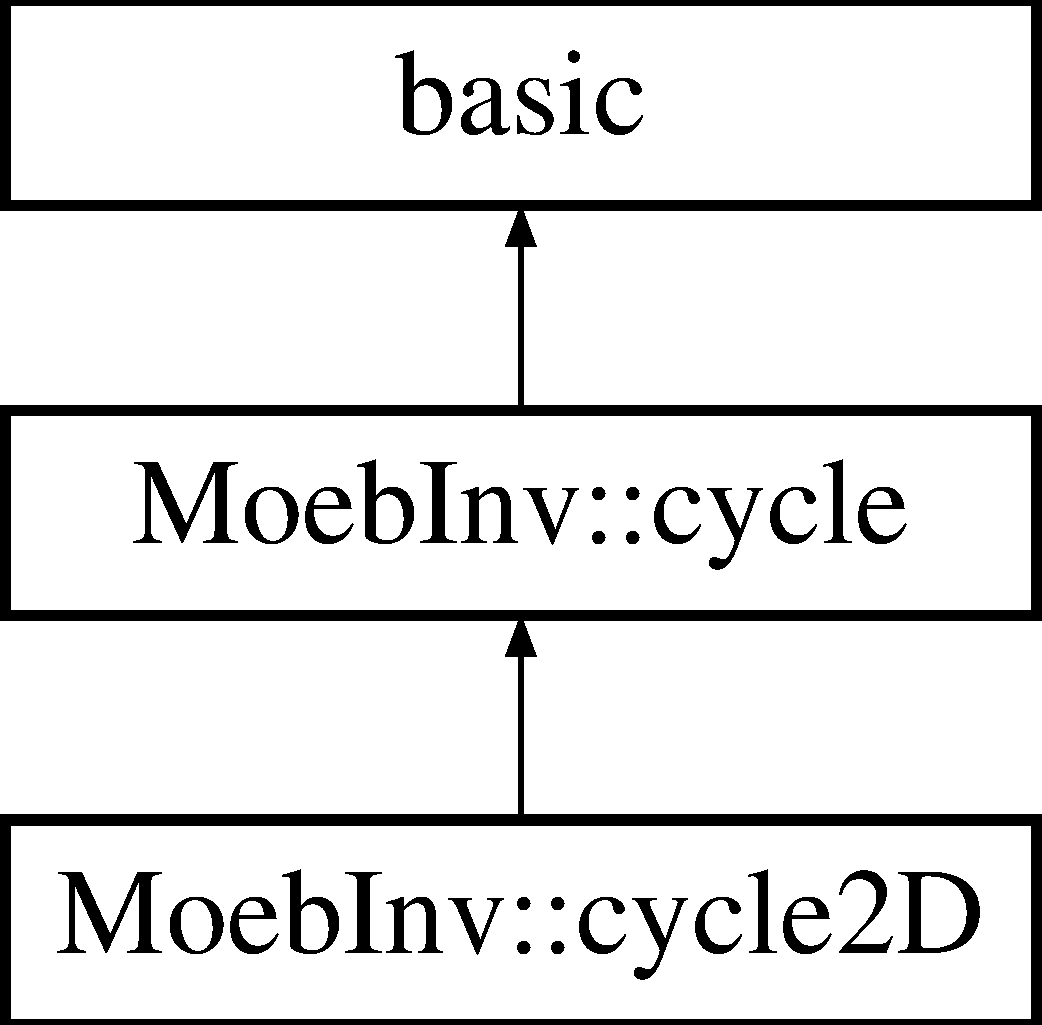
\includegraphics[height=3.000000cm]{class_moeb_inv_1_1cycle2_d}
\end{center}
\end{figure}
\subsection*{Public Member Functions}
\begin{DoxyCompactItemize}
\item 
\mbox{\Hypertarget{class_moeb_inv_1_1cycle2_d_a6d68a6e30401e78728f0b89ab1630921}\label{class_moeb_inv_1_1cycle2_d_a6d68a6e30401e78728f0b89ab1630921}} 
{\bfseries cycle2D} (const ex \&k1, const ex \&l1, const ex \&m1, const ex \&metr=-\/unit\+\_\+matrix(2))
\item 
\mbox{\Hypertarget{class_moeb_inv_1_1cycle2_d_af9452b92d2c0e76f6e7d8f45b1ecd44d}\label{class_moeb_inv_1_1cycle2_d_af9452b92d2c0e76f6e7d8f45b1ecd44d}} 
{\bfseries cycle2D} (const lst \&l, const ex \&metr=-\/unit\+\_\+matrix(2), const ex \&r\+\_\+squared=0, const ex \&e=0, const ex \&sign=unit\+\_\+matrix(2))
\item 
\mbox{\Hypertarget{class_moeb_inv_1_1cycle2_d_ad367447c0c69cb23a031ff6252867399}\label{class_moeb_inv_1_1cycle2_d_ad367447c0c69cb23a031ff6252867399}} 
{\bfseries cycle2D} (const matrix \&M, const ex \&metr, const ex \&e=0, const ex \&sign=0)
\item 
\mbox{\Hypertarget{class_moeb_inv_1_1cycle2_d_a18cf99dad3f906e4a759f5424ae12430}\label{class_moeb_inv_1_1cycle2_d_a18cf99dad3f906e4a759f5424ae12430}} 
{\bfseries cycle2D} (const \mbox{\hyperlink{class_moeb_inv_1_1cycle}{cycle}} \&C, const ex \&metr=0)
\item 
\mbox{\Hypertarget{class_moeb_inv_1_1cycle2_d_a657820f5e271de26192593a763624ce2}\label{class_moeb_inv_1_1cycle2_d_a657820f5e271de26192593a763624ce2}} 
virtual ex {\bfseries hdet} (const ex \&e=0, const ex \&sign=(new tensdelta) -\/$>$setflag(status\+\_\+flags\+::dynallocated), const ex \&k\+\_\+norm=0) const
\item 
\mbox{\Hypertarget{class_moeb_inv_1_1cycle2_d_ab96a9e3b049ac9773c2331659e001b57}\label{class_moeb_inv_1_1cycle2_d_ab96a9e3b049ac9773c2331659e001b57}} 
ex {\bfseries focus} (const ex \&e=diag\+\_\+matrix(lst\{-\/1, 1\}), bool return\+\_\+matrix=false) const
\item 
\mbox{\Hypertarget{class_moeb_inv_1_1cycle2_d_a40015b98c8423a741470d4e0ea39f8ed}\label{class_moeb_inv_1_1cycle2_d_a40015b98c8423a741470d4e0ea39f8ed}} 
ex {\bfseries focal\+\_\+length} () const
\item 
\mbox{\Hypertarget{class_moeb_inv_1_1cycle2_d_a6ad3dc95ef86904f04c652e88c6a2712}\label{class_moeb_inv_1_1cycle2_d_a6ad3dc95ef86904f04c652e88c6a2712}} 
lst {\bfseries roots} (const ex \&y=0, bool first=true) const
\item 
\mbox{\Hypertarget{class_moeb_inv_1_1cycle2_d_a006c6e8a216cee4e6fa1df8fff7f6f8e}\label{class_moeb_inv_1_1cycle2_d_a006c6e8a216cee4e6fa1df8fff7f6f8e}} 
lst {\bfseries line\+\_\+intersect} (const ex \&a, const ex \&b) const
\item 
\mbox{\Hypertarget{class_moeb_inv_1_1cycle2_d_a303f13dc4acb34bd4872d6152d46d8ea}\label{class_moeb_inv_1_1cycle2_d_a303f13dc4acb34bd4872d6152d46d8ea}} 
void {\bfseries metapost\+\_\+draw} (ostream \&ost, const ex \&xmin=-\/5, const ex \&xmax=5, const ex \&ymin=-\/5, const ex \&ymax=5, const lst \&color=lst\{\}, const string more\+\_\+options=\char`\"{}\char`\"{}, bool with\+\_\+header=true, int points\+\_\+per\+\_\+arc=0, bool asymptote=false, const string picture=\char`\"{}\char`\"{}, bool only\+\_\+path=false, bool is\+\_\+continuation=false, const string imaginary\+\_\+options=\char`\"{}withcolor .\+9$\ast$green withpen pencircle scaled 4pt\char`\"{}) const
\item 
\mbox{\Hypertarget{class_moeb_inv_1_1cycle2_d_af6d5250d65c5b89c2ad26a3870260d52}\label{class_moeb_inv_1_1cycle2_d_af6d5250d65c5b89c2ad26a3870260d52}} 
\mbox{\hyperlink{class_moeb_inv_1_1cycle2_d}{cycle2D}} {\bfseries sl2\+\_\+similarity} (const ex \&M1, const ex \&M2, const ex \&e, const ex \&sign, bool not\+\_\+inverse=true, const ex \&sign\+\_\+inv=(new tensdelta) -\/$>$setflag(status\+\_\+flags\+::dynallocated)) const
\item 
\mbox{\Hypertarget{class_moeb_inv_1_1cycle2_d_ad53312cabcf0a9c4356cc766ddb301ab}\label{class_moeb_inv_1_1cycle2_d_ad53312cabcf0a9c4356cc766ddb301ab}} 
\mbox{\hyperlink{class_moeb_inv_1_1cycle2_d}{cycle2D}} {\bfseries sl2\+\_\+similarity} (const ex \&a1, const ex \&b1, const ex \&c1, const ex \&d1, const ex \&a2, const ex \&b2, const ex \&c2, const ex \&d2, const ex \&e=0, const ex \&sign=(new tensdelta) -\/$>$setflag(status\+\_\+flags\+::dynallocated), bool not\+\_\+inverse=true, const ex \&sign\+\_\+inv=(new tensdelta) -\/$>$setflag(status\+\_\+flags\+::dynallocated)) const
\item 
\mbox{\Hypertarget{class_moeb_inv_1_1cycle2_d_a2af30738cf483468f03ac800c102c62a}\label{class_moeb_inv_1_1cycle2_d_a2af30738cf483468f03ac800c102c62a}} 
void {\bfseries asy\+\_\+draw} (ostream \&ost, const string picture, const ex \&xmin=-\/5, const ex \&xmax=5, const ex \&ymin=-\/5, const ex \&ymax=5, const lst \&color=lst\{\}, const string more\+\_\+options=\char`\"{}\char`\"{}, bool with\+\_\+header=true, int points\+\_\+per\+\_\+arc=0, const string imaginary\+\_\+options=\char`\"{}rgb(0,.\+9,0)+4pt\char`\"{}) const
\item 
\mbox{\Hypertarget{class_moeb_inv_1_1cycle2_d_a46c94eb343ee725668fc5eb53a04bd3d}\label{class_moeb_inv_1_1cycle2_d_a46c94eb343ee725668fc5eb53a04bd3d}} 
void {\bfseries asy\+\_\+draw} (ostream \&ost=std\+::cout, const ex \&xmin=-\/5, const ex \&xmax=5, const ex \&ymin=-\/5, const ex \&ymax=5, const lst \&color=lst\{\}, const string more\+\_\+options=\char`\"{}\char`\"{}, bool with\+\_\+header=true, int points\+\_\+per\+\_\+arc=0, const string imaginary\+\_\+options=\char`\"{}rgb(0,.\+9,0)+4pt\char`\"{}) const
\item 
\mbox{\Hypertarget{class_moeb_inv_1_1cycle2_d_a278dda55874cd3cf848f302ef6dafe0e}\label{class_moeb_inv_1_1cycle2_d_a278dda55874cd3cf848f302ef6dafe0e}} 
void {\bfseries asy\+\_\+path} (ostream \&ost=std\+::cout, const ex \&xmin=-\/5, const ex \&xmax=5, const ex \&ymin=-\/5, const ex \&ymax=5, int points\+\_\+per\+\_\+arc=0, bool is\+\_\+continuation=false) const
\item 
\mbox{\Hypertarget{class_moeb_inv_1_1cycle2_d_ad0170765bc192ecab6c4b0036952afb1}\label{class_moeb_inv_1_1cycle2_d_ad0170765bc192ecab6c4b0036952afb1}} 
\mbox{\hyperlink{class_moeb_inv_1_1cycle2_d}{cycle2D}} {\bfseries subs} (const ex \&e, unsigned options=0) const
\item 
\mbox{\Hypertarget{class_moeb_inv_1_1cycle2_d_a593692e6c3e39757b5df6d00984b53ba}\label{class_moeb_inv_1_1cycle2_d_a593692e6c3e39757b5df6d00984b53ba}} 
\mbox{\hyperlink{class_moeb_inv_1_1cycle2_d}{cycle2D}} {\bfseries normalize} (const ex \&k\+\_\+new=numeric(1), const ex \&e=0) const
\item 
\mbox{\Hypertarget{class_moeb_inv_1_1cycle2_d_a73a45bda26754cd4dd62146d2a64cd3d}\label{class_moeb_inv_1_1cycle2_d_a73a45bda26754cd4dd62146d2a64cd3d}} 
\mbox{\hyperlink{class_moeb_inv_1_1cycle2_d}{cycle2D}} {\bfseries normalize\+\_\+det} (const ex \&e=0, const ex \&sign=(new tensdelta) -\/$>$setflag(status\+\_\+flags\+::dynallocated), const ex \&D=1, bool fix\+\_\+paravector=true) const
\item 
\mbox{\Hypertarget{class_moeb_inv_1_1cycle2_d_a72dfb32e4fa2ef6a02a650575a5ae65b}\label{class_moeb_inv_1_1cycle2_d_a72dfb32e4fa2ef6a02a650575a5ae65b}} 
\mbox{\hyperlink{class_moeb_inv_1_1cycle2_d}{cycle2D}} {\bfseries normalize\+\_\+norm} (const ex \&e=0, const ex \&sign=(new tensdelta) -\/$>$setflag(status\+\_\+flags\+::dynallocated), const ex \&N=1, bool fix\+\_\+paravector=true) const
\item 
\mbox{\Hypertarget{class_moeb_inv_1_1cycle2_d_a32780a0a370c0b6151648cb2efb3a24b}\label{class_moeb_inv_1_1cycle2_d_a32780a0a370c0b6151648cb2efb3a24b}} 
\mbox{\hyperlink{class_moeb_inv_1_1cycle2_d}{cycle2D}} {\bfseries sl2\+\_\+similarity} (const ex \&a, const ex \&b, const ex \&c, const ex \&d, const ex \&e=0, const ex \&sign=(new tensdelta) -\/$>$setflag(status\+\_\+flags\+::dynallocated), bool not\+\_\+inverse=true, const ex \&sign\+\_\+inv=(new tensdelta) -\/$>$setflag(status\+\_\+flags\+::dynallocated)) const
\item 
\mbox{\Hypertarget{class_moeb_inv_1_1cycle2_d_a0bf048ab4e38bf5e97768e8b487133a7}\label{class_moeb_inv_1_1cycle2_d_a0bf048ab4e38bf5e97768e8b487133a7}} 
\mbox{\hyperlink{class_moeb_inv_1_1cycle2_d}{cycle2D}} {\bfseries sl2\+\_\+similarity} (const ex \&M) const
\item 
\mbox{\Hypertarget{class_moeb_inv_1_1cycle2_d_aa8f61f0344737af159983fc2f826296f}\label{class_moeb_inv_1_1cycle2_d_aa8f61f0344737af159983fc2f826296f}} 
\mbox{\hyperlink{class_moeb_inv_1_1cycle2_d}{cycle2D}} {\bfseries sl2\+\_\+similarity} (const ex \&M, const ex \&e) const
\item 
\mbox{\Hypertarget{class_moeb_inv_1_1cycle2_d_a0f2e64f2a6242ad4ad70165311c00c52}\label{class_moeb_inv_1_1cycle2_d_a0f2e64f2a6242ad4ad70165311c00c52}} 
\mbox{\hyperlink{class_moeb_inv_1_1cycle2_d}{cycle2D}} {\bfseries sl2\+\_\+similarity} (const ex \&M, const ex \&e, const ex \&sign) const
\item 
\mbox{\Hypertarget{class_moeb_inv_1_1cycle2_d_aac7c5d4c1f9e566cfb310dda8c7bba10}\label{class_moeb_inv_1_1cycle2_d_aac7c5d4c1f9e566cfb310dda8c7bba10}} 
\mbox{\hyperlink{class_moeb_inv_1_1cycle2_d}{cycle2D}} {\bfseries sl2\+\_\+similarity} (const ex \&M, const ex \&e, const ex \&sign, bool not\+\_\+inverse, const ex \&sign\+\_\+inv=(new tensdelta) -\/$>$setflag(status\+\_\+flags\+::dynallocated)) const
\item 
\mbox{\Hypertarget{class_moeb_inv_1_1cycle2_d_abd85b44a39704e5459eab9620d5d6ec5}\label{class_moeb_inv_1_1cycle2_d_abd85b44a39704e5459eab9620d5d6ec5}} 
\mbox{\hyperlink{class_moeb_inv_1_1cycle2_d}{cycle2D}} {\bfseries normal} () const
\item 
\mbox{\Hypertarget{class_moeb_inv_1_1cycle2_d_a6f8a9b46040a85dd89ef41af946311c4}\label{class_moeb_inv_1_1cycle2_d_a6f8a9b46040a85dd89ef41af946311c4}} 
\mbox{\hyperlink{class_moeb_inv_1_1cycle2_d}{cycle2D}} {\bfseries expand} () const
\item 
\mbox{\Hypertarget{class_moeb_inv_1_1cycle2_d_aa14f443442b57392d563119e52efc7c2}\label{class_moeb_inv_1_1cycle2_d_aa14f443442b57392d563119e52efc7c2}} 
ex {\bfseries evalf} () const
\item 
\mbox{\Hypertarget{class_moeb_inv_1_1cycle2_d_ac4210321a02f39f5bf1c04aee1d9142b}\label{class_moeb_inv_1_1cycle2_d_ac4210321a02f39f5bf1c04aee1d9142b}} 
\mbox{\hyperlink{class_moeb_inv_1_1cycle2_d}{cycle2D}} {\bfseries subject\+\_\+to} (const ex \&condition, const ex \&vars=0) const
\item 
\mbox{\Hypertarget{class_moeb_inv_1_1cycle2_d_a530eb35e47b47a497bbb301dd041c3a2}\label{class_moeb_inv_1_1cycle2_d_a530eb35e47b47a497bbb301dd041c3a2}} 
void {\bfseries archive} (archive\+\_\+node \&n) const
\item 
\mbox{\Hypertarget{class_moeb_inv_1_1cycle2_d_a7d1da2385f403d7e7882ac244a37ae28}\label{class_moeb_inv_1_1cycle2_d_a7d1da2385f403d7e7882ac244a37ae28}} 
void {\bfseries read\+\_\+archive} (const archive\+\_\+node \&n, lst \&sym\+\_\+lst)
\item 
\mbox{\Hypertarget{class_moeb_inv_1_1cycle2_d_a35387bf646d1059bae865598759c6ce4}\label{class_moeb_inv_1_1cycle2_d_a35387bf646d1059bae865598759c6ce4}} 
ex {\bfseries real\+\_\+part} () const
\item 
\mbox{\Hypertarget{class_moeb_inv_1_1cycle2_d_a78c4ec1b31bdb419fa8a23c225bba587}\label{class_moeb_inv_1_1cycle2_d_a78c4ec1b31bdb419fa8a23c225bba587}} 
ex {\bfseries imag\+\_\+part} () const
\end{DoxyCompactItemize}
\subsection*{Additional Inherited Members}


The documentation for this class was generated from the following files\+:\begin{DoxyCompactItemize}
\item 
/\+Users/lukehutton/\+One\+Drive -\/ University of Leeds/\+University/\+Computer Science/\+Internship/moebinv-\/gui/lib/moebinv-\/3.\+2/include/cycle.\+h\item 
/\+Users/lukehutton/\+One\+Drive -\/ University of Leeds/\+University/\+Computer Science/\+Internship/moebinv-\/gui/lib/moebinv-\/3.\+2/src/cycle.\+cpp\end{DoxyCompactItemize}

\hypertarget{class_moeb_inv_1_1cycle__data}{}\section{Moeb\+Inv\+:\+:cycle\+\_\+data Class Reference}
\label{class_moeb_inv_1_1cycle__data}\index{Moeb\+Inv\+::cycle\+\_\+data@{Moeb\+Inv\+::cycle\+\_\+data}}
Inheritance diagram for Moeb\+Inv\+:\+:cycle\+\_\+data\+:\begin{figure}[H]
\begin{center}
\leavevmode
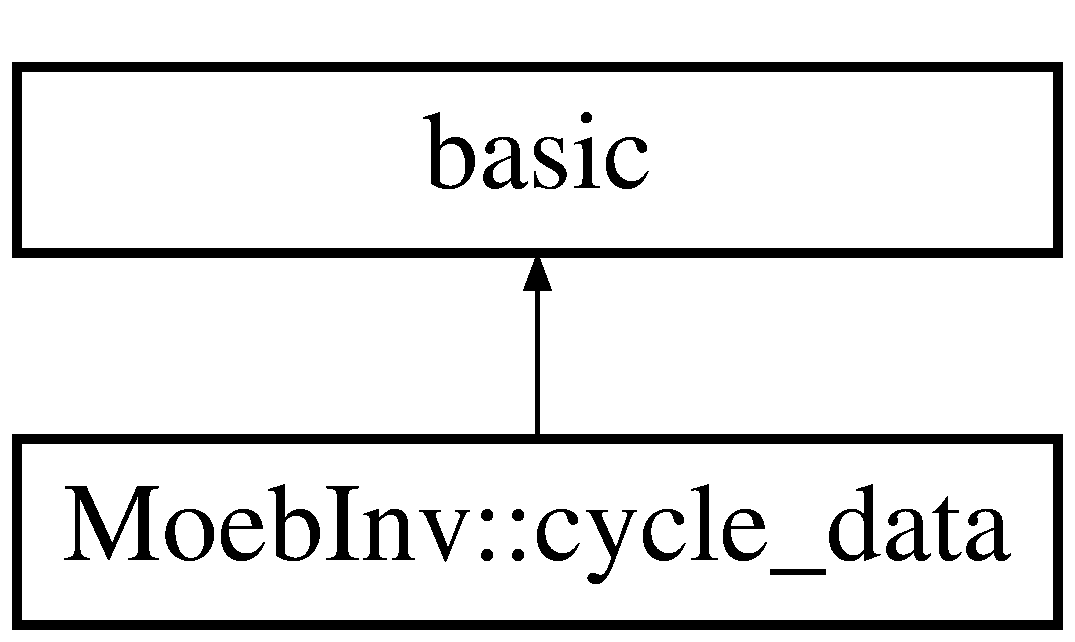
\includegraphics[height=2.000000cm]{class_moeb_inv_1_1cycle__data}
\end{center}
\end{figure}
\subsection*{Public Member Functions}
\begin{DoxyCompactItemize}
\item 
\mbox{\Hypertarget{class_moeb_inv_1_1cycle__data_a663f4881bd39482833c3a286f042180b}\label{class_moeb_inv_1_1cycle__data_a663f4881bd39482833c3a286f042180b}} 
{\bfseries cycle\+\_\+data} (const ex \&C)
\item 
\mbox{\Hypertarget{class_moeb_inv_1_1cycle__data_a3cf7bb544796c23210fa9f1295cd5056}\label{class_moeb_inv_1_1cycle__data_a3cf7bb544796c23210fa9f1295cd5056}} 
{\bfseries cycle\+\_\+data} (const ex \&k1, const ex l1, const ex \&m1, bool normalize=false)
\item 
\mbox{\Hypertarget{class_moeb_inv_1_1cycle__data_a5a5247e7df39d6562828a0ea15ecaa24}\label{class_moeb_inv_1_1cycle__data_a5a5247e7df39d6562828a0ea15ecaa24}} 
ex {\bfseries make\+\_\+cycle} (const ex \&metr) const
\item 
\mbox{\Hypertarget{class_moeb_inv_1_1cycle__data_aa051c6565f1d04ad8567878c43aa206a}\label{class_moeb_inv_1_1cycle__data_aa051c6565f1d04ad8567878c43aa206a}} 
size\+\_\+t {\bfseries nops} () const
\item 
\mbox{\Hypertarget{class_moeb_inv_1_1cycle__data_a83456262104d3cdc43d1b7a41bd3bf67}\label{class_moeb_inv_1_1cycle__data_a83456262104d3cdc43d1b7a41bd3bf67}} 
ex {\bfseries op} (size\+\_\+t i) const
\item 
\mbox{\Hypertarget{class_moeb_inv_1_1cycle__data_a7b3324e58cfd67f6d5a0dfca61b27958}\label{class_moeb_inv_1_1cycle__data_a7b3324e58cfd67f6d5a0dfca61b27958}} 
ex \& {\bfseries let\+\_\+op} (size\+\_\+t i)
\item 
\mbox{\Hypertarget{class_moeb_inv_1_1cycle__data_a4972f8fb7fb211878540c3159ad11905}\label{class_moeb_inv_1_1cycle__data_a4972f8fb7fb211878540c3159ad11905}} 
ex {\bfseries get\+\_\+k} () const
\item 
\mbox{\Hypertarget{class_moeb_inv_1_1cycle__data_a67fecf1fb0409c22460c8611f41c335a}\label{class_moeb_inv_1_1cycle__data_a67fecf1fb0409c22460c8611f41c335a}} 
ex {\bfseries get\+\_\+l} () const
\item 
\mbox{\Hypertarget{class_moeb_inv_1_1cycle__data_a936576cdde90230b7ae62c044c8ff0cd}\label{class_moeb_inv_1_1cycle__data_a936576cdde90230b7ae62c044c8ff0cd}} 
ex {\bfseries get\+\_\+l} (size\+\_\+t i) const
\item 
\mbox{\Hypertarget{class_moeb_inv_1_1cycle__data_a40d7c531c8db470cea3561d366ce0f6d}\label{class_moeb_inv_1_1cycle__data_a40d7c531c8db470cea3561d366ce0f6d}} 
ex {\bfseries get\+\_\+m} () const
\item 
\mbox{\Hypertarget{class_moeb_inv_1_1cycle__data_ae8ac42662e223cd0bcc1c183ad3dc63f}\label{class_moeb_inv_1_1cycle__data_ae8ac42662e223cd0bcc1c183ad3dc63f}} 
long unsigned int {\bfseries get\+\_\+dim} () const
\item 
\mbox{\Hypertarget{class_moeb_inv_1_1cycle__data_a9717902ddc67445f59435bb337c28911}\label{class_moeb_inv_1_1cycle__data_a9717902ddc67445f59435bb337c28911}} 
void {\bfseries do\+\_\+print} (const print\+\_\+dflt \&con, unsigned level) const
\item 
\mbox{\Hypertarget{class_moeb_inv_1_1cycle__data_a4363636129953f252188b9e93470f4b2}\label{class_moeb_inv_1_1cycle__data_a4363636129953f252188b9e93470f4b2}} 
void {\bfseries do\+\_\+print\+\_\+double} (const print\+\_\+dflt \&con, unsigned level) const
\item 
\mbox{\Hypertarget{class_moeb_inv_1_1cycle__data_a9dad62da5cb5f025f4fa7b64cbb546a8}\label{class_moeb_inv_1_1cycle__data_a9dad62da5cb5f025f4fa7b64cbb546a8}} 
void {\bfseries archive} (archive\+\_\+node \&n) const
\item 
\mbox{\Hypertarget{class_moeb_inv_1_1cycle__data_aa0073f0a4597a6b8f0e1ee3317570542}\label{class_moeb_inv_1_1cycle__data_aa0073f0a4597a6b8f0e1ee3317570542}} 
ex {\bfseries normalize} () const
\item 
\mbox{\Hypertarget{class_moeb_inv_1_1cycle__data_a7997b5e73a91adf3f9f5b14aaa5a61c6}\label{class_moeb_inv_1_1cycle__data_a7997b5e73a91adf3f9f5b14aaa5a61c6}} 
ex {\bfseries num\+\_\+normalize} () const
\item 
\mbox{\Hypertarget{class_moeb_inv_1_1cycle__data_a8bef9797e7f925117367e09b2a23744b}\label{class_moeb_inv_1_1cycle__data_a8bef9797e7f925117367e09b2a23744b}} 
void {\bfseries read\+\_\+archive} (const archive\+\_\+node \&n, lst \&sym\+\_\+lst)
\item 
\mbox{\Hypertarget{class_moeb_inv_1_1cycle__data_a716bef3e02598d655d2081304a6f337c}\label{class_moeb_inv_1_1cycle__data_a716bef3e02598d655d2081304a6f337c}} 
bool {\bfseries is\+\_\+equal} (const basic \&other, bool projectively) const
\item 
\mbox{\Hypertarget{class_moeb_inv_1_1cycle__data_adee17e9036599531cbf216c8f2004690}\label{class_moeb_inv_1_1cycle__data_adee17e9036599531cbf216c8f2004690}} 
bool {\bfseries is\+\_\+almost\+\_\+equal} (const basic \&other, bool projectively) const
\item 
\mbox{\Hypertarget{class_moeb_inv_1_1cycle__data_a71333b34417ebeabc593e8262e8e6823}\label{class_moeb_inv_1_1cycle__data_a71333b34417ebeabc593e8262e8e6823}} 
\mbox{\hyperlink{class_moeb_inv_1_1cycle__data}{cycle\+\_\+data}} {\bfseries subs} (const ex \&e, unsigned options=0) const
\item 
\mbox{\Hypertarget{class_moeb_inv_1_1cycle__data_ad289268df1f5c1b1f65339452c29b78e}\label{class_moeb_inv_1_1cycle__data_ad289268df1f5c1b1f65339452c29b78e}} 
ex {\bfseries subs} (const exmap \&em, unsigned options=0) const
\item 
\mbox{\Hypertarget{class_moeb_inv_1_1cycle__data_aba9cb24c59c66ee9e4a492e6c3e77e55}\label{class_moeb_inv_1_1cycle__data_aba9cb24c59c66ee9e4a492e6c3e77e55}} 
bool {\bfseries has} (const ex \&x) const
\end{DoxyCompactItemize}
\subsection*{Protected Member Functions}
\begin{DoxyCompactItemize}
\item 
\mbox{\Hypertarget{class_moeb_inv_1_1cycle__data_a481666437b2214e5f1e95e2e850b4fc2}\label{class_moeb_inv_1_1cycle__data_a481666437b2214e5f1e95e2e850b4fc2}} 
return\+\_\+type\+\_\+t {\bfseries return\+\_\+type\+\_\+tinfo} () const
\end{DoxyCompactItemize}
\subsection*{Protected Attributes}
\begin{DoxyCompactItemize}
\item 
\mbox{\Hypertarget{class_moeb_inv_1_1cycle__data_a463857573ea7626dd56dffb02092a1e8}\label{class_moeb_inv_1_1cycle__data_a463857573ea7626dd56dffb02092a1e8}} 
ex {\bfseries k\+\_\+cd}
\item 
\mbox{\Hypertarget{class_moeb_inv_1_1cycle__data_a304af6c44b4177ef249d03d3296c39c7}\label{class_moeb_inv_1_1cycle__data_a304af6c44b4177ef249d03d3296c39c7}} 
ex {\bfseries l\+\_\+cd}
\item 
\mbox{\Hypertarget{class_moeb_inv_1_1cycle__data_a5278e6e5e51d1e1678417a18440aed4f}\label{class_moeb_inv_1_1cycle__data_a5278e6e5e51d1e1678417a18440aed4f}} 
ex {\bfseries m\+\_\+cd}
\end{DoxyCompactItemize}


The documentation for this class was generated from the following file\+:\begin{DoxyCompactItemize}
\item 
/\+Users/lukehutton/\+One\+Drive -\/ University of Leeds/\+University/\+Computer Science/\+Internship/moebinv-\/gui/lib/moebinv-\/3.\+2/include/figure.\+h\end{DoxyCompactItemize}

\hypertarget{class_moeb_inv_1_1cycle__node}{}\section{Moeb\+Inv\+:\+:cycle\+\_\+node Class Reference}
\label{class_moeb_inv_1_1cycle__node}\index{Moeb\+Inv\+::cycle\+\_\+node@{Moeb\+Inv\+::cycle\+\_\+node}}
Inheritance diagram for Moeb\+Inv\+:\+:cycle\+\_\+node\+:\begin{figure}[H]
\begin{center}
\leavevmode
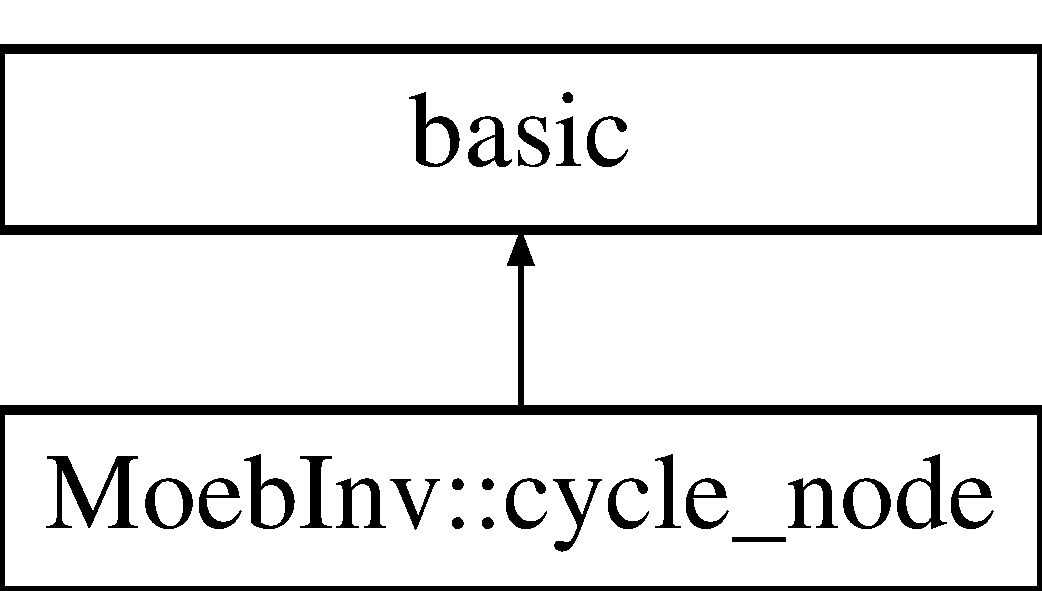
\includegraphics[height=2.000000cm]{class_moeb_inv_1_1cycle__node}
\end{center}
\end{figure}
\subsection*{Public Member Functions}
\begin{DoxyCompactItemize}
\item 
\mbox{\Hypertarget{class_moeb_inv_1_1cycle__node_a0c4a6c987fe260cde30a53073ecd1a67}\label{class_moeb_inv_1_1cycle__node_a0c4a6c987fe260cde30a53073ecd1a67}} 
{\bfseries cycle\+\_\+node} (const ex \&C, int g=0)
\item 
\mbox{\Hypertarget{class_moeb_inv_1_1cycle__node_ad85d4ed7473fc95e446cd7348907aceb}\label{class_moeb_inv_1_1cycle__node_ad85d4ed7473fc95e446cd7348907aceb}} 
{\bfseries cycle\+\_\+node} (const ex \&C, int g, const lst \&par)
\item 
\mbox{\Hypertarget{class_moeb_inv_1_1cycle__node_ac289e7bbafa6ba7507423d9b89cac38f}\label{class_moeb_inv_1_1cycle__node_ac289e7bbafa6ba7507423d9b89cac38f}} 
{\bfseries cycle\+\_\+node} (const ex \&C, int g, const lst \&par, const lst \&chil)
\item 
\mbox{\Hypertarget{class_moeb_inv_1_1cycle__node_a76742aec0d5235ca8c4583421d349f3f}\label{class_moeb_inv_1_1cycle__node_a76742aec0d5235ca8c4583421d349f3f}} 
{\bfseries cycle\+\_\+node} (const ex \&C, int g, const lst \&par, const lst \&chil, string ca)
\item 
\mbox{\Hypertarget{class_moeb_inv_1_1cycle__node_a7a05170989e3dc5698c0f87712b53cf6}\label{class_moeb_inv_1_1cycle__node_a7a05170989e3dc5698c0f87712b53cf6}} 
\mbox{\hyperlink{class_moeb_inv_1_1cycle__node}{cycle\+\_\+node}} {\bfseries subs} (const ex \&e, unsigned options=0) const
\item 
\mbox{\Hypertarget{class_moeb_inv_1_1cycle__node_a2b0c7857d32f39fc292dc192dd35608b}\label{class_moeb_inv_1_1cycle__node_a2b0c7857d32f39fc292dc192dd35608b}} 
void {\bfseries do\+\_\+print\+\_\+double} (const print\+\_\+dflt \&con, unsigned level) const
\item 
\mbox{\Hypertarget{class_moeb_inv_1_1cycle__node_afaf89348492d91a3fbd20ddb65c2663d}\label{class_moeb_inv_1_1cycle__node_afaf89348492d91a3fbd20ddb65c2663d}} 
ex {\bfseries subs} (const exmap \&m, unsigned options=0) const
\end{DoxyCompactItemize}
\subsection*{Protected Member Functions}
\begin{DoxyCompactItemize}
\item 
\mbox{\Hypertarget{class_moeb_inv_1_1cycle__node_ad17e2dddd5252b80cc5350713ea0f07d}\label{class_moeb_inv_1_1cycle__node_ad17e2dddd5252b80cc5350713ea0f07d}} 
void {\bfseries add\+\_\+child} (const ex \&c)
\item 
\mbox{\Hypertarget{class_moeb_inv_1_1cycle__node_a0a09e7f49e1aac1216cbd5d2021716a8}\label{class_moeb_inv_1_1cycle__node_a0a09e7f49e1aac1216cbd5d2021716a8}} 
ex {\bfseries get\+\_\+cycles\+\_\+data} () const
\item 
\mbox{\Hypertarget{class_moeb_inv_1_1cycle__node_a2c6037caa2925d70141552a1bc5ac66c}\label{class_moeb_inv_1_1cycle__node_a2c6037caa2925d70141552a1bc5ac66c}} 
ex {\bfseries make\+\_\+cycles} (const ex \&metr) const
\item 
\mbox{\Hypertarget{class_moeb_inv_1_1cycle__node_a6a95ac1be610f884431348e3574b83ec}\label{class_moeb_inv_1_1cycle__node_a6a95ac1be610f884431348e3574b83ec}} 
ex {\bfseries get\+\_\+cycle\+\_\+data} (int i) const
\item 
\mbox{\Hypertarget{class_moeb_inv_1_1cycle__node_a4cd10d83c284f2e0e800347d4b6cb644}\label{class_moeb_inv_1_1cycle__node_a4cd10d83c284f2e0e800347d4b6cb644}} 
int {\bfseries get\+\_\+generation} () const
\item 
\mbox{\Hypertarget{class_moeb_inv_1_1cycle__node_a6f35e1942b883463f5066b635594f7ab}\label{class_moeb_inv_1_1cycle__node_a6f35e1942b883463f5066b635594f7ab}} 
lst {\bfseries get\+\_\+children} () const
\item 
\mbox{\Hypertarget{class_moeb_inv_1_1cycle__node_abf4b0de955355786912c9c165a9441b9}\label{class_moeb_inv_1_1cycle__node_abf4b0de955355786912c9c165a9441b9}} 
void {\bfseries set\+\_\+cycles} (const ex \&C)
\item 
\mbox{\Hypertarget{class_moeb_inv_1_1cycle__node_add52343eaa8f5614a1b5f99d8b874681}\label{class_moeb_inv_1_1cycle__node_add52343eaa8f5614a1b5f99d8b874681}} 
void {\bfseries append\+\_\+cycle} (const ex \&C)
\item 
\mbox{\Hypertarget{class_moeb_inv_1_1cycle__node_aebf792111a9c9c8e698fe347edf86dd0}\label{class_moeb_inv_1_1cycle__node_aebf792111a9c9c8e698fe347edf86dd0}} 
void {\bfseries append\+\_\+cycle} (const ex \&k, const ex \&l, const ex \&m)
\item 
\mbox{\Hypertarget{class_moeb_inv_1_1cycle__node_a73f295b9f0371810e5bb39433390ee9a}\label{class_moeb_inv_1_1cycle__node_a73f295b9f0371810e5bb39433390ee9a}} 
lst {\bfseries get\+\_\+parents} () const
\item 
\mbox{\Hypertarget{class_moeb_inv_1_1cycle__node_ab27247598c10f8556c3e17b1a0bd8cde}\label{class_moeb_inv_1_1cycle__node_ab27247598c10f8556c3e17b1a0bd8cde}} 
lst {\bfseries get\+\_\+parent\+\_\+keys} () const
\item 
\mbox{\Hypertarget{class_moeb_inv_1_1cycle__node_a265752f76a34351411dbfaac7ec8c1f0}\label{class_moeb_inv_1_1cycle__node_a265752f76a34351411dbfaac7ec8c1f0}} 
void {\bfseries remove\+\_\+child} (const ex \&c)
\item 
\mbox{\Hypertarget{class_moeb_inv_1_1cycle__node_a6112cb6ef1b734d8c04d487c0eb1d1d4}\label{class_moeb_inv_1_1cycle__node_a6112cb6ef1b734d8c04d487c0eb1d1d4}} 
void {\bfseries set\+\_\+asy\+\_\+opt} (const string opt)
\item 
\mbox{\Hypertarget{class_moeb_inv_1_1cycle__node_ac393d7c09b5a3562f94747bf4c08e583}\label{class_moeb_inv_1_1cycle__node_ac393d7c09b5a3562f94747bf4c08e583}} 
string {\bfseries get\+\_\+asy\+\_\+opt} () const
\item 
\mbox{\Hypertarget{class_moeb_inv_1_1cycle__node_a968b7445796d9e39e5e7465b474592cc}\label{class_moeb_inv_1_1cycle__node_a968b7445796d9e39e5e7465b474592cc}} 
size\+\_\+t {\bfseries nops} () const
\item 
\mbox{\Hypertarget{class_moeb_inv_1_1cycle__node_a7e3343b22ec8eb7227c972e3d3e71629}\label{class_moeb_inv_1_1cycle__node_a7e3343b22ec8eb7227c972e3d3e71629}} 
ex {\bfseries op} (size\+\_\+t i) const
\item 
\mbox{\Hypertarget{class_moeb_inv_1_1cycle__node_a29f0d4cb1c6619b47fcb1a0140e4ad6e}\label{class_moeb_inv_1_1cycle__node_a29f0d4cb1c6619b47fcb1a0140e4ad6e}} 
ex \& {\bfseries let\+\_\+op} (size\+\_\+t i)
\item 
\mbox{\Hypertarget{class_moeb_inv_1_1cycle__node_a0e8ec9fed46c1a638806e6bb3b61fbdd}\label{class_moeb_inv_1_1cycle__node_a0e8ec9fed46c1a638806e6bb3b61fbdd}} 
void {\bfseries do\+\_\+print} (const print\+\_\+dflt \&con, unsigned level) const
\item 
\mbox{\Hypertarget{class_moeb_inv_1_1cycle__node_a9fcb6b771522b61b18c702be59d4a7e3}\label{class_moeb_inv_1_1cycle__node_a9fcb6b771522b61b18c702be59d4a7e3}} 
void {\bfseries do\+\_\+print\+\_\+tree} (const print\+\_\+tree \&con, unsigned level) const
\item 
\mbox{\Hypertarget{class_moeb_inv_1_1cycle__node_a83414b9efe3191e16679f5cd91f96125}\label{class_moeb_inv_1_1cycle__node_a83414b9efe3191e16679f5cd91f96125}} 
return\+\_\+type\+\_\+t {\bfseries return\+\_\+type\+\_\+tinfo} () const
\item 
\mbox{\Hypertarget{class_moeb_inv_1_1cycle__node_aed6b7101a72ebe6e7d479fd74420bda2}\label{class_moeb_inv_1_1cycle__node_aed6b7101a72ebe6e7d479fd74420bda2}} 
void {\bfseries archive} (archive\+\_\+node \&n) const
\item 
\mbox{\Hypertarget{class_moeb_inv_1_1cycle__node_af9fd14be29696726f9cd15c0fb106fda}\label{class_moeb_inv_1_1cycle__node_af9fd14be29696726f9cd15c0fb106fda}} 
void {\bfseries read\+\_\+archive} (const archive\+\_\+node \&n, lst \&sym\+\_\+lst)
\end{DoxyCompactItemize}
\subsection*{Protected Attributes}
\begin{DoxyCompactItemize}
\item 
\mbox{\Hypertarget{class_moeb_inv_1_1cycle__node_ae1f5316d67066b275f9c50c6791d2a25}\label{class_moeb_inv_1_1cycle__node_ae1f5316d67066b275f9c50c6791d2a25}} 
lst {\bfseries cycles}
\item 
\mbox{\Hypertarget{class_moeb_inv_1_1cycle__node_a85d78c21e3b9d1225f254d9d726be2dc}\label{class_moeb_inv_1_1cycle__node_a85d78c21e3b9d1225f254d9d726be2dc}} 
int {\bfseries generation}
\item 
\mbox{\Hypertarget{class_moeb_inv_1_1cycle__node_aeea2ab8582613cc50606089bb7c8fed8}\label{class_moeb_inv_1_1cycle__node_aeea2ab8582613cc50606089bb7c8fed8}} 
lst {\bfseries children}
\item 
\mbox{\Hypertarget{class_moeb_inv_1_1cycle__node_ab648167bc5d4d184714e74f494f8acbd}\label{class_moeb_inv_1_1cycle__node_ab648167bc5d4d184714e74f494f8acbd}} 
lst {\bfseries parents}
\item 
\mbox{\Hypertarget{class_moeb_inv_1_1cycle__node_a140cf77b9e0d077cd1ab70f86dc5fc5a}\label{class_moeb_inv_1_1cycle__node_a140cf77b9e0d077cd1ab70f86dc5fc5a}} 
string {\bfseries custom\+\_\+asy}
\end{DoxyCompactItemize}
\subsection*{Friends}
\begin{DoxyCompactItemize}
\item 
\mbox{\Hypertarget{class_moeb_inv_1_1cycle__node_ab77da22cfd9a585b10b4077bd20dafed}\label{class_moeb_inv_1_1cycle__node_ab77da22cfd9a585b10b4077bd20dafed}} 
class {\bfseries cycle\+\_\+relation}
\item 
\mbox{\Hypertarget{class_moeb_inv_1_1cycle__node_ac46ec1ee00928c9cde5b63a7edba7b7a}\label{class_moeb_inv_1_1cycle__node_ac46ec1ee00928c9cde5b63a7edba7b7a}} 
class {\bfseries figure}
\end{DoxyCompactItemize}


The documentation for this class was generated from the following file\+:\begin{DoxyCompactItemize}
\item 
/\+Users/lukehutton/\+One\+Drive -\/ University of Leeds/\+University/\+Computer Science/\+Internship/moebinv-\/gui/lib/moebinv-\/3.\+2/include/figure.\+h\end{DoxyCompactItemize}

\hypertarget{class_moeb_inv_1_1cycle__relation}{}\section{Moeb\+Inv\+:\+:cycle\+\_\+relation Class Reference}
\label{class_moeb_inv_1_1cycle__relation}\index{Moeb\+Inv\+::cycle\+\_\+relation@{Moeb\+Inv\+::cycle\+\_\+relation}}
Inheritance diagram for Moeb\+Inv\+:\+:cycle\+\_\+relation\+:\begin{figure}[H]
\begin{center}
\leavevmode
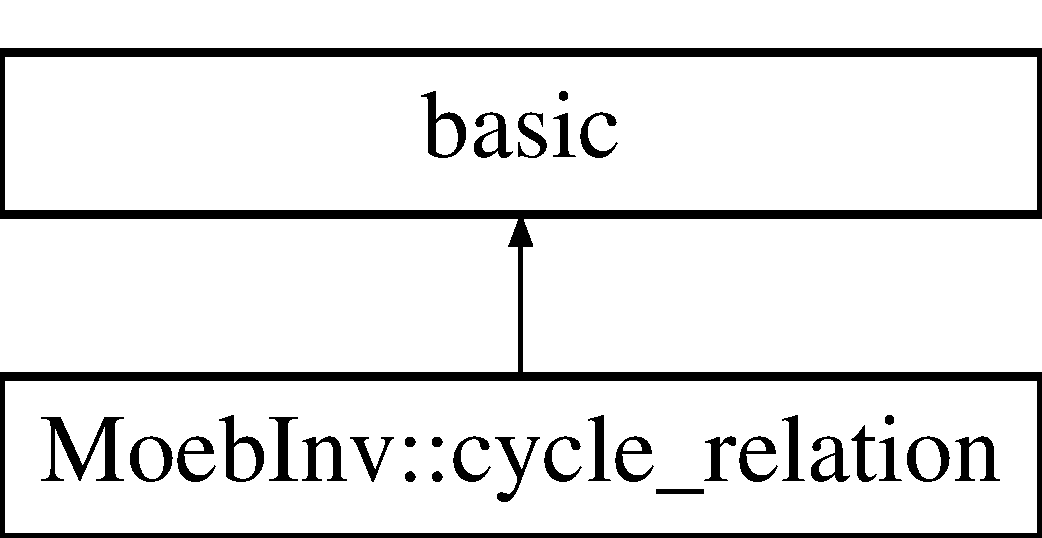
\includegraphics[height=2.000000cm]{class_moeb_inv_1_1cycle__relation}
\end{center}
\end{figure}
\subsection*{Public Member Functions}
\begin{DoxyCompactItemize}
\item 
\mbox{\Hypertarget{class_moeb_inv_1_1cycle__relation_a13d39ba6d4d94b9d33239fd6ac2816cd}\label{class_moeb_inv_1_1cycle__relation_a13d39ba6d4d94b9d33239fd6ac2816cd}} 
{\bfseries cycle\+\_\+relation} (const ex \&key, P\+CR rel, bool cm=true, const ex \&p=0)
\item 
\mbox{\Hypertarget{class_moeb_inv_1_1cycle__relation_a124237c9fdf50d9d7acbf8b8ec06399b}\label{class_moeb_inv_1_1cycle__relation_a124237c9fdf50d9d7acbf8b8ec06399b}} 
ex {\bfseries get\+\_\+parkey} () const
\item 
\mbox{\Hypertarget{class_moeb_inv_1_1cycle__relation_a1e580ad7bc9d962b2adab5d22d8a308b}\label{class_moeb_inv_1_1cycle__relation_a1e580ad7bc9d962b2adab5d22d8a308b}} 
P\+CR {\bfseries get\+\_\+\+P\+CR} () const
\item 
\mbox{\Hypertarget{class_moeb_inv_1_1cycle__relation_a7940baf02b699b5e2cf93d11783b69ae}\label{class_moeb_inv_1_1cycle__relation_a7940baf02b699b5e2cf93d11783b69ae}} 
ex {\bfseries get\+\_\+parameter} () const
\item 
\mbox{\Hypertarget{class_moeb_inv_1_1cycle__relation_a740807052ab3613d29229cdbef0156c3}\label{class_moeb_inv_1_1cycle__relation_a740807052ab3613d29229cdbef0156c3}} 
bool {\bfseries cycle\+\_\+metric\+\_\+inuse} () const
\item 
\mbox{\Hypertarget{class_moeb_inv_1_1cycle__relation_a660797b3b804d3d656f6456b8e6cca8d}\label{class_moeb_inv_1_1cycle__relation_a660797b3b804d3d656f6456b8e6cca8d}} 
ex {\bfseries subs} (const exmap \&em, unsigned options=0) const
\end{DoxyCompactItemize}
\subsection*{Protected Member Functions}
\begin{DoxyCompactItemize}
\item 
\mbox{\Hypertarget{class_moeb_inv_1_1cycle__relation_a9425b2b5b05fa2f701cd9ff769403efe}\label{class_moeb_inv_1_1cycle__relation_a9425b2b5b05fa2f701cd9ff769403efe}} 
ex {\bfseries rel\+\_\+to\+\_\+parent} (const ex \&C1, const ex \&pmetric, const ex \&cmetric, const exhashmap$<$ \mbox{\hyperlink{class_moeb_inv_1_1cycle__node}{cycle\+\_\+node}} $>$ \&N) const
\item 
\mbox{\Hypertarget{class_moeb_inv_1_1cycle__relation_aaba7256a95da266cc70e21ea3a2909bb}\label{class_moeb_inv_1_1cycle__relation_aaba7256a95da266cc70e21ea3a2909bb}} 
return\+\_\+type\+\_\+t {\bfseries return\+\_\+type\+\_\+tinfo} () const
\item 
\mbox{\Hypertarget{class_moeb_inv_1_1cycle__relation_a86492bca17669791dc9ed1a4b4437f70}\label{class_moeb_inv_1_1cycle__relation_a86492bca17669791dc9ed1a4b4437f70}} 
void {\bfseries do\+\_\+print} (const print\+\_\+dflt \&con, unsigned level) const
\item 
\mbox{\Hypertarget{class_moeb_inv_1_1cycle__relation_a601b511cf18754e68c02b090d583f05a}\label{class_moeb_inv_1_1cycle__relation_a601b511cf18754e68c02b090d583f05a}} 
void {\bfseries do\+\_\+print\+\_\+tree} (const print\+\_\+tree \&con, unsigned level) const
\item 
\mbox{\Hypertarget{class_moeb_inv_1_1cycle__relation_aacb68be8d562ef4abd38b97b4bb21198}\label{class_moeb_inv_1_1cycle__relation_aacb68be8d562ef4abd38b97b4bb21198}} 
void {\bfseries archive} (archive\+\_\+node \&n) const
\item 
\mbox{\Hypertarget{class_moeb_inv_1_1cycle__relation_add29cbea61272e7e87ef6e23539fb6a9}\label{class_moeb_inv_1_1cycle__relation_add29cbea61272e7e87ef6e23539fb6a9}} 
void {\bfseries read\+\_\+archive} (const archive\+\_\+node \&n, lst \&sym\+\_\+lst)
\item 
\mbox{\Hypertarget{class_moeb_inv_1_1cycle__relation_a0179243f66e4c3d33278e0687cb2b6e4}\label{class_moeb_inv_1_1cycle__relation_a0179243f66e4c3d33278e0687cb2b6e4}} 
size\+\_\+t {\bfseries nops} () const
\item 
\mbox{\Hypertarget{class_moeb_inv_1_1cycle__relation_afe4e9cb71d813b65194503bafe94dc6b}\label{class_moeb_inv_1_1cycle__relation_afe4e9cb71d813b65194503bafe94dc6b}} 
ex {\bfseries op} (size\+\_\+t i) const
\item 
\mbox{\Hypertarget{class_moeb_inv_1_1cycle__relation_a27c13bcd919ee4b852f7a0a2a4acfb94}\label{class_moeb_inv_1_1cycle__relation_a27c13bcd919ee4b852f7a0a2a4acfb94}} 
ex \& {\bfseries let\+\_\+op} (size\+\_\+t i)
\end{DoxyCompactItemize}
\subsection*{Protected Attributes}
\begin{DoxyCompactItemize}
\item 
\mbox{\Hypertarget{class_moeb_inv_1_1cycle__relation_a7f895ff256fae59239bf1cb075f5b28c}\label{class_moeb_inv_1_1cycle__relation_a7f895ff256fae59239bf1cb075f5b28c}} 
ex {\bfseries parkey}
\item 
\mbox{\Hypertarget{class_moeb_inv_1_1cycle__relation_a720f4183a6c4d0d467b1c1b4d47b60ae}\label{class_moeb_inv_1_1cycle__relation_a720f4183a6c4d0d467b1c1b4d47b60ae}} 
P\+CR {\bfseries rel}
\item 
\mbox{\Hypertarget{class_moeb_inv_1_1cycle__relation_abedf888e85ce0f3eb5f62dfa72c5eb88}\label{class_moeb_inv_1_1cycle__relation_abedf888e85ce0f3eb5f62dfa72c5eb88}} 
ex {\bfseries parameter}
\item 
\mbox{\Hypertarget{class_moeb_inv_1_1cycle__relation_a9afaded728597f76bbbe36cd5ed6de5f}\label{class_moeb_inv_1_1cycle__relation_a9afaded728597f76bbbe36cd5ed6de5f}} 
bool {\bfseries use\+\_\+cycle\+\_\+metric}
\end{DoxyCompactItemize}
\subsection*{Friends}
\begin{DoxyCompactItemize}
\item 
\mbox{\Hypertarget{class_moeb_inv_1_1cycle__relation_ab1135e74268f9c17da7328c07edd8b09}\label{class_moeb_inv_1_1cycle__relation_ab1135e74268f9c17da7328c07edd8b09}} 
class {\bfseries cycle\+\_\+node}
\item 
\mbox{\Hypertarget{class_moeb_inv_1_1cycle__relation_ac46ec1ee00928c9cde5b63a7edba7b7a}\label{class_moeb_inv_1_1cycle__relation_ac46ec1ee00928c9cde5b63a7edba7b7a}} 
class {\bfseries figure}
\end{DoxyCompactItemize}


The documentation for this class was generated from the following file\+:\begin{DoxyCompactItemize}
\item 
/\+Users/lukehutton/\+One\+Drive -\/ University of Leeds/\+University/\+Computer Science/\+Internship/moebinv-\/gui/lib/moebinv-\/3.\+2/include/figure.\+h\end{DoxyCompactItemize}

\hypertarget{classcycle_context_menu}{}\section{cycle\+Context\+Menu Class Reference}
\label{classcycle_context_menu}\index{cycle\+Context\+Menu@{cycle\+Context\+Menu}}


The \mbox{\hyperlink{classcycle_context_menu}{cycle\+Context\+Menu}} class.  




{\ttfamily \#include $<$cyclecontextmenu.\+h$>$}

Inheritance diagram for cycle\+Context\+Menu\+:\begin{figure}[H]
\begin{center}
\leavevmode
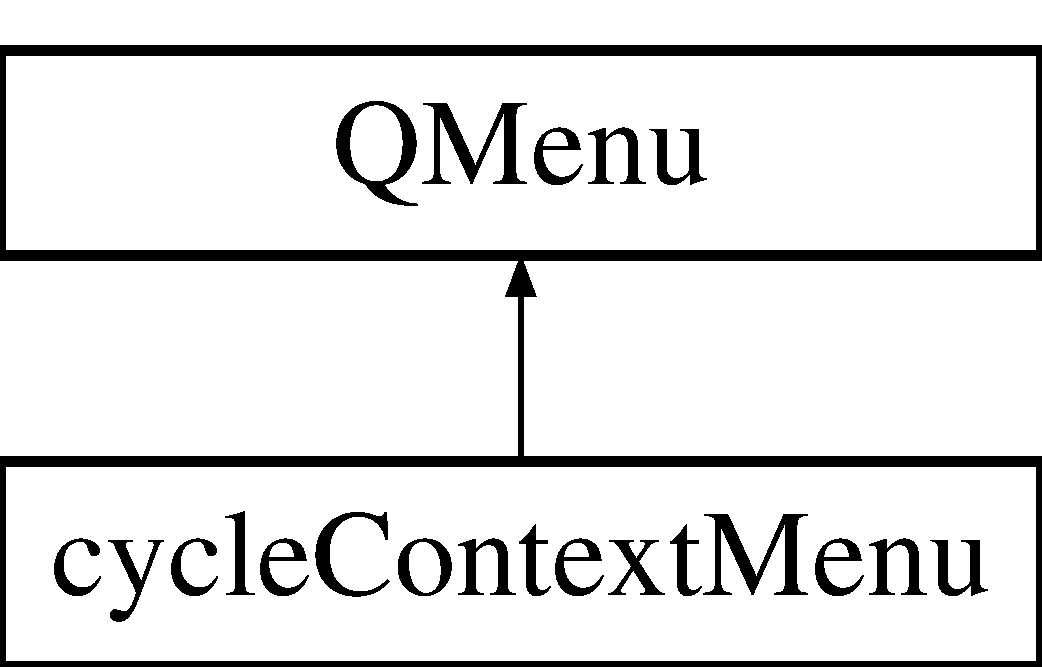
\includegraphics[height=2.000000cm]{classcycle_context_menu}
\end{center}
\end{figure}
\subsection*{Public Slots}
\begin{DoxyCompactItemize}
\item 
\mbox{\Hypertarget{classcycle_context_menu_a844d59a74d643b19fd19eb1de11ea4e9}\label{classcycle_context_menu_a844d59a74d643b19fd19eb1de11ea4e9}} 
void \mbox{\hyperlink{classcycle_context_menu_a844d59a74d643b19fd19eb1de11ea4e9}{confirm\+Delete\+Cycle}} ()
\begin{DoxyCompactList}\small\item\em \mbox{\hyperlink{classcycle_context_menu_a844d59a74d643b19fd19eb1de11ea4e9}{cycle\+Context\+Menu\+::confirm\+Delete\+Cycle}} slot that asks the user whether they would like to delete the cycle. If they select yes the cycle is deleted from the figure and the scene is updated. \end{DoxyCompactList}\item 
\mbox{\Hypertarget{classcycle_context_menu_a6a75f4ba6b3db319468db92fd0948a65}\label{classcycle_context_menu_a6a75f4ba6b3db319468db92fd0948a65}} 
void \mbox{\hyperlink{classcycle_context_menu_a6a75f4ba6b3db319468db92fd0948a65}{amend\+Relation\+List}} ()
\begin{DoxyCompactList}\small\item\em \mbox{\hyperlink{classcycle_context_menu_a6a75f4ba6b3db319468db92fd0948a65}{cycle\+Context\+Menu\+::amend\+Relation\+List}} This slot corrects the relation list after a new relation has been selected. First the sender object is identified. If the sender action is in a group then the whole of the group is searched removing any relations that are not checked (since anyone of them could have been checked before). Then the relation is added to the relation list if it has been checked and removed if it hasn\textquotesingle{}t. The relations\+Have\+Changed signal is emmitted to update the status bar text at the bottom of the application. \end{DoxyCompactList}\item 
\mbox{\Hypertarget{classcycle_context_menu_abf4f98f97561d5acd104a6c0b2038e15}\label{classcycle_context_menu_abf4f98f97561d5acd104a6c0b2038e15}} 
void \mbox{\hyperlink{classcycle_context_menu_abf4f98f97561d5acd104a6c0b2038e15}{display\+Colour\+Dialog}} ()
\begin{DoxyCompactList}\small\item\em \mbox{\hyperlink{classcycle_context_menu_abf4f98f97561d5acd104a6c0b2038e15}{cycle\+Context\+Menu\+::display\+Colour\+Dialog}} Displays the colour dialog so the user can select a colour for the cycle. \end{DoxyCompactList}\item 
\mbox{\Hypertarget{classcycle_context_menu_a094bbed14bab12e3b9ac3ae07140bdcb}\label{classcycle_context_menu_a094bbed14bab12e3b9ac3ae07140bdcb}} 
void \mbox{\hyperlink{classcycle_context_menu_a094bbed14bab12e3b9ac3ae07140bdcb}{display\+Style\+Dialog}} ()
\begin{DoxyCompactList}\small\item\em \mbox{\hyperlink{classcycle_context_menu_a094bbed14bab12e3b9ac3ae07140bdcb}{cycle\+Context\+Menu\+::display\+Style\+Dialog}} Display the style dialog so the user can select a style for the cycle. \end{DoxyCompactList}\item 
\mbox{\Hypertarget{classcycle_context_menu_ac720f89ffd13952e79dd77c1bb15c2aa}\label{classcycle_context_menu_ac720f89ffd13952e79dd77c1bb15c2aa}} 
void \mbox{\hyperlink{classcycle_context_menu_ac720f89ffd13952e79dd77c1bb15c2aa}{display\+Weight\+Dialog}} ()
\begin{DoxyCompactList}\small\item\em \mbox{\hyperlink{classcycle_context_menu_ac720f89ffd13952e79dd77c1bb15c2aa}{cycle\+Context\+Menu\+::display\+Weight\+Dialog}} Display the weight dialog so the user can select a weight for the cycle. \end{DoxyCompactList}\item 
void \mbox{\hyperlink{classcycle_context_menu_ae807f1cddefcdedf9f8c60473bd287df}{edit\+Point}} ()
\begin{DoxyCompactList}\small\item\em \mbox{\hyperlink{classcycle_context_menu_ae807f1cddefcdedf9f8c60473bd287df}{cycle\+Context\+Menu\+::edit\+Point}} \end{DoxyCompactList}\end{DoxyCompactItemize}
\subsection*{Signals}
\begin{DoxyCompactItemize}
\item 
\mbox{\Hypertarget{classcycle_context_menu_a42d360ffa2a047c3f43ded9fcec5982b}\label{classcycle_context_menu_a42d360ffa2a047c3f43ded9fcec5982b}} 
void {\bfseries relations\+Have\+Changed} ()
\item 
\mbox{\Hypertarget{classcycle_context_menu_acd8ba953b7b1edfac94b5ba4158217af}\label{classcycle_context_menu_acd8ba953b7b1edfac94b5ba4158217af}} 
void {\bfseries colour\+Selected} (Q\+Color colour)
\item 
\mbox{\Hypertarget{classcycle_context_menu_ac91d09b750dfeace9334b67649fbbda0}\label{classcycle_context_menu_ac91d09b750dfeace9334b67649fbbda0}} 
void {\bfseries weight\+Selected} (double weight)
\item 
\mbox{\Hypertarget{classcycle_context_menu_a31b1b2e1f6596697cdac2cf0cb66359e}\label{classcycle_context_menu_a31b1b2e1f6596697cdac2cf0cb66359e}} 
void {\bfseries style\+Selected} (int style)
\item 
\mbox{\Hypertarget{classcycle_context_menu_a0e28f14e9918aef074523854b5364c3e}\label{classcycle_context_menu_a0e28f14e9918aef074523854b5364c3e}} 
void {\bfseries scene\+Invalid} ()
\item 
\mbox{\Hypertarget{classcycle_context_menu_a6b92c1d84f101c8386d1152b680247ff}\label{classcycle_context_menu_a6b92c1d84f101c8386d1152b680247ff}} 
void {\bfseries changes\+Made\+To\+Figure} (const Moeb\+Inv\+::figure \&original\+Figure, const Moeb\+Inv\+::figure \&changed\+Figure)
\end{DoxyCompactItemize}
\subsection*{Public Member Functions}
\begin{DoxyCompactItemize}
\item 
\mbox{\hyperlink{classcycle_context_menu_a0a948765494ab4b2ecf73c89123f7f14}{cycle\+Context\+Menu}} (Moeb\+Inv\+::figure $\ast$f, Gi\+Na\+C\+::ex cycle, Gi\+Na\+C\+::lst $\ast$relation\+List, bool is\+Delete=true, bool is\+This=false, bool show\+Edit\+Menu=false)
\begin{DoxyCompactList}\small\item\em \mbox{\hyperlink{classcycle_context_menu_a0a948765494ab4b2ecf73c89123f7f14}{cycle\+Context\+Menu\+::cycle\+Context\+Menu}} Context menu constructor \end{DoxyCompactList}\item 
Gi\+Na\+C\+::ex \mbox{\hyperlink{classcycle_context_menu_a35b3868cdc32b97e7c4abc109ee13460}{get\+Cycle}} ()
\begin{DoxyCompactList}\small\item\em \mbox{\hyperlink{classcycle_context_menu_a35b3868cdc32b97e7c4abc109ee13460}{cycle\+Context\+Menu\+::get\+Cycle}} get cycle related to the context menu. \end{DoxyCompactList}\item 
Q\+List$<$ \mbox{\hyperlink{classmenu_rel_action}{menu\+Rel\+Action}} $\ast$ $>$ \mbox{\hyperlink{classcycle_context_menu_a4dd57e4522c46a70367b6b721f23bcc9}{get\+Actions}} ()
\begin{DoxyCompactList}\small\item\em \mbox{\hyperlink{classcycle_context_menu_a4dd57e4522c46a70367b6b721f23bcc9}{cycle\+Context\+Menu\+::get\+Actions}} get actions in the context menu. \end{DoxyCompactList}\item 
Q\+Action $\ast$ \mbox{\hyperlink{classcycle_context_menu_a0e955d1a633d3585d11b7c193341a568}{get\+Title\+Action}} ()
\begin{DoxyCompactList}\small\item\em \mbox{\hyperlink{classcycle_context_menu_a0e955d1a633d3585d11b7c193341a568}{cycle\+Context\+Menu\+::get\+Title\+Action}} get the action that will be used as the title of the context menu. This has been created due to the fact that cross compatability for \textquotesingle{}add\+Section()\textquotesingle{} isn\textquotesingle{}t well established. \end{DoxyCompactList}\item 
void \mbox{\hyperlink{classcycle_context_menu_adf29caf51604118b6ced6a02c5172252}{set\+Cycle}} (Gi\+Na\+C\+::ex cycle)
\begin{DoxyCompactList}\small\item\em \mbox{\hyperlink{classcycle_context_menu_adf29caf51604118b6ced6a02c5172252}{cycle\+Context\+Menu\+::set\+Cycle}} set the cycle that the context menu represents. \end{DoxyCompactList}\item 
void \mbox{\hyperlink{classcycle_context_menu_a83f3eb1ea5338154095a7bf1e2c77b01}{remove\+Relation\+From\+List}} (\mbox{\hyperlink{classmenu_rel_action}{menu\+Rel\+Action}} $\ast$action\+Triggered)
\begin{DoxyCompactList}\small\item\em \mbox{\hyperlink{classcycle_context_menu_a83f3eb1ea5338154095a7bf1e2c77b01}{cycle\+Context\+Menu\+::remove\+Relation\+From\+List}} This function removes a relation from the list by creating a new list and adding every item except the item that needs to be removed. The \textquotesingle{}relation\+List\textquotesingle{} from \mbox{\hyperlink{class_main_window}{Main\+Window}} is then updated so that \textquotesingle{}relation\textquotesingle{} is no longer in the list. \end{DoxyCompactList}\item 
void \mbox{\hyperlink{classcycle_context_menu_a155448ae220555423d26b055f50b6e49}{build\+Context\+Menu}} ()
\begin{DoxyCompactList}\small\item\em \mbox{\hyperlink{classcycle_context_menu_a155448ae220555423d26b055f50b6e49}{cycle\+Context\+Menu\+::build\+Context\+Menu}} Build the layout of the contextmenu. \end{DoxyCompactList}\item 
\mbox{\Hypertarget{classcycle_context_menu_a2ada1b40956db90398503d184afdd5ee}\label{classcycle_context_menu_a2ada1b40956db90398503d184afdd5ee}} 
void \mbox{\hyperlink{classcycle_context_menu_a2ada1b40956db90398503d184afdd5ee}{build\+Actions}} ()
\begin{DoxyCompactList}\small\item\em \mbox{\hyperlink{classcycle_context_menu_a2ada1b40956db90398503d184afdd5ee}{cycle\+Context\+Menu\+::build\+Actions}} initialize all the actions that will be displayed in the context menu and connect their trigger signals to slots. \end{DoxyCompactList}\item 
\mbox{\Hypertarget{classcycle_context_menu_a17d519c784fac28e39da31478b810ae9}\label{classcycle_context_menu_a17d519c784fac28e39da31478b810ae9}} 
Q\+String {\bfseries node\+\_\+label} (Gi\+Na\+C\+::ex name)
\end{DoxyCompactItemize}
\subsection*{Public Attributes}
\begin{DoxyCompactItemize}
\item 
\mbox{\Hypertarget{classcycle_context_menu_a1e2215915914b4c36463cbe5e667722d}\label{classcycle_context_menu_a1e2215915914b4c36463cbe5e667722d}} 
Q\+Pointer$<$ Q\+Action $>$ {\bfseries change\+Colour} = nullptr
\item 
\mbox{\Hypertarget{classcycle_context_menu_a61f2889cd624664ec0b4933def974a04}\label{classcycle_context_menu_a61f2889cd624664ec0b4933def974a04}} 
Q\+Pointer$<$ Q\+Action $>$ {\bfseries change\+Style} = nullptr
\item 
\mbox{\Hypertarget{classcycle_context_menu_a9798e2ec98b4e15af313112411cd8a24}\label{classcycle_context_menu_a9798e2ec98b4e15af313112411cd8a24}} 
Q\+Pointer$<$ Q\+Action $>$ {\bfseries change\+Weight} = nullptr
\item 
\mbox{\Hypertarget{classcycle_context_menu_aa58c68008bb6ab0d70af517821b8a48f}\label{classcycle_context_menu_aa58c68008bb6ab0d70af517821b8a48f}} 
Q\+Pointer$<$ Q\+Action $>$ {\bfseries delete\+Point} = nullptr
\item 
\mbox{\Hypertarget{classcycle_context_menu_a7c9b8d13930dc91c050e5b870f7dbfb8}\label{classcycle_context_menu_a7c9b8d13930dc91c050e5b870f7dbfb8}} 
Q\+Pointer$<$ Q\+Action $>$ {\bfseries edit} = nullptr
\end{DoxyCompactItemize}


\subsection{Detailed Description}
The \mbox{\hyperlink{classcycle_context_menu}{cycle\+Context\+Menu}} class. 

This class creates a context menu which is then used by each of the cycles created on the scene. It then connects each of the menu items so they function as intended. 

\subsection{Constructor \& Destructor Documentation}
\mbox{\Hypertarget{classcycle_context_menu_a0a948765494ab4b2ecf73c89123f7f14}\label{classcycle_context_menu_a0a948765494ab4b2ecf73c89123f7f14}} 
\index{cycle\+Context\+Menu@{cycle\+Context\+Menu}!cycle\+Context\+Menu@{cycle\+Context\+Menu}}
\index{cycle\+Context\+Menu@{cycle\+Context\+Menu}!cycle\+Context\+Menu@{cycle\+Context\+Menu}}
\subsubsection{\texorpdfstring{cycle\+Context\+Menu()}{cycleContextMenu()}}
{\footnotesize\ttfamily cycle\+Context\+Menu\+::cycle\+Context\+Menu (\begin{DoxyParamCaption}\item[{Moeb\+Inv\+::figure $\ast$}]{f,  }\item[{Gi\+Na\+C\+::ex}]{cycle,  }\item[{Gi\+Na\+C\+::lst $\ast$}]{relation\+List,  }\item[{bool}]{is\+Delete = {\ttfamily true},  }\item[{bool}]{is\+This = {\ttfamily false},  }\item[{bool}]{show\+Edit\+Menu = {\ttfamily false} }\end{DoxyParamCaption})}



\mbox{\hyperlink{classcycle_context_menu_a0a948765494ab4b2ecf73c89123f7f14}{cycle\+Context\+Menu\+::cycle\+Context\+Menu}} Context menu constructor 


\begin{DoxyParams}{Parameters}
{\em f} & -\/ pointer to the figure. \\
\hline
{\em cycle} & -\/ cycle the context menu is related to. \\
\hline
{\em relation\+List} & -\/ pointer to the list that stores the current selected relations from every cycle in the figure. \\
\hline
{\em is\+Delete} & -\/ does the cycle have the delete option or not? (some cycles cannot be deleted e.\+g. infy)\\
\hline
\end{DoxyParams}
Creates a cycle context menu. This allows for the selection and input of relations and allows the properties of a relation to be changed.

\subsubsection*{Current context menu\+: }

\subsubsection*{title }

standard \subsubsection*{relations }

exclusive \subsubsection*{tangent }

relations \subsubsection*{with inputs }

\subsubsection*{style }

\subsubsection*{edit }

\subsubsection*{delete }

\subsection{Member Function Documentation}
\mbox{\Hypertarget{classcycle_context_menu_a155448ae220555423d26b055f50b6e49}\label{classcycle_context_menu_a155448ae220555423d26b055f50b6e49}} 
\index{cycle\+Context\+Menu@{cycle\+Context\+Menu}!build\+Context\+Menu@{build\+Context\+Menu}}
\index{build\+Context\+Menu@{build\+Context\+Menu}!cycle\+Context\+Menu@{cycle\+Context\+Menu}}
\subsubsection{\texorpdfstring{build\+Context\+Menu()}{buildContextMenu()}}
{\footnotesize\ttfamily void cycle\+Context\+Menu\+::build\+Context\+Menu (\begin{DoxyParamCaption}{ }\end{DoxyParamCaption})}



\mbox{\hyperlink{classcycle_context_menu_a155448ae220555423d26b055f50b6e49}{cycle\+Context\+Menu\+::build\+Context\+Menu}} Build the layout of the contextmenu. 

Note\+: If a new relation or action is added this layout function will need to be adapted to suit the new layout. \mbox{\Hypertarget{classcycle_context_menu_ae807f1cddefcdedf9f8c60473bd287df}\label{classcycle_context_menu_ae807f1cddefcdedf9f8c60473bd287df}} 
\index{cycle\+Context\+Menu@{cycle\+Context\+Menu}!edit\+Point@{edit\+Point}}
\index{edit\+Point@{edit\+Point}!cycle\+Context\+Menu@{cycle\+Context\+Menu}}
\subsubsection{\texorpdfstring{edit\+Point}{editPoint}}
{\footnotesize\ttfamily void cycle\+Context\+Menu\+::edit\+Point (\begin{DoxyParamCaption}{ }\end{DoxyParamCaption})\hspace{0.3cm}{\ttfamily [slot]}}



\mbox{\hyperlink{classcycle_context_menu_ae807f1cddefcdedf9f8c60473bd287df}{cycle\+Context\+Menu\+::edit\+Point}} 

Displays a dialog that allows you to edit a point of generation 0. This dialog lets you enter the values k, l, n, m or (x, y) and radius squared to edit a point. \mbox{\Hypertarget{classcycle_context_menu_a4dd57e4522c46a70367b6b721f23bcc9}\label{classcycle_context_menu_a4dd57e4522c46a70367b6b721f23bcc9}} 
\index{cycle\+Context\+Menu@{cycle\+Context\+Menu}!get\+Actions@{get\+Actions}}
\index{get\+Actions@{get\+Actions}!cycle\+Context\+Menu@{cycle\+Context\+Menu}}
\subsubsection{\texorpdfstring{get\+Actions()}{getActions()}}
{\footnotesize\ttfamily Q\+List$<$ \mbox{\hyperlink{classmenu_rel_action}{menu\+Rel\+Action}} $\ast$ $>$ cycle\+Context\+Menu\+::get\+Actions (\begin{DoxyParamCaption}{ }\end{DoxyParamCaption})}



\mbox{\hyperlink{classcycle_context_menu_a4dd57e4522c46a70367b6b721f23bcc9}{cycle\+Context\+Menu\+::get\+Actions}} get actions in the context menu. 

\begin{DoxyReturn}{Returns}
Q\+List$<$menu\+Rel\+Action $\ast$$>$ list of \mbox{\hyperlink{classmenu_rel_action}{menu\+Rel\+Action}} pointers. 
\end{DoxyReturn}
\mbox{\Hypertarget{classcycle_context_menu_a35b3868cdc32b97e7c4abc109ee13460}\label{classcycle_context_menu_a35b3868cdc32b97e7c4abc109ee13460}} 
\index{cycle\+Context\+Menu@{cycle\+Context\+Menu}!get\+Cycle@{get\+Cycle}}
\index{get\+Cycle@{get\+Cycle}!cycle\+Context\+Menu@{cycle\+Context\+Menu}}
\subsubsection{\texorpdfstring{get\+Cycle()}{getCycle()}}
{\footnotesize\ttfamily ex cycle\+Context\+Menu\+::get\+Cycle (\begin{DoxyParamCaption}{ }\end{DoxyParamCaption})}



\mbox{\hyperlink{classcycle_context_menu_a35b3868cdc32b97e7c4abc109ee13460}{cycle\+Context\+Menu\+::get\+Cycle}} get cycle related to the context menu. 

\begin{DoxyReturn}{Returns}
Gi\+Na\+C\+::ex. 
\end{DoxyReturn}
\mbox{\Hypertarget{classcycle_context_menu_a0e955d1a633d3585d11b7c193341a568}\label{classcycle_context_menu_a0e955d1a633d3585d11b7c193341a568}} 
\index{cycle\+Context\+Menu@{cycle\+Context\+Menu}!get\+Title\+Action@{get\+Title\+Action}}
\index{get\+Title\+Action@{get\+Title\+Action}!cycle\+Context\+Menu@{cycle\+Context\+Menu}}
\subsubsection{\texorpdfstring{get\+Title\+Action()}{getTitleAction()}}
{\footnotesize\ttfamily Q\+Action $\ast$ cycle\+Context\+Menu\+::get\+Title\+Action (\begin{DoxyParamCaption}{ }\end{DoxyParamCaption})}



\mbox{\hyperlink{classcycle_context_menu_a0e955d1a633d3585d11b7c193341a568}{cycle\+Context\+Menu\+::get\+Title\+Action}} get the action that will be used as the title of the context menu. This has been created due to the fact that cross compatability for \textquotesingle{}add\+Section()\textquotesingle{} isn\textquotesingle{}t well established. 

\begin{DoxyReturn}{Returns}
Q\+Action$\ast$ -\/ A pointer to the Q\+Action. 
\end{DoxyReturn}
\mbox{\Hypertarget{classcycle_context_menu_a83f3eb1ea5338154095a7bf1e2c77b01}\label{classcycle_context_menu_a83f3eb1ea5338154095a7bf1e2c77b01}} 
\index{cycle\+Context\+Menu@{cycle\+Context\+Menu}!remove\+Relation\+From\+List@{remove\+Relation\+From\+List}}
\index{remove\+Relation\+From\+List@{remove\+Relation\+From\+List}!cycle\+Context\+Menu@{cycle\+Context\+Menu}}
\subsubsection{\texorpdfstring{remove\+Relation\+From\+List()}{removeRelationFromList()}}
{\footnotesize\ttfamily void cycle\+Context\+Menu\+::remove\+Relation\+From\+List (\begin{DoxyParamCaption}\item[{\mbox{\hyperlink{classmenu_rel_action}{menu\+Rel\+Action}} $\ast$}]{action\+Triggered }\end{DoxyParamCaption})}



\mbox{\hyperlink{classcycle_context_menu_a83f3eb1ea5338154095a7bf1e2c77b01}{cycle\+Context\+Menu\+::remove\+Relation\+From\+List}} This function removes a relation from the list by creating a new list and adding every item except the item that needs to be removed. The \textquotesingle{}relation\+List\textquotesingle{} from \mbox{\hyperlink{class_main_window}{Main\+Window}} is then updated so that \textquotesingle{}relation\textquotesingle{} is no longer in the list. 


\begin{DoxyParams}{Parameters}
{\em relation} & -\/ the cycle\+\_\+relation that is to be removed. \\
\hline
\end{DoxyParams}
\mbox{\Hypertarget{classcycle_context_menu_adf29caf51604118b6ced6a02c5172252}\label{classcycle_context_menu_adf29caf51604118b6ced6a02c5172252}} 
\index{cycle\+Context\+Menu@{cycle\+Context\+Menu}!set\+Cycle@{set\+Cycle}}
\index{set\+Cycle@{set\+Cycle}!cycle\+Context\+Menu@{cycle\+Context\+Menu}}
\subsubsection{\texorpdfstring{set\+Cycle()}{setCycle()}}
{\footnotesize\ttfamily void cycle\+Context\+Menu\+::set\+Cycle (\begin{DoxyParamCaption}\item[{Gi\+Na\+C\+::ex}]{cycle }\end{DoxyParamCaption})}



\mbox{\hyperlink{classcycle_context_menu_adf29caf51604118b6ced6a02c5172252}{cycle\+Context\+Menu\+::set\+Cycle}} set the cycle that the context menu represents. 


\begin{DoxyParams}{Parameters}
{\em cycle} & -\/ the cycle in which the context menu will be \textquotesingle{}linked\textquotesingle{} to. \\
\hline
\end{DoxyParams}


The documentation for this class was generated from the following files\+:\begin{DoxyCompactItemize}
\item 
/\+Users/lukehutton/\+One\+Drive -\/ University of Leeds/\+University/\+Computer Science/\+Internship/moebinv-\/gui/include/cyclecontextmenu.\+h\item 
/\+Users/lukehutton/\+One\+Drive -\/ University of Leeds/\+University/\+Computer Science/\+Internship/moebinv-\/gui/src/cyclecontextmenu.\+cpp\end{DoxyCompactItemize}

\hypertarget{structcycle_data}{}\section{cycle\+Data Struct Reference}
\label{structcycle_data}\index{cycle\+Data@{cycle\+Data}}


The \mbox{\hyperlink{structcycle_data}{cycle\+Data}} struct.  




{\ttfamily \#include $<$graphiccycle.\+h$>$}

\subsection*{Public Attributes}
\begin{DoxyCompactItemize}
\item 
\mbox{\Hypertarget{structcycle_data_a5196a89f9438dfe6aeca79b20b1365dc}\label{structcycle_data_a5196a89f9438dfe6aeca79b20b1365dc}} 
double {\bfseries x}
\item 
\mbox{\Hypertarget{structcycle_data_a943d9aa23035ec42edfaf4f2c6d57095}\label{structcycle_data_a943d9aa23035ec42edfaf4f2c6d57095}} 
double {\bfseries y}
\item 
\mbox{\Hypertarget{structcycle_data_a696c13341d3fee420edacff5630ff797}\label{structcycle_data_a696c13341d3fee420edacff5630ff797}} 
double {\bfseries c}
\item 
\mbox{\Hypertarget{structcycle_data_a815e7bc546bb425f638be27cb805315d}\label{structcycle_data_a815e7bc546bb425f638be27cb805315d}} 
double {\bfseries radius}
\item 
\mbox{\Hypertarget{structcycle_data_aea3d22bf8556ff483f19a00ffa646a13}\label{structcycle_data_aea3d22bf8556ff483f19a00ffa646a13}} 
Q\+Brush $\ast$ {\bfseries brush}
\item 
\mbox{\Hypertarget{structcycle_data_a90e5dc6feb2c6486251d339394810d9b}\label{structcycle_data_a90e5dc6feb2c6486251d339394810d9b}} 
Q\+Pen $\ast$ {\bfseries pen}
\end{DoxyCompactItemize}


\subsection{Detailed Description}
The \mbox{\hyperlink{structcycle_data}{cycle\+Data}} struct. 

Cycle data that each child object needs. 

The documentation for this struct was generated from the following file\+:\begin{DoxyCompactItemize}
\item 
/\+Users/lukehutton/\+One\+Drive -\/ University of Leeds/\+University/\+Computer Science/\+Internship/moebinv-\/gui/include/graphiccycle.\+h\end{DoxyCompactItemize}

\hypertarget{structcycle_style_data}{}\section{cycle\+Style\+Data Struct Reference}
\label{structcycle_style_data}\index{cycle\+Style\+Data@{cycle\+Style\+Data}}
\subsection*{Public Attributes}
\begin{DoxyCompactItemize}
\item 
\mbox{\Hypertarget{structcycle_style_data_a2f0a7ba93c9cb8104399a0357f98507d}\label{structcycle_style_data_a2f0a7ba93c9cb8104399a0357f98507d}} 
bool {\bfseries is\+Default}
\item 
\mbox{\Hypertarget{structcycle_style_data_a77370c35742330617cccebfb0774edcd}\label{structcycle_style_data_a77370c35742330617cccebfb0774edcd}} 
Q\+Color {\bfseries colour}
\item 
\mbox{\Hypertarget{structcycle_style_data_a65843c85926f1ae36e123789026bb09b}\label{structcycle_style_data_a65843c85926f1ae36e123789026bb09b}} 
double {\bfseries line\+Width}
\item 
\mbox{\Hypertarget{structcycle_style_data_a3ff1e430f3bb40585365c496c1702f92}\label{structcycle_style_data_a3ff1e430f3bb40585365c496c1702f92}} 
int {\bfseries line\+Style}
\end{DoxyCompactItemize}


The documentation for this struct was generated from the following file\+:\begin{DoxyCompactItemize}
\item 
/\+Users/lukehutton/\+One\+Drive -\/ University of Leeds/\+University/\+Computer Science/\+Internship/moebinv-\/gui/include/conf.\+h\end{DoxyCompactItemize}

\hypertarget{classdefine_cycle_dialog}{}\section{define\+Cycle\+Dialog Class Reference}
\label{classdefine_cycle_dialog}\index{define\+Cycle\+Dialog@{define\+Cycle\+Dialog}}
Inheritance diagram for define\+Cycle\+Dialog\+:\begin{figure}[H]
\begin{center}
\leavevmode
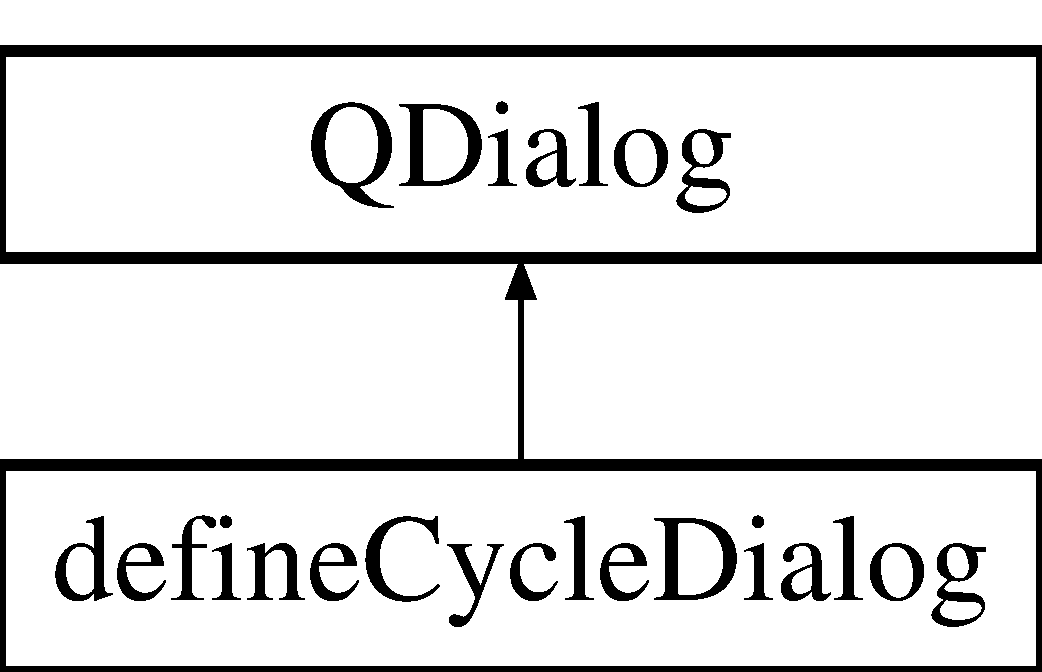
\includegraphics[height=2.000000cm]{classdefine_cycle_dialog}
\end{center}
\end{figure}
\subsection*{Public Member Functions}
\begin{DoxyCompactItemize}
\item 
\mbox{\Hypertarget{classdefine_cycle_dialog_a6f67cfc93b51c9407286019f5f005a22}\label{classdefine_cycle_dialog_a6f67cfc93b51c9407286019f5f005a22}} 
{\bfseries define\+Cycle\+Dialog} (Q\+Widget $\ast$parent=0)
\item 
\mbox{\Hypertarget{classdefine_cycle_dialog_a1839a7fbd4d70faf3f7dbd281ab5d52b}\label{classdefine_cycle_dialog_a1839a7fbd4d70faf3f7dbd281ab5d52b}} 
void {\bfseries set\+Tab} (int index)
\item 
\mbox{\Hypertarget{classdefine_cycle_dialog_aafd97025d92beedcac5c626aab88a6af}\label{classdefine_cycle_dialog_aafd97025d92beedcac5c626aab88a6af}} 
Gi\+Na\+C\+::lst {\bfseries get\+Values} ()
\item 
\mbox{\Hypertarget{classdefine_cycle_dialog_a1725401652da06b5fbc0eef513e2b1d1}\label{classdefine_cycle_dialog_a1725401652da06b5fbc0eef513e2b1d1}} 
void {\bfseries load\+Values} (const Gi\+Na\+C\+::lst \&values)
\end{DoxyCompactItemize}


The documentation for this class was generated from the following files\+:\begin{DoxyCompactItemize}
\item 
/\+Users/lukehutton/\+One\+Drive -\/ University of Leeds/\+University/\+Computer Science/\+Internship/moebinv-\/gui/include/definecycledialog.\+h\item 
/\+Users/lukehutton/\+One\+Drive -\/ University of Leeds/\+University/\+Computer Science/\+Internship/moebinv-\/gui/src/definecycledialog.\+cpp\end{DoxyCompactItemize}

\hypertarget{class_ui_1_1define_cycle_dialog}{}\section{Ui\+:\+:define\+Cycle\+Dialog Class Reference}
\label{class_ui_1_1define_cycle_dialog}\index{Ui\+::define\+Cycle\+Dialog@{Ui\+::define\+Cycle\+Dialog}}
Inheritance diagram for Ui\+:\+:define\+Cycle\+Dialog\+:\begin{figure}[H]
\begin{center}
\leavevmode
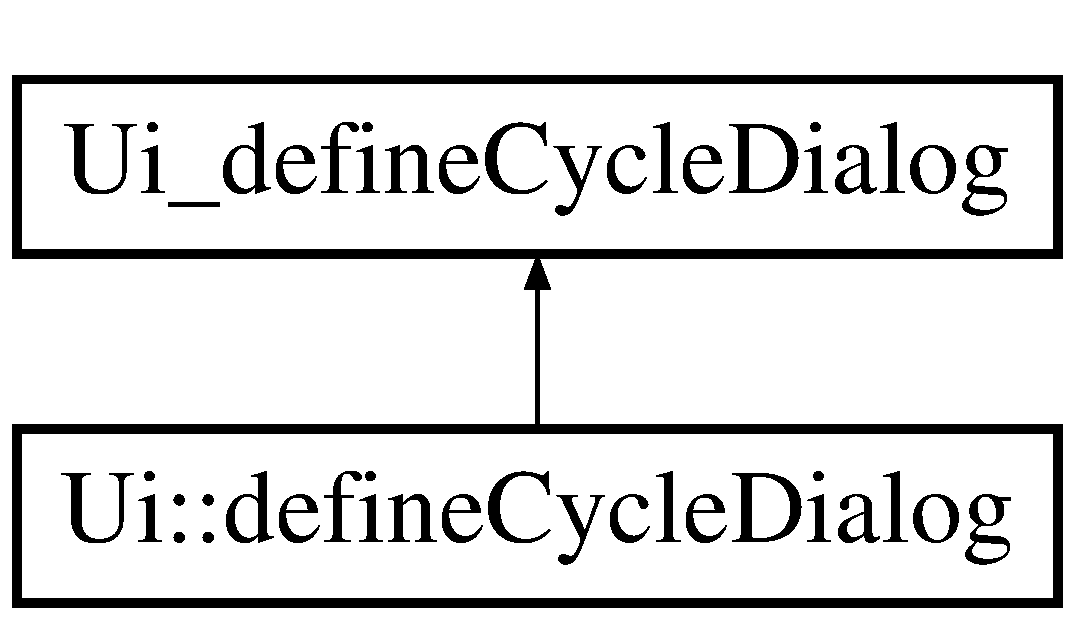
\includegraphics[height=2.000000cm]{class_ui_1_1define_cycle_dialog}
\end{center}
\end{figure}
\subsection*{Additional Inherited Members}


The documentation for this class was generated from the following file\+:\begin{DoxyCompactItemize}
\item 
/\+Users/lukehutton/\+One\+Drive -\/ University of Leeds/\+University/\+Computer Science/\+Internship/moebinv-\/gui/moebinv-\/gui-\/build/ui\+\_\+definecycledialog.\+h\end{DoxyCompactItemize}

\hypertarget{classdock_widget}{}\section{dock\+Widget Class Reference}
\label{classdock_widget}\index{dock\+Widget@{dock\+Widget}}
Inheritance diagram for dock\+Widget\+:\begin{figure}[H]
\begin{center}
\leavevmode
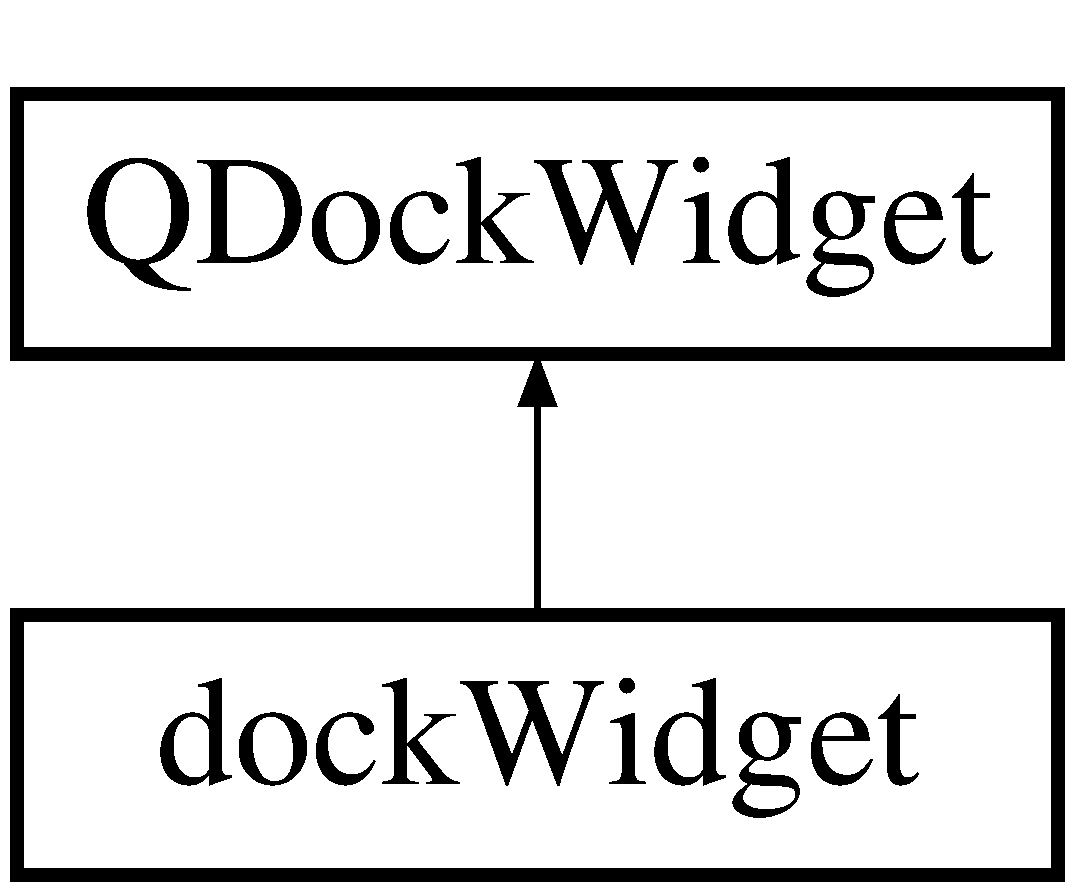
\includegraphics[height=2.000000cm]{classdock_widget}
\end{center}
\end{figure}
\subsection*{Signals}
\begin{DoxyCompactItemize}
\item 
\mbox{\Hypertarget{classdock_widget_acc2d0ff853683454fab7e90e1c772540}\label{classdock_widget_acc2d0ff853683454fab7e90e1c772540}} 
void {\bfseries recenter\+View} ()
\item 
\mbox{\Hypertarget{classdock_widget_a9204c64451a6cf19229c1d93b289f24e}\label{classdock_widget_a9204c64451a6cf19229c1d93b289f24e}} 
void {\bfseries calculate\+Dock\+To\+Window\+Percentage} ()
\end{DoxyCompactItemize}
\subsection*{Public Member Functions}
\begin{DoxyCompactItemize}
\item 
\mbox{\hyperlink{classdock_widget_af65ba19ef794133fb2b365dedc5b9d64}{dock\+Widget}} (Q\+Object $\ast$parent=0)
\begin{DoxyCompactList}\small\item\em \mbox{\hyperlink{classdock_widget_af65ba19ef794133fb2b365dedc5b9d64}{dock\+Widget\+::dock\+Widget}} create a new dock widget with a predetermined size. \end{DoxyCompactList}\item 
void \mbox{\hyperlink{classdock_widget_ae9cc3b91f10ee2af70fd74c6422848b6}{resize\+Event}} (Q\+Resize\+Event $\ast$event)
\begin{DoxyCompactList}\small\item\em \mbox{\hyperlink{classdock_widget_ae9cc3b91f10ee2af70fd74c6422848b6}{dock\+Widget\+::resize\+Event}} triggered on resize event. \end{DoxyCompactList}\item 
void \mbox{\hyperlink{classdock_widget_a7f6a50274259d918d9a9068b8a94fe80}{set\+Size\+Ratio}} (double size\+Ratio)
\begin{DoxyCompactList}\small\item\em \mbox{\hyperlink{classdock_widget_a7f6a50274259d918d9a9068b8a94fe80}{dock\+Widget\+::set\+Size\+Ratio}} sets the size of the dock widget. \end{DoxyCompactList}\item 
double \mbox{\hyperlink{classdock_widget_a2503861f92eb0ac30313dd713f398996}{get\+Size\+Ratio}} ()
\begin{DoxyCompactList}\small\item\em \mbox{\hyperlink{classdock_widget_a2503861f92eb0ac30313dd713f398996}{dock\+Widget\+::get\+Size\+Ratio}} getter for size ratio. \end{DoxyCompactList}\end{DoxyCompactItemize}


\subsection{Constructor \& Destructor Documentation}
\mbox{\Hypertarget{classdock_widget_af65ba19ef794133fb2b365dedc5b9d64}\label{classdock_widget_af65ba19ef794133fb2b365dedc5b9d64}} 
\index{dock\+Widget@{dock\+Widget}!dock\+Widget@{dock\+Widget}}
\index{dock\+Widget@{dock\+Widget}!dock\+Widget@{dock\+Widget}}
\subsubsection{\texorpdfstring{dock\+Widget()}{dockWidget()}}
{\footnotesize\ttfamily dock\+Widget\+::dock\+Widget (\begin{DoxyParamCaption}\item[{Q\+Object $\ast$}]{parent = {\ttfamily 0} }\end{DoxyParamCaption})}



\mbox{\hyperlink{classdock_widget_af65ba19ef794133fb2b365dedc5b9d64}{dock\+Widget\+::dock\+Widget}} create a new dock widget with a predetermined size. 


\begin{DoxyParams}{Parameters}
{\em parent} & \\
\hline
\end{DoxyParams}


\subsection{Member Function Documentation}
\mbox{\Hypertarget{classdock_widget_a2503861f92eb0ac30313dd713f398996}\label{classdock_widget_a2503861f92eb0ac30313dd713f398996}} 
\index{dock\+Widget@{dock\+Widget}!get\+Size\+Ratio@{get\+Size\+Ratio}}
\index{get\+Size\+Ratio@{get\+Size\+Ratio}!dock\+Widget@{dock\+Widget}}
\subsubsection{\texorpdfstring{get\+Size\+Ratio()}{getSizeRatio()}}
{\footnotesize\ttfamily double dock\+Widget\+::get\+Size\+Ratio (\begin{DoxyParamCaption}{ }\end{DoxyParamCaption})}



\mbox{\hyperlink{classdock_widget_a2503861f92eb0ac30313dd713f398996}{dock\+Widget\+::get\+Size\+Ratio}} getter for size ratio. 

\begin{DoxyReturn}{Returns}
double 
\end{DoxyReturn}
\mbox{\Hypertarget{classdock_widget_ae9cc3b91f10ee2af70fd74c6422848b6}\label{classdock_widget_ae9cc3b91f10ee2af70fd74c6422848b6}} 
\index{dock\+Widget@{dock\+Widget}!resize\+Event@{resize\+Event}}
\index{resize\+Event@{resize\+Event}!dock\+Widget@{dock\+Widget}}
\subsubsection{\texorpdfstring{resize\+Event()}{resizeEvent()}}
{\footnotesize\ttfamily void dock\+Widget\+::resize\+Event (\begin{DoxyParamCaption}\item[{Q\+Resize\+Event $\ast$}]{event }\end{DoxyParamCaption})}



\mbox{\hyperlink{classdock_widget_ae9cc3b91f10ee2af70fd74c6422848b6}{dock\+Widget\+::resize\+Event}} triggered on resize event. 


\begin{DoxyParams}{Parameters}
{\em event} & makes sure that the dock widget takes up the same ratio of the screen. \\
\hline
\end{DoxyParams}
\mbox{\Hypertarget{classdock_widget_a7f6a50274259d918d9a9068b8a94fe80}\label{classdock_widget_a7f6a50274259d918d9a9068b8a94fe80}} 
\index{dock\+Widget@{dock\+Widget}!set\+Size\+Ratio@{set\+Size\+Ratio}}
\index{set\+Size\+Ratio@{set\+Size\+Ratio}!dock\+Widget@{dock\+Widget}}
\subsubsection{\texorpdfstring{set\+Size\+Ratio()}{setSizeRatio()}}
{\footnotesize\ttfamily void dock\+Widget\+::set\+Size\+Ratio (\begin{DoxyParamCaption}\item[{double}]{size\+Ratio }\end{DoxyParamCaption})}



\mbox{\hyperlink{classdock_widget_a7f6a50274259d918d9a9068b8a94fe80}{dock\+Widget\+::set\+Size\+Ratio}} sets the size of the dock widget. 


\begin{DoxyParams}{Parameters}
{\em size\+Ratio} & \\
\hline
\end{DoxyParams}


The documentation for this class was generated from the following files\+:\begin{DoxyCompactItemize}
\item 
/\+Users/lukehutton/\+One\+Drive -\/ University of Leeds/\+University/\+Computer Science/\+Internship/moebinv-\/gui/include/dockwidget.\+h\item 
/\+Users/lukehutton/\+One\+Drive -\/ University of Leeds/\+University/\+Computer Science/\+Internship/moebinv-\/gui/src/dockwidget.\+cpp\end{DoxyCompactItemize}

\hypertarget{class_moeb_inv_1_1figure}{}\section{Moeb\+Inv\+:\+:figure Class Reference}
\label{class_moeb_inv_1_1figure}\index{Moeb\+Inv\+::figure@{Moeb\+Inv\+::figure}}
Inheritance diagram for Moeb\+Inv\+:\+:figure\+:\begin{figure}[H]
\begin{center}
\leavevmode
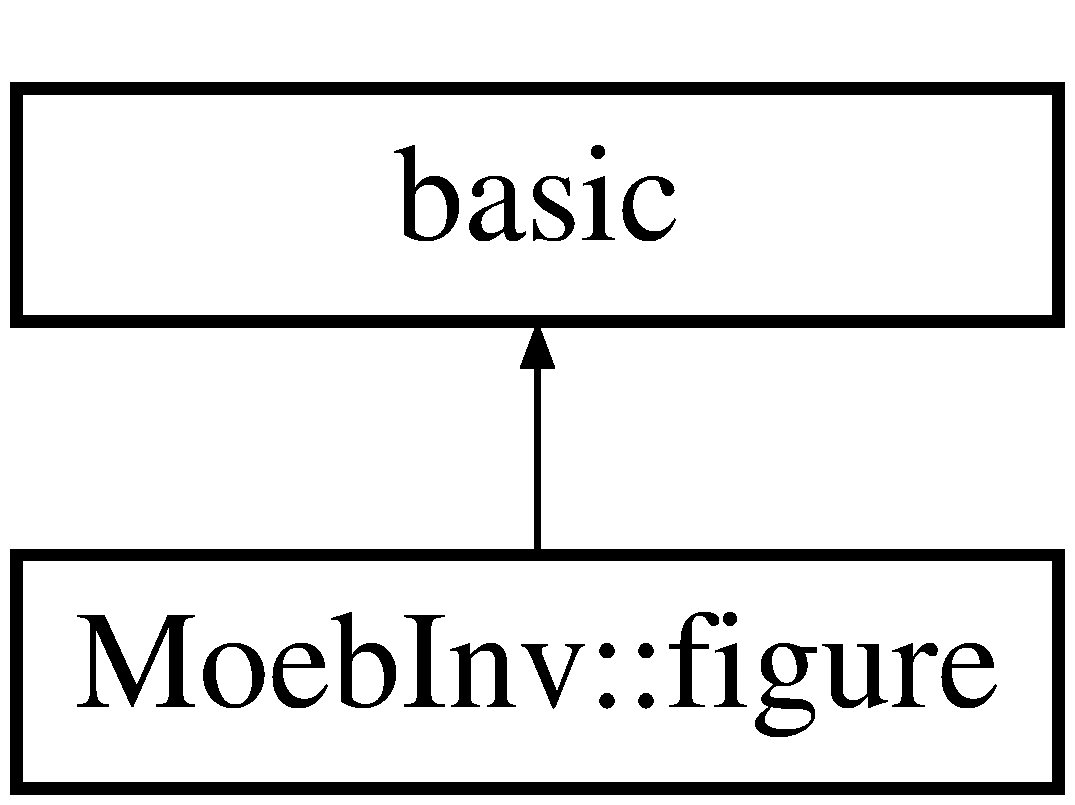
\includegraphics[height=2.000000cm]{class_moeb_inv_1_1figure}
\end{center}
\end{figure}
\subsection*{Public Member Functions}
\begin{DoxyCompactItemize}
\item 
\mbox{\Hypertarget{class_moeb_inv_1_1figure_a1344e7a1ceac3e149a541e79f36258ce}\label{class_moeb_inv_1_1figure_a1344e7a1ceac3e149a541e79f36258ce}} 
{\bfseries figure} (const ex \&Mp, const ex \&Mc=0)
\item 
\mbox{\Hypertarget{class_moeb_inv_1_1figure_ab7d6877e8dc49ee07baa3e4b433326c3}\label{class_moeb_inv_1_1figure_ab7d6877e8dc49ee07baa3e4b433326c3}} 
void {\bfseries set\+\_\+metric} (const ex \&Mp, const ex \&Mc=0)
\item 
\mbox{\Hypertarget{class_moeb_inv_1_1figure_a3a45a7757c4fa77c69e99f3855ef49a0}\label{class_moeb_inv_1_1figure_a3a45a7757c4fa77c69e99f3855ef49a0}} 
{\bfseries figure} (const ex \&Mp, const ex \&Mc, const exhashmap$<$ \mbox{\hyperlink{class_moeb_inv_1_1cycle__node}{cycle\+\_\+node}} $>$ \&N)
\item 
\mbox{\Hypertarget{class_moeb_inv_1_1figure_a27b411c4558e6e7ecc43c403da26dd82}\label{class_moeb_inv_1_1figure_a27b411c4558e6e7ecc43c403da26dd82}} 
void {\bfseries reset\+\_\+figure} ()
\item 
\mbox{\Hypertarget{class_moeb_inv_1_1figure_ac9753b10b0e1984c1b0c1e3c3c0c89aa}\label{class_moeb_inv_1_1figure_ac9753b10b0e1984c1b0c1e3c3c0c89aa}} 
ex {\bfseries add\+\_\+point} (const ex \&x, string name, string Te\+Xname=\char`\"{}\char`\"{})
\item 
\mbox{\Hypertarget{class_moeb_inv_1_1figure_acb74979c1fa2e997cb86a882233dc028}\label{class_moeb_inv_1_1figure_acb74979c1fa2e997cb86a882233dc028}} 
ex {\bfseries add\+\_\+point} (const ex \&x, const ex \&key)
\item 
\mbox{\Hypertarget{class_moeb_inv_1_1figure_aea1fd6872531d2db356e4908cb957fd5}\label{class_moeb_inv_1_1figure_aea1fd6872531d2db356e4908cb957fd5}} 
ex {\bfseries add\+\_\+cycle} (const ex \&C, string name, string Te\+Xname=\char`\"{}\char`\"{})
\item 
\mbox{\Hypertarget{class_moeb_inv_1_1figure_acfcfd11e6e2239c5a8e8821259203a77}\label{class_moeb_inv_1_1figure_acfcfd11e6e2239c5a8e8821259203a77}} 
ex {\bfseries add\+\_\+cycle} (const ex \&C, const ex \&key)
\item 
\mbox{\Hypertarget{class_moeb_inv_1_1figure_a8cbaae9347692e5d94214f3790a098e1}\label{class_moeb_inv_1_1figure_a8cbaae9347692e5d94214f3790a098e1}} 
ex {\bfseries add\+\_\+cycle\+\_\+rel} (const lst \&rel, string name, string Te\+Xname=\char`\"{}\char`\"{})
\item 
\mbox{\Hypertarget{class_moeb_inv_1_1figure_a16ef45ff448be79c670c248b8d981ea4}\label{class_moeb_inv_1_1figure_a16ef45ff448be79c670c248b8d981ea4}} 
ex {\bfseries add\+\_\+cycle\+\_\+rel} (const lst \&rel, const ex \&key)
\item 
\mbox{\Hypertarget{class_moeb_inv_1_1figure_ab0f2c91151c526ac334d3c60ceef6ce9}\label{class_moeb_inv_1_1figure_ab0f2c91151c526ac334d3c60ceef6ce9}} 
ex {\bfseries add\+\_\+cycle\+\_\+rel} (const ex \&rel, string name, string Te\+Xname=\char`\"{}\char`\"{})
\item 
\mbox{\Hypertarget{class_moeb_inv_1_1figure_a5f5ba6a6f2501cf2e9b11387e381e754}\label{class_moeb_inv_1_1figure_a5f5ba6a6f2501cf2e9b11387e381e754}} 
ex {\bfseries add\+\_\+cycle\+\_\+rel} (const ex \&rel, const ex \&key)
\item 
\mbox{\Hypertarget{class_moeb_inv_1_1figure_ae479f412608709773b1162261f441386}\label{class_moeb_inv_1_1figure_ae479f412608709773b1162261f441386}} 
ex {\bfseries add\+\_\+subfigure} (const ex \&F, const lst \&L, string name, string Te\+Xname=\char`\"{}\char`\"{})
\item 
\mbox{\Hypertarget{class_moeb_inv_1_1figure_a605a011bf174463556e9280f6ac3da65}\label{class_moeb_inv_1_1figure_a605a011bf174463556e9280f6ac3da65}} 
ex {\bfseries add\+\_\+subfigure} (const ex \&F, const lst \&L, const ex \&key)
\item 
\mbox{\Hypertarget{class_moeb_inv_1_1figure_abe4708397c90b19363fd1ec85e66b979}\label{class_moeb_inv_1_1figure_abe4708397c90b19363fd1ec85e66b979}} 
void {\bfseries move\+\_\+point} (const ex \&key, const ex \&x)
\item 
\mbox{\Hypertarget{class_moeb_inv_1_1figure_a90e556df3666a2c731c361ecdb74fe87}\label{class_moeb_inv_1_1figure_a90e556df3666a2c731c361ecdb74fe87}} 
void {\bfseries move\+\_\+cycle} (const ex \&key, const ex \&C)
\item 
\mbox{\Hypertarget{class_moeb_inv_1_1figure_ac326423d4c370fc0aa8440fa535498f4}\label{class_moeb_inv_1_1figure_ac326423d4c370fc0aa8440fa535498f4}} 
void {\bfseries remove\+\_\+cycle\+\_\+node} (const ex \&key)
\item 
\mbox{\Hypertarget{class_moeb_inv_1_1figure_a1b8387a631822fd57e4efd0735d779c8}\label{class_moeb_inv_1_1figure_a1b8387a631822fd57e4efd0735d779c8}} 
ex {\bfseries get\+\_\+cycle\+\_\+key} (string name) const
\item 
\mbox{\Hypertarget{class_moeb_inv_1_1figure_af05982b7f29f59b3e96bd0f504cecd8a}\label{class_moeb_inv_1_1figure_af05982b7f29f59b3e96bd0f504cecd8a}} 
ex {\bfseries get\+\_\+all\+\_\+keys} (const int mingen=G\+H\+O\+S\+T\+\_\+\+G\+EN+1, const int maxgen=G\+H\+O\+S\+T\+\_\+\+G\+EN) const
\item 
\mbox{\Hypertarget{class_moeb_inv_1_1figure_a2084e2b6f9cd2d72f5530d75740c19a0}\label{class_moeb_inv_1_1figure_a2084e2b6f9cd2d72f5530d75740c19a0}} 
ex {\bfseries get\+\_\+all\+\_\+keys\+\_\+sorted} (const int mingen=G\+H\+O\+S\+T\+\_\+\+G\+EN+1, const int maxgen=G\+H\+O\+S\+T\+\_\+\+G\+EN) const
\item 
\mbox{\Hypertarget{class_moeb_inv_1_1figure_ab827587a502d370aa9bbe4f6b4a39a41}\label{class_moeb_inv_1_1figure_ab827587a502d370aa9bbe4f6b4a39a41}} 
ex {\bfseries check\+\_\+rel} (const ex \&key1, const ex \&key2, P\+CR rel, bool use\+\_\+cycle\+\_\+metric=true, const ex \&parameter=0, bool corresponds=true) const
\item 
\mbox{\Hypertarget{class_moeb_inv_1_1figure_a4299a8cea895415be403a1af4235e229}\label{class_moeb_inv_1_1figure_a4299a8cea895415be403a1af4235e229}} 
ex {\bfseries measure} (const ex \&key1, const ex \&key2, P\+CR rel, bool use\+\_\+cycle\+\_\+metric=true, const ex \&parameter=0, bool corresponds=true) const
\item 
\mbox{\Hypertarget{class_moeb_inv_1_1figure_a5ade947eee85eec41f2766b794878798}\label{class_moeb_inv_1_1figure_a5ade947eee85eec41f2766b794878798}} 
ex {\bfseries get\+\_\+point\+\_\+metric} () const
\item 
\mbox{\Hypertarget{class_moeb_inv_1_1figure_abb2c58d729dcdf4beb0b25fda11cf6fe}\label{class_moeb_inv_1_1figure_abb2c58d729dcdf4beb0b25fda11cf6fe}} 
ex {\bfseries get\+\_\+cycle\+\_\+metric} () const
\item 
\mbox{\Hypertarget{class_moeb_inv_1_1figure_a1b245cd72aaf9524d34adc30b23ed76c}\label{class_moeb_inv_1_1figure_a1b245cd72aaf9524d34adc30b23ed76c}} 
ex {\bfseries get\+\_\+dim} () const
\item 
\mbox{\Hypertarget{class_moeb_inv_1_1figure_abf7111f3e5b2fe4dda176144f01147fc}\label{class_moeb_inv_1_1figure_abf7111f3e5b2fe4dda176144f01147fc}} 
ex {\bfseries get\+\_\+cycles} (const ex \&ck, bool use\+\_\+point\+\_\+metric=true) const
\item 
\mbox{\Hypertarget{class_moeb_inv_1_1figure_a3c7c1244afb27e63ec11307accad90c9}\label{class_moeb_inv_1_1figure_a3c7c1244afb27e63ec11307accad90c9}} 
ex {\bfseries get\+\_\+cycles} (const ex \&ck, const ex \&metric) const
\item 
\mbox{\Hypertarget{class_moeb_inv_1_1figure_a17c3d1598318d1eacfbd2e7380b970d0}\label{class_moeb_inv_1_1figure_a17c3d1598318d1eacfbd2e7380b970d0}} 
ex {\bfseries get\+\_\+generation} (const ex \&ck) const
\item 
\mbox{\Hypertarget{class_moeb_inv_1_1figure_af47df5474587449058e599dd89fab073}\label{class_moeb_inv_1_1figure_af47df5474587449058e599dd89fab073}} 
ex {\bfseries apply} (P\+E\+V\+AL func, bool use\+\_\+cycle\+\_\+metric=true, const ex \&param=0) const
\item 
\mbox{\Hypertarget{class_moeb_inv_1_1figure_a49cd358c9efc24bdfdf07388e71959ad}\label{class_moeb_inv_1_1figure_a49cd358c9efc24bdfdf07388e71959ad}} 
void {\bfseries asy\+\_\+draw} (ostream \&ost=std\+::cout, ostream \&err=std\+::cerr, const string picture=\char`\"{}\char`\"{}, const ex \&xmin=-\/5, const ex \&xmax=5, const ex \&ymin=-\/5, const ex \&ymax=5, asy\+\_\+style style=default\+\_\+asy, label\+\_\+string lstring=default\+\_\+label, bool with\+\_\+realline=true, bool with\+\_\+header=true, int points\+\_\+per\+\_\+arc=0, const string imaginary\+\_\+options=\char`\"{}rgb(0,.\+9,0)+4pt\char`\"{}, bool with\+\_\+labels=true) const
\item 
\mbox{\Hypertarget{class_moeb_inv_1_1figure_a6fcc62ff2ef2b854c45cebfe466dd883}\label{class_moeb_inv_1_1figure_a6fcc62ff2ef2b854c45cebfe466dd883}} 
void {\bfseries asy\+\_\+write} (int size=300, const ex \&xmin=-\/5, const ex \&xmax=5, const ex \&ymin=-\/5, const ex \&ymax=5, string name=\char`\"{}figure-\/\mbox{\hyperlink{classview}{view}}-\/tmp\char`\"{}, string format=\char`\"{}\char`\"{}, asy\+\_\+style style=default\+\_\+asy, label\+\_\+string lstring=default\+\_\+label, bool with\+\_\+realline=true, bool with\+\_\+header=true, int points\+\_\+per\+\_\+arc=0, const string imaginary\+\_\+options=\char`\"{}rgb(0,.\+9,0)+4pt\char`\"{}, bool rm\+\_\+asy\+\_\+file=true, bool with\+\_\+labels=true) const
\item 
\mbox{\Hypertarget{class_moeb_inv_1_1figure_a95db99defd205929ff60c4d235c44ef2}\label{class_moeb_inv_1_1figure_a95db99defd205929ff60c4d235c44ef2}} 
void {\bfseries asy\+\_\+animate} (const ex \&val, int size=300, const ex \&xmin=-\/5, const ex \&xmax=5, const ex \&ymin=-\/5, const ex \&ymax=5, string name=\char`\"{}figure-\/animatecf-\/tmp\char`\"{}, string format=\char`\"{}pdf\char`\"{}, asy\+\_\+style style=default\+\_\+asy, label\+\_\+string lstring=default\+\_\+label, bool with\+\_\+realline=true, bool with\+\_\+header=true, int points\+\_\+per\+\_\+arc=0, const string imaginary\+\_\+options=\char`\"{}rgb(0,.\+9,0)+4pt\char`\"{}, const string values\+\_\+position=\char`\"{}bl\char`\"{}, bool rm\+\_\+asy\+\_\+file=true, bool with\+\_\+labels=true) const
\item 
\mbox{\Hypertarget{class_moeb_inv_1_1figure_a02bf77ec6aad9df7729cb0cbcd13cc86}\label{class_moeb_inv_1_1figure_a02bf77ec6aad9df7729cb0cbcd13cc86}} 
\mbox{\hyperlink{class_moeb_inv_1_1figure}{figure}} {\bfseries freeze} () const
\item 
\mbox{\Hypertarget{class_moeb_inv_1_1figure_a710ef7010d067dbb9236982721f77aa3}\label{class_moeb_inv_1_1figure_a710ef7010d067dbb9236982721f77aa3}} 
\mbox{\hyperlink{class_moeb_inv_1_1figure}{figure}} {\bfseries unfreeze} () const
\item 
\mbox{\Hypertarget{class_moeb_inv_1_1figure_acb91de7431b221e254dc346d674bf8ee}\label{class_moeb_inv_1_1figure_acb91de7431b221e254dc346d674bf8ee}} 
\mbox{\hyperlink{class_moeb_inv_1_1figure}{figure}} {\bfseries set\+\_\+float\+\_\+eval} ()
\item 
\mbox{\Hypertarget{class_moeb_inv_1_1figure_abbabd3387426db22e8b91ada8aee1f5f}\label{class_moeb_inv_1_1figure_abbabd3387426db22e8b91ada8aee1f5f}} 
\mbox{\hyperlink{class_moeb_inv_1_1figure}{figure}} {\bfseries set\+\_\+exact\+\_\+eval} ()
\item 
\mbox{\Hypertarget{class_moeb_inv_1_1figure_a0d9d0212994fd3003ba7f770fd0971e3}\label{class_moeb_inv_1_1figure_a0d9d0212994fd3003ba7f770fd0971e3}} 
void {\bfseries set\+\_\+asy\+\_\+style} (const ex \&key, string opt)
\item 
\mbox{\Hypertarget{class_moeb_inv_1_1figure_ac59852184f352895f3398f6c82fdc799}\label{class_moeb_inv_1_1figure_ac59852184f352895f3398f6c82fdc799}} 
string {\bfseries get\+\_\+asy\+\_\+style} (const ex \&key) const
\item 
\mbox{\Hypertarget{class_moeb_inv_1_1figure_aedaad1298de3ef67d89f1526df799b2c}\label{class_moeb_inv_1_1figure_aedaad1298de3ef67d89f1526df799b2c}} 
void {\bfseries arrangement\+\_\+write} (string name, int first\+\_\+gen=0) const
\item 
\mbox{\Hypertarget{class_moeb_inv_1_1figure_afabc986665580bfeefee5cffca95a6c3}\label{class_moeb_inv_1_1figure_afabc986665580bfeefee5cffca95a6c3}} 
void {\bfseries save} (const char $\ast$file\+\_\+name, const char $\ast$fig\+\_\+name=\char`\"{}myfig\char`\"{}) const
\item 
\mbox{\Hypertarget{class_moeb_inv_1_1figure_ae920a70e851e5d384334717dda4a2c9f}\label{class_moeb_inv_1_1figure_ae920a70e851e5d384334717dda4a2c9f}} 
{\bfseries figure} (const char $\ast$file\+\_\+name, string fig\+\_\+name=\char`\"{}myfig\char`\"{})
\item 
\mbox{\Hypertarget{class_moeb_inv_1_1figure_a32747e3cf3b9924e3d5cd26581d06eb7}\label{class_moeb_inv_1_1figure_a32747e3cf3b9924e3d5cd26581d06eb7}} 
void {\bfseries info\+\_\+write} (string whole\+\_\+text)
\item 
\mbox{\Hypertarget{class_moeb_inv_1_1figure_a7c189df048d3428e392941c44cf836c0}\label{class_moeb_inv_1_1figure_a7c189df048d3428e392941c44cf836c0}} 
void {\bfseries info\+\_\+append} (string more\+\_\+text)
\item 
\mbox{\Hypertarget{class_moeb_inv_1_1figure_ac6984f346a1a9244d137275cde32ccc2}\label{class_moeb_inv_1_1figure_ac6984f346a1a9244d137275cde32ccc2}} 
string {\bfseries info\+\_\+read} () const
\item 
\mbox{\Hypertarget{class_moeb_inv_1_1figure_a6271596d854119c11008b9d083c2d169}\label{class_moeb_inv_1_1figure_a6271596d854119c11008b9d083c2d169}} 
exhashmap$<$ \mbox{\hyperlink{class_moeb_inv_1_1cycle__node}{cycle\+\_\+node}} $>$ {\bfseries get\+\_\+nodes} () const
\item 
\mbox{\Hypertarget{class_moeb_inv_1_1figure_a10f4beaf7cf4322b2b6c6a155e2e4ca2}\label{class_moeb_inv_1_1figure_a10f4beaf7cf4322b2b6c6a155e2e4ca2}} 
ex {\bfseries get\+\_\+real\+\_\+line} () const
\item 
\mbox{\Hypertarget{class_moeb_inv_1_1figure_a70c256f1a0b7e27d6e6f6f369108ff01}\label{class_moeb_inv_1_1figure_a70c256f1a0b7e27d6e6f6f369108ff01}} 
ex {\bfseries get\+\_\+infinity} () const
\item 
\mbox{\Hypertarget{class_moeb_inv_1_1figure_a96c851ea4f8878c4416bdbeb7ace896b}\label{class_moeb_inv_1_1figure_a96c851ea4f8878c4416bdbeb7ace896b}} 
int {\bfseries get\+\_\+max\+\_\+generation} () const
\item 
\mbox{\Hypertarget{class_moeb_inv_1_1figure_a7f0306adf95eeb332f67060e3bcad6df}\label{class_moeb_inv_1_1figure_a7f0306adf95eeb332f67060e3bcad6df}} 
size\+\_\+t {\bfseries nops} () const
\item 
\mbox{\Hypertarget{class_moeb_inv_1_1figure_afa4b697cf4a3807f2841f6499421833f}\label{class_moeb_inv_1_1figure_afa4b697cf4a3807f2841f6499421833f}} 
ex {\bfseries op} (size\+\_\+t i) const
\item 
\mbox{\Hypertarget{class_moeb_inv_1_1figure_a3f5bc6243d635a5f7c1b0e4a659f05e6}\label{class_moeb_inv_1_1figure_a3f5bc6243d635a5f7c1b0e4a659f05e6}} 
ex {\bfseries evalf} (int level=0) const
\item 
\mbox{\Hypertarget{class_moeb_inv_1_1figure_ab8fc6b722bb0f9f3472106b64d10c7bc}\label{class_moeb_inv_1_1figure_ab8fc6b722bb0f9f3472106b64d10c7bc}} 
\mbox{\hyperlink{class_moeb_inv_1_1figure}{figure}} {\bfseries subs} (const ex \&e, unsigned options=0) const
\item 
\mbox{\Hypertarget{class_moeb_inv_1_1figure_ac2b38f061d3125b11adda821698b95dd}\label{class_moeb_inv_1_1figure_ac2b38f061d3125b11adda821698b95dd}} 
ex {\bfseries subs} (const exmap \&m, unsigned options=0) const
\item 
\mbox{\Hypertarget{class_moeb_inv_1_1figure_a947540d1cdd36573716aaad9755cb14a}\label{class_moeb_inv_1_1figure_a947540d1cdd36573716aaad9755cb14a}} 
void {\bfseries archive} (archive\+\_\+node \&n) const
\item 
\mbox{\Hypertarget{class_moeb_inv_1_1figure_a6550d2bbdf8b71b942a7f2b38e16ee7b}\label{class_moeb_inv_1_1figure_a6550d2bbdf8b71b942a7f2b38e16ee7b}} 
void {\bfseries read\+\_\+archive} (const archive\+\_\+node \&n, lst \&sym\+\_\+lst)
\item 
\mbox{\Hypertarget{class_moeb_inv_1_1figure_a5821cfff25a0f64069a9ade4ed2e0836}\label{class_moeb_inv_1_1figure_a5821cfff25a0f64069a9ade4ed2e0836}} 
bool {\bfseries info} (unsigned inf) const
\item 
\mbox{\Hypertarget{class_moeb_inv_1_1figure_a556b55595bd5737909946e2f98b3e081}\label{class_moeb_inv_1_1figure_a556b55595bd5737909946e2f98b3e081}} 
ex {\bfseries get\+\_\+cycle\+\_\+node} (const ex \&ck) const
\item 
\mbox{\Hypertarget{class_moeb_inv_1_1figure_a8a759812f57a57d752edb9b5b96a97ce}\label{class_moeb_inv_1_1figure_a8a759812f57a57d752edb9b5b96a97ce}} 
void {\bfseries do\+\_\+print\+\_\+double} (const print\+\_\+dflt \&con, unsigned level) const
\end{DoxyCompactItemize}
\subsection*{Protected Member Functions}
\begin{DoxyCompactItemize}
\item 
\mbox{\Hypertarget{class_moeb_inv_1_1figure_a53d5e42db02edb8cd83fcfd007721e82}\label{class_moeb_inv_1_1figure_a53d5e42db02edb8cd83fcfd007721e82}} 
ex {\bfseries update\+\_\+cycle\+\_\+node} (const ex \&key, const lst \&eq\+\_\+cond=lst\{\}, const lst \&neq\+\_\+cond=lst\{\}, lst res=lst\{\}, size\+\_\+t level=0)
\item 
\mbox{\Hypertarget{class_moeb_inv_1_1figure_a344c3bd7f96835710033f93537810599}\label{class_moeb_inv_1_1figure_a344c3bd7f96835710033f93537810599}} 
void {\bfseries set\+\_\+cycle} (const ex \&key, const ex \&C)
\item 
\mbox{\Hypertarget{class_moeb_inv_1_1figure_acf7b35e710a1c3436bb8a9177c6c1506}\label{class_moeb_inv_1_1figure_acf7b35e710a1c3436bb8a9177c6c1506}} 
ex {\bfseries evaluate\+\_\+cycle} (const ex \&symbolic, const lst \&cond) const
\item 
\mbox{\Hypertarget{class_moeb_inv_1_1figure_ad040638cbdce1a8b2ccea5651cad3c5c}\label{class_moeb_inv_1_1figure_ad040638cbdce1a8b2ccea5651cad3c5c}} 
void {\bfseries do\+\_\+print} (const print\+\_\+dflt \&con, unsigned level) const
\item 
\mbox{\Hypertarget{class_moeb_inv_1_1figure_a8c2652c1778c7f22416916d11d5540f9}\label{class_moeb_inv_1_1figure_a8c2652c1778c7f22416916d11d5540f9}} 
return\+\_\+type\+\_\+t {\bfseries return\+\_\+type\+\_\+tinfo} () const
\item 
\mbox{\Hypertarget{class_moeb_inv_1_1figure_a27a6f97a9955992111d7c2ce7c099ff2}\label{class_moeb_inv_1_1figure_a27a6f97a9955992111d7c2ce7c099ff2}} 
void {\bfseries update\+\_\+node\+\_\+lst} (const ex \&inlist)
\item 
\mbox{\Hypertarget{class_moeb_inv_1_1figure_a676003f88f8aac028bb98d4e8ccebcc3}\label{class_moeb_inv_1_1figure_a676003f88f8aac028bb98d4e8ccebcc3}} 
\mbox{\hyperlink{class_moeb_inv_1_1figure}{figure}} {\bfseries update\+\_\+cycles} ()
\end{DoxyCompactItemize}
\subsection*{Protected Attributes}
\begin{DoxyCompactItemize}
\item 
\mbox{\Hypertarget{class_moeb_inv_1_1figure_aba3eaece2e5221edca5631b1a24e3bb1}\label{class_moeb_inv_1_1figure_aba3eaece2e5221edca5631b1a24e3bb1}} 
ex {\bfseries real\+\_\+line}
\item 
\mbox{\Hypertarget{class_moeb_inv_1_1figure_a2bac895d87f790c9a2e137bba1a8b234}\label{class_moeb_inv_1_1figure_a2bac895d87f790c9a2e137bba1a8b234}} 
ex {\bfseries infinity}
\item 
\mbox{\Hypertarget{class_moeb_inv_1_1figure_acf90b212a1c28c2982759754d75b5b5f}\label{class_moeb_inv_1_1figure_acf90b212a1c28c2982759754d75b5b5f}} 
ex {\bfseries point\+\_\+metric}
\item 
\mbox{\Hypertarget{class_moeb_inv_1_1figure_a3c3815eb39030137dbedcbd43d66cef5}\label{class_moeb_inv_1_1figure_a3c3815eb39030137dbedcbd43d66cef5}} 
ex {\bfseries cycle\+\_\+metric}
\item 
\mbox{\Hypertarget{class_moeb_inv_1_1figure_a97a66de49a1b3480321660f4b53e0962}\label{class_moeb_inv_1_1figure_a97a66de49a1b3480321660f4b53e0962}} 
exhashmap$<$ \mbox{\hyperlink{class_moeb_inv_1_1cycle__node}{cycle\+\_\+node}} $>$ {\bfseries nodes}
\item 
\mbox{\Hypertarget{class_moeb_inv_1_1figure_a004e8547d3d8cd091d7220c2641fa684}\label{class_moeb_inv_1_1figure_a004e8547d3d8cd091d7220c2641fa684}} 
bool {\bfseries float\+\_\+evaluation} =false
\item 
\mbox{\Hypertarget{class_moeb_inv_1_1figure_a8f9ef2655ffa1e826426d0b29450da5c}\label{class_moeb_inv_1_1figure_a8f9ef2655ffa1e826426d0b29450da5c}} 
string {\bfseries info\+\_\+text}
\item 
\mbox{\Hypertarget{class_moeb_inv_1_1figure_a069a8553a3d439c4b2a35a23b55c6ab0}\label{class_moeb_inv_1_1figure_a069a8553a3d439c4b2a35a23b55c6ab0}} 
ex {\bfseries k}
\item 
\mbox{\Hypertarget{class_moeb_inv_1_1figure_a23cad935b5579c07b151efce7598a760}\label{class_moeb_inv_1_1figure_a23cad935b5579c07b151efce7598a760}} 
ex {\bfseries m}
\item 
\mbox{\Hypertarget{class_moeb_inv_1_1figure_a41a8b6bdba7df3ad2a7ebd70202953b6}\label{class_moeb_inv_1_1figure_a41a8b6bdba7df3ad2a7ebd70202953b6}} 
lst {\bfseries l}
\end{DoxyCompactItemize}


The documentation for this class was generated from the following file\+:\begin{DoxyCompactItemize}
\item 
/\+Users/lukehutton/\+One\+Drive -\/ University of Leeds/\+University/\+Computer Science/\+Internship/moebinv-\/gui/lib/moebinv-\/3.\+2/include/figure.\+h\end{DoxyCompactItemize}

\hypertarget{classfigure_undo_command}{}\section{figure\+Undo\+Command Class Reference}
\label{classfigure_undo_command}\index{figure\+Undo\+Command@{figure\+Undo\+Command}}
Inheritance diagram for figure\+Undo\+Command\+:\begin{figure}[H]
\begin{center}
\leavevmode
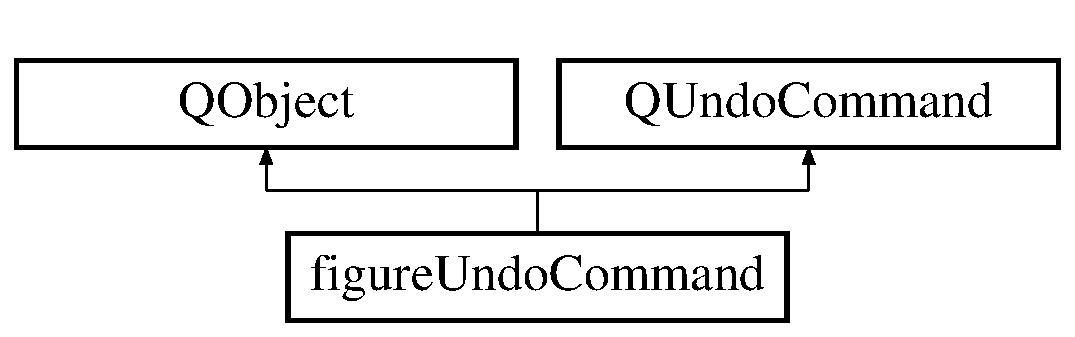
\includegraphics[height=2.000000cm]{classfigure_undo_command}
\end{center}
\end{figure}
\subsection*{Signals}
\begin{DoxyCompactItemize}
\item 
\mbox{\Hypertarget{classfigure_undo_command_a0826ae627f25daaa23ba9ccdd7e8fda2}\label{classfigure_undo_command_a0826ae627f25daaa23ba9ccdd7e8fda2}} 
void {\bfseries scene\+Invalid} (const \mbox{\hyperlink{class_moeb_inv_1_1figure}{Moeb\+Inv\+::figure}} \&replacement\+Figure)
\end{DoxyCompactItemize}
\subsection*{Public Member Functions}
\begin{DoxyCompactItemize}
\item 
\mbox{\hyperlink{classfigure_undo_command_af29d6f2ed7bcff9fdae44a83707d0d76}{figure\+Undo\+Command}} (\mbox{\hyperlink{class_moeb_inv_1_1figure}{Moeb\+Inv\+::figure}} original\+Figure, \mbox{\hyperlink{class_moeb_inv_1_1figure}{Moeb\+Inv\+::figure}} changed\+Figure, Q\+Undo\+Command $\ast$parent=nullptr)
\begin{DoxyCompactList}\small\item\em \mbox{\hyperlink{classfigure_undo_command_af29d6f2ed7bcff9fdae44a83707d0d76}{figure\+Undo\+Command\+::figure\+Undo\+Command}} \end{DoxyCompactList}\item 
void \mbox{\hyperlink{classfigure_undo_command_a9e733f81f847b07673f141bf13c5aace}{undo}} ()
\begin{DoxyCompactList}\small\item\em \mbox{\hyperlink{classfigure_undo_command_a9e733f81f847b07673f141bf13c5aace}{figure\+Undo\+Command\+::undo}} \end{DoxyCompactList}\item 
void \mbox{\hyperlink{classfigure_undo_command_aec81e1bda86663871b7ff1cb6e8d5fda}{redo}} ()
\begin{DoxyCompactList}\small\item\em \mbox{\hyperlink{classfigure_undo_command_aec81e1bda86663871b7ff1cb6e8d5fda}{figure\+Undo\+Command\+::redo}} \end{DoxyCompactList}\item 
\mbox{\Hypertarget{classfigure_undo_command_a571773dcb5236289e16f0d444e9785e5}\label{classfigure_undo_command_a571773dcb5236289e16f0d444e9785e5}} 
Q\+String {\bfseries node\+\_\+label} (Gi\+Na\+C\+::ex name)
\end{DoxyCompactItemize}


\subsection{Constructor \& Destructor Documentation}
\mbox{\Hypertarget{classfigure_undo_command_af29d6f2ed7bcff9fdae44a83707d0d76}\label{classfigure_undo_command_af29d6f2ed7bcff9fdae44a83707d0d76}} 
\index{figure\+Undo\+Command@{figure\+Undo\+Command}!figure\+Undo\+Command@{figure\+Undo\+Command}}
\index{figure\+Undo\+Command@{figure\+Undo\+Command}!figure\+Undo\+Command@{figure\+Undo\+Command}}
\subsubsection{\texorpdfstring{figure\+Undo\+Command()}{figureUndoCommand()}}
{\footnotesize\ttfamily figure\+Undo\+Command\+::figure\+Undo\+Command (\begin{DoxyParamCaption}\item[{\mbox{\hyperlink{class_moeb_inv_1_1figure}{Moeb\+Inv\+::figure}}}]{original\+Figure,  }\item[{\mbox{\hyperlink{class_moeb_inv_1_1figure}{Moeb\+Inv\+::figure}}}]{changed\+Figure,  }\item[{Q\+Undo\+Command $\ast$}]{parent = {\ttfamily nullptr} }\end{DoxyParamCaption})}



\mbox{\hyperlink{classfigure_undo_command_af29d6f2ed7bcff9fdae44a83707d0d76}{figure\+Undo\+Command\+::figure\+Undo\+Command}} 


\begin{DoxyParams}{Parameters}
{\em original\+Figure} & \\
\hline
{\em changed\+Figure} & \\
\hline
{\em parent} & Figure undo command constructor. This object is inherited from Q\+Undo\+Command and allows any changes made to a figure to be stored in the undo stack. \\
\hline
\end{DoxyParams}


\subsection{Member Function Documentation}
\mbox{\Hypertarget{classfigure_undo_command_aec81e1bda86663871b7ff1cb6e8d5fda}\label{classfigure_undo_command_aec81e1bda86663871b7ff1cb6e8d5fda}} 
\index{figure\+Undo\+Command@{figure\+Undo\+Command}!redo@{redo}}
\index{redo@{redo}!figure\+Undo\+Command@{figure\+Undo\+Command}}
\subsubsection{\texorpdfstring{redo()}{redo()}}
{\footnotesize\ttfamily void figure\+Undo\+Command\+::redo (\begin{DoxyParamCaption}{ }\end{DoxyParamCaption})}



\mbox{\hyperlink{classfigure_undo_command_aec81e1bda86663871b7ff1cb6e8d5fda}{figure\+Undo\+Command\+::redo}} 

Redo an action and resore the figure after it has been changed. \mbox{\Hypertarget{classfigure_undo_command_a9e733f81f847b07673f141bf13c5aace}\label{classfigure_undo_command_a9e733f81f847b07673f141bf13c5aace}} 
\index{figure\+Undo\+Command@{figure\+Undo\+Command}!undo@{undo}}
\index{undo@{undo}!figure\+Undo\+Command@{figure\+Undo\+Command}}
\subsubsection{\texorpdfstring{undo()}{undo()}}
{\footnotesize\ttfamily void figure\+Undo\+Command\+::undo (\begin{DoxyParamCaption}{ }\end{DoxyParamCaption})}



\mbox{\hyperlink{classfigure_undo_command_a9e733f81f847b07673f141bf13c5aace}{figure\+Undo\+Command\+::undo}} 

Undo an action and resore the previous figure before the change. 

The documentation for this class was generated from the following files\+:\begin{DoxyCompactItemize}
\item 
/\+Users/lukehutton/\+One\+Drive -\/ University of Leeds/\+University/\+Computer Science/\+Internship/moebinv-\/gui/include/figureundocommand.\+h\item 
/\+Users/lukehutton/\+One\+Drive -\/ University of Leeds/\+University/\+Computer Science/\+Internship/moebinv-\/gui/moebinv-\/gui-\/build/moc\+\_\+figureundocommand.\+cpp\item 
/\+Users/lukehutton/\+One\+Drive -\/ University of Leeds/\+University/\+Computer Science/\+Internship/moebinv-\/gui/src/figureundocommand.\+cpp\end{DoxyCompactItemize}

\hypertarget{structgen_key}{}\section{gen\+Key Struct Reference}
\label{structgen_key}\index{gen\+Key@{gen\+Key}}


{\ttfamily \#include $<$vis.\+h$>$}

\subsection*{Public Attributes}
\begin{DoxyCompactItemize}
\item 
int \mbox{\hyperlink{structgen_key_ae5256faedda05a8b25b760c8bdeb75c4}{gen}}
\item 
string \mbox{\hyperlink{structgen_key_a76a2731affcdaf847724d065a9140000}{key}}
\end{DoxyCompactItemize}


\subsection{Detailed Description}
structure to store generation and key data of objects. 

\subsection{Member Data Documentation}
\mbox{\Hypertarget{structgen_key_ae5256faedda05a8b25b760c8bdeb75c4}\label{structgen_key_ae5256faedda05a8b25b760c8bdeb75c4}} 
\index{gen\+Key@{gen\+Key}!gen@{gen}}
\index{gen@{gen}!gen\+Key@{gen\+Key}}
\subsubsection{\texorpdfstring{gen}{gen}}
{\footnotesize\ttfamily int gen\+Key\+::gen}

positive integer for object\textquotesingle{}s generation. \mbox{\Hypertarget{structgen_key_a76a2731affcdaf847724d065a9140000}\label{structgen_key_a76a2731affcdaf847724d065a9140000}} 
\index{gen\+Key@{gen\+Key}!key@{key}}
\index{key@{key}!gen\+Key@{gen\+Key}}
\subsubsection{\texorpdfstring{key}{key}}
{\footnotesize\ttfamily string gen\+Key\+::key}

object\textquotesingle{}s key value. 

The documentation for this struct was generated from the following file\+:\begin{DoxyCompactItemize}
\item 
/\+Users/lukehutton/\+One\+Drive -\/ University of Leeds/\+University/\+Computer Science/\+Internship/moebinv-\/gui/lib/moebinv-\/3.\+2/cycle3\+D-\/visualiser/vis.\+h\end{DoxyCompactItemize}

\hypertarget{classgraphic_cycle}{}\section{graphic\+Cycle Class Reference}
\label{classgraphic_cycle}\index{graphic\+Cycle@{graphic\+Cycle}}


The \mbox{\hyperlink{classgraphic_cycle}{graphic\+Cycle}} class.  




{\ttfamily \#include $<$graphiccycle.\+h$>$}

Inheritance diagram for graphic\+Cycle\+:\begin{figure}[H]
\begin{center}
\leavevmode
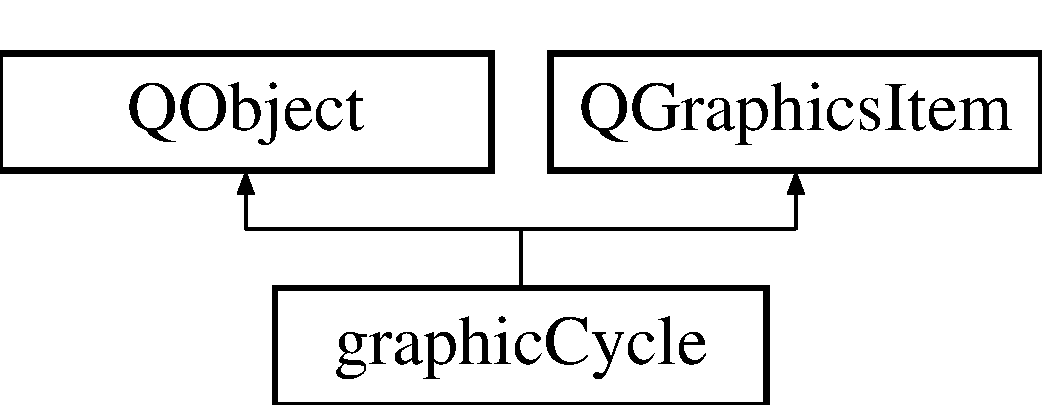
\includegraphics[height=2.000000cm]{classgraphic_cycle}
\end{center}
\end{figure}
\subsection*{Public Slots}
\begin{DoxyCompactItemize}
\item 
void \mbox{\hyperlink{classgraphic_cycle_a54708026fc7ea647f431263990872cdf}{set\+Hover}} ()
\begin{DoxyCompactList}\small\item\em \mbox{\hyperlink{classgraphic_cycle_a54708026fc7ea647f431263990872cdf}{graphic\+Cycle\+::set\+Hover}} set the hover style of the object. \end{DoxyCompactList}\item 
void \mbox{\hyperlink{classgraphic_cycle_a7d9d805ccc83dcf16623c969ad48b6a5}{unset\+Hover}} ()
\begin{DoxyCompactList}\small\item\em \mbox{\hyperlink{classgraphic_cycle_a7d9d805ccc83dcf16623c969ad48b6a5}{graphic\+Cycle\+::unset\+Hover}} unset the object hover \end{DoxyCompactList}\item 
void \mbox{\hyperlink{classgraphic_cycle_a48965c220e8fad0181f1f793c17fb73c}{set\+Colour}} (Q\+Color colour)
\begin{DoxyCompactList}\small\item\em \mbox{\hyperlink{classgraphic_cycle_a48965c220e8fad0181f1f793c17fb73c}{graphic\+Cycle\+::set\+Colour}} set the colour of the graphic cycle. \end{DoxyCompactList}\item 
void \mbox{\hyperlink{classgraphic_cycle_aa02ce6a22ddb0ae859ab6dac49a0570a}{set\+Line\+Width}} (double weight)
\begin{DoxyCompactList}\small\item\em \mbox{\hyperlink{classgraphic_cycle_aa02ce6a22ddb0ae859ab6dac49a0570a}{graphic\+Cycle\+::set\+Line\+Width}} set the weight of the graphic cycle. \end{DoxyCompactList}\item 
void \mbox{\hyperlink{classgraphic_cycle_a96f1a1d6c958bfba3789a13c156f9795}{set\+Line\+Style}} (int style)
\begin{DoxyCompactList}\small\item\em \mbox{\hyperlink{classgraphic_cycle_a96f1a1d6c958bfba3789a13c156f9795}{graphic\+Cycle\+::set\+Line\+Style}} set the style of the graphic cycle. \end{DoxyCompactList}\item 
void \mbox{\hyperlink{classgraphic_cycle_a173e5e3dfb0dde41c8046a53086e02ab}{mouse\+Stopped}} ()
\begin{DoxyCompactList}\small\item\em \mbox{\hyperlink{classgraphic_cycle_a173e5e3dfb0dde41c8046a53086e02ab}{graphic\+Cycle\+::mouse\+Stopped}} \end{DoxyCompactList}\item 
void \mbox{\hyperlink{classgraphic_cycle_af79bfc4ed813bab595a2a721475a7199}{cancel\+Movement}} ()
\begin{DoxyCompactList}\small\item\em \mbox{\hyperlink{classgraphic_cycle_af79bfc4ed813bab595a2a721475a7199}{graphic\+Cycle\+::cancel\+Movement}} \end{DoxyCompactList}\end{DoxyCompactItemize}
\subsection*{Signals}
\begin{DoxyCompactItemize}
\item 
\mbox{\Hypertarget{classgraphic_cycle_ae60f6c55734308b7811d0f5ff9116227}\label{classgraphic_cycle_ae60f6c55734308b7811d0f5ff9116227}} 
void {\bfseries find\+Cycle\+In\+Tree} (Gi\+Na\+C\+::ex cycle)
\item 
\mbox{\Hypertarget{classgraphic_cycle_aa36164d21bdd1b7cde5b26407f330d49}\label{classgraphic_cycle_aa36164d21bdd1b7cde5b26407f330d49}} 
void {\bfseries scene\+Invalid} ()
\item 
\mbox{\Hypertarget{classgraphic_cycle_a04f2deb84f4a748e8bb9dba7a43eb653}\label{classgraphic_cycle_a04f2deb84f4a748e8bb9dba7a43eb653}} 
void {\bfseries changes\+Made\+To\+Figure} (const Moeb\+Inv\+::figure \&original\+Figure, const Moeb\+Inv\+::figure \&changed\+Figure)
\end{DoxyCompactItemize}
\subsection*{Public Member Functions}
\begin{DoxyCompactItemize}
\item 
\mbox{\hyperlink{classgraphic_cycle_a89c2914fab32a0e10b2d53491535c173}{graphic\+Cycle}} (Moeb\+Inv\+::figure $\ast$f, Gi\+Na\+C\+::ex c, double $\ast$relative\+Scale\+Factor, \mbox{\hyperlink{classcycle_context_menu}{cycle\+Context\+Menu}} $\ast$menu, struct \mbox{\hyperlink{structcycle_style_data}{cycle\+Style\+Data}} style\+Data)
\begin{DoxyCompactList}\small\item\em \mbox{\hyperlink{classgraphic_cycle_a89c2914fab32a0e10b2d53491535c173}{graphic\+Cycle\+::graphic\+Cycle}} graphicd cycle constructor. \end{DoxyCompactList}\item 
Q\+String \mbox{\hyperlink{classgraphic_cycle_ae55bb7487a8baac738b88e8c1bd0515e}{get\+Cycle\+Label}} ()
\begin{DoxyCompactList}\small\item\em \mbox{\hyperlink{classgraphic_cycle_ae55bb7487a8baac738b88e8c1bd0515e}{graphic\+Cycle\+::get\+Cycle\+Label}} get the cycle label. \end{DoxyCompactList}\item 
double $\ast$ \mbox{\hyperlink{classgraphic_cycle_a80b533c2477a08f98506202d94bad7bc}{get\+Relative\+Scale\+Factor}} ()
\begin{DoxyCompactList}\small\item\em \mbox{\hyperlink{classgraphic_cycle_a80b533c2477a08f98506202d94bad7bc}{graphic\+Cycle\+::get\+Relative\+Scale\+Factor}} get the scale factor of the scene. \end{DoxyCompactList}\item 
\mbox{\hyperlink{classcycle_context_menu}{cycle\+Context\+Menu}} $\ast$ \mbox{\hyperlink{classgraphic_cycle_a4e090d82ba2e37bee415c95630abe061}{get\+Context\+Menu}} ()
\begin{DoxyCompactList}\small\item\em \mbox{\hyperlink{classgraphic_cycle_a4e090d82ba2e37bee415c95630abe061}{graphic\+Cycle\+::get\+Context\+Menu}} get the context menu linked to the scene. \end{DoxyCompactList}\item 
\mbox{\Hypertarget{classgraphic_cycle_a10e61352945ca9b32b83e528e2fc6853}\label{classgraphic_cycle_a10e61352945ca9b32b83e528e2fc6853}} 
bool \mbox{\hyperlink{classgraphic_cycle_a10e61352945ca9b32b83e528e2fc6853}{get\+Item\+Is\+Grabbed}} ()
\begin{DoxyCompactList}\small\item\em \mbox{\hyperlink{classgraphic_cycle_a10e61352945ca9b32b83e528e2fc6853}{graphic\+Cycle\+::get\+Item\+Is\+Grabbed}} get whether the item is being moved. \end{DoxyCompactList}\item 
void \mbox{\hyperlink{classgraphic_cycle_a44dc93e5f66707fd102c2acccbef076c}{add\+Child}} (int child\+Type, const double \&x, const double \&y, const double \&c=0, const double \&radius=0)
\begin{DoxyCompactList}\small\item\em \mbox{\hyperlink{classgraphic_cycle_a44dc93e5f66707fd102c2acccbef076c}{graphic\+Cycle\+::add\+Child}} Add a new child to graphic cycle. \end{DoxyCompactList}\item 
virtual void \mbox{\hyperlink{classgraphic_cycle_a746393c5d92838147094dadee5c289f5}{paint}} (Q\+Painter $\ast$painter, const Q\+Style\+Option\+Graphics\+Item $\ast$option, Q\+Widget $\ast$widget)
\begin{DoxyCompactList}\small\item\em \mbox{\hyperlink{classgraphic_cycle_a746393c5d92838147094dadee5c289f5}{graphic\+Cycle\+::paint}} Paint the object to the scene. \end{DoxyCompactList}\item 
virtual Q\+RectF \mbox{\hyperlink{classgraphic_cycle_a4db310e0fdbccffefc7404c47eb73607}{bounding\+Rect}} () const
\begin{DoxyCompactList}\small\item\em \mbox{\hyperlink{classgraphic_cycle_a4db310e0fdbccffefc7404c47eb73607}{graphic\+Cycle\+::bounding\+Rect}} Define the bounding rect. \end{DoxyCompactList}\item 
void \mbox{\hyperlink{classgraphic_cycle_af731c349d665b784291187ad4b0a71d9}{mouse\+Press\+Event}} (Q\+Graphics\+Scene\+Mouse\+Event $\ast$event)
\begin{DoxyCompactList}\small\item\em \mbox{\hyperlink{classgraphic_cycle_af731c349d665b784291187ad4b0a71d9}{graphic\+Cycle\+::mouse\+Press\+Event}} reimplements mouse press event. \end{DoxyCompactList}\item 
void \mbox{\hyperlink{classgraphic_cycle_aec6514c9578de68150bf2eea9b4e80c4}{mouse\+Move\+Event}} (Q\+Graphics\+Scene\+Mouse\+Event $\ast$event)
\begin{DoxyCompactList}\small\item\em \mbox{\hyperlink{classgraphic_cycle_aec6514c9578de68150bf2eea9b4e80c4}{graphic\+Cycle\+::mouse\+Move\+Event}} \end{DoxyCompactList}\item 
void \mbox{\hyperlink{classgraphic_cycle_a10c7318e9cf6d79e0aad3eec5c1d697a}{mouse\+Release\+Event}} (Q\+Graphics\+Scene\+Mouse\+Event $\ast$event)
\begin{DoxyCompactList}\small\item\em \mbox{\hyperlink{classgraphic_cycle_a10c7318e9cf6d79e0aad3eec5c1d697a}{graphic\+Cycle\+::mouse\+Release\+Event}} reimplements the mouse release event. \end{DoxyCompactList}\item 
void \mbox{\hyperlink{classgraphic_cycle_ac3a007a95334380db1bcd9b8082cb36c}{build\+Shape}} ()
\begin{DoxyCompactList}\small\item\em \mbox{\hyperlink{classgraphic_cycle_ac3a007a95334380db1bcd9b8082cb36c}{graphic\+Cycle\+::build\+Shape}} build the shape. \end{DoxyCompactList}\item 
Q\+Matrix \mbox{\hyperlink{classgraphic_cycle_a1c3a094ad53a3705019c24869340ed51}{stable\+Matrix}} (const Q\+Matrix \&matrix, const Q\+PointF \&p)
\begin{DoxyCompactList}\small\item\em \mbox{\hyperlink{classgraphic_cycle_a1c3a094ad53a3705019c24869340ed51}{graphic\+Cycle\+::stable\+Matrix}} create new transformation matrix \end{DoxyCompactList}\item 
\mbox{\Hypertarget{classgraphic_cycle_a58385898752cac06fb14fc527f908b8c}\label{classgraphic_cycle_a58385898752cac06fb14fc527f908b8c}} 
bool {\bfseries set\+Cycle\+Asy} (const Gi\+Na\+C\+::ex \&new\+\_\+cycle, const struct \mbox{\hyperlink{structcycle_style_data}{cycle\+Style\+Data}} \&data)
\item 
\mbox{\Hypertarget{classgraphic_cycle_a51c0fcf1c2b413a20113c0b4e10194d9}\label{classgraphic_cycle_a51c0fcf1c2b413a20113c0b4e10194d9}} 
Q\+String {\bfseries node\+\_\+label} (Gi\+Na\+C\+::ex name)
\end{DoxyCompactItemize}


\subsection{Detailed Description}
The \mbox{\hyperlink{classgraphic_cycle}{graphic\+Cycle}} class. 

This class is the base class for all objects drawn on the scene. It contains common fucntions used by a point, circle and line drawing methods.

Inherits both Q\+Object and Q\+Graphics\+Item. 

\subsection{Constructor \& Destructor Documentation}
\mbox{\Hypertarget{classgraphic_cycle_a89c2914fab32a0e10b2d53491535c173}\label{classgraphic_cycle_a89c2914fab32a0e10b2d53491535c173}} 
\index{graphic\+Cycle@{graphic\+Cycle}!graphic\+Cycle@{graphic\+Cycle}}
\index{graphic\+Cycle@{graphic\+Cycle}!graphic\+Cycle@{graphic\+Cycle}}
\subsubsection{\texorpdfstring{graphic\+Cycle()}{graphicCycle()}}
{\footnotesize\ttfamily graphic\+Cycle\+::graphic\+Cycle (\begin{DoxyParamCaption}\item[{Moeb\+Inv\+::figure $\ast$}]{f,  }\item[{Gi\+Na\+C\+::ex}]{c,  }\item[{double $\ast$}]{relative\+Scale\+Factor,  }\item[{\mbox{\hyperlink{classcycle_context_menu}{cycle\+Context\+Menu}} $\ast$}]{menu,  }\item[{struct \mbox{\hyperlink{structcycle_style_data}{cycle\+Style\+Data}}}]{style\+Data }\end{DoxyParamCaption})}



\mbox{\hyperlink{classgraphic_cycle_a89c2914fab32a0e10b2d53491535c173}{graphic\+Cycle\+::graphic\+Cycle}} graphicd cycle constructor. 


\begin{DoxyParams}{Parameters}
{\em f} & Moeb\+Inv\+::figure \\
\hline
{\em c} & Gi\+Na\+C\+::ex the cycle that the \mbox{\hyperlink{classgraphic_cycle}{graphic\+Cycle}} represents. \\
\hline
{\em relative\+Scale\+Factor} & the scale factor of the scene. \\
\hline
{\em menu} & the menu that the graphic cycle is linked to. \\
\hline
{\em style\+Data} & the data to style the graphic cycle such as colour. \\
\hline
\end{DoxyParams}


\subsection{Member Function Documentation}
\mbox{\Hypertarget{classgraphic_cycle_a44dc93e5f66707fd102c2acccbef076c}\label{classgraphic_cycle_a44dc93e5f66707fd102c2acccbef076c}} 
\index{graphic\+Cycle@{graphic\+Cycle}!add\+Child@{add\+Child}}
\index{add\+Child@{add\+Child}!graphic\+Cycle@{graphic\+Cycle}}
\subsubsection{\texorpdfstring{add\+Child()}{addChild()}}
{\footnotesize\ttfamily void graphic\+Cycle\+::add\+Child (\begin{DoxyParamCaption}\item[{int}]{child\+Type,  }\item[{const double \&}]{x,  }\item[{const double \&}]{y,  }\item[{const double \&}]{c = {\ttfamily 0},  }\item[{const double \&}]{radius = {\ttfamily 0} }\end{DoxyParamCaption})}



\mbox{\hyperlink{classgraphic_cycle_a44dc93e5f66707fd102c2acccbef076c}{graphic\+Cycle\+::add\+Child}} Add a new child to graphic cycle. 


\begin{DoxyParams}{Parameters}
{\em child\+Type} & the type of child object to be drawn e.\+g. point, circle, line. \\
\hline
{\em x} & the x value the object will be drawn at. \\
\hline
{\em y} & the y value the object will be drawn at. \\
\hline
{\em c} & the value of c (for lines). \\
\hline
{\em radius} & the radius of the object (for circles).\\
\hline
\end{DoxyParams}
Add a new child to this graphic cycle. This could consist of any type in the enum \textquotesingle{}child\+Type\textquotesingle{}. \mbox{\Hypertarget{classgraphic_cycle_a4db310e0fdbccffefc7404c47eb73607}\label{classgraphic_cycle_a4db310e0fdbccffefc7404c47eb73607}} 
\index{graphic\+Cycle@{graphic\+Cycle}!bounding\+Rect@{bounding\+Rect}}
\index{bounding\+Rect@{bounding\+Rect}!graphic\+Cycle@{graphic\+Cycle}}
\subsubsection{\texorpdfstring{bounding\+Rect()}{boundingRect()}}
{\footnotesize\ttfamily Q\+RectF graphic\+Cycle\+::bounding\+Rect (\begin{DoxyParamCaption}{ }\end{DoxyParamCaption}) const\hspace{0.3cm}{\ttfamily [virtual]}}



\mbox{\hyperlink{classgraphic_cycle_a4db310e0fdbccffefc7404c47eb73607}{graphic\+Cycle\+::bounding\+Rect}} Define the bounding rect. 

\begin{DoxyReturn}{Returns}
Q\+RectF
\end{DoxyReturn}
Define the box the object is drawn within on the scene. This is done by getting all of the children bounding rectangles and combining them. \mbox{\Hypertarget{classgraphic_cycle_ac3a007a95334380db1bcd9b8082cb36c}\label{classgraphic_cycle_ac3a007a95334380db1bcd9b8082cb36c}} 
\index{graphic\+Cycle@{graphic\+Cycle}!build\+Shape@{build\+Shape}}
\index{build\+Shape@{build\+Shape}!graphic\+Cycle@{graphic\+Cycle}}
\subsubsection{\texorpdfstring{build\+Shape()}{buildShape()}}
{\footnotesize\ttfamily void graphic\+Cycle\+::build\+Shape (\begin{DoxyParamCaption}{ }\end{DoxyParamCaption})}



\mbox{\hyperlink{classgraphic_cycle_ac3a007a95334380db1bcd9b8082cb36c}{graphic\+Cycle\+::build\+Shape}} build the shape. 

Build the shape by adding the necessary children to the graphic cycle. If any child cannot be drawn graphically then Moeb\+Inv will thow an exception, this is caught and a message is shown in the debugger. \mbox{\Hypertarget{classgraphic_cycle_af79bfc4ed813bab595a2a721475a7199}\label{classgraphic_cycle_af79bfc4ed813bab595a2a721475a7199}} 
\index{graphic\+Cycle@{graphic\+Cycle}!cancel\+Movement@{cancel\+Movement}}
\index{cancel\+Movement@{cancel\+Movement}!graphic\+Cycle@{graphic\+Cycle}}
\subsubsection{\texorpdfstring{cancel\+Movement}{cancelMovement}}
{\footnotesize\ttfamily void graphic\+Cycle\+::cancel\+Movement (\begin{DoxyParamCaption}{ }\end{DoxyParamCaption})\hspace{0.3cm}{\ttfamily [slot]}}



\mbox{\hyperlink{classgraphic_cycle_af79bfc4ed813bab595a2a721475a7199}{graphic\+Cycle\+::cancel\+Movement}} 

Cancels a movement when a generation 0 has been grabbed and is currently being moved. \mbox{\Hypertarget{classgraphic_cycle_a4e090d82ba2e37bee415c95630abe061}\label{classgraphic_cycle_a4e090d82ba2e37bee415c95630abe061}} 
\index{graphic\+Cycle@{graphic\+Cycle}!get\+Context\+Menu@{get\+Context\+Menu}}
\index{get\+Context\+Menu@{get\+Context\+Menu}!graphic\+Cycle@{graphic\+Cycle}}
\subsubsection{\texorpdfstring{get\+Context\+Menu()}{getContextMenu()}}
{\footnotesize\ttfamily \mbox{\hyperlink{classcycle_context_menu}{cycle\+Context\+Menu}} $\ast$ graphic\+Cycle\+::get\+Context\+Menu (\begin{DoxyParamCaption}{ }\end{DoxyParamCaption})}



\mbox{\hyperlink{classgraphic_cycle_a4e090d82ba2e37bee415c95630abe061}{graphic\+Cycle\+::get\+Context\+Menu}} get the context menu linked to the scene. 

\begin{DoxyReturn}{Returns}
cycle\+Context\+Menu$\ast$ 
\end{DoxyReturn}
\mbox{\Hypertarget{classgraphic_cycle_ae55bb7487a8baac738b88e8c1bd0515e}\label{classgraphic_cycle_ae55bb7487a8baac738b88e8c1bd0515e}} 
\index{graphic\+Cycle@{graphic\+Cycle}!get\+Cycle\+Label@{get\+Cycle\+Label}}
\index{get\+Cycle\+Label@{get\+Cycle\+Label}!graphic\+Cycle@{graphic\+Cycle}}
\subsubsection{\texorpdfstring{get\+Cycle\+Label()}{getCycleLabel()}}
{\footnotesize\ttfamily Q\+String graphic\+Cycle\+::get\+Cycle\+Label (\begin{DoxyParamCaption}{ }\end{DoxyParamCaption})}



\mbox{\hyperlink{classgraphic_cycle_ae55bb7487a8baac738b88e8c1bd0515e}{graphic\+Cycle\+::get\+Cycle\+Label}} get the cycle label. 

\begin{DoxyReturn}{Returns}
Q\+String 
\end{DoxyReturn}
\mbox{\Hypertarget{classgraphic_cycle_a80b533c2477a08f98506202d94bad7bc}\label{classgraphic_cycle_a80b533c2477a08f98506202d94bad7bc}} 
\index{graphic\+Cycle@{graphic\+Cycle}!get\+Relative\+Scale\+Factor@{get\+Relative\+Scale\+Factor}}
\index{get\+Relative\+Scale\+Factor@{get\+Relative\+Scale\+Factor}!graphic\+Cycle@{graphic\+Cycle}}
\subsubsection{\texorpdfstring{get\+Relative\+Scale\+Factor()}{getRelativeScaleFactor()}}
{\footnotesize\ttfamily double $\ast$ graphic\+Cycle\+::get\+Relative\+Scale\+Factor (\begin{DoxyParamCaption}{ }\end{DoxyParamCaption})}



\mbox{\hyperlink{classgraphic_cycle_a80b533c2477a08f98506202d94bad7bc}{graphic\+Cycle\+::get\+Relative\+Scale\+Factor}} get the scale factor of the scene. 

\begin{DoxyReturn}{Returns}
double$\ast$ 
\end{DoxyReturn}
\mbox{\Hypertarget{classgraphic_cycle_aec6514c9578de68150bf2eea9b4e80c4}\label{classgraphic_cycle_aec6514c9578de68150bf2eea9b4e80c4}} 
\index{graphic\+Cycle@{graphic\+Cycle}!mouse\+Move\+Event@{mouse\+Move\+Event}}
\index{mouse\+Move\+Event@{mouse\+Move\+Event}!graphic\+Cycle@{graphic\+Cycle}}
\subsubsection{\texorpdfstring{mouse\+Move\+Event()}{mouseMoveEvent()}}
{\footnotesize\ttfamily void graphic\+Cycle\+::mouse\+Move\+Event (\begin{DoxyParamCaption}\item[{Q\+Graphics\+Scene\+Mouse\+Event $\ast$}]{event }\end{DoxyParamCaption})}



\mbox{\hyperlink{classgraphic_cycle_aec6514c9578de68150bf2eea9b4e80c4}{graphic\+Cycle\+::mouse\+Move\+Event}} 


\begin{DoxyParams}{Parameters}
{\em event} & Detect whether the mouse has been moved. \\
\hline
\end{DoxyParams}
\mbox{\Hypertarget{classgraphic_cycle_af731c349d665b784291187ad4b0a71d9}\label{classgraphic_cycle_af731c349d665b784291187ad4b0a71d9}} 
\index{graphic\+Cycle@{graphic\+Cycle}!mouse\+Press\+Event@{mouse\+Press\+Event}}
\index{mouse\+Press\+Event@{mouse\+Press\+Event}!graphic\+Cycle@{graphic\+Cycle}}
\subsubsection{\texorpdfstring{mouse\+Press\+Event()}{mousePressEvent()}}
{\footnotesize\ttfamily void graphic\+Cycle\+::mouse\+Press\+Event (\begin{DoxyParamCaption}\item[{Q\+Graphics\+Scene\+Mouse\+Event $\ast$}]{event }\end{DoxyParamCaption})}



\mbox{\hyperlink{classgraphic_cycle_af731c349d665b784291187ad4b0a71d9}{graphic\+Cycle\+::mouse\+Press\+Event}} reimplements mouse press event. 


\begin{DoxyParams}{Parameters}
{\em event} & mouse event.\\
\hline
\end{DoxyParams}
Reimplements mouse press event to allow movement of a point when it is highlighted. \mbox{\Hypertarget{classgraphic_cycle_a10c7318e9cf6d79e0aad3eec5c1d697a}\label{classgraphic_cycle_a10c7318e9cf6d79e0aad3eec5c1d697a}} 
\index{graphic\+Cycle@{graphic\+Cycle}!mouse\+Release\+Event@{mouse\+Release\+Event}}
\index{mouse\+Release\+Event@{mouse\+Release\+Event}!graphic\+Cycle@{graphic\+Cycle}}
\subsubsection{\texorpdfstring{mouse\+Release\+Event()}{mouseReleaseEvent()}}
{\footnotesize\ttfamily void graphic\+Cycle\+::mouse\+Release\+Event (\begin{DoxyParamCaption}\item[{Q\+Graphics\+Scene\+Mouse\+Event $\ast$}]{event }\end{DoxyParamCaption})}



\mbox{\hyperlink{classgraphic_cycle_a10c7318e9cf6d79e0aad3eec5c1d697a}{graphic\+Cycle\+::mouse\+Release\+Event}} reimplements the mouse release event. 


\begin{DoxyParams}{Parameters}
{\em event} & mouse event.\\
\hline
\end{DoxyParams}
Reimplements the mouse release event to allow movement of a point when it is highlighted. \mbox{\Hypertarget{classgraphic_cycle_a173e5e3dfb0dde41c8046a53086e02ab}\label{classgraphic_cycle_a173e5e3dfb0dde41c8046a53086e02ab}} 
\index{graphic\+Cycle@{graphic\+Cycle}!mouse\+Stopped@{mouse\+Stopped}}
\index{mouse\+Stopped@{mouse\+Stopped}!graphic\+Cycle@{graphic\+Cycle}}
\subsubsection{\texorpdfstring{mouse\+Stopped}{mouseStopped}}
{\footnotesize\ttfamily void graphic\+Cycle\+::mouse\+Stopped (\begin{DoxyParamCaption}{ }\end{DoxyParamCaption})\hspace{0.3cm}{\ttfamily [slot]}}



\mbox{\hyperlink{classgraphic_cycle_a173e5e3dfb0dde41c8046a53086e02ab}{graphic\+Cycle\+::mouse\+Stopped}} 

Timer slot triggered when the mouse has timed out. This is used to detect when the mouse has stopped moving on the scene. \mbox{\Hypertarget{classgraphic_cycle_a746393c5d92838147094dadee5c289f5}\label{classgraphic_cycle_a746393c5d92838147094dadee5c289f5}} 
\index{graphic\+Cycle@{graphic\+Cycle}!paint@{paint}}
\index{paint@{paint}!graphic\+Cycle@{graphic\+Cycle}}
\subsubsection{\texorpdfstring{paint()}{paint()}}
{\footnotesize\ttfamily void graphic\+Cycle\+::paint (\begin{DoxyParamCaption}\item[{Q\+Painter $\ast$}]{painter,  }\item[{const Q\+Style\+Option\+Graphics\+Item $\ast$}]{option,  }\item[{Q\+Widget $\ast$}]{widget }\end{DoxyParamCaption})\hspace{0.3cm}{\ttfamily [virtual]}}



\mbox{\hyperlink{classgraphic_cycle_a746393c5d92838147094dadee5c289f5}{graphic\+Cycle\+::paint}} Paint the object to the scene. 


\begin{DoxyParams}{Parameters}
{\em painter} & \\
\hline
{\em option} & \\
\hline
{\em widget} & Painting of individual objects is done by each of the children. However, the pen and brush still need to be set. \\
\hline
\end{DoxyParams}
\mbox{\Hypertarget{classgraphic_cycle_a48965c220e8fad0181f1f793c17fb73c}\label{classgraphic_cycle_a48965c220e8fad0181f1f793c17fb73c}} 
\index{graphic\+Cycle@{graphic\+Cycle}!set\+Colour@{set\+Colour}}
\index{set\+Colour@{set\+Colour}!graphic\+Cycle@{graphic\+Cycle}}
\subsubsection{\texorpdfstring{set\+Colour}{setColour}}
{\footnotesize\ttfamily void graphic\+Cycle\+::set\+Colour (\begin{DoxyParamCaption}\item[{Q\+Color}]{colour }\end{DoxyParamCaption})\hspace{0.3cm}{\ttfamily [slot]}}



\mbox{\hyperlink{classgraphic_cycle_a48965c220e8fad0181f1f793c17fb73c}{graphic\+Cycle\+::set\+Colour}} set the colour of the graphic cycle. 


\begin{DoxyParams}{Parameters}
{\em colour} & Set the colour of the graphic cycle, by building the relevent style\+Data. \\
\hline
\end{DoxyParams}
\mbox{\Hypertarget{classgraphic_cycle_a54708026fc7ea647f431263990872cdf}\label{classgraphic_cycle_a54708026fc7ea647f431263990872cdf}} 
\index{graphic\+Cycle@{graphic\+Cycle}!set\+Hover@{set\+Hover}}
\index{set\+Hover@{set\+Hover}!graphic\+Cycle@{graphic\+Cycle}}
\subsubsection{\texorpdfstring{set\+Hover}{setHover}}
{\footnotesize\ttfamily void graphic\+Cycle\+::set\+Hover (\begin{DoxyParamCaption}{ }\end{DoxyParamCaption})\hspace{0.3cm}{\ttfamily [slot]}}



\mbox{\hyperlink{classgraphic_cycle_a54708026fc7ea647f431263990872cdf}{graphic\+Cycle\+::set\+Hover}} set the hover style of the object. 

Set the hover style of the object by retreiving the relevent global settings and setting the pen and brush accordingly. \mbox{\Hypertarget{classgraphic_cycle_a96f1a1d6c958bfba3789a13c156f9795}\label{classgraphic_cycle_a96f1a1d6c958bfba3789a13c156f9795}} 
\index{graphic\+Cycle@{graphic\+Cycle}!set\+Line\+Style@{set\+Line\+Style}}
\index{set\+Line\+Style@{set\+Line\+Style}!graphic\+Cycle@{graphic\+Cycle}}
\subsubsection{\texorpdfstring{set\+Line\+Style}{setLineStyle}}
{\footnotesize\ttfamily void graphic\+Cycle\+::set\+Line\+Style (\begin{DoxyParamCaption}\item[{int}]{style }\end{DoxyParamCaption})\hspace{0.3cm}{\ttfamily [slot]}}



\mbox{\hyperlink{classgraphic_cycle_a96f1a1d6c958bfba3789a13c156f9795}{graphic\+Cycle\+::set\+Line\+Style}} set the style of the graphic cycle. 


\begin{DoxyParams}{Parameters}
{\em style} & Set the style of the graphic cycle, by building the relevent style\+Data. \\
\hline
\end{DoxyParams}
\mbox{\Hypertarget{classgraphic_cycle_aa02ce6a22ddb0ae859ab6dac49a0570a}\label{classgraphic_cycle_aa02ce6a22ddb0ae859ab6dac49a0570a}} 
\index{graphic\+Cycle@{graphic\+Cycle}!set\+Line\+Width@{set\+Line\+Width}}
\index{set\+Line\+Width@{set\+Line\+Width}!graphic\+Cycle@{graphic\+Cycle}}
\subsubsection{\texorpdfstring{set\+Line\+Width}{setLineWidth}}
{\footnotesize\ttfamily void graphic\+Cycle\+::set\+Line\+Width (\begin{DoxyParamCaption}\item[{double}]{weight }\end{DoxyParamCaption})\hspace{0.3cm}{\ttfamily [slot]}}



\mbox{\hyperlink{classgraphic_cycle_aa02ce6a22ddb0ae859ab6dac49a0570a}{graphic\+Cycle\+::set\+Line\+Width}} set the weight of the graphic cycle. 


\begin{DoxyParams}{Parameters}
{\em weight} & Set the weight of the graphic cycle, by building the relevent style\+Data. \\
\hline
\end{DoxyParams}
\mbox{\Hypertarget{classgraphic_cycle_a1c3a094ad53a3705019c24869340ed51}\label{classgraphic_cycle_a1c3a094ad53a3705019c24869340ed51}} 
\index{graphic\+Cycle@{graphic\+Cycle}!stable\+Matrix@{stable\+Matrix}}
\index{stable\+Matrix@{stable\+Matrix}!graphic\+Cycle@{graphic\+Cycle}}
\subsubsection{\texorpdfstring{stable\+Matrix()}{stableMatrix()}}
{\footnotesize\ttfamily Q\+Matrix graphic\+Cycle\+::stable\+Matrix (\begin{DoxyParamCaption}\item[{const Q\+Matrix \&}]{matrix,  }\item[{const Q\+PointF \&}]{p }\end{DoxyParamCaption})}



\mbox{\hyperlink{classgraphic_cycle_a1c3a094ad53a3705019c24869340ed51}{graphic\+Cycle\+::stable\+Matrix}} create new transformation matrix 


\begin{DoxyParams}{Parameters}
{\em matrix} & the current transformation matrix \\
\hline
{\em p} & point at which the transformation is centered \\
\hline
\end{DoxyParams}
\begin{DoxyReturn}{Returns}
Q\+Matrix -\/ the new transformation matrix
\end{DoxyReturn}
Create a new matrix which will keep items the same size when the zoom transformation is applied to it. \mbox{\Hypertarget{classgraphic_cycle_a7d9d805ccc83dcf16623c969ad48b6a5}\label{classgraphic_cycle_a7d9d805ccc83dcf16623c969ad48b6a5}} 
\index{graphic\+Cycle@{graphic\+Cycle}!unset\+Hover@{unset\+Hover}}
\index{unset\+Hover@{unset\+Hover}!graphic\+Cycle@{graphic\+Cycle}}
\subsubsection{\texorpdfstring{unset\+Hover}{unsetHover}}
{\footnotesize\ttfamily void graphic\+Cycle\+::unset\+Hover (\begin{DoxyParamCaption}{ }\end{DoxyParamCaption})\hspace{0.3cm}{\ttfamily [slot]}}



\mbox{\hyperlink{classgraphic_cycle_a7d9d805ccc83dcf16623c969ad48b6a5}{graphic\+Cycle\+::unset\+Hover}} unset the object hover 

Reset the object to its original style. 

The documentation for this class was generated from the following files\+:\begin{DoxyCompactItemize}
\item 
/\+Users/lukehutton/\+One\+Drive -\/ University of Leeds/\+University/\+Computer Science/\+Internship/moebinv-\/gui/include/graphiccycle.\+h\item 
/\+Users/lukehutton/\+One\+Drive -\/ University of Leeds/\+University/\+Computer Science/\+Internship/moebinv-\/gui/src/graphiccycle.\+cpp\end{DoxyCompactItemize}

\hypertarget{classgraphics_scene}{}\section{graphics\+Scene Class Reference}
\label{classgraphics_scene}\index{graphics\+Scene@{graphics\+Scene}}


The \mbox{\hyperlink{classgraphics_scene}{graphics\+Scene}} class.  




{\ttfamily \#include $<$scene.\+h$>$}

Inheritance diagram for graphics\+Scene\+:\begin{figure}[H]
\begin{center}
\leavevmode
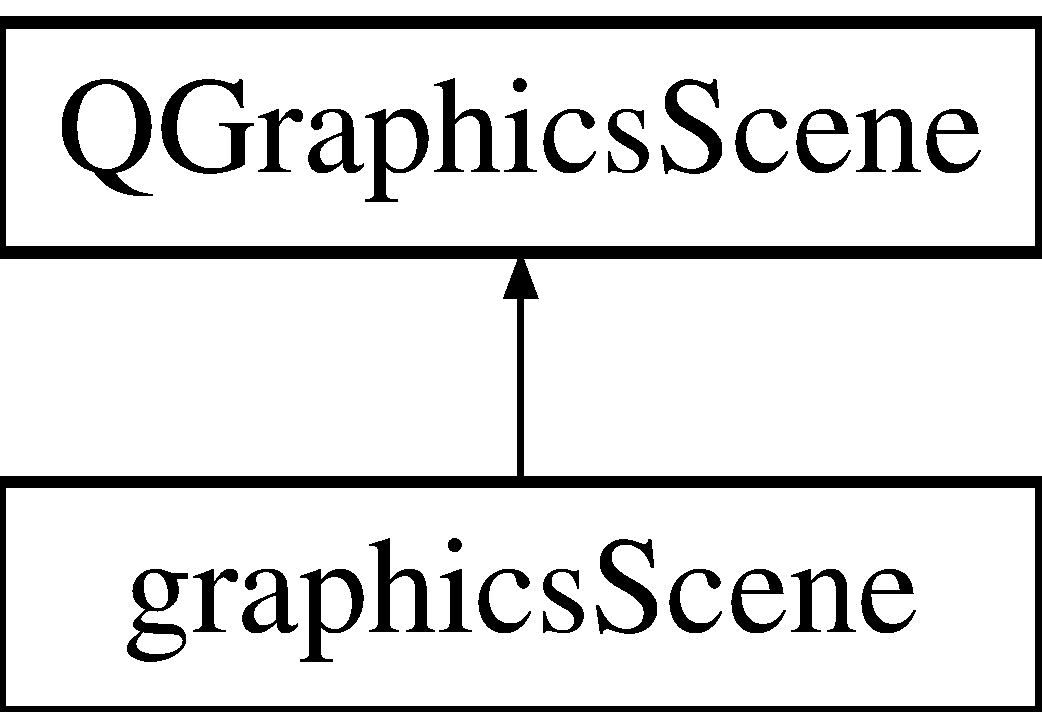
\includegraphics[height=2.000000cm]{classgraphics_scene}
\end{center}
\end{figure}
\subsection*{Signals}
\begin{DoxyCompactItemize}
\item 
\mbox{\Hypertarget{classgraphics_scene_a370117524f759425873aa2dd710958c0}\label{classgraphics_scene_a370117524f759425873aa2dd710958c0}} 
void {\bfseries new\+Mouse\+Left\+Press} (Q\+PointF \mbox{\hyperlink{classpoint}{point}})
\item 
\mbox{\Hypertarget{classgraphics_scene_a788bb2305e72c0deb7cd95a7e245b79a}\label{classgraphics_scene_a788bb2305e72c0deb7cd95a7e245b79a}} 
void {\bfseries new\+Mouse\+Right\+Press} (Q\+PointF \mbox{\hyperlink{classpoint}{point}})
\item 
\mbox{\Hypertarget{classgraphics_scene_ad79f731b826d93f3c84d55f8d411666c}\label{classgraphics_scene_ad79f731b826d93f3c84d55f8d411666c}} 
void {\bfseries new\+Mouse\+Hover} (Q\+PointF \mbox{\hyperlink{classpoint}{point}})
\item 
\mbox{\Hypertarget{classgraphics_scene_ab5dc117c8417d256b4cb9a01cbcd9509}\label{classgraphics_scene_ab5dc117c8417d256b4cb9a01cbcd9509}} 
void {\bfseries un\+Highlight\+Cycle} ()
\end{DoxyCompactItemize}
\subsection*{Public Member Functions}
\begin{DoxyCompactItemize}
\item 
\mbox{\hyperlink{classgraphics_scene_a630f565d827637e6f46f5ae2e786cd06}{graphics\+Scene}} (Q\+Object $\ast$parent=0)
\begin{DoxyCompactList}\small\item\em Scene Constructor. \end{DoxyCompactList}\item 
bool \mbox{\hyperlink{classgraphics_scene_ab84d166160c74279bae4f59c2ccac244}{get\+Point\+Is\+Highlighted}} ()
\begin{DoxyCompactList}\small\item\em \mbox{\hyperlink{classgraphics_scene_ab84d166160c74279bae4f59c2ccac244}{graphics\+Scene\+::get\+Point\+Is\+Highlighted}} getter for point\+Is\+Highlighted. \end{DoxyCompactList}\item 
void \mbox{\hyperlink{classgraphics_scene_a96915f909391e379b8c6c880d1d3acc6}{set\+Point\+Is\+Highlighted}} (const bool \&value)
\begin{DoxyCompactList}\small\item\em \mbox{\hyperlink{classgraphics_scene_a96915f909391e379b8c6c880d1d3acc6}{graphics\+Scene\+::set\+Point\+Is\+Highlighted}} setter for point\+Is\+Highlighted. \end{DoxyCompactList}\item 
virtual void \mbox{\hyperlink{classgraphics_scene_a45ca641319ec6accb1574f52539e7517}{mouse\+Press\+Event}} (Q\+Graphics\+Scene\+Mouse\+Event $\ast$mouse\+Event)
\begin{DoxyCompactList}\small\item\em \mbox{\hyperlink{classgraphics_scene_a45ca641319ec6accb1574f52539e7517}{graphics\+Scene\+::mouse\+Press\+Event}} Mouse pressed on scene \end{DoxyCompactList}\item 
virtual void \mbox{\hyperlink{classgraphics_scene_a08bfd268527873e3bccaa52f34823058}{mouse\+Move\+Event}} (Q\+Graphics\+Scene\+Mouse\+Event $\ast$mouse\+Event)
\begin{DoxyCompactList}\small\item\em \mbox{\hyperlink{classgraphics_scene_a08bfd268527873e3bccaa52f34823058}{graphics\+Scene\+::mouse\+Move\+Event}} Mouse moved on scene. \end{DoxyCompactList}\end{DoxyCompactItemize}


\subsection{Detailed Description}
The \mbox{\hyperlink{classgraphics_scene}{graphics\+Scene}} class. 

Scene displayed in the main part of the G\+UI. 

\subsection{Constructor \& Destructor Documentation}
\mbox{\Hypertarget{classgraphics_scene_a630f565d827637e6f46f5ae2e786cd06}\label{classgraphics_scene_a630f565d827637e6f46f5ae2e786cd06}} 
\index{graphics\+Scene@{graphics\+Scene}!graphics\+Scene@{graphics\+Scene}}
\index{graphics\+Scene@{graphics\+Scene}!graphics\+Scene@{graphics\+Scene}}
\subsubsection{\texorpdfstring{graphics\+Scene()}{graphicsScene()}}
{\footnotesize\ttfamily graphics\+Scene\+::graphics\+Scene (\begin{DoxyParamCaption}\item[{Q\+Object $\ast$}]{parent = {\ttfamily 0} }\end{DoxyParamCaption})\hspace{0.3cm}{\ttfamily [explicit]}}



Scene Constructor. 


\begin{DoxyParams}{Parameters}
{\em parent} & The parent widget to the current widget.\\
\hline
\end{DoxyParams}
Create a new scene setting the scene size to the predetermined size. 

\subsection{Member Function Documentation}
\mbox{\Hypertarget{classgraphics_scene_ab84d166160c74279bae4f59c2ccac244}\label{classgraphics_scene_ab84d166160c74279bae4f59c2ccac244}} 
\index{graphics\+Scene@{graphics\+Scene}!get\+Point\+Is\+Highlighted@{get\+Point\+Is\+Highlighted}}
\index{get\+Point\+Is\+Highlighted@{get\+Point\+Is\+Highlighted}!graphics\+Scene@{graphics\+Scene}}
\subsubsection{\texorpdfstring{get\+Point\+Is\+Highlighted()}{getPointIsHighlighted()}}
{\footnotesize\ttfamily bool graphics\+Scene\+::get\+Point\+Is\+Highlighted (\begin{DoxyParamCaption}{ }\end{DoxyParamCaption})}



\mbox{\hyperlink{classgraphics_scene_ab84d166160c74279bae4f59c2ccac244}{graphics\+Scene\+::get\+Point\+Is\+Highlighted}} getter for point\+Is\+Highlighted. 

\begin{DoxyReturn}{Returns}
bool
\end{DoxyReturn}
Point\+Is\+Highlighted represents a boolean value that determines if a point is being hovered or not. \mbox{\Hypertarget{classgraphics_scene_a08bfd268527873e3bccaa52f34823058}\label{classgraphics_scene_a08bfd268527873e3bccaa52f34823058}} 
\index{graphics\+Scene@{graphics\+Scene}!mouse\+Move\+Event@{mouse\+Move\+Event}}
\index{mouse\+Move\+Event@{mouse\+Move\+Event}!graphics\+Scene@{graphics\+Scene}}
\subsubsection{\texorpdfstring{mouse\+Move\+Event()}{mouseMoveEvent()}}
{\footnotesize\ttfamily void graphics\+Scene\+::mouse\+Move\+Event (\begin{DoxyParamCaption}\item[{Q\+Graphics\+Scene\+Mouse\+Event $\ast$}]{mouse\+Event }\end{DoxyParamCaption})\hspace{0.3cm}{\ttfamily [virtual]}}



\mbox{\hyperlink{classgraphics_scene_a08bfd268527873e3bccaa52f34823058}{graphics\+Scene\+::mouse\+Move\+Event}} Mouse moved on scene. 


\begin{DoxyParams}{Parameters}
{\em mouse\+Event} & Provides information about the mouse event such as the position the click occured on the scene.\\
\hline
\end{DoxyParams}
Called when the mouse moves over the scene. Signal is emitted to update coordinates on the status bar. \mbox{\Hypertarget{classgraphics_scene_a45ca641319ec6accb1574f52539e7517}\label{classgraphics_scene_a45ca641319ec6accb1574f52539e7517}} 
\index{graphics\+Scene@{graphics\+Scene}!mouse\+Press\+Event@{mouse\+Press\+Event}}
\index{mouse\+Press\+Event@{mouse\+Press\+Event}!graphics\+Scene@{graphics\+Scene}}
\subsubsection{\texorpdfstring{mouse\+Press\+Event()}{mousePressEvent()}}
{\footnotesize\ttfamily void graphics\+Scene\+::mouse\+Press\+Event (\begin{DoxyParamCaption}\item[{Q\+Graphics\+Scene\+Mouse\+Event $\ast$}]{mouse\+Event }\end{DoxyParamCaption})\hspace{0.3cm}{\ttfamily [virtual]}}



\mbox{\hyperlink{classgraphics_scene_a45ca641319ec6accb1574f52539e7517}{graphics\+Scene\+::mouse\+Press\+Event}} Mouse pressed on scene 


\begin{DoxyParams}{Parameters}
{\em mouse\+Event} & Provides information about the mouse event such as the position the click occured on the scene.\\
\hline
\end{DoxyParams}
Called when the mouse button is clicked on the scene in the graphics view. A left mouse click will mean a new point is created or the highlighted point is moved. A right mouse click will display the context menu. \mbox{\Hypertarget{classgraphics_scene_a96915f909391e379b8c6c880d1d3acc6}\label{classgraphics_scene_a96915f909391e379b8c6c880d1d3acc6}} 
\index{graphics\+Scene@{graphics\+Scene}!set\+Point\+Is\+Highlighted@{set\+Point\+Is\+Highlighted}}
\index{set\+Point\+Is\+Highlighted@{set\+Point\+Is\+Highlighted}!graphics\+Scene@{graphics\+Scene}}
\subsubsection{\texorpdfstring{set\+Point\+Is\+Highlighted()}{setPointIsHighlighted()}}
{\footnotesize\ttfamily void graphics\+Scene\+::set\+Point\+Is\+Highlighted (\begin{DoxyParamCaption}\item[{const bool \&}]{value }\end{DoxyParamCaption})}



\mbox{\hyperlink{classgraphics_scene_a96915f909391e379b8c6c880d1d3acc6}{graphics\+Scene\+::set\+Point\+Is\+Highlighted}} setter for point\+Is\+Highlighted. 


\begin{DoxyParams}{Parameters}
{\em value} & Point\+Is\+Highlighted represents a boolean value that determines if a point is being hovered or not. \\
\hline
\end{DoxyParams}


The documentation for this class was generated from the following files\+:\begin{DoxyCompactItemize}
\item 
/\+Users/lukehutton/\+One\+Drive -\/ University of Leeds/\+University/\+Computer Science/\+Internship/moebinv-\/gui/include/scene.\+h\item 
/\+Users/lukehutton/\+One\+Drive -\/ University of Leeds/\+University/\+Computer Science/\+Internship/moebinv-\/gui/moebinv-\/gui-\/build/moc\+\_\+scene.\+cpp\item 
/\+Users/lukehutton/\+One\+Drive -\/ University of Leeds/\+University/\+Computer Science/\+Internship/moebinv-\/gui/src/scene.\+cpp\end{DoxyCompactItemize}

\hypertarget{classhelp_browser}{}\section{help\+Browser Class Reference}
\label{classhelp_browser}\index{help\+Browser@{help\+Browser}}
Inheritance diagram for help\+Browser\+:\begin{figure}[H]
\begin{center}
\leavevmode
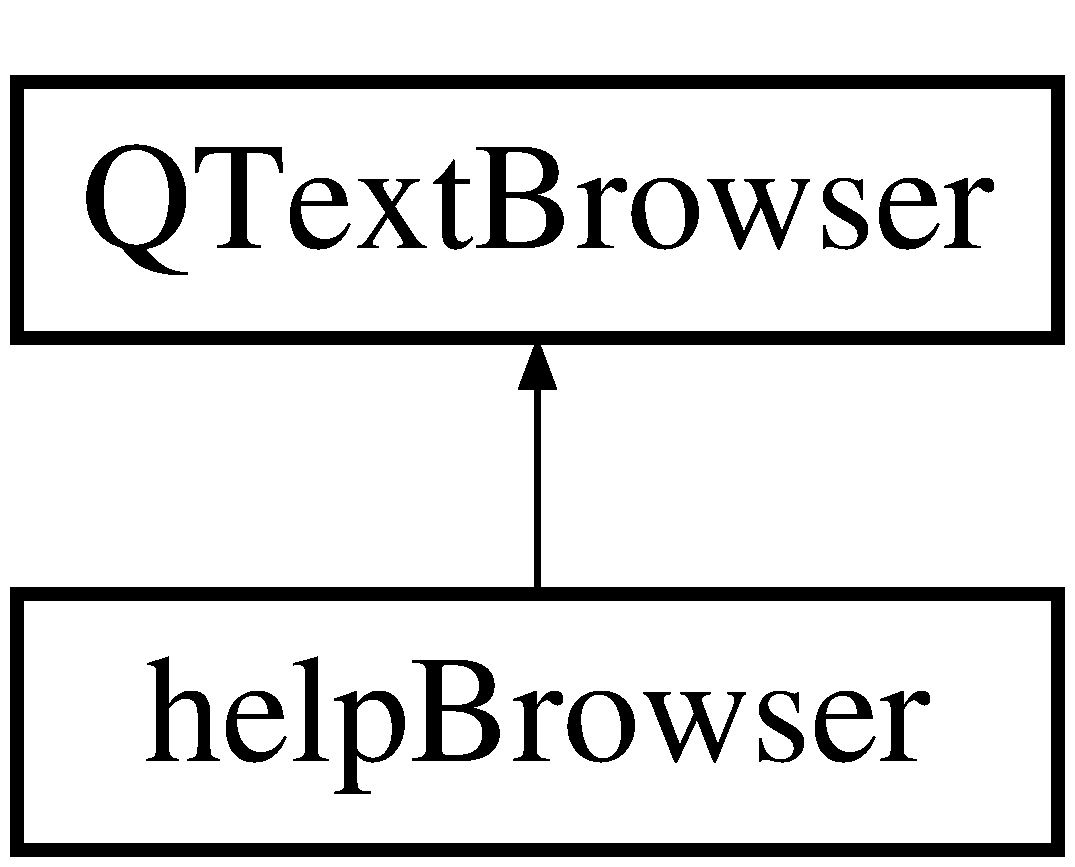
\includegraphics[height=2.000000cm]{classhelp_browser}
\end{center}
\end{figure}
\subsection*{Public Member Functions}
\begin{DoxyCompactItemize}
\item 
\mbox{\Hypertarget{classhelp_browser_a0c24d5dbf041a323695a9260c1f4d774}\label{classhelp_browser_a0c24d5dbf041a323695a9260c1f4d774}} 
{\bfseries help\+Browser} (Q\+Widget $\ast$parent=0, Q\+Help\+Engine $\ast$help\+Engine=nullptr)
\item 
\mbox{\Hypertarget{classhelp_browser_a92edbf57806761e03457bf941587c2a8}\label{classhelp_browser_a92edbf57806761e03457bf941587c2a8}} 
Q\+Variant {\bfseries load\+Resource} (int type, const Q\+Url \&name)
\item 
\mbox{\Hypertarget{classhelp_browser_a2ecdeeeeca618d3436adeec6d782f621}\label{classhelp_browser_a2ecdeeeeca618d3436adeec6d782f621}} 
void {\bfseries set\+Help\+Engine} (Q\+Help\+Engine $\ast$help\+Engine)
\end{DoxyCompactItemize}


The documentation for this class was generated from the following files\+:\begin{DoxyCompactItemize}
\item 
/\+Users/lukehutton/\+One\+Drive -\/ University of Leeds/\+University/\+Computer Science/\+Internship/moebinv-\/gui/include/helpdialog.\+h\item 
/\+Users/lukehutton/\+One\+Drive -\/ University of Leeds/\+University/\+Computer Science/\+Internship/moebinv-\/gui/src/helpdialog.\+cpp\end{DoxyCompactItemize}

\hypertarget{class_ui_1_1help_dialog}{}\section{Ui\+:\+:help\+Dialog Class Reference}
\label{class_ui_1_1help_dialog}\index{Ui\+::help\+Dialog@{Ui\+::help\+Dialog}}
Inheritance diagram for Ui\+:\+:help\+Dialog\+:\begin{figure}[H]
\begin{center}
\leavevmode
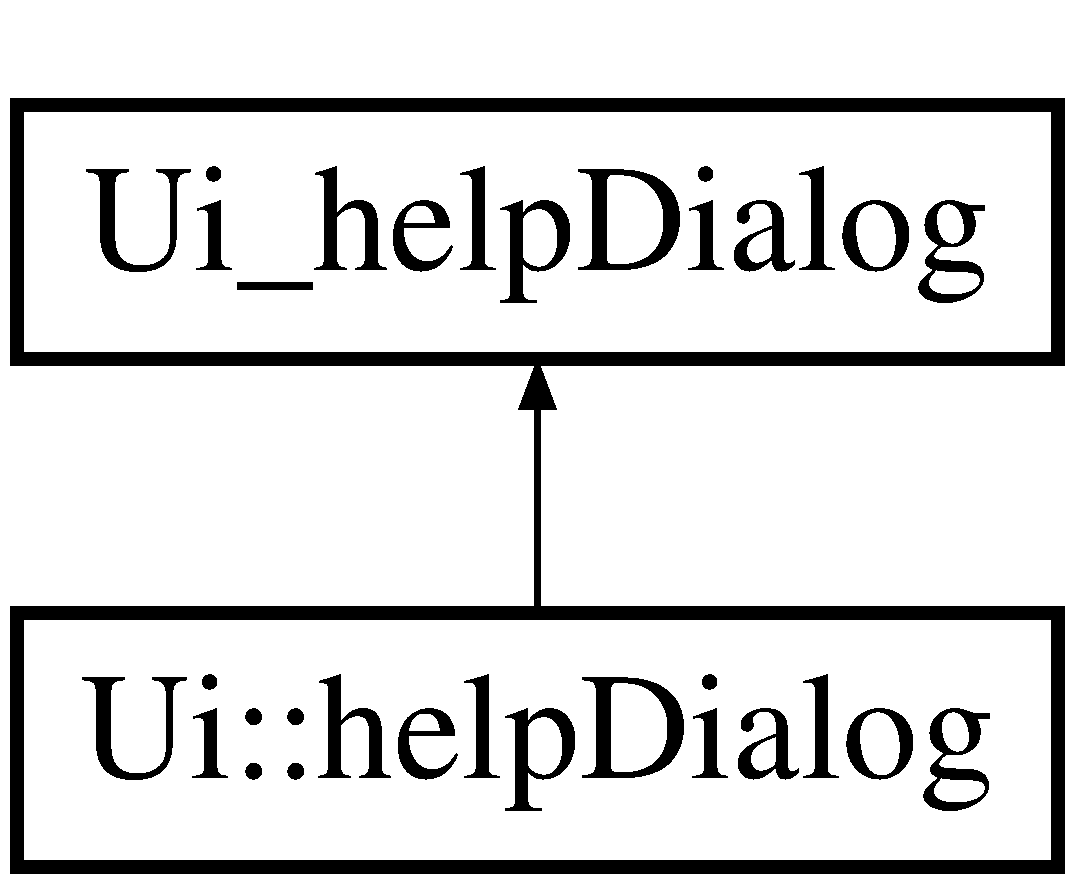
\includegraphics[height=2.000000cm]{class_ui_1_1help_dialog}
\end{center}
\end{figure}
\subsection*{Additional Inherited Members}


The documentation for this class was generated from the following file\+:\begin{DoxyCompactItemize}
\item 
/\+Users/lukehutton/\+One\+Drive -\/ University of Leeds/\+University/\+Computer Science/\+Internship/moebinv-\/gui/moebinv-\/gui-\/build/ui\+\_\+helpdialog.\+h\end{DoxyCompactItemize}

\hypertarget{classhelp_dialog}{}\section{help\+Dialog Class Reference}
\label{classhelp_dialog}\index{help\+Dialog@{help\+Dialog}}
Inheritance diagram for help\+Dialog\+:\begin{figure}[H]
\begin{center}
\leavevmode
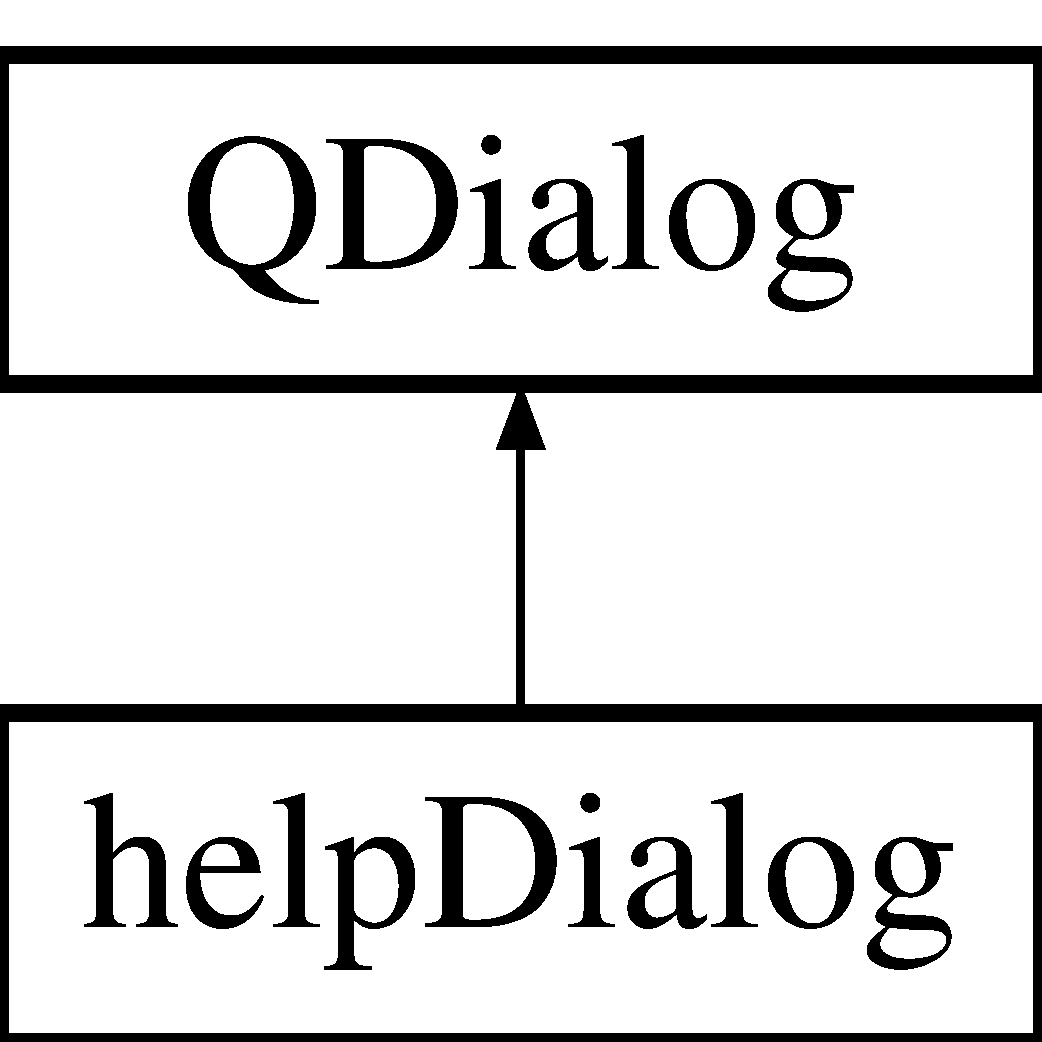
\includegraphics[height=2.000000cm]{classhelp_dialog}
\end{center}
\end{figure}
\subsection*{Public Member Functions}
\begin{DoxyCompactItemize}
\item 
\mbox{\Hypertarget{classhelp_dialog_a84aceebf9a77e5c6afc9842b212d0961}\label{classhelp_dialog_a84aceebf9a77e5c6afc9842b212d0961}} 
{\bfseries help\+Dialog} (Q\+Widget $\ast$parent=0)
\end{DoxyCompactItemize}


The documentation for this class was generated from the following files\+:\begin{DoxyCompactItemize}
\item 
/\+Users/lukehutton/\+One\+Drive -\/ University of Leeds/\+University/\+Computer Science/\+Internship/moebinv-\/gui/include/helpdialog.\+h\item 
/\+Users/lukehutton/\+One\+Drive -\/ University of Leeds/\+University/\+Computer Science/\+Internship/moebinv-\/gui/src/helpdialog.\+cpp\end{DoxyCompactItemize}

\hypertarget{structid_dist}{}\section{id\+Dist Struct Reference}
\label{structid_dist}\index{id\+Dist@{id\+Dist}}


{\ttfamily \#include $<$vis.\+h$>$}

\subsection*{Public Attributes}
\begin{DoxyCompactItemize}
\item 
int \mbox{\hyperlink{structid_dist_a444479adc980289189d07fc2303ab9f6}{id}}
\item 
double \mbox{\hyperlink{structid_dist_ab4b00d9dbea04e198c67ad6ada5f881c}{dist}}
\end{DoxyCompactItemize}


\subsection{Detailed Description}
a structure that contains an id and distance from plane value. used for sorting translucent objects. 

\subsection{Member Data Documentation}
\mbox{\Hypertarget{structid_dist_ab4b00d9dbea04e198c67ad6ada5f881c}\label{structid_dist_ab4b00d9dbea04e198c67ad6ada5f881c}} 
\index{id\+Dist@{id\+Dist}!dist@{dist}}
\index{dist@{dist}!id\+Dist@{id\+Dist}}
\subsubsection{\texorpdfstring{dist}{dist}}
{\footnotesize\ttfamily double id\+Dist\+::dist}

distance from plane parallel to camera through origin. \mbox{\Hypertarget{structid_dist_a444479adc980289189d07fc2303ab9f6}\label{structid_dist_a444479adc980289189d07fc2303ab9f6}} 
\index{id\+Dist@{id\+Dist}!id@{id}}
\index{id@{id}!id\+Dist@{id\+Dist}}
\subsubsection{\texorpdfstring{id}{id}}
{\footnotesize\ttfamily int id\+Dist\+::id}

id value of object for which distance has been computed. 

The documentation for this struct was generated from the following file\+:\begin{DoxyCompactItemize}
\item 
/\+Users/lukehutton/\+One\+Drive -\/ University of Leeds/\+University/\+Computer Science/\+Internship/moebinv-\/gui/lib/moebinv-\/3.\+2/cycle3\+D-\/visualiser/vis.\+h\end{DoxyCompactItemize}

\hypertarget{structid_over_vec_len}{}\section{id\+Over\+Vec\+Len Struct Reference}
\label{structid_over_vec_len}\index{id\+Over\+Vec\+Len@{id\+Over\+Vec\+Len}}


{\ttfamily \#include $<$vis.\+h$>$}

\subsection*{Public Attributes}
\begin{DoxyCompactItemize}
\item 
int \mbox{\hyperlink{structid_over_vec_len_ac728d62d94bf608a6f11ce5c0a6485ad}{id}}
\item 
double \mbox{\hyperlink{structid_over_vec_len_a9387d2c3130328e5e24988d759f5a46a}{over}}
\item 
\mbox{\hyperlink{struct_point}{Point}} \mbox{\hyperlink{structid_over_vec_len_a86fea6b0e81e2e4addb46265dd570985}{vec}}
\item 
double \mbox{\hyperlink{structid_over_vec_len_ac78dfd24fef77a3e5a90d2c3c4576548}{len}}
\end{DoxyCompactItemize}


\subsection{Detailed Description}
structure that contains an id, overlap distance, direction vector and length. used for sorting storing intersection details between two objects. 

\subsection{Member Data Documentation}
\mbox{\Hypertarget{structid_over_vec_len_ac728d62d94bf608a6f11ce5c0a6485ad}\label{structid_over_vec_len_ac728d62d94bf608a6f11ce5c0a6485ad}} 
\index{id\+Over\+Vec\+Len@{id\+Over\+Vec\+Len}!id@{id}}
\index{id@{id}!id\+Over\+Vec\+Len@{id\+Over\+Vec\+Len}}
\subsubsection{\texorpdfstring{id}{id}}
{\footnotesize\ttfamily int id\+Over\+Vec\+Len\+::id}

id value of object that intersects object we are working with. \mbox{\Hypertarget{structid_over_vec_len_ac78dfd24fef77a3e5a90d2c3c4576548}\label{structid_over_vec_len_ac78dfd24fef77a3e5a90d2c3c4576548}} 
\index{id\+Over\+Vec\+Len@{id\+Over\+Vec\+Len}!len@{len}}
\index{len@{len}!id\+Over\+Vec\+Len@{id\+Over\+Vec\+Len}}
\subsubsection{\texorpdfstring{len}{len}}
{\footnotesize\ttfamily double id\+Over\+Vec\+Len\+::len}

distance between centre of both objects. \mbox{\Hypertarget{structid_over_vec_len_a9387d2c3130328e5e24988d759f5a46a}\label{structid_over_vec_len_a9387d2c3130328e5e24988d759f5a46a}} 
\index{id\+Over\+Vec\+Len@{id\+Over\+Vec\+Len}!over@{over}}
\index{over@{over}!id\+Over\+Vec\+Len@{id\+Over\+Vec\+Len}}
\subsubsection{\texorpdfstring{over}{over}}
{\footnotesize\ttfamily double id\+Over\+Vec\+Len\+::over}

overlap, sum of their radii -\/ distance between them. \mbox{\Hypertarget{structid_over_vec_len_a86fea6b0e81e2e4addb46265dd570985}\label{structid_over_vec_len_a86fea6b0e81e2e4addb46265dd570985}} 
\index{id\+Over\+Vec\+Len@{id\+Over\+Vec\+Len}!vec@{vec}}
\index{vec@{vec}!id\+Over\+Vec\+Len@{id\+Over\+Vec\+Len}}
\subsubsection{\texorpdfstring{vec}{vec}}
{\footnotesize\ttfamily \mbox{\hyperlink{struct_point}{Point}} id\+Over\+Vec\+Len\+::vec}

direction vector from object we\textquotesingle{}re working with\textquotesingle{}s centre to id\textquotesingle{}s centre. 

The documentation for this struct was generated from the following file\+:\begin{DoxyCompactItemize}
\item 
/\+Users/lukehutton/\+One\+Drive -\/ University of Leeds/\+University/\+Computer Science/\+Internship/moebinv-\/gui/lib/moebinv-\/3.\+2/cycle3\+D-\/visualiser/vis.\+h\end{DoxyCompactItemize}

\hypertarget{structint_draw}{}\section{int\+Draw Struct Reference}
\label{structint_draw}\index{int\+Draw@{int\+Draw}}


{\ttfamily \#include $<$vis.\+h$>$}

\subsection*{Public Attributes}
\begin{DoxyCompactItemize}
\item 
\mbox{\hyperlink{struct_point}{Point}} \mbox{\hyperlink{structint_draw_af1dad79cd2a2fd363e908b413bbbc128}{cen}}
\item 
\mbox{\hyperlink{struct_point}{Point}} \mbox{\hyperlink{structint_draw_a527717b140f7983792ea0baeb1a3f234}{vec}}
\item 
double \mbox{\hyperlink{structint_draw_a9614ba917e8a2c0f7b782b72d12ba67b}{rad}}
\item 
int \mbox{\hyperlink{structint_draw_a96bf5f7cd19d3a83bd5a53f2fa0aeb71}{id1}}
\item 
int \mbox{\hyperlink{structint_draw_a25ba59d3175591863f4e240e4fe6bd13}{id2}}
\end{DoxyCompactItemize}


\subsection{Detailed Description}
structure to store data about a particular intersection, including circle of intersection details, vector between the two spheres, and the ids of the two spheres involved. Used for drawing intersections. 

\subsection{Member Data Documentation}
\mbox{\Hypertarget{structint_draw_af1dad79cd2a2fd363e908b413bbbc128}\label{structint_draw_af1dad79cd2a2fd363e908b413bbbc128}} 
\index{int\+Draw@{int\+Draw}!cen@{cen}}
\index{cen@{cen}!int\+Draw@{int\+Draw}}
\subsubsection{\texorpdfstring{cen}{cen}}
{\footnotesize\ttfamily \mbox{\hyperlink{struct_point}{Point}} int\+Draw\+::cen}

centre of circle of intersection. \mbox{\Hypertarget{structint_draw_a96bf5f7cd19d3a83bd5a53f2fa0aeb71}\label{structint_draw_a96bf5f7cd19d3a83bd5a53f2fa0aeb71}} 
\index{int\+Draw@{int\+Draw}!id1@{id1}}
\index{id1@{id1}!int\+Draw@{int\+Draw}}
\subsubsection{\texorpdfstring{id1}{id1}}
{\footnotesize\ttfamily int int\+Draw\+::id1}

id of one object involved in intersection. \mbox{\Hypertarget{structint_draw_a25ba59d3175591863f4e240e4fe6bd13}\label{structint_draw_a25ba59d3175591863f4e240e4fe6bd13}} 
\index{int\+Draw@{int\+Draw}!id2@{id2}}
\index{id2@{id2}!int\+Draw@{int\+Draw}}
\subsubsection{\texorpdfstring{id2}{id2}}
{\footnotesize\ttfamily int int\+Draw\+::id2}

id of other object involved in intersection. \mbox{\Hypertarget{structint_draw_a9614ba917e8a2c0f7b782b72d12ba67b}\label{structint_draw_a9614ba917e8a2c0f7b782b72d12ba67b}} 
\index{int\+Draw@{int\+Draw}!rad@{rad}}
\index{rad@{rad}!int\+Draw@{int\+Draw}}
\subsubsection{\texorpdfstring{rad}{rad}}
{\footnotesize\ttfamily double int\+Draw\+::rad}

radius of circle of intersection. \mbox{\Hypertarget{structint_draw_a527717b140f7983792ea0baeb1a3f234}\label{structint_draw_a527717b140f7983792ea0baeb1a3f234}} 
\index{int\+Draw@{int\+Draw}!vec@{vec}}
\index{vec@{vec}!int\+Draw@{int\+Draw}}
\subsubsection{\texorpdfstring{vec}{vec}}
{\footnotesize\ttfamily \mbox{\hyperlink{struct_point}{Point}} int\+Draw\+::vec}

orthogonal vector to circle of intersection. 

The documentation for this struct was generated from the following file\+:\begin{DoxyCompactItemize}
\item 
/\+Users/lukehutton/\+One\+Drive -\/ University of Leeds/\+University/\+Computer Science/\+Internship/moebinv-\/gui/lib/moebinv-\/3.\+2/cycle3\+D-\/visualiser/vis.\+h\end{DoxyCompactItemize}

\hypertarget{structint_pair}{}\section{int\+Pair Struct Reference}
\label{structint_pair}\index{int\+Pair@{int\+Pair}}


{\ttfamily \#include $<$vis.\+h$>$}

\subsection*{Public Attributes}
\begin{DoxyCompactItemize}
\item 
int \mbox{\hyperlink{structint_pair_ab5871710162bfd837cbb99e4645e7662}{x}}
\item 
int \mbox{\hyperlink{structint_pair_a88f4c4355f1c525696998cb8e69fa285}{y}}
\end{DoxyCompactItemize}


\subsection{Detailed Description}
stores 2 integers. used when pair cannot be used ie. for non-\/compile-\/time constants 

\subsection{Member Data Documentation}
\mbox{\Hypertarget{structint_pair_ab5871710162bfd837cbb99e4645e7662}\label{structint_pair_ab5871710162bfd837cbb99e4645e7662}} 
\index{int\+Pair@{int\+Pair}!x@{x}}
\index{x@{x}!int\+Pair@{int\+Pair}}
\subsubsection{\texorpdfstring{x}{x}}
{\footnotesize\ttfamily int int\+Pair\+::x}

first integer of pair. \mbox{\Hypertarget{structint_pair_a88f4c4355f1c525696998cb8e69fa285}\label{structint_pair_a88f4c4355f1c525696998cb8e69fa285}} 
\index{int\+Pair@{int\+Pair}!y@{y}}
\index{y@{y}!int\+Pair@{int\+Pair}}
\subsubsection{\texorpdfstring{y}{y}}
{\footnotesize\ttfamily int int\+Pair\+::y}

second integer of pair. 

The documentation for this struct was generated from the following file\+:\begin{DoxyCompactItemize}
\item 
/\+Users/lukehutton/\+One\+Drive -\/ University of Leeds/\+University/\+Computer Science/\+Internship/moebinv-\/gui/lib/moebinv-\/3.\+2/cycle3\+D-\/visualiser/vis.\+h\end{DoxyCompactItemize}

\hypertarget{classlabels}{}\section{labels Class Reference}
\label{classlabels}\index{labels@{labels}}


The labels class.  




{\ttfamily \#include $<$labels.\+h$>$}

\subsection*{Public Member Functions}
\begin{DoxyCompactItemize}
\item 
\mbox{\Hypertarget{classlabels_aabee553ffee5eb33826c90bbda2dbc58}\label{classlabels_aabee553ffee5eb33826c90bbda2dbc58}} 
\mbox{\hyperlink{classlabels_aabee553ffee5eb33826c90bbda2dbc58}{labels}} ()
\begin{DoxyCompactList}\small\item\em \mbox{\hyperlink{classlabels_aabee553ffee5eb33826c90bbda2dbc58}{labels\+::labels}} Labels constructor. \end{DoxyCompactList}\item 
Q\+String \mbox{\hyperlink{classlabels_a70a7436dbef91e342fec4ec3130187e2}{gen\+Next\+Label}} ()
\begin{DoxyCompactList}\small\item\em \mbox{\hyperlink{classlabels_a70a7436dbef91e342fec4ec3130187e2}{labels\+::gen\+Next\+Label}} Generate next label. \end{DoxyCompactList}\item 
\mbox{\Hypertarget{classlabels_a790344f0c86546b9b5fdda30dbe690a5}\label{classlabels_a790344f0c86546b9b5fdda30dbe690a5}} 
void {\bfseries advance\+Label} ()
\end{DoxyCompactItemize}


\subsection{Detailed Description}
The labels class. 

The labels class is a small class which generates a unique label incrementing as such\+: A, B, C, ..., Z, AA, AB, ... ZZ, A\+AA, ect... 

\subsection{Member Function Documentation}
\mbox{\Hypertarget{classlabels_a70a7436dbef91e342fec4ec3130187e2}\label{classlabels_a70a7436dbef91e342fec4ec3130187e2}} 
\index{labels@{labels}!gen\+Next\+Label@{gen\+Next\+Label}}
\index{gen\+Next\+Label@{gen\+Next\+Label}!labels@{labels}}
\subsubsection{\texorpdfstring{gen\+Next\+Label()}{genNextLabel()}}
{\footnotesize\ttfamily Q\+String labels\+::gen\+Next\+Label (\begin{DoxyParamCaption}{ }\end{DoxyParamCaption})}



\mbox{\hyperlink{classlabels_a70a7436dbef91e342fec4ec3130187e2}{labels\+::gen\+Next\+Label}} Generate next label. 

\begin{DoxyReturn}{Returns}
New label.
\end{DoxyReturn}
Generate the next label in the sequence i.\+e. A, B, C, ..., Z, AA, AB, ... 

The documentation for this class was generated from the following files\+:\begin{DoxyCompactItemize}
\item 
/\+Users/lukehutton/\+One\+Drive -\/ University of Leeds/\+University/\+Computer Science/\+Internship/moebinv-\/gui/include/labels.\+h\item 
/\+Users/lukehutton/\+One\+Drive -\/ University of Leeds/\+University/\+Computer Science/\+Internship/moebinv-\/gui/src/labels.\+cpp\end{DoxyCompactItemize}

\hypertarget{classline}{}\section{line Class Reference}
\label{classline}\index{line@{line}}
Inheritance diagram for line\+:\begin{figure}[H]
\begin{center}
\leavevmode
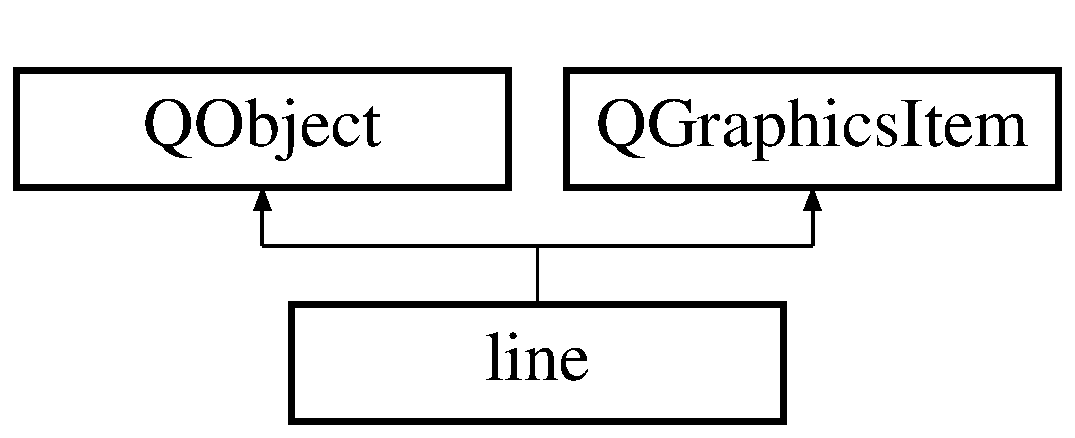
\includegraphics[height=2.000000cm]{classline}
\end{center}
\end{figure}
\subsection*{Public Member Functions}
\begin{DoxyCompactItemize}
\item 
\mbox{\hyperlink{classline_a38ef6d493f122a35237517bc79653821}{line}} (\mbox{\hyperlink{classgraphic_cycle}{graphic\+Cycle}} $\ast$parent, struct \mbox{\hyperlink{structcycle_data}{cycle\+Data}} data)
\begin{DoxyCompactList}\small\item\em \mbox{\hyperlink{classline_a38ef6d493f122a35237517bc79653821}{line\+::line}} Create a new line. \end{DoxyCompactList}\item 
void \mbox{\hyperlink{classline_a128cee38b49baa22b618165edc900e81}{paint}} (Q\+Painter $\ast$painter, const Q\+Style\+Option\+Graphics\+Item $\ast$option, Q\+Widget $\ast$widget)
\begin{DoxyCompactList}\small\item\em \mbox{\hyperlink{classline_a128cee38b49baa22b618165edc900e81}{line\+::paint}} Paint the point on the scene. \end{DoxyCompactList}\item 
Q\+RectF \mbox{\hyperlink{classline_aecbda133a991abe5bb4080416c226e2f}{bounding\+Rect}} () const
\begin{DoxyCompactList}\small\item\em \mbox{\hyperlink{classline_aecbda133a991abe5bb4080416c226e2f}{line\+::bounding\+Rect}} Define the bounding rect. \end{DoxyCompactList}\item 
void \mbox{\hyperlink{classline_a0638608cbb7231dc4a55ea795e367748}{find\+Line\+Points}} ()
\begin{DoxyCompactList}\small\item\em line\+::shape Define the clipping mask of the object \end{DoxyCompactList}\end{DoxyCompactItemize}


\subsection{Constructor \& Destructor Documentation}
\mbox{\Hypertarget{classline_a38ef6d493f122a35237517bc79653821}\label{classline_a38ef6d493f122a35237517bc79653821}} 
\index{line@{line}!line@{line}}
\index{line@{line}!line@{line}}
\subsubsection{\texorpdfstring{line()}{line()}}
{\footnotesize\ttfamily line\+::line (\begin{DoxyParamCaption}\item[{\mbox{\hyperlink{classgraphic_cycle}{graphic\+Cycle}} $\ast$}]{parent,  }\item[{struct \mbox{\hyperlink{structcycle_data}{cycle\+Data}}}]{data }\end{DoxyParamCaption})}



\mbox{\hyperlink{classline_a38ef6d493f122a35237517bc79653821}{line\+::line}} Create a new line. 


\begin{DoxyParams}{Parameters}
{\em struct} & \mbox{\hyperlink{structcycle_data}{cycle\+Data}} data Contains the data needed to draw the line.\\
\hline
\end{DoxyParams}
Construct a new line on the scene and assign it to the parent \mbox{\hyperlink{classgraphic_cycle}{graphic\+Cycle}}. 

\subsection{Member Function Documentation}
\mbox{\Hypertarget{classline_aecbda133a991abe5bb4080416c226e2f}\label{classline_aecbda133a991abe5bb4080416c226e2f}} 
\index{line@{line}!bounding\+Rect@{bounding\+Rect}}
\index{bounding\+Rect@{bounding\+Rect}!line@{line}}
\subsubsection{\texorpdfstring{bounding\+Rect()}{boundingRect()}}
{\footnotesize\ttfamily Q\+RectF line\+::bounding\+Rect (\begin{DoxyParamCaption}{ }\end{DoxyParamCaption}) const}



\mbox{\hyperlink{classline_aecbda133a991abe5bb4080416c226e2f}{line\+::bounding\+Rect}} Define the bounding rect. 

\begin{DoxyReturn}{Returns}
Q\+RectF
\end{DoxyReturn}
Define the box the object is drawn within on the scene. \mbox{\Hypertarget{classline_a0638608cbb7231dc4a55ea795e367748}\label{classline_a0638608cbb7231dc4a55ea795e367748}} 
\index{line@{line}!find\+Line\+Points@{find\+Line\+Points}}
\index{find\+Line\+Points@{find\+Line\+Points}!line@{line}}
\subsubsection{\texorpdfstring{find\+Line\+Points()}{findLinePoints()}}
{\footnotesize\ttfamily void line\+::find\+Line\+Points (\begin{DoxyParamCaption}{ }\end{DoxyParamCaption})}



line\+::shape Define the clipping mask of the object 

\begin{DoxyReturn}{Returns}
Q\+Painter\+Path
\end{DoxyReturn}
Defines the area in which the shape actually exists.

\mbox{\hyperlink{classline_a0638608cbb7231dc4a55ea795e367748}{line\+::find\+Line\+Points}} Find the points\+: (x1, y1), (x2, y2).

This function finds the two points in which the line will be drawn between. Hence since we need to draw a line accross the whole of the scene, we find two points which are beyond the scene and draw the line between those. \mbox{\Hypertarget{classline_a128cee38b49baa22b618165edc900e81}\label{classline_a128cee38b49baa22b618165edc900e81}} 
\index{line@{line}!paint@{paint}}
\index{paint@{paint}!line@{line}}
\subsubsection{\texorpdfstring{paint()}{paint()}}
{\footnotesize\ttfamily void line\+::paint (\begin{DoxyParamCaption}\item[{Q\+Painter $\ast$}]{painter,  }\item[{const Q\+Style\+Option\+Graphics\+Item $\ast$}]{option,  }\item[{Q\+Widget $\ast$}]{widget }\end{DoxyParamCaption})}



\mbox{\hyperlink{classline_a128cee38b49baa22b618165edc900e81}{line\+::paint}} Paint the point on the scene. 


\begin{DoxyParams}{Parameters}
{\em p} & Q\+Painter object. \\
\hline
{\em option} & \\
\hline
{\em widget} & This function paints the line on the scene given various parameters (such as x and y). The line is drawn differently dependent on the drawing metric in use. \\
\hline
\end{DoxyParams}


The documentation for this class was generated from the following files\+:\begin{DoxyCompactItemize}
\item 
/\+Users/lukehutton/\+One\+Drive -\/ University of Leeds/\+University/\+Computer Science/\+Internship/moebinv-\/gui/include/line.\+h\item 
/\+Users/lukehutton/\+One\+Drive -\/ University of Leeds/\+University/\+Computer Science/\+Internship/moebinv-\/gui/src/line.\+cpp\end{DoxyCompactItemize}

\hypertarget{class_ui_1_1_main_window}{}\section{Ui\+:\+:Main\+Window Class Reference}
\label{class_ui_1_1_main_window}\index{Ui\+::\+Main\+Window@{Ui\+::\+Main\+Window}}
Inheritance diagram for Ui\+:\+:Main\+Window\+:\begin{figure}[H]
\begin{center}
\leavevmode
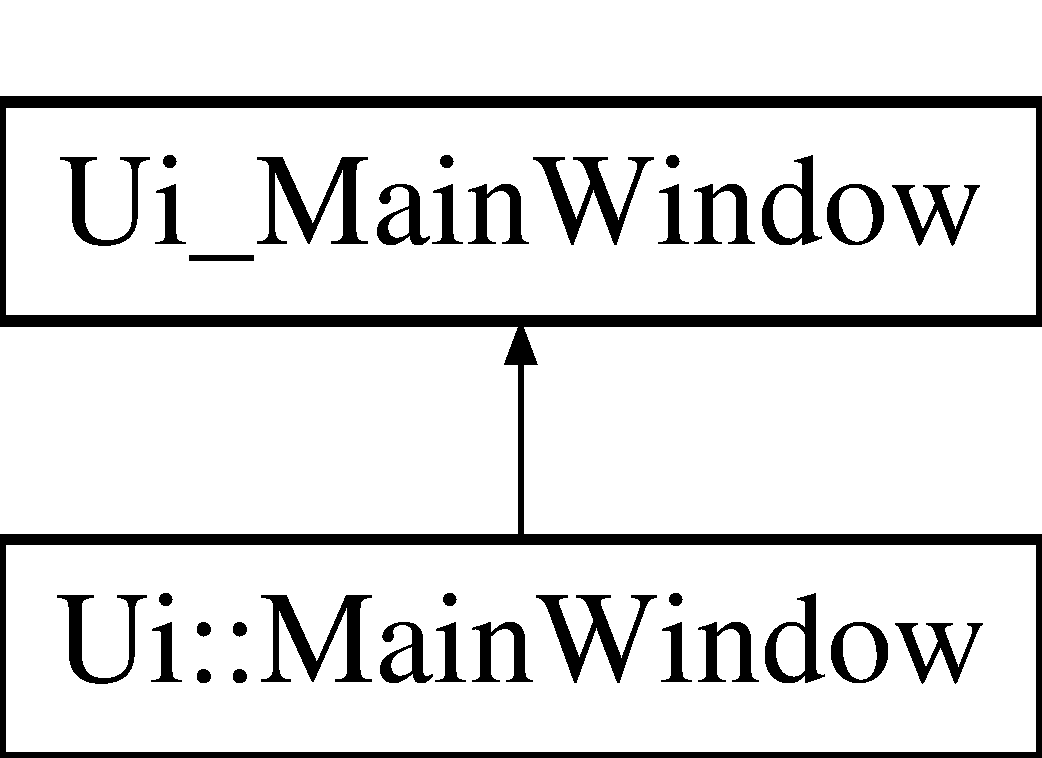
\includegraphics[height=2.000000cm]{class_ui_1_1_main_window}
\end{center}
\end{figure}
\subsection*{Additional Inherited Members}


The documentation for this class was generated from the following file\+:\begin{DoxyCompactItemize}
\item 
/\+Users/lukehutton/\+One\+Drive -\/ University of Leeds/\+University/\+Computer Science/\+Internship/moebinv-\/gui/moebinv-\/gui-\/build/ui\+\_\+mainwindow.\+h\end{DoxyCompactItemize}

\hypertarget{class_main_window}{}\section{Main\+Window Class Reference}
\label{class_main_window}\index{Main\+Window@{Main\+Window}}


The \mbox{\hyperlink{class_main_window}{Main\+Window}} class.  




{\ttfamily \#include $<$mainwindow.\+h$>$}

Inheritance diagram for Main\+Window\+:\begin{figure}[H]
\begin{center}
\leavevmode
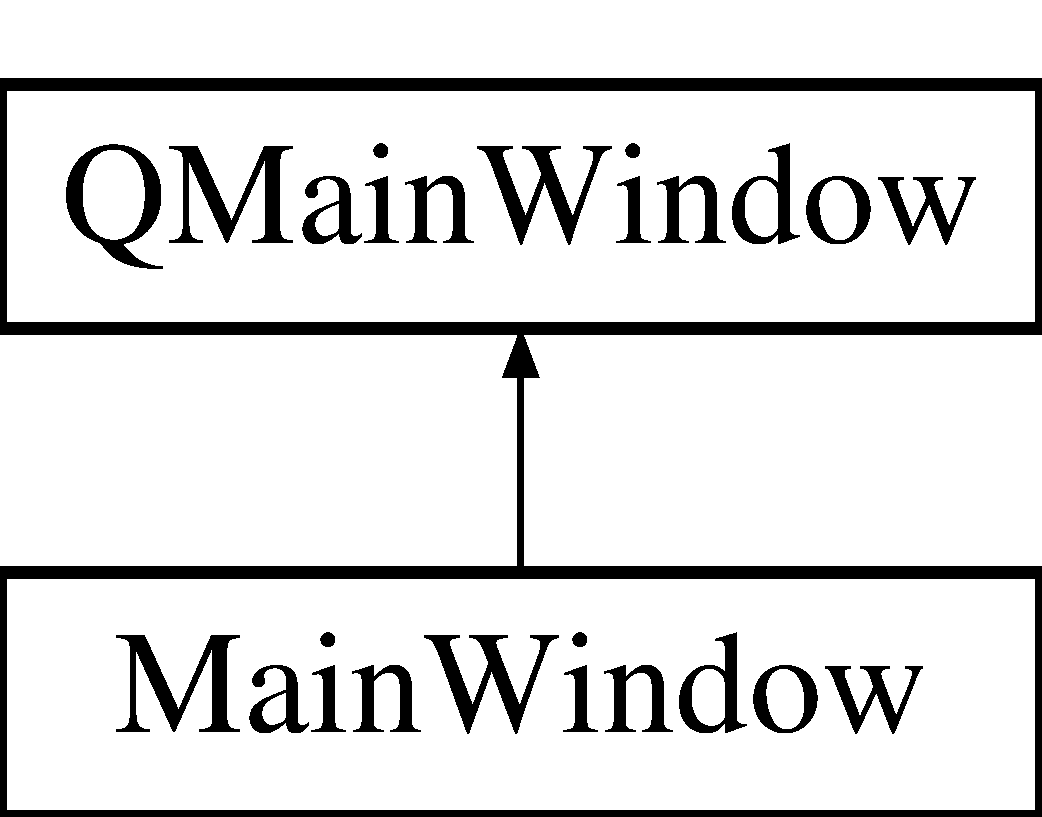
\includegraphics[height=2.000000cm]{class_main_window}
\end{center}
\end{figure}
\subsection*{Signals}
\begin{DoxyCompactItemize}
\item 
\mbox{\Hypertarget{class_main_window_a46ebd786b1aeb0ef026f0a3f32dd9f3d}\label{class_main_window_a46ebd786b1aeb0ef026f0a3f32dd9f3d}} 
void {\bfseries reset\+Relational\+List} ()
\end{DoxyCompactItemize}
\subsection*{Public Member Functions}
\begin{DoxyCompactItemize}
\item 
\mbox{\hyperlink{class_main_window_a8b244be8b7b7db1b08de2a2acb9409db}{Main\+Window}} (Q\+Widget $\ast$parent=0)
\begin{DoxyCompactList}\small\item\em \mbox{\hyperlink{class_main_window_a8b244be8b7b7db1b08de2a2acb9409db}{Main\+Window\+::\+Main\+Window}}. \end{DoxyCompactList}\item 
void \mbox{\hyperlink{class_main_window_ad0adb1cd734f6bba159f13fd332d62f5}{init\+Figure}} ()
\begin{DoxyCompactList}\small\item\em \mbox{\hyperlink{class_main_window_ad0adb1cd734f6bba159f13fd332d62f5}{Main\+Window\+::init\+Figure}} Initialize figure. \end{DoxyCompactList}\item 
void \mbox{\hyperlink{class_main_window_aa33398d6788bcd727486b5fff5c238e4}{add\+Point}} (Q\+PointF location)
\begin{DoxyCompactList}\small\item\em Main\+Window\+::add\+Cycle Add a cycle to the figure. \end{DoxyCompactList}\item 
\mbox{\Hypertarget{class_main_window_af7d2eb4ee3fb3cc4f0b83deffdb81ae8}\label{class_main_window_af7d2eb4ee3fb3cc4f0b83deffdb81ae8}} 
void {\bfseries set\+Drawing\+Metric} ()
\item 
\mbox{\Hypertarget{class_main_window_a40346d328146b3a78cb08a400c53a47e}\label{class_main_window_a40346d328146b3a78cb08a400c53a47e}} 
void {\bfseries add\+Point\+To\+Tree} (\mbox{\hyperlink{classpoint}{point}} $\ast$p)
\item 
\mbox{\Hypertarget{class_main_window_ad322f29d75b06348ee43ce911a1cc36f}\label{class_main_window_ad322f29d75b06348ee43ce911a1cc36f}} 
void {\bfseries add\+Line\+To\+Tree} (Q\+String item\+Name)
\item 
\mbox{\Hypertarget{class_main_window_aac80f9ac141e25d2fae5ae71ba762142}\label{class_main_window_aac80f9ac141e25d2fae5ae71ba762142}} 
void {\bfseries add\+Cycle\+To\+Tree} (\mbox{\hyperlink{classcircle}{circle}} $\ast$c)
\item 
\mbox{\Hypertarget{class_main_window_ac993682874f221dbe0e82c7118d05684}\label{class_main_window_ac993682874f221dbe0e82c7118d05684}} 
void {\bfseries reset\+List} (Gi\+Na\+C\+::lst $\ast$list)
\item 
\mbox{\Hypertarget{class_main_window_a3e45090789e16c49079857ab0617b239}\label{class_main_window_a3e45090789e16c49079857ab0617b239}} 
void {\bfseries init\+Tree\+Model} ()
\item 
\mbox{\Hypertarget{class_main_window_ae78352e402084a7c6518e97056070677}\label{class_main_window_ae78352e402084a7c6518e97056070677}} 
void {\bfseries init\+Main\+Menu} ()
\item 
\mbox{\Hypertarget{class_main_window_ae98d00a93bc118200eeef9f9bba1dba7}\label{class_main_window_ae98d00a93bc118200eeef9f9bba1dba7}} 
\mbox{\hyperlink{class_main_window_ae98d00a93bc118200eeef9f9bba1dba7}{$\sim$\+Main\+Window}} ()
\begin{DoxyCompactList}\small\item\em \mbox{\hyperlink{class_main_window_ae98d00a93bc118200eeef9f9bba1dba7}{Main\+Window\+::$\sim$\+Main\+Window}} \mbox{\hyperlink{class_main_window}{Main\+Window}} destructor. \end{DoxyCompactList}\end{DoxyCompactItemize}
\subsection*{Public Attributes}
\begin{DoxyCompactItemize}
\item 
\mbox{\Hypertarget{class_main_window_ada1631bee647fb176facf5077da7f91c}\label{class_main_window_ada1631bee647fb176facf5077da7f91c}} 
bool {\bfseries tool\+Add\+Cycle}
\end{DoxyCompactItemize}


\subsection{Detailed Description}
The \mbox{\hyperlink{class_main_window}{Main\+Window}} class. 

\mbox{\hyperlink{class_main_window}{Main\+Window}}, the main application. This encompasses the scene, menu and tree view. 

\subsection{Constructor \& Destructor Documentation}
\mbox{\Hypertarget{class_main_window_a8b244be8b7b7db1b08de2a2acb9409db}\label{class_main_window_a8b244be8b7b7db1b08de2a2acb9409db}} 
\index{Main\+Window@{Main\+Window}!Main\+Window@{Main\+Window}}
\index{Main\+Window@{Main\+Window}!Main\+Window@{Main\+Window}}
\subsubsection{\texorpdfstring{Main\+Window()}{MainWindow()}}
{\footnotesize\ttfamily Main\+Window\+::\+Main\+Window (\begin{DoxyParamCaption}\item[{Q\+Widget $\ast$}]{parent = {\ttfamily 0} }\end{DoxyParamCaption})\hspace{0.3cm}{\ttfamily [explicit]}}



\mbox{\hyperlink{class_main_window_a8b244be8b7b7db1b08de2a2acb9409db}{Main\+Window\+::\+Main\+Window}}. 


\begin{DoxyParams}{Parameters}
{\em parent} & \\
\hline
\end{DoxyParams}


\subsection{Member Function Documentation}
\mbox{\Hypertarget{class_main_window_aa33398d6788bcd727486b5fff5c238e4}\label{class_main_window_aa33398d6788bcd727486b5fff5c238e4}} 
\index{Main\+Window@{Main\+Window}!add\+Point@{add\+Point}}
\index{add\+Point@{add\+Point}!Main\+Window@{Main\+Window}}
\subsubsection{\texorpdfstring{add\+Point()}{addPoint()}}
{\footnotesize\ttfamily void Main\+Window\+::add\+Point (\begin{DoxyParamCaption}\item[{Q\+PointF}]{mouse\+Pos }\end{DoxyParamCaption})}



Main\+Window\+::add\+Cycle Add a cycle to the figure. 


\begin{DoxyParams}{Parameters}
{\em mouse\+Pos} & Coordinates of mouse on the scene.\\
\hline
\end{DoxyParams}
Adds a cycle to the figure then draws it on the scene. \mbox{\Hypertarget{class_main_window_ad0adb1cd734f6bba159f13fd332d62f5}\label{class_main_window_ad0adb1cd734f6bba159f13fd332d62f5}} 
\index{Main\+Window@{Main\+Window}!init\+Figure@{init\+Figure}}
\index{init\+Figure@{init\+Figure}!Main\+Window@{Main\+Window}}
\subsubsection{\texorpdfstring{init\+Figure()}{initFigure()}}
{\footnotesize\ttfamily void Main\+Window\+::init\+Figure (\begin{DoxyParamCaption}{ }\end{DoxyParamCaption})}



\mbox{\hyperlink{class_main_window_ad0adb1cd734f6bba159f13fd332d62f5}{Main\+Window\+::init\+Figure}} Initialize figure. 

Create a new figure and apply any additional settings. 

The documentation for this class was generated from the following files\+:\begin{DoxyCompactItemize}
\item 
/\+Users/lukehutton/\+One\+Drive -\/ University of Leeds/\+University/\+Computer Science/\+Internship/moebinv-\/gui/include/mainwindow.\+h\item 
/\+Users/lukehutton/\+One\+Drive -\/ University of Leeds/\+University/\+Computer Science/\+Internship/moebinv-\/gui/src/mainwindow.\+cpp\end{DoxyCompactItemize}

\hypertarget{structpyginac_1_1map__function__proxy}{}\section{pyginac\+:\+:map\+\_\+function\+\_\+proxy Struct Reference}
\label{structpyginac_1_1map__function__proxy}\index{pyginac\+::map\+\_\+function\+\_\+proxy@{pyginac\+::map\+\_\+function\+\_\+proxy}}
Inheritance diagram for pyginac\+:\+:map\+\_\+function\+\_\+proxy\+:\begin{figure}[H]
\begin{center}
\leavevmode
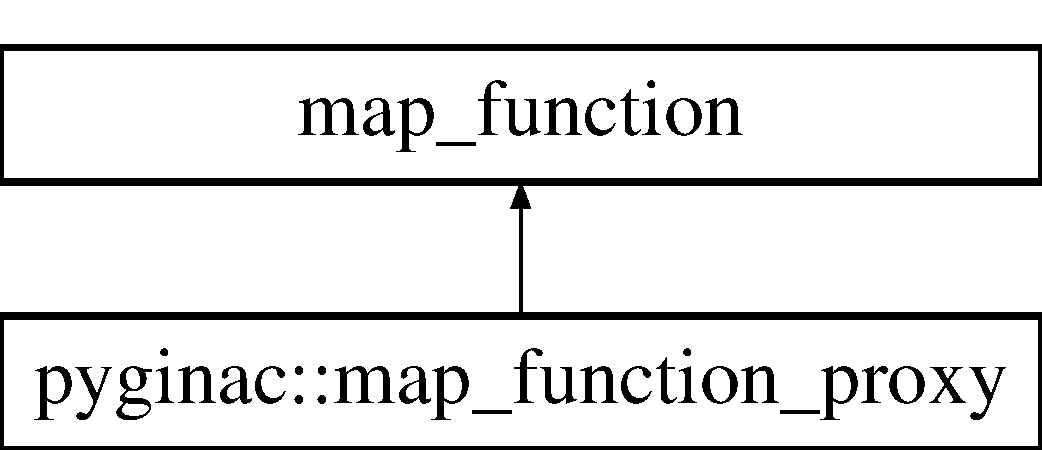
\includegraphics[height=2.000000cm]{structpyginac_1_1map__function__proxy}
\end{center}
\end{figure}
\subsection*{Public Member Functions}
\begin{DoxyCompactItemize}
\item 
\mbox{\Hypertarget{structpyginac_1_1map__function__proxy_a458fb20352a9bdfa393e45eb1b1e9b1e}\label{structpyginac_1_1map__function__proxy_a458fb20352a9bdfa393e45eb1b1e9b1e}} 
{\bfseries map\+\_\+function\+\_\+proxy} (Py\+Object $\ast$\+\_\+self)
\item 
\mbox{\Hypertarget{structpyginac_1_1map__function__proxy_aba7abc33e82832dbb5050994e4e5ca51}\label{structpyginac_1_1map__function__proxy_aba7abc33e82832dbb5050994e4e5ca51}} 
virtual Gi\+Na\+C\+::ex {\bfseries operator()} (const Gi\+Na\+C\+::ex \&arg)
\end{DoxyCompactItemize}
\subsection*{Public Attributes}
\begin{DoxyCompactItemize}
\item 
\mbox{\Hypertarget{structpyginac_1_1map__function__proxy_ad736211c6c987a875512ab1f48c5f62d}\label{structpyginac_1_1map__function__proxy_ad736211c6c987a875512ab1f48c5f62d}} 
Py\+Object $\ast$ {\bfseries self}
\end{DoxyCompactItemize}


The documentation for this struct was generated from the following file\+:\begin{DoxyCompactItemize}
\item 
/\+Users/lukehutton/\+One\+Drive -\/ University of Leeds/\+University/\+Computer Science/\+Internship/moebinv-\/gui/lib/moebinv-\/3.\+2/pyginac/src/map\+\_\+function.\+cpp\end{DoxyCompactItemize}

\hypertarget{class_ui_1_1matrix4dialog}{}\section{Ui\+:\+:matrix4dialog Class Reference}
\label{class_ui_1_1matrix4dialog}\index{Ui\+::matrix4dialog@{Ui\+::matrix4dialog}}
Inheritance diagram for Ui\+:\+:matrix4dialog\+:\begin{figure}[H]
\begin{center}
\leavevmode
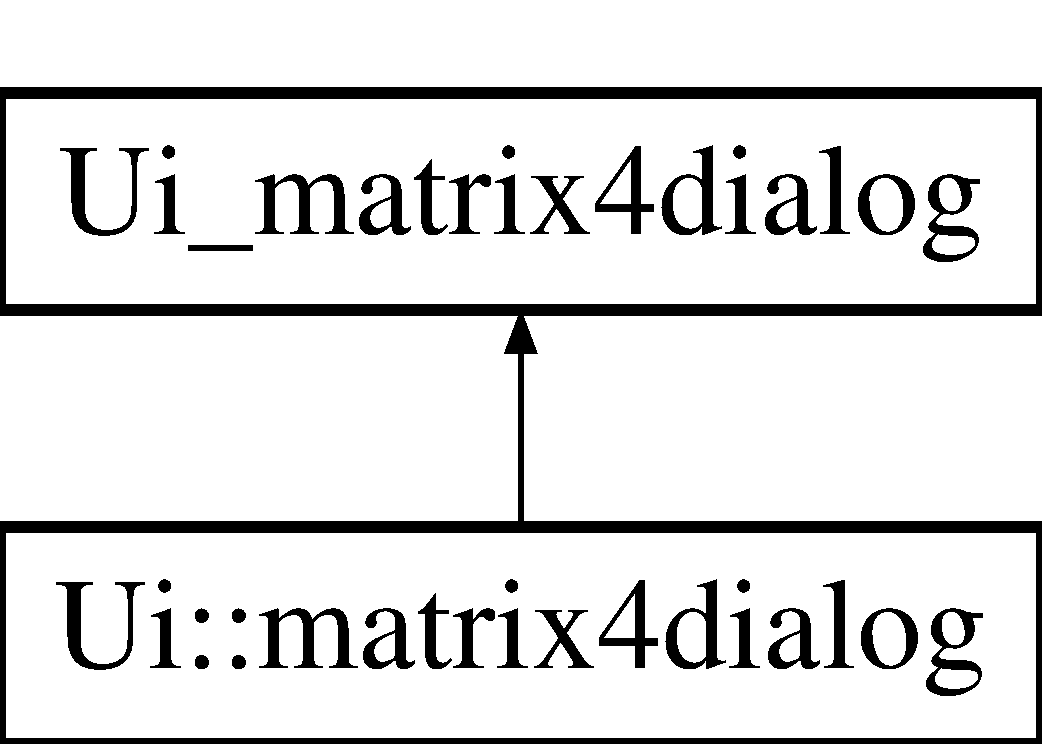
\includegraphics[height=2.000000cm]{class_ui_1_1matrix4dialog}
\end{center}
\end{figure}
\subsection*{Additional Inherited Members}


The documentation for this class was generated from the following file\+:\begin{DoxyCompactItemize}
\item 
/\+Users/lukehutton/\+One\+Drive -\/ University of Leeds/\+University/\+Computer Science/\+Internship/moebinv-\/gui/moebinv-\/gui-\/build/ui\+\_\+matrix4dialog.\+h\end{DoxyCompactItemize}

\hypertarget{classmatrix4dialog}{}\section{matrix4dialog Class Reference}
\label{classmatrix4dialog}\index{matrix4dialog@{matrix4dialog}}
Inheritance diagram for matrix4dialog\+:\begin{figure}[H]
\begin{center}
\leavevmode
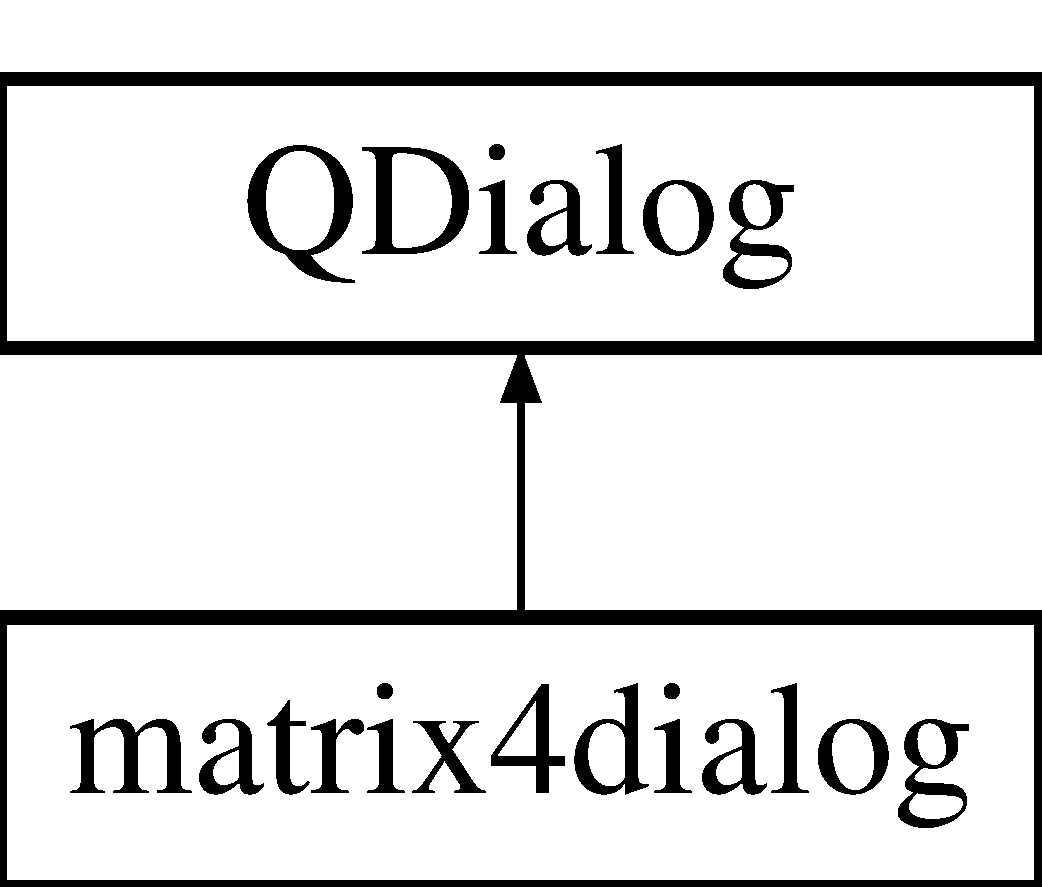
\includegraphics[height=2.000000cm]{classmatrix4dialog}
\end{center}
\end{figure}
\subsection*{Public Member Functions}
\begin{DoxyCompactItemize}
\item 
\mbox{\hyperlink{classmatrix4dialog_a5f97315156e47939f8811cce88d8e580}{matrix4dialog}} (Q\+Widget $\ast$parent=0)
\begin{DoxyCompactList}\small\item\em \mbox{\hyperlink{classmatrix4dialog_a5f97315156e47939f8811cce88d8e580}{matrix4dialog\+::matrix4dialog}} \end{DoxyCompactList}\item 
void \mbox{\hyperlink{classmatrix4dialog_a4826be428cb3f2d79905aee086cc296d}{get\+Values}} (Gi\+Na\+C\+::lst $\ast$input\+List)
\begin{DoxyCompactList}\small\item\em \mbox{\hyperlink{classmatrix4dialog_a4826be428cb3f2d79905aee086cc296d}{matrix4dialog\+::get\+Values}} \end{DoxyCompactList}\item 
\mbox{\hyperlink{classmatrix4dialog_aebc069268fc2120b95dc75338b03cb68}{$\sim$matrix4dialog}} ()
\begin{DoxyCompactList}\small\item\em \mbox{\hyperlink{classmatrix4dialog_aebc069268fc2120b95dc75338b03cb68}{matrix4dialog\+::$\sim$matrix4dialog}} \end{DoxyCompactList}\end{DoxyCompactItemize}


\subsection{Constructor \& Destructor Documentation}
\mbox{\Hypertarget{classmatrix4dialog_a5f97315156e47939f8811cce88d8e580}\label{classmatrix4dialog_a5f97315156e47939f8811cce88d8e580}} 
\index{matrix4dialog@{matrix4dialog}!matrix4dialog@{matrix4dialog}}
\index{matrix4dialog@{matrix4dialog}!matrix4dialog@{matrix4dialog}}
\subsubsection{\texorpdfstring{matrix4dialog()}{matrix4dialog()}}
{\footnotesize\ttfamily matrix4dialog\+::matrix4dialog (\begin{DoxyParamCaption}\item[{Q\+Widget $\ast$}]{parent = {\ttfamily 0} }\end{DoxyParamCaption})\hspace{0.3cm}{\ttfamily [explicit]}}



\mbox{\hyperlink{classmatrix4dialog_a5f97315156e47939f8811cce88d8e580}{matrix4dialog\+::matrix4dialog}} 


\begin{DoxyParams}{Parameters}
{\em parent} & Creates a new \mbox{\hyperlink{classmatrix4dialog}{matrix4dialog}}. Allows the user to enter 4 double values. \\
\hline
\end{DoxyParams}
\mbox{\Hypertarget{classmatrix4dialog_aebc069268fc2120b95dc75338b03cb68}\label{classmatrix4dialog_aebc069268fc2120b95dc75338b03cb68}} 
\index{matrix4dialog@{matrix4dialog}!````~matrix4dialog@{$\sim$matrix4dialog}}
\index{````~matrix4dialog@{$\sim$matrix4dialog}!matrix4dialog@{matrix4dialog}}
\subsubsection{\texorpdfstring{$\sim$matrix4dialog()}{~matrix4dialog()}}
{\footnotesize\ttfamily matrix4dialog\+::$\sim$matrix4dialog (\begin{DoxyParamCaption}{ }\end{DoxyParamCaption})}



\mbox{\hyperlink{classmatrix4dialog_aebc069268fc2120b95dc75338b03cb68}{matrix4dialog\+::$\sim$matrix4dialog}} 

Destructor for the \mbox{\hyperlink{classmatrix4dialog}{matrix4dialog}} 

\subsection{Member Function Documentation}
\mbox{\Hypertarget{classmatrix4dialog_a4826be428cb3f2d79905aee086cc296d}\label{classmatrix4dialog_a4826be428cb3f2d79905aee086cc296d}} 
\index{matrix4dialog@{matrix4dialog}!get\+Values@{get\+Values}}
\index{get\+Values@{get\+Values}!matrix4dialog@{matrix4dialog}}
\subsubsection{\texorpdfstring{get\+Values()}{getValues()}}
{\footnotesize\ttfamily void matrix4dialog\+::get\+Values (\begin{DoxyParamCaption}\item[{Gi\+Na\+C\+::lst $\ast$}]{input\+List }\end{DoxyParamCaption})}



\mbox{\hyperlink{classmatrix4dialog_a4826be428cb3f2d79905aee086cc296d}{matrix4dialog\+::get\+Values}} 


\begin{DoxyParams}{Parameters}
{\em input\+List} & Gets the values input into the dialog and appends each value to a Gi\+Na\+C\+::lst. \\
\hline
\end{DoxyParams}


The documentation for this class was generated from the following files\+:\begin{DoxyCompactItemize}
\item 
/\+Users/lukehutton/\+One\+Drive -\/ University of Leeds/\+University/\+Computer Science/\+Internship/moebinv-\/gui/include/matrix4dialog.\+h\item 
/\+Users/lukehutton/\+One\+Drive -\/ University of Leeds/\+University/\+Computer Science/\+Internship/moebinv-\/gui/src/matrix4dialog.\+cpp\end{DoxyCompactItemize}

\hypertarget{class_ui_1_1matrix8dialog}{}\section{Ui\+:\+:matrix8dialog Class Reference}
\label{class_ui_1_1matrix8dialog}\index{Ui\+::matrix8dialog@{Ui\+::matrix8dialog}}
Inheritance diagram for Ui\+:\+:matrix8dialog\+:\begin{figure}[H]
\begin{center}
\leavevmode
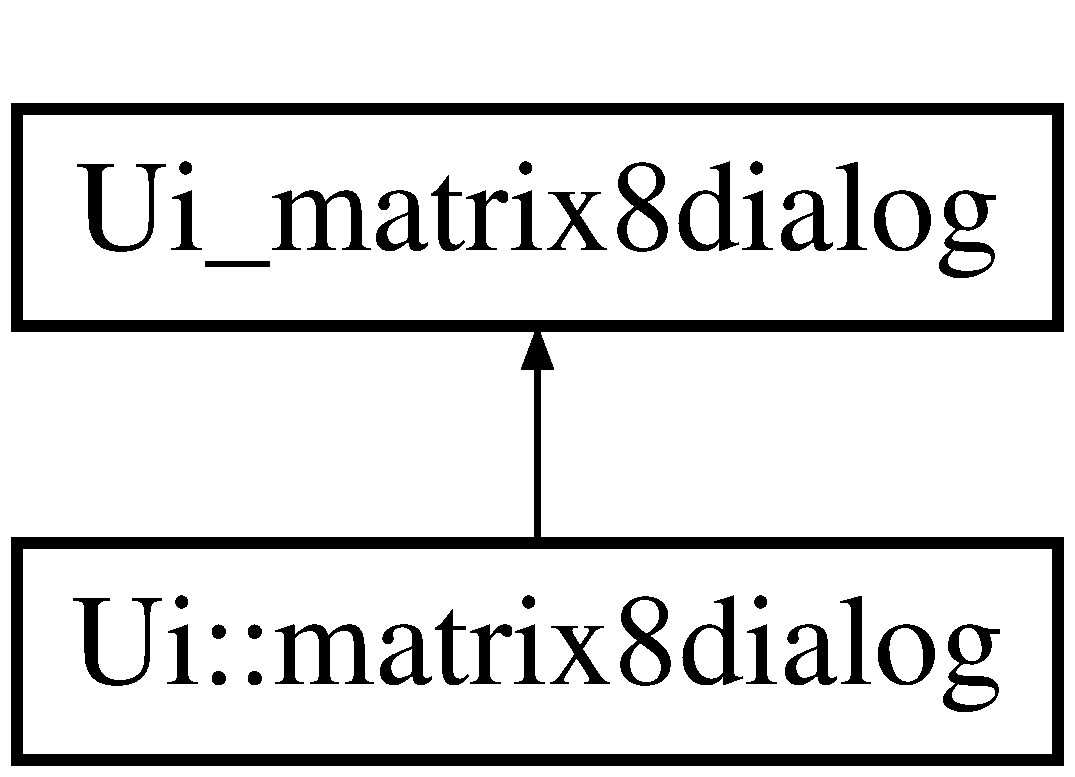
\includegraphics[height=2.000000cm]{class_ui_1_1matrix8dialog}
\end{center}
\end{figure}
\subsection*{Additional Inherited Members}


The documentation for this class was generated from the following file\+:\begin{DoxyCompactItemize}
\item 
/\+Users/lukehutton/\+One\+Drive -\/ University of Leeds/\+University/\+Computer Science/\+Internship/moebinv-\/gui/moebinv-\/gui-\/build/ui\+\_\+matrix8dialog.\+h\end{DoxyCompactItemize}

\hypertarget{classmatrix8dialog}{}\section{matrix8dialog Class Reference}
\label{classmatrix8dialog}\index{matrix8dialog@{matrix8dialog}}
Inheritance diagram for matrix8dialog\+:\begin{figure}[H]
\begin{center}
\leavevmode
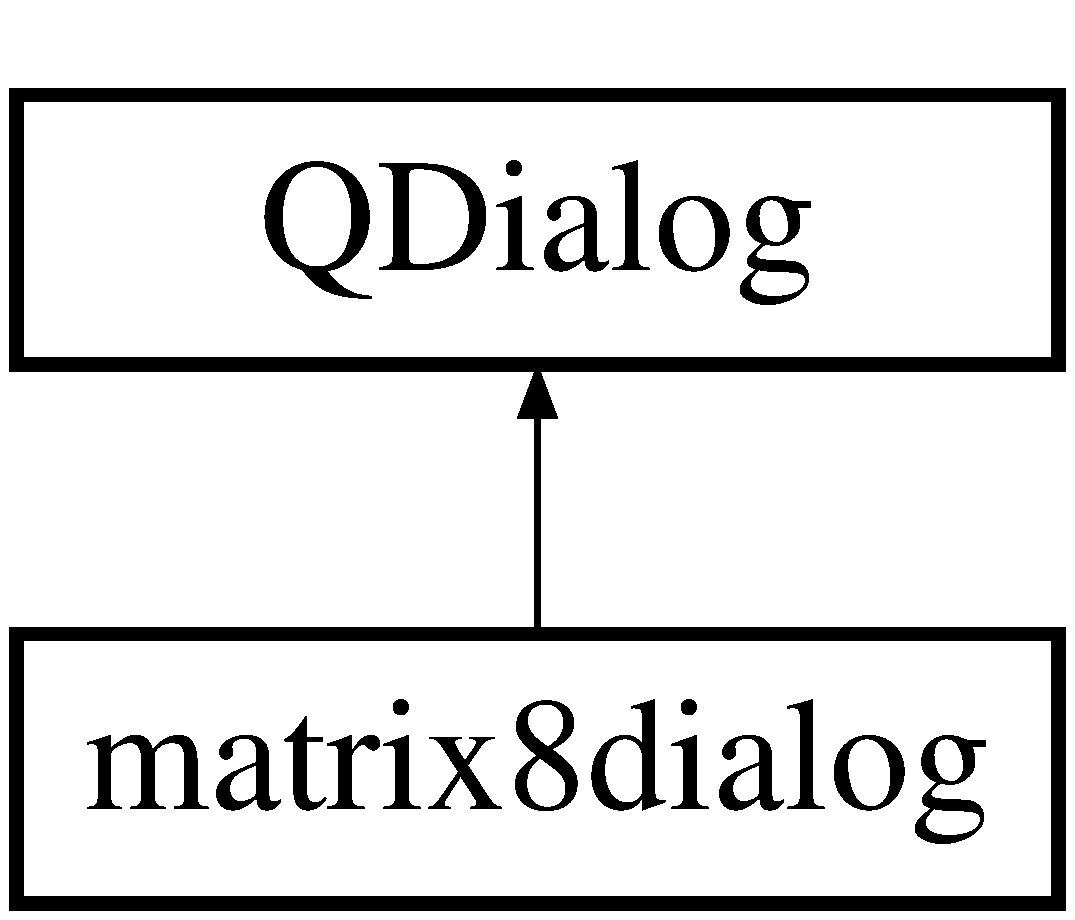
\includegraphics[height=2.000000cm]{classmatrix8dialog}
\end{center}
\end{figure}
\subsection*{Public Member Functions}
\begin{DoxyCompactItemize}
\item 
\mbox{\hyperlink{classmatrix8dialog_afcdbf5b7f9fcef31cbd030cd130d57f9}{matrix8dialog}} (Q\+Widget $\ast$parent=0)
\begin{DoxyCompactList}\small\item\em \mbox{\hyperlink{classmatrix8dialog_afcdbf5b7f9fcef31cbd030cd130d57f9}{matrix8dialog\+::matrix8dialog}} \end{DoxyCompactList}\item 
void \mbox{\hyperlink{classmatrix8dialog_a74736300c5b1a4aa0291016991c7e508}{get\+Values}} (Gi\+Na\+C\+::lst $\ast$input\+List)
\begin{DoxyCompactList}\small\item\em \mbox{\hyperlink{classmatrix8dialog_a74736300c5b1a4aa0291016991c7e508}{matrix8dialog\+::get\+Values}} \end{DoxyCompactList}\item 
\mbox{\hyperlink{classmatrix8dialog_a2caefa9ac5a7cd24f3f7713f885fe792}{$\sim$matrix8dialog}} ()
\begin{DoxyCompactList}\small\item\em \mbox{\hyperlink{classmatrix8dialog_a2caefa9ac5a7cd24f3f7713f885fe792}{matrix8dialog\+::$\sim$matrix8dialog}} \end{DoxyCompactList}\end{DoxyCompactItemize}


\subsection{Constructor \& Destructor Documentation}
\mbox{\Hypertarget{classmatrix8dialog_afcdbf5b7f9fcef31cbd030cd130d57f9}\label{classmatrix8dialog_afcdbf5b7f9fcef31cbd030cd130d57f9}} 
\index{matrix8dialog@{matrix8dialog}!matrix8dialog@{matrix8dialog}}
\index{matrix8dialog@{matrix8dialog}!matrix8dialog@{matrix8dialog}}
\subsubsection{\texorpdfstring{matrix8dialog()}{matrix8dialog()}}
{\footnotesize\ttfamily matrix8dialog\+::matrix8dialog (\begin{DoxyParamCaption}\item[{Q\+Widget $\ast$}]{parent = {\ttfamily 0} }\end{DoxyParamCaption})\hspace{0.3cm}{\ttfamily [explicit]}}



\mbox{\hyperlink{classmatrix8dialog_afcdbf5b7f9fcef31cbd030cd130d57f9}{matrix8dialog\+::matrix8dialog}} 


\begin{DoxyParams}{Parameters}
{\em parent} & Creates a new \mbox{\hyperlink{classmatrix8dialog}{matrix8dialog}}. Allows the user to enter 8 double values. \\
\hline
\end{DoxyParams}
\mbox{\Hypertarget{classmatrix8dialog_a2caefa9ac5a7cd24f3f7713f885fe792}\label{classmatrix8dialog_a2caefa9ac5a7cd24f3f7713f885fe792}} 
\index{matrix8dialog@{matrix8dialog}!````~matrix8dialog@{$\sim$matrix8dialog}}
\index{````~matrix8dialog@{$\sim$matrix8dialog}!matrix8dialog@{matrix8dialog}}
\subsubsection{\texorpdfstring{$\sim$matrix8dialog()}{~matrix8dialog()}}
{\footnotesize\ttfamily matrix8dialog\+::$\sim$matrix8dialog (\begin{DoxyParamCaption}{ }\end{DoxyParamCaption})}



\mbox{\hyperlink{classmatrix8dialog_a2caefa9ac5a7cd24f3f7713f885fe792}{matrix8dialog\+::$\sim$matrix8dialog}} 

Destructor for the \mbox{\hyperlink{classmatrix8dialog}{matrix8dialog}} 

\subsection{Member Function Documentation}
\mbox{\Hypertarget{classmatrix8dialog_a74736300c5b1a4aa0291016991c7e508}\label{classmatrix8dialog_a74736300c5b1a4aa0291016991c7e508}} 
\index{matrix8dialog@{matrix8dialog}!get\+Values@{get\+Values}}
\index{get\+Values@{get\+Values}!matrix8dialog@{matrix8dialog}}
\subsubsection{\texorpdfstring{get\+Values()}{getValues()}}
{\footnotesize\ttfamily void matrix8dialog\+::get\+Values (\begin{DoxyParamCaption}\item[{Gi\+Na\+C\+::lst $\ast$}]{input\+List }\end{DoxyParamCaption})}



\mbox{\hyperlink{classmatrix8dialog_a74736300c5b1a4aa0291016991c7e508}{matrix8dialog\+::get\+Values}} 


\begin{DoxyParams}{Parameters}
{\em input\+List} & Gets the values input into the dialog and appends each value to a Gi\+Na\+C\+::lst. \\
\hline
\end{DoxyParams}


The documentation for this class was generated from the following files\+:\begin{DoxyCompactItemize}
\item 
/\+Users/lukehutton/\+One\+Drive -\/ University of Leeds/\+University/\+Computer Science/\+Internship/moebinv-\/gui/include/matrix8dialog.\+h\item 
/\+Users/lukehutton/\+One\+Drive -\/ University of Leeds/\+University/\+Computer Science/\+Internship/moebinv-\/gui/src/matrix8dialog.\+cpp\end{DoxyCompactItemize}

\hypertarget{classmenu_rel_action}{}\section{menu\+Rel\+Action Class Reference}
\label{classmenu_rel_action}\index{menu\+Rel\+Action@{menu\+Rel\+Action}}
Inheritance diagram for menu\+Rel\+Action\+:\begin{figure}[H]
\begin{center}
\leavevmode
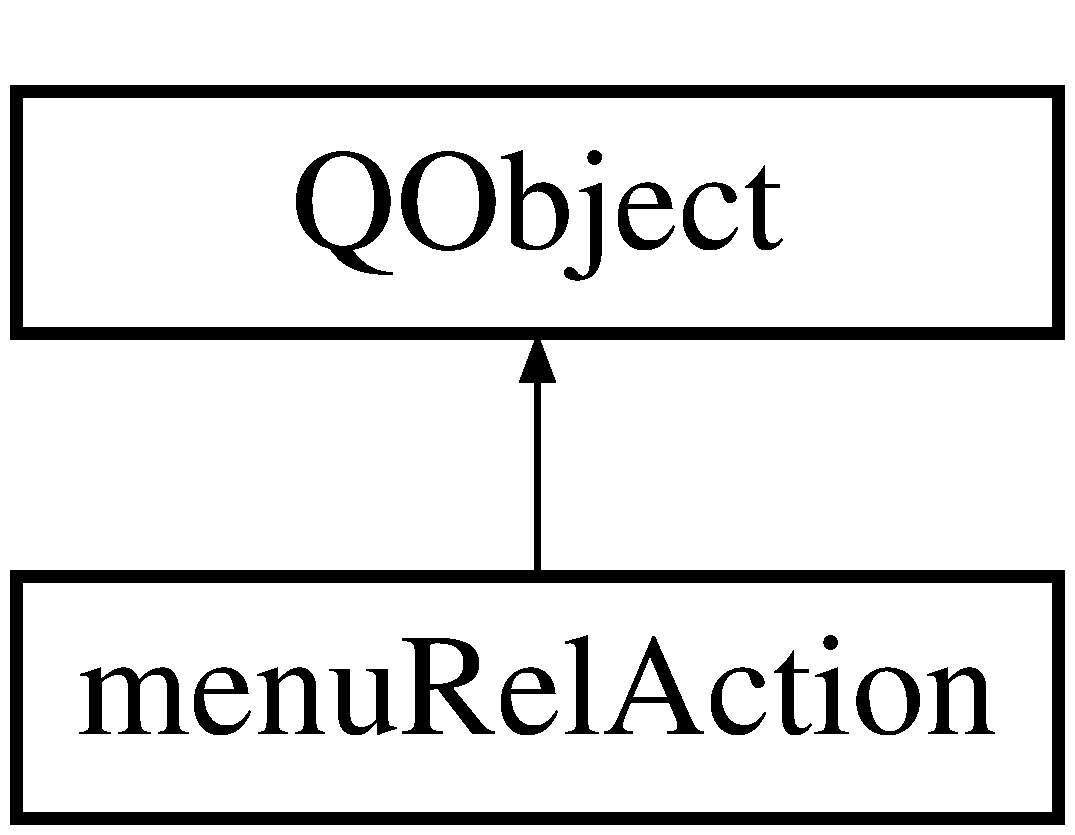
\includegraphics[height=2.000000cm]{classmenu_rel_action}
\end{center}
\end{figure}
\subsection*{Signals}
\begin{DoxyCompactItemize}
\item 
\mbox{\Hypertarget{classmenu_rel_action_a7f2a2824476be1c8e185c3b6361ad62d}\label{classmenu_rel_action_a7f2a2824476be1c8e185c3b6361ad62d}} 
void {\bfseries handle\+Relation} (const bool \&metric)
\end{DoxyCompactItemize}
\subsection*{Public Member Functions}
\begin{DoxyCompactItemize}
\item 
\mbox{\hyperlink{classmenu_rel_action_a2db14a6cd576e8cb645a0e1dcf584d4e}{menu\+Rel\+Action}} (\mbox{\hyperlink{class_moeb_inv_1_1figure}{Moeb\+Inv\+::figure}} $\ast$f, Moeb\+Inv\+::ex \mbox{\hyperlink{class_moeb_inv_1_1cycle}{cycle}}, Gi\+Na\+C\+::lst $\ast$relation\+List, Q\+String action\+Title, int params, bool checked, int rel\+Type, \mbox{\hyperlink{classmenu_rel_action_group}{menu\+Rel\+Action\+Group}} $\ast$group=nullptr)
\begin{DoxyCompactList}\small\item\em \mbox{\hyperlink{classmenu_rel_action_a2db14a6cd576e8cb645a0e1dcf584d4e}{menu\+Rel\+Action\+::menu\+Rel\+Action}} \end{DoxyCompactList}\item 
Gi\+Na\+C\+::ex \mbox{\hyperlink{classmenu_rel_action_acb80ac433c901f22dbddcff7445adf24}{get\+Cycle}} ()
\begin{DoxyCompactList}\small\item\em \mbox{\hyperlink{classmenu_rel_action_acb80ac433c901f22dbddcff7445adf24}{menu\+Rel\+Action\+::get\+Cycle}} Get the cycle assigned to this relation. \end{DoxyCompactList}\item 
int \mbox{\hyperlink{classmenu_rel_action_a1092ced0a224fdb4c8f5a0b12548a120}{get\+Rel\+Type}} ()
\begin{DoxyCompactList}\small\item\em \mbox{\hyperlink{classmenu_rel_action_a1092ced0a224fdb4c8f5a0b12548a120}{menu\+Rel\+Action\+::get\+Rel\+Type}} Get the relation type assigned to the relation. \end{DoxyCompactList}\item 
Gi\+Na\+C\+::lst \mbox{\hyperlink{classmenu_rel_action_a8ec0134231f519695901fa4d750fab4a}{get\+Input\+List}} ()
\begin{DoxyCompactList}\small\item\em \mbox{\hyperlink{classmenu_rel_action_a8ec0134231f519695901fa4d750fab4a}{menu\+Rel\+Action\+::get\+Input\+List}} gets a list of inputs based on the number of parameters required. \end{DoxyCompactList}\item 
Gi\+Na\+C\+::lst \mbox{\hyperlink{classmenu_rel_action_a8da5cc4f4063d4ea465d67b0aabc57e7}{get\+Params}} ()
\begin{DoxyCompactList}\small\item\em \mbox{\hyperlink{classmenu_rel_action_a8da5cc4f4063d4ea465d67b0aabc57e7}{menu\+Rel\+Action\+::get\+Params}} Get the parameters that have been provided to the relation. \end{DoxyCompactList}\item 
\mbox{\hyperlink{classmenu_rel_action_group}{menu\+Rel\+Action\+Group}} $\ast$ \mbox{\hyperlink{classmenu_rel_action_aca0baeed9c6a266d677dae8dfb25d65b}{get\+Group}} ()
\begin{DoxyCompactList}\small\item\em \mbox{\hyperlink{classmenu_rel_action_aca0baeed9c6a266d677dae8dfb25d65b}{menu\+Rel\+Action\+::get\+Group}} Get the group the relation has been assigned to. \end{DoxyCompactList}\item 
\mbox{\hyperlink{class_moeb_inv_1_1cycle__relation}{Moeb\+Inv\+::cycle\+\_\+relation}} \mbox{\hyperlink{classmenu_rel_action_a34deae132c511b7e34af97585df9245c}{get\+Relation}} ()
\begin{DoxyCompactList}\small\item\em \mbox{\hyperlink{classmenu_rel_action_a34deae132c511b7e34af97585df9245c}{menu\+Rel\+Action\+::get\+Relation}} Get the relation that has been assigned to the action. \end{DoxyCompactList}\item 
\mbox{\Hypertarget{classmenu_rel_action_acba36fb50f54a72a4b253957f2f50f92}\label{classmenu_rel_action_acba36fb50f54a72a4b253957f2f50f92}} 
void {\bfseries set\+Relation} ()
\item 
bool \mbox{\hyperlink{classmenu_rel_action_a5e6339dbaf4cf0dc9543afdfc5b9e15a}{has\+Relation}} ()
\begin{DoxyCompactList}\small\item\em \mbox{\hyperlink{classmenu_rel_action_a5e6339dbaf4cf0dc9543afdfc5b9e15a}{menu\+Rel\+Action\+::has\+Relation}} Check whether the action has a relation that has been assigned to it. \end{DoxyCompactList}\item 
\mbox{\Hypertarget{classmenu_rel_action_af3463f9fd28cf1ff44c672dedb89af95}\label{classmenu_rel_action_af3463f9fd28cf1ff44c672dedb89af95}} 
Q\+Action {\bfseries menu\+Entry} ()
\item 
\mbox{\Hypertarget{classmenu_rel_action_a9c40a2e1e1538829214a2a9e06896a99}\label{classmenu_rel_action_a9c40a2e1e1538829214a2a9e06896a99}} 
Q\+Action {\bfseries check\+Menu\+Entry} ()
\item 
void \mbox{\hyperlink{classmenu_rel_action_a23b63e5bdb79e12f74bd1d33a53fb6e0}{action\+Handler}} ()
\begin{DoxyCompactList}\small\item\em \mbox{\hyperlink{classmenu_rel_action_a23b63e5bdb79e12f74bd1d33a53fb6e0}{menu\+Rel\+Action\+::action\+Handler}} Handles the action. \end{DoxyCompactList}\item 
void \mbox{\hyperlink{classmenu_rel_action_adbd43b99466f9ad2cde1934e1599ae4c}{cycle\+Metric\+Action\+Handler}} ()
\begin{DoxyCompactList}\small\item\em \mbox{\hyperlink{classmenu_rel_action_adbd43b99466f9ad2cde1934e1599ae4c}{menu\+Rel\+Action\+::cycle\+Metric\+Action\+Handler}} Action handler for the cycle metric relation. \end{DoxyCompactList}\item 
\mbox{\Hypertarget{classmenu_rel_action_a1535eb0d2ad06bd4d44f3de8761841b2}\label{classmenu_rel_action_a1535eb0d2ad06bd4d44f3de8761841b2}} 
void \mbox{\hyperlink{classmenu_rel_action_a1535eb0d2ad06bd4d44f3de8761841b2}{check\+Action\+Handler}} ()
\begin{DoxyCompactList}\small\item\em \mbox{\hyperlink{classmenu_rel_action_a1535eb0d2ad06bd4d44f3de8761841b2}{menu\+Rel\+Action\+::check\+Action\+Handler}} Action handler to check the status of a relation on 2 cycles. First the user is prompted to enter another cycle key, then this function checks the status of this relation and outputs the result back to the user. \end{DoxyCompactList}\item 
\mbox{\Hypertarget{classmenu_rel_action_a8d79623cfe8711e62c6f4f28d8d4c33a}\label{classmenu_rel_action_a8d79623cfe8711e62c6f4f28d8d4c33a}} 
void \mbox{\hyperlink{classmenu_rel_action_a8d79623cfe8711e62c6f4f28d8d4c33a}{check\+Action\+Cycle\+Handler}} ()
\begin{DoxyCompactList}\small\item\em \mbox{\hyperlink{classmenu_rel_action_a8d79623cfe8711e62c6f4f28d8d4c33a}{menu\+Rel\+Action\+::check\+Action\+Cycle\+Handler}} Action handler to check the status of a relation on 2 cycles. First the user is prompted to enter another cycle key, then this function checks the status of this relation and outputs the result back to the user. \end{DoxyCompactList}\item 
\mbox{\Hypertarget{classmenu_rel_action_a157ae072f7e1622564ff68583bb73132}\label{classmenu_rel_action_a157ae072f7e1622564ff68583bb73132}} 
Q\+String {\bfseries node\+\_\+label} (Gi\+Na\+C\+::ex name)
\item 
void \mbox{\hyperlink{classmenu_rel_action_a64a27674825379ba110fb2117a572ffe}{create\+Cycle\+Relation}} (const Gi\+Na\+C\+::lst \&params, const bool \&metric)
\begin{DoxyCompactList}\small\item\em \mbox{\hyperlink{classmenu_rel_action_a64a27674825379ba110fb2117a572ffe}{menu\+Rel\+Action\+::create\+Cycle\+Relation}} creates the relevent relation based on the inputs. \end{DoxyCompactList}\item 
Q\+String \mbox{\hyperlink{classmenu_rel_action_aae6e2ce0d9d17c13d502984dda8a4a54}{check\+Cycle\+Relation}} (const Gi\+Na\+C\+::ex \&this\+Cycle, const Gi\+Na\+C\+::ex \&other\+Cycle, const bool \&metric)
\begin{DoxyCompactList}\small\item\em \mbox{\hyperlink{classmenu_rel_action_aae6e2ce0d9d17c13d502984dda8a4a54}{menu\+Rel\+Action\+::check\+Cycle\+Relation}} used to check a relation. \end{DoxyCompactList}\end{DoxyCompactItemize}
\subsection*{Public Attributes}
\begin{DoxyCompactItemize}
\item 
\mbox{\Hypertarget{classmenu_rel_action_ad9c9c61008821fcef78633ed38b42f8c}\label{classmenu_rel_action_ad9c9c61008821fcef78633ed38b42f8c}} 
Q\+Action $\ast$ {\bfseries add\+Relation}
\item 
\mbox{\Hypertarget{classmenu_rel_action_ab78b5ed63bee30881b70110161670fb5}\label{classmenu_rel_action_ab78b5ed63bee30881b70110161670fb5}} 
Q\+Action $\ast$ {\bfseries add\+Cycle\+Relation}
\item 
\mbox{\Hypertarget{classmenu_rel_action_afa273b825fbdc2d887cc6a3ecfc62265}\label{classmenu_rel_action_afa273b825fbdc2d887cc6a3ecfc62265}} 
Q\+Action $\ast$ {\bfseries check\+Relation}
\item 
\mbox{\Hypertarget{classmenu_rel_action_a7937666c8189cb7597874642917e83ec}\label{classmenu_rel_action_a7937666c8189cb7597874642917e83ec}} 
Q\+Action $\ast$ {\bfseries check\+Cycle\+Metric\+Relation}
\end{DoxyCompactItemize}


\subsection{Constructor \& Destructor Documentation}
\mbox{\Hypertarget{classmenu_rel_action_a2db14a6cd576e8cb645a0e1dcf584d4e}\label{classmenu_rel_action_a2db14a6cd576e8cb645a0e1dcf584d4e}} 
\index{menu\+Rel\+Action@{menu\+Rel\+Action}!menu\+Rel\+Action@{menu\+Rel\+Action}}
\index{menu\+Rel\+Action@{menu\+Rel\+Action}!menu\+Rel\+Action@{menu\+Rel\+Action}}
\subsubsection{\texorpdfstring{menu\+Rel\+Action()}{menuRelAction()}}
{\footnotesize\ttfamily menu\+Rel\+Action\+::menu\+Rel\+Action (\begin{DoxyParamCaption}\item[{\mbox{\hyperlink{class_moeb_inv_1_1figure}{Moeb\+Inv\+::figure}} $\ast$}]{f,  }\item[{Moeb\+Inv\+::ex}]{cycle,  }\item[{Gi\+Na\+C\+::lst $\ast$}]{relation\+List,  }\item[{Q\+String}]{action\+Title,  }\item[{int}]{params,  }\item[{bool}]{checked,  }\item[{int}]{rel\+Type,  }\item[{\mbox{\hyperlink{classmenu_rel_action_group}{menu\+Rel\+Action\+Group}} $\ast$}]{group = {\ttfamily nullptr} }\end{DoxyParamCaption})}



\mbox{\hyperlink{classmenu_rel_action_a2db14a6cd576e8cb645a0e1dcf584d4e}{menu\+Rel\+Action\+::menu\+Rel\+Action}} 


\begin{DoxyParams}{Parameters}
{\em cycle} & cycle the action is related to. \\
\hline
{\em relation\+List} & pointer to the relation list that stores curretly active relations \\
\hline
{\em action\+Title} & title of the action. \\
\hline
{\em params} & number of params the relation needs to take. \\
\hline
{\em checked} & whether or not the relation is checked when created. \\
\hline
{\em rel\+Type} & the type of relation the action represents. \\
\hline
{\em group} & the group the relation is included within.\\
\hline
\end{DoxyParams}
Create a new relation Q\+Action to be added to the context menu. 

\subsection{Member Function Documentation}
\mbox{\Hypertarget{classmenu_rel_action_a23b63e5bdb79e12f74bd1d33a53fb6e0}\label{classmenu_rel_action_a23b63e5bdb79e12f74bd1d33a53fb6e0}} 
\index{menu\+Rel\+Action@{menu\+Rel\+Action}!action\+Handler@{action\+Handler}}
\index{action\+Handler@{action\+Handler}!menu\+Rel\+Action@{menu\+Rel\+Action}}
\subsubsection{\texorpdfstring{action\+Handler()}{actionHandler()}}
{\footnotesize\ttfamily void menu\+Rel\+Action\+::action\+Handler (\begin{DoxyParamCaption}{ }\end{DoxyParamCaption})}



\mbox{\hyperlink{classmenu_rel_action_a23b63e5bdb79e12f74bd1d33a53fb6e0}{menu\+Rel\+Action\+::action\+Handler}} Handles the action. 

Checks to make sure the correct number of parameters have been provided. If so the relevent relation is built. \mbox{\Hypertarget{classmenu_rel_action_aae6e2ce0d9d17c13d502984dda8a4a54}\label{classmenu_rel_action_aae6e2ce0d9d17c13d502984dda8a4a54}} 
\index{menu\+Rel\+Action@{menu\+Rel\+Action}!check\+Cycle\+Relation@{check\+Cycle\+Relation}}
\index{check\+Cycle\+Relation@{check\+Cycle\+Relation}!menu\+Rel\+Action@{menu\+Rel\+Action}}
\subsubsection{\texorpdfstring{check\+Cycle\+Relation()}{checkCycleRelation()}}
{\footnotesize\ttfamily Q\+String menu\+Rel\+Action\+::check\+Cycle\+Relation (\begin{DoxyParamCaption}\item[{const Gi\+Na\+C\+::ex \&}]{this\+Cycle,  }\item[{const Gi\+Na\+C\+::ex \&}]{other\+Cycle,  }\item[{const bool \&}]{metric }\end{DoxyParamCaption})}



\mbox{\hyperlink{classmenu_rel_action_aae6e2ce0d9d17c13d502984dda8a4a54}{menu\+Rel\+Action\+::check\+Cycle\+Relation}} used to check a relation. 


\begin{DoxyParams}{Parameters}
{\em this\+Cycle} & the cycle this relation belongs to. \\
\hline
{\em other\+Cycle} & the other cycle entered by the user. \\
\hline
\end{DoxyParams}
\begin{DoxyReturn}{Returns}
Q\+String 
\end{DoxyReturn}
\mbox{\Hypertarget{classmenu_rel_action_a64a27674825379ba110fb2117a572ffe}\label{classmenu_rel_action_a64a27674825379ba110fb2117a572ffe}} 
\index{menu\+Rel\+Action@{menu\+Rel\+Action}!create\+Cycle\+Relation@{create\+Cycle\+Relation}}
\index{create\+Cycle\+Relation@{create\+Cycle\+Relation}!menu\+Rel\+Action@{menu\+Rel\+Action}}
\subsubsection{\texorpdfstring{create\+Cycle\+Relation()}{createCycleRelation()}}
{\footnotesize\ttfamily void menu\+Rel\+Action\+::create\+Cycle\+Relation (\begin{DoxyParamCaption}\item[{const Gi\+Na\+C\+::lst \&}]{params,  }\item[{const bool \&}]{metric }\end{DoxyParamCaption})}



\mbox{\hyperlink{classmenu_rel_action_a64a27674825379ba110fb2117a572ffe}{menu\+Rel\+Action\+::create\+Cycle\+Relation}} creates the relevent relation based on the inputs. 


\begin{DoxyParams}{Parameters}
{\em params} & Gi\+Na\+C\+::lst of the parameter entered by the user. \\
\hline
{\em metric} & true = point metric relation, false = cycle metric relation \\
\hline
\end{DoxyParams}
\mbox{\Hypertarget{classmenu_rel_action_adbd43b99466f9ad2cde1934e1599ae4c}\label{classmenu_rel_action_adbd43b99466f9ad2cde1934e1599ae4c}} 
\index{menu\+Rel\+Action@{menu\+Rel\+Action}!cycle\+Metric\+Action\+Handler@{cycle\+Metric\+Action\+Handler}}
\index{cycle\+Metric\+Action\+Handler@{cycle\+Metric\+Action\+Handler}!menu\+Rel\+Action@{menu\+Rel\+Action}}
\subsubsection{\texorpdfstring{cycle\+Metric\+Action\+Handler()}{cycleMetricActionHandler()}}
{\footnotesize\ttfamily void menu\+Rel\+Action\+::cycle\+Metric\+Action\+Handler (\begin{DoxyParamCaption}{ }\end{DoxyParamCaption})}



\mbox{\hyperlink{classmenu_rel_action_adbd43b99466f9ad2cde1934e1599ae4c}{menu\+Rel\+Action\+::cycle\+Metric\+Action\+Handler}} Action handler for the cycle metric relation. 

Checks to make sure the correct number of parameters have been provided. If so the relevent relation is built. \mbox{\Hypertarget{classmenu_rel_action_acb80ac433c901f22dbddcff7445adf24}\label{classmenu_rel_action_acb80ac433c901f22dbddcff7445adf24}} 
\index{menu\+Rel\+Action@{menu\+Rel\+Action}!get\+Cycle@{get\+Cycle}}
\index{get\+Cycle@{get\+Cycle}!menu\+Rel\+Action@{menu\+Rel\+Action}}
\subsubsection{\texorpdfstring{get\+Cycle()}{getCycle()}}
{\footnotesize\ttfamily ex menu\+Rel\+Action\+::get\+Cycle (\begin{DoxyParamCaption}{ }\end{DoxyParamCaption})}



\mbox{\hyperlink{classmenu_rel_action_acb80ac433c901f22dbddcff7445adf24}{menu\+Rel\+Action\+::get\+Cycle}} Get the cycle assigned to this relation. 

\begin{DoxyReturn}{Returns}
Gi\+Na\+C\+::ex 
\end{DoxyReturn}
\mbox{\Hypertarget{classmenu_rel_action_aca0baeed9c6a266d677dae8dfb25d65b}\label{classmenu_rel_action_aca0baeed9c6a266d677dae8dfb25d65b}} 
\index{menu\+Rel\+Action@{menu\+Rel\+Action}!get\+Group@{get\+Group}}
\index{get\+Group@{get\+Group}!menu\+Rel\+Action@{menu\+Rel\+Action}}
\subsubsection{\texorpdfstring{get\+Group()}{getGroup()}}
{\footnotesize\ttfamily \mbox{\hyperlink{classmenu_rel_action_group}{menu\+Rel\+Action\+Group}} $\ast$ menu\+Rel\+Action\+::get\+Group (\begin{DoxyParamCaption}{ }\end{DoxyParamCaption})}



\mbox{\hyperlink{classmenu_rel_action_aca0baeed9c6a266d677dae8dfb25d65b}{menu\+Rel\+Action\+::get\+Group}} Get the group the relation has been assigned to. 

\begin{DoxyReturn}{Returns}
menu\+Rel\+Action\+Group$\ast$ 
\end{DoxyReturn}
\mbox{\Hypertarget{classmenu_rel_action_a8ec0134231f519695901fa4d750fab4a}\label{classmenu_rel_action_a8ec0134231f519695901fa4d750fab4a}} 
\index{menu\+Rel\+Action@{menu\+Rel\+Action}!get\+Input\+List@{get\+Input\+List}}
\index{get\+Input\+List@{get\+Input\+List}!menu\+Rel\+Action@{menu\+Rel\+Action}}
\subsubsection{\texorpdfstring{get\+Input\+List()}{getInputList()}}
{\footnotesize\ttfamily lst menu\+Rel\+Action\+::get\+Input\+List (\begin{DoxyParamCaption}{ }\end{DoxyParamCaption})}



\mbox{\hyperlink{classmenu_rel_action_a8ec0134231f519695901fa4d750fab4a}{menu\+Rel\+Action\+::get\+Input\+List}} gets a list of inputs based on the number of parameters required. 

\begin{DoxyReturn}{Returns}
Gi\+Na\+C\+::lst 
\end{DoxyReturn}
\mbox{\Hypertarget{classmenu_rel_action_a8da5cc4f4063d4ea465d67b0aabc57e7}\label{classmenu_rel_action_a8da5cc4f4063d4ea465d67b0aabc57e7}} 
\index{menu\+Rel\+Action@{menu\+Rel\+Action}!get\+Params@{get\+Params}}
\index{get\+Params@{get\+Params}!menu\+Rel\+Action@{menu\+Rel\+Action}}
\subsubsection{\texorpdfstring{get\+Params()}{getParams()}}
{\footnotesize\ttfamily lst menu\+Rel\+Action\+::get\+Params (\begin{DoxyParamCaption}{ }\end{DoxyParamCaption})}



\mbox{\hyperlink{classmenu_rel_action_a8da5cc4f4063d4ea465d67b0aabc57e7}{menu\+Rel\+Action\+::get\+Params}} Get the parameters that have been provided to the relation. 

\begin{DoxyReturn}{Returns}
Gi\+Na\+C\+::lst 
\end{DoxyReturn}
\mbox{\Hypertarget{classmenu_rel_action_a34deae132c511b7e34af97585df9245c}\label{classmenu_rel_action_a34deae132c511b7e34af97585df9245c}} 
\index{menu\+Rel\+Action@{menu\+Rel\+Action}!get\+Relation@{get\+Relation}}
\index{get\+Relation@{get\+Relation}!menu\+Rel\+Action@{menu\+Rel\+Action}}
\subsubsection{\texorpdfstring{get\+Relation()}{getRelation()}}
{\footnotesize\ttfamily \mbox{\hyperlink{class_moeb_inv_1_1cycle__relation}{cycle\+\_\+relation}} menu\+Rel\+Action\+::get\+Relation (\begin{DoxyParamCaption}{ }\end{DoxyParamCaption})}



\mbox{\hyperlink{classmenu_rel_action_a34deae132c511b7e34af97585df9245c}{menu\+Rel\+Action\+::get\+Relation}} Get the relation that has been assigned to the action. 

\begin{DoxyReturn}{Returns}
cycle\+\_\+relation 
\end{DoxyReturn}
\mbox{\Hypertarget{classmenu_rel_action_a1092ced0a224fdb4c8f5a0b12548a120}\label{classmenu_rel_action_a1092ced0a224fdb4c8f5a0b12548a120}} 
\index{menu\+Rel\+Action@{menu\+Rel\+Action}!get\+Rel\+Type@{get\+Rel\+Type}}
\index{get\+Rel\+Type@{get\+Rel\+Type}!menu\+Rel\+Action@{menu\+Rel\+Action}}
\subsubsection{\texorpdfstring{get\+Rel\+Type()}{getRelType()}}
{\footnotesize\ttfamily int menu\+Rel\+Action\+::get\+Rel\+Type (\begin{DoxyParamCaption}{ }\end{DoxyParamCaption})}



\mbox{\hyperlink{classmenu_rel_action_a1092ced0a224fdb4c8f5a0b12548a120}{menu\+Rel\+Action\+::get\+Rel\+Type}} Get the relation type assigned to the relation. 

\begin{DoxyReturn}{Returns}
int 
\end{DoxyReturn}
\mbox{\Hypertarget{classmenu_rel_action_a5e6339dbaf4cf0dc9543afdfc5b9e15a}\label{classmenu_rel_action_a5e6339dbaf4cf0dc9543afdfc5b9e15a}} 
\index{menu\+Rel\+Action@{menu\+Rel\+Action}!has\+Relation@{has\+Relation}}
\index{has\+Relation@{has\+Relation}!menu\+Rel\+Action@{menu\+Rel\+Action}}
\subsubsection{\texorpdfstring{has\+Relation()}{hasRelation()}}
{\footnotesize\ttfamily bool menu\+Rel\+Action\+::has\+Relation (\begin{DoxyParamCaption}{ }\end{DoxyParamCaption})}



\mbox{\hyperlink{classmenu_rel_action_a5e6339dbaf4cf0dc9543afdfc5b9e15a}{menu\+Rel\+Action\+::has\+Relation}} Check whether the action has a relation that has been assigned to it. 

\begin{DoxyReturn}{Returns}
bool 
\end{DoxyReturn}


The documentation for this class was generated from the following files\+:\begin{DoxyCompactItemize}
\item 
/\+Users/lukehutton/\+One\+Drive -\/ University of Leeds/\+University/\+Computer Science/\+Internship/moebinv-\/gui/include/menurelationhandler.\+h\item 
/\+Users/lukehutton/\+One\+Drive -\/ University of Leeds/\+University/\+Computer Science/\+Internship/moebinv-\/gui/src/menurelationhandler.\+cpp\end{DoxyCompactItemize}

\hypertarget{classmenu_rel_action_group}{}\section{menu\+Rel\+Action\+Group Class Reference}
\label{classmenu_rel_action_group}\index{menu\+Rel\+Action\+Group@{menu\+Rel\+Action\+Group}}
Inheritance diagram for menu\+Rel\+Action\+Group\+:\begin{figure}[H]
\begin{center}
\leavevmode
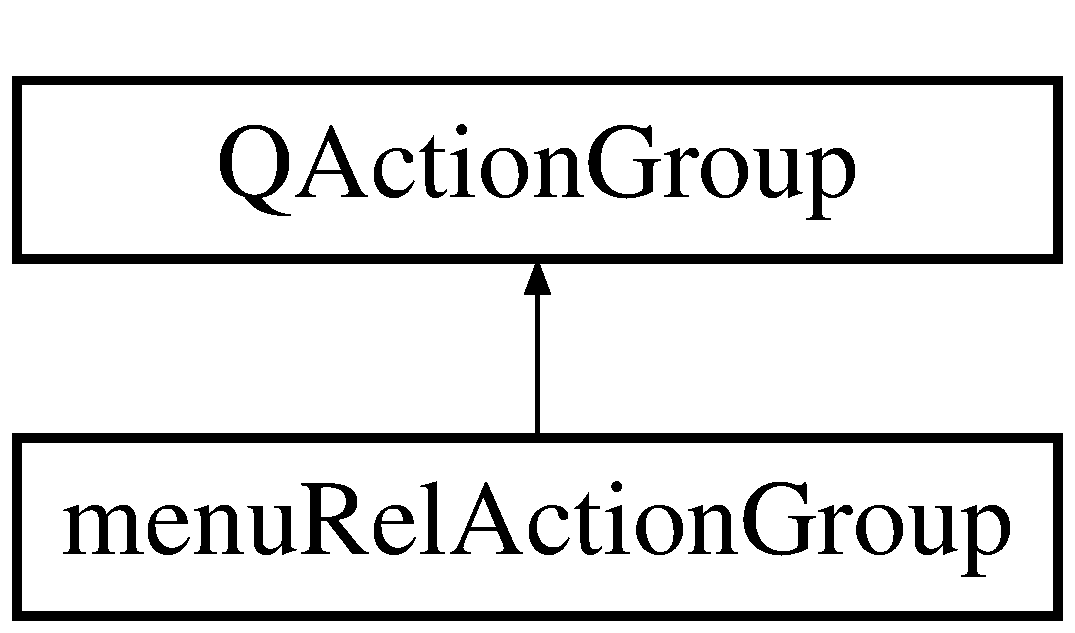
\includegraphics[height=2.000000cm]{classmenu_rel_action_group}
\end{center}
\end{figure}
\subsection*{Signals}
\begin{DoxyCompactItemize}
\item 
\mbox{\Hypertarget{classmenu_rel_action_group_a35a2675819196b79afc8f0c3701b10ed}\label{classmenu_rel_action_group_a35a2675819196b79afc8f0c3701b10ed}} 
void {\bfseries handle\+Relation} ()
\end{DoxyCompactItemize}
\subsection*{Public Member Functions}
\begin{DoxyCompactItemize}
\item 
\mbox{\hyperlink{classmenu_rel_action_group_ac43afaa3a021c3543d31e2401944938e}{menu\+Rel\+Action\+Group}} (Q\+Object $\ast$parent=nullptr)
\begin{DoxyCompactList}\small\item\em \mbox{\hyperlink{classmenu_rel_action_group_ac43afaa3a021c3543d31e2401944938e}{menu\+Rel\+Action\+Group\+::menu\+Rel\+Action\+Group}} \end{DoxyCompactList}\item 
void \mbox{\hyperlink{classmenu_rel_action_group_a7b36eb218ae45fd971c1bfca5eb465c4}{add\+Rel\+Action}} (\mbox{\hyperlink{classmenu_rel_action}{menu\+Rel\+Action}} $\ast$action)
\begin{DoxyCompactList}\small\item\em \mbox{\hyperlink{classmenu_rel_action_group_a7b36eb218ae45fd971c1bfca5eb465c4}{menu\+Rel\+Action\+Group\+::add\+Rel\+Action}} Add a new action to the group. \end{DoxyCompactList}\item 
Q\+List$<$ \mbox{\hyperlink{classmenu_rel_action}{menu\+Rel\+Action}} $\ast$ $>$ \mbox{\hyperlink{classmenu_rel_action_group_ac050bdcde34d72fc17c4fed70d2bfa6c}{get\+Rel\+Actions}} ()
\begin{DoxyCompactList}\small\item\em \mbox{\hyperlink{classmenu_rel_action_group_ac050bdcde34d72fc17c4fed70d2bfa6c}{menu\+Rel\+Action\+Group\+::get\+Rel\+Actions}} Get the actions that have been added to the group and return as a list of \mbox{\hyperlink{classmenu_rel_action}{menu\+Rel\+Action}} objects. \end{DoxyCompactList}\end{DoxyCompactItemize}


\subsection{Constructor \& Destructor Documentation}
\mbox{\Hypertarget{classmenu_rel_action_group_ac43afaa3a021c3543d31e2401944938e}\label{classmenu_rel_action_group_ac43afaa3a021c3543d31e2401944938e}} 
\index{menu\+Rel\+Action\+Group@{menu\+Rel\+Action\+Group}!menu\+Rel\+Action\+Group@{menu\+Rel\+Action\+Group}}
\index{menu\+Rel\+Action\+Group@{menu\+Rel\+Action\+Group}!menu\+Rel\+Action\+Group@{menu\+Rel\+Action\+Group}}
\subsubsection{\texorpdfstring{menu\+Rel\+Action\+Group()}{menuRelActionGroup()}}
{\footnotesize\ttfamily menu\+Rel\+Action\+Group\+::menu\+Rel\+Action\+Group (\begin{DoxyParamCaption}\item[{Q\+Object $\ast$}]{parent = {\ttfamily nullptr} }\end{DoxyParamCaption})}



\mbox{\hyperlink{classmenu_rel_action_group_ac43afaa3a021c3543d31e2401944938e}{menu\+Rel\+Action\+Group\+::menu\+Rel\+Action\+Group}} 


\begin{DoxyParams}{Parameters}
{\em parent} & Create a new relation group. Subclassed from Q\+Action\+Group \\
\hline
\end{DoxyParams}


\subsection{Member Function Documentation}
\mbox{\Hypertarget{classmenu_rel_action_group_a7b36eb218ae45fd971c1bfca5eb465c4}\label{classmenu_rel_action_group_a7b36eb218ae45fd971c1bfca5eb465c4}} 
\index{menu\+Rel\+Action\+Group@{menu\+Rel\+Action\+Group}!add\+Rel\+Action@{add\+Rel\+Action}}
\index{add\+Rel\+Action@{add\+Rel\+Action}!menu\+Rel\+Action\+Group@{menu\+Rel\+Action\+Group}}
\subsubsection{\texorpdfstring{add\+Rel\+Action()}{addRelAction()}}
{\footnotesize\ttfamily void menu\+Rel\+Action\+Group\+::add\+Rel\+Action (\begin{DoxyParamCaption}\item[{\mbox{\hyperlink{classmenu_rel_action}{menu\+Rel\+Action}} $\ast$}]{action }\end{DoxyParamCaption})}



\mbox{\hyperlink{classmenu_rel_action_group_a7b36eb218ae45fd971c1bfca5eb465c4}{menu\+Rel\+Action\+Group\+::add\+Rel\+Action}} Add a new action to the group. 


\begin{DoxyParams}{Parameters}
{\em action} & action to add to the group. \\
\hline
\end{DoxyParams}
\mbox{\Hypertarget{classmenu_rel_action_group_ac050bdcde34d72fc17c4fed70d2bfa6c}\label{classmenu_rel_action_group_ac050bdcde34d72fc17c4fed70d2bfa6c}} 
\index{menu\+Rel\+Action\+Group@{menu\+Rel\+Action\+Group}!get\+Rel\+Actions@{get\+Rel\+Actions}}
\index{get\+Rel\+Actions@{get\+Rel\+Actions}!menu\+Rel\+Action\+Group@{menu\+Rel\+Action\+Group}}
\subsubsection{\texorpdfstring{get\+Rel\+Actions()}{getRelActions()}}
{\footnotesize\ttfamily Q\+List$<$ \mbox{\hyperlink{classmenu_rel_action}{menu\+Rel\+Action}} $\ast$ $>$ menu\+Rel\+Action\+Group\+::get\+Rel\+Actions (\begin{DoxyParamCaption}{ }\end{DoxyParamCaption})}



\mbox{\hyperlink{classmenu_rel_action_group_ac050bdcde34d72fc17c4fed70d2bfa6c}{menu\+Rel\+Action\+Group\+::get\+Rel\+Actions}} Get the actions that have been added to the group and return as a list of \mbox{\hyperlink{classmenu_rel_action}{menu\+Rel\+Action}} objects. 

\begin{DoxyReturn}{Returns}
Q\+List$<$menu\+Rel\+Action $\ast$$>$ 
\end{DoxyReturn}


The documentation for this class was generated from the following files\+:\begin{DoxyCompactItemize}
\item 
/\+Users/lukehutton/\+One\+Drive -\/ University of Leeds/\+University/\+Computer Science/\+Internship/moebinv-\/gui/include/menurelationhandler.\+h\item 
/\+Users/lukehutton/\+One\+Drive -\/ University of Leeds/\+University/\+Computer Science/\+Internship/moebinv-\/gui/moebinv-\/gui-\/build/moc\+\_\+menurelationhandler.\+cpp\item 
/\+Users/lukehutton/\+One\+Drive -\/ University of Leeds/\+University/\+Computer Science/\+Internship/moebinv-\/gui/src/menurelationhandler.\+cpp\end{DoxyCompactItemize}

\hypertarget{structpyginac_1_1numeric__from__number}{}\section{pyginac\+:\+:numeric\+\_\+from\+\_\+number Struct Reference}
\label{structpyginac_1_1numeric__from__number}\index{pyginac\+::numeric\+\_\+from\+\_\+number@{pyginac\+::numeric\+\_\+from\+\_\+number}}
\subsection*{Static Public Member Functions}
\begin{DoxyCompactItemize}
\item 
\mbox{\Hypertarget{structpyginac_1_1numeric__from__number_aa13765d6a3a07e59242b8389fc7dbcab}\label{structpyginac_1_1numeric__from__number_aa13765d6a3a07e59242b8389fc7dbcab}} 
static void $\ast$ {\bfseries convertible} (Py\+Object $\ast$obj)
\item 
\mbox{\Hypertarget{structpyginac_1_1numeric__from__number_a64dbc1aa68695a8d660b02a554d626bd}\label{structpyginac_1_1numeric__from__number_a64dbc1aa68695a8d660b02a554d626bd}} 
static void {\bfseries construct} (Py\+Object $\ast$obj, boost\+::python\+::converter\+::rvalue\+\_\+from\+\_\+python\+\_\+stage1\+\_\+data $\ast$data)
\end{DoxyCompactItemize}


The documentation for this struct was generated from the following file\+:\begin{DoxyCompactItemize}
\item 
/\+Users/lukehutton/\+One\+Drive -\/ University of Leeds/\+University/\+Computer Science/\+Internship/moebinv-\/gui/lib/moebinv-\/3.\+2/pyginac/src/numeric.\+cpp\end{DoxyCompactItemize}

\hypertarget{class_moeb_inv_1_1paravector}{}\section{Moeb\+Inv\+:\+:paravector Class Reference}
\label{class_moeb_inv_1_1paravector}\index{Moeb\+Inv\+::paravector@{Moeb\+Inv\+::paravector}}
Inheritance diagram for Moeb\+Inv\+:\+:paravector\+:\begin{figure}[H]
\begin{center}
\leavevmode
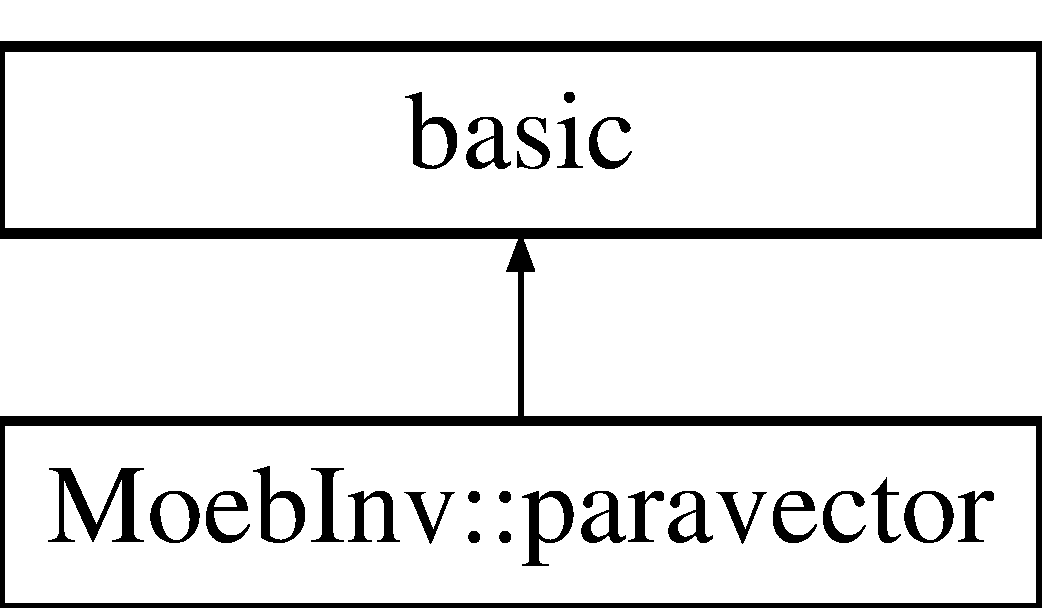
\includegraphics[height=2.000000cm]{class_moeb_inv_1_1paravector}
\end{center}
\end{figure}
\subsection*{Public Member Functions}
\begin{DoxyCompactItemize}
\item 
\mbox{\Hypertarget{class_moeb_inv_1_1paravector_a9da910ab200b81161d50a6ab40067572}\label{class_moeb_inv_1_1paravector_a9da910ab200b81161d50a6ab40067572}} 
{\bfseries paravector} (const ex \&b)
\item 
\mbox{\Hypertarget{class_moeb_inv_1_1paravector_a7d9d24c6777afead4c762c68640869aa}\label{class_moeb_inv_1_1paravector_a7d9d24c6777afead4c762c68640869aa}} 
void {\bfseries archive} (archive\+\_\+node \&n) const
\item 
\mbox{\Hypertarget{class_moeb_inv_1_1paravector_acf4bf91213a25edb147df9ecfc4ad0a8}\label{class_moeb_inv_1_1paravector_acf4bf91213a25edb147df9ecfc4ad0a8}} 
void {\bfseries read\+\_\+archive} (const archive\+\_\+node \&n, lst \&sym\+\_\+lst)
\item 
\mbox{\Hypertarget{class_moeb_inv_1_1paravector_a1cbe8eb73a9ce64fe4228173dfacd21d}\label{class_moeb_inv_1_1paravector_a1cbe8eb73a9ce64fe4228173dfacd21d}} 
return\+\_\+type\+\_\+t {\bfseries return\+\_\+type\+\_\+tinfo} () const
\item 
\mbox{\Hypertarget{class_moeb_inv_1_1paravector_a5db3f531815d5c66305ea93cae484cd8}\label{class_moeb_inv_1_1paravector_a5db3f531815d5c66305ea93cae484cd8}} 
void {\bfseries do\+\_\+print} (const print\+\_\+dflt \&c, unsigned level) const
\item 
\mbox{\Hypertarget{class_moeb_inv_1_1paravector_a324b951f813225e89ca36884309e322e}\label{class_moeb_inv_1_1paravector_a324b951f813225e89ca36884309e322e}} 
void {\bfseries do\+\_\+print\+\_\+dflt} (const print\+\_\+dflt \&c, unsigned level) const
\item 
\mbox{\Hypertarget{class_moeb_inv_1_1paravector_a78cb1eb0f441e51c389825c3f89ffa79}\label{class_moeb_inv_1_1paravector_a78cb1eb0f441e51c389825c3f89ffa79}} 
void {\bfseries do\+\_\+print\+\_\+latex} (const print\+\_\+latex \&c, unsigned level) const
\item 
\mbox{\Hypertarget{class_moeb_inv_1_1paravector_a3410467f4885f915ff8d0da7ae0564ee}\label{class_moeb_inv_1_1paravector_a3410467f4885f915ff8d0da7ae0564ee}} 
size\+\_\+t {\bfseries nops} (size\+\_\+t i) const
\item 
\mbox{\Hypertarget{class_moeb_inv_1_1paravector_a57c171c48638d93646d331f35390ddb4}\label{class_moeb_inv_1_1paravector_a57c171c48638d93646d331f35390ddb4}} 
ex {\bfseries op} (size\+\_\+t i) const
\item 
\mbox{\Hypertarget{class_moeb_inv_1_1paravector_a02cf54eb6955a808efbb1327ce272736}\label{class_moeb_inv_1_1paravector_a02cf54eb6955a808efbb1327ce272736}} 
ex \& {\bfseries let\+\_\+op} (size\+\_\+t i)
\item 
\mbox{\Hypertarget{class_moeb_inv_1_1paravector_acaf6c490368d4e7ec4f0ed50e6945f13}\label{class_moeb_inv_1_1paravector_acaf6c490368d4e7ec4f0ed50e6945f13}} 
ex {\bfseries subs} (const ex \&e, unsigned options=0) const
\item 
\mbox{\Hypertarget{class_moeb_inv_1_1paravector_a7536e454cf2e175d65b3c023c0360ec1}\label{class_moeb_inv_1_1paravector_a7536e454cf2e175d65b3c023c0360ec1}} 
ex {\bfseries subs} (const exmap \&m, unsigned options=0) const override
\item 
\mbox{\Hypertarget{class_moeb_inv_1_1paravector_abe706e5135af461a41c8ed27b2ee2a49}\label{class_moeb_inv_1_1paravector_abe706e5135af461a41c8ed27b2ee2a49}} 
ex {\bfseries eval\+\_\+indexed} (const basic \&i) const
\end{DoxyCompactItemize}
\subsection*{Protected Attributes}
\begin{DoxyCompactItemize}
\item 
\mbox{\Hypertarget{class_moeb_inv_1_1paravector_ac3ebeee2d10e76e9aeaa659a84ae6f24}\label{class_moeb_inv_1_1paravector_ac3ebeee2d10e76e9aeaa659a84ae6f24}} 
ex {\bfseries vector}
\end{DoxyCompactItemize}


The documentation for this class was generated from the following files\+:\begin{DoxyCompactItemize}
\item 
/\+Users/lukehutton/\+One\+Drive -\/ University of Leeds/\+University/\+Computer Science/\+Internship/moebinv-\/gui/lib/moebinv-\/3.\+2/include/cycle.\+h\item 
/\+Users/lukehutton/\+One\+Drive -\/ University of Leeds/\+University/\+Computer Science/\+Internship/moebinv-\/gui/lib/moebinv-\/3.\+2/src/cycle.\+cpp\end{DoxyCompactItemize}

\hypertarget{classpoint}{}\section{point Class Reference}
\label{classpoint}\index{point@{point}}


The point class.  




{\ttfamily \#include $<$point.\+h$>$}

Inheritance diagram for point\+:\begin{figure}[H]
\begin{center}
\leavevmode
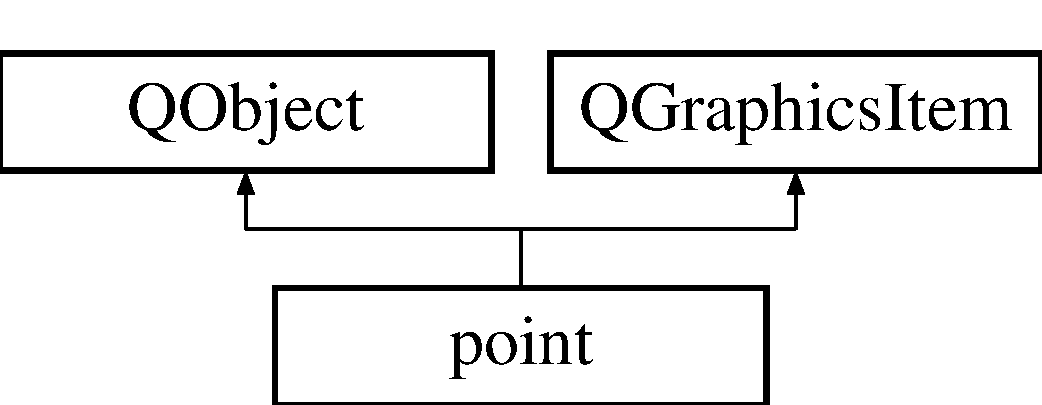
\includegraphics[height=3.000000cm]{classpoint}
\end{center}
\end{figure}
\subsection*{Public Member Functions}
\begin{DoxyCompactItemize}
\item 
\mbox{\hyperlink{classpoint_aabf8c59fffa6fb48ac1d9bcec101c3aa}{point}} (Moeb\+Inv\+::figure $\ast$f, Gi\+Na\+C\+::ex p, Q\+String l, int z)
\begin{DoxyCompactList}\small\item\em \mbox{\hyperlink{classpoint_aabf8c59fffa6fb48ac1d9bcec101c3aa}{point\+::point}} Point constructor. \end{DoxyCompactList}\item 
void \mbox{\hyperlink{classpoint_a5e75bab386500018e5d068c920ed0e66}{paint}} (Q\+Painter $\ast$p, const Q\+Style\+Option\+Graphics\+Item $\ast$, Q\+Widget $\ast$)
\begin{DoxyCompactList}\small\item\em \mbox{\hyperlink{classpoint_a5e75bab386500018e5d068c920ed0e66}{point\+::paint}} Paint the point on the scene. \end{DoxyCompactList}\item 
Q\+RectF \mbox{\hyperlink{classpoint_a91a81fc826052833e19e9d39ef3849d9}{bounding\+Rect}} () const
\begin{DoxyCompactList}\small\item\em \mbox{\hyperlink{classpoint_a91a81fc826052833e19e9d39ef3849d9}{point\+::bounding\+Rect}} Define the bounding rectangle \end{DoxyCompactList}\end{DoxyCompactItemize}
\subsection*{Additional Inherited Members}


\subsection{Detailed Description}
The point class. 

When created and added to the scene a point is displayed, given the x coordinate and y coordinates.

Inherits \mbox{\hyperlink{classgraphic_cycle}{graphic\+Cycle}}. 

\subsection{Constructor \& Destructor Documentation}
\mbox{\Hypertarget{classpoint_aabf8c59fffa6fb48ac1d9bcec101c3aa}\label{classpoint_aabf8c59fffa6fb48ac1d9bcec101c3aa}} 
\index{point@{point}!point@{point}}
\index{point@{point}!point@{point}}
\subsubsection{\texorpdfstring{point()}{point()}}
{\footnotesize\ttfamily point\+::point (\begin{DoxyParamCaption}\item[{Moeb\+Inv\+::figure $\ast$}]{f,  }\item[{Gi\+Na\+C\+::ex}]{p,  }\item[{Q\+String}]{l,  }\item[{int}]{z }\end{DoxyParamCaption})\hspace{0.3cm}{\ttfamily [explicit]}}



\mbox{\hyperlink{classpoint_aabf8c59fffa6fb48ac1d9bcec101c3aa}{point\+::point}} Point constructor. 


\begin{DoxyParams}{Parameters}
{\em f} & Moeb\+Inv figure. \\
\hline
{\em p} & Moeb\+Inv point to be drawn on the scene. \\
\hline
{\em l} & label of the point. \\
\hline
{\em z} & index in which to draw the object. \\
\hline
{\em parent} & Constructs a point on the scene.\\
\hline
\end{DoxyParams}
Inherits \textquotesingle{}\mbox{\hyperlink{classgraphic_cycle}{graphic\+Cycle}}\textquotesingle{}. 

\subsection{Member Function Documentation}
\mbox{\Hypertarget{classpoint_a91a81fc826052833e19e9d39ef3849d9}\label{classpoint_a91a81fc826052833e19e9d39ef3849d9}} 
\index{point@{point}!bounding\+Rect@{bounding\+Rect}}
\index{bounding\+Rect@{bounding\+Rect}!point@{point}}
\subsubsection{\texorpdfstring{bounding\+Rect()}{boundingRect()}}
{\footnotesize\ttfamily Q\+RectF point\+::bounding\+Rect (\begin{DoxyParamCaption}{ }\end{DoxyParamCaption}) const\hspace{0.3cm}{\ttfamily [virtual]}}



\mbox{\hyperlink{classpoint_a91a81fc826052833e19e9d39ef3849d9}{point\+::bounding\+Rect}} Define the bounding rectangle 

\begin{DoxyReturn}{Returns}
Q\+RectF
\end{DoxyReturn}
Defines the area on the scene that the object can draw on. 

Implements \mbox{\hyperlink{classgraphic_cycle}{graphic\+Cycle}}.

\mbox{\Hypertarget{classpoint_a5e75bab386500018e5d068c920ed0e66}\label{classpoint_a5e75bab386500018e5d068c920ed0e66}} 
\index{point@{point}!paint@{paint}}
\index{paint@{paint}!point@{point}}
\subsubsection{\texorpdfstring{paint()}{paint()}}
{\footnotesize\ttfamily void point\+::paint (\begin{DoxyParamCaption}\item[{Q\+Painter $\ast$}]{p,  }\item[{const Q\+Style\+Option\+Graphics\+Item $\ast$}]{,  }\item[{Q\+Widget $\ast$}]{ }\end{DoxyParamCaption})\hspace{0.3cm}{\ttfamily [virtual]}}



\mbox{\hyperlink{classpoint_a5e75bab386500018e5d068c920ed0e66}{point\+::paint}} Paint the point on the scene. 


\begin{DoxyParams}{Parameters}
{\em p} & Q\+Painter object.\\
\hline
\end{DoxyParams}
This function paints the point on the scene given various parameters (such as x, y, radius and label). The point is drawn differently dependent on the drawing metric in use. 

Implements \mbox{\hyperlink{classgraphic_cycle}{graphic\+Cycle}}.



The documentation for this class was generated from the following files\+:\begin{DoxyCompactItemize}
\item 
/\+Users/lukehutton/\+One\+Drive -\/ University of Leeds/\+University/\+Computer Science/\+Internship/moebinv-\/gui/include/point.\+h\item 
/\+Users/lukehutton/\+One\+Drive -\/ University of Leeds/\+University/\+Computer Science/\+Internship/moebinv-\/gui/src/point.\+cpp\end{DoxyCompactItemize}

\hypertarget{struct_point}{}\section{Point Struct Reference}
\label{struct_point}\index{Point@{Point}}


{\ttfamily \#include $<$vis.\+h$>$}

\subsection*{Public Attributes}
\begin{DoxyCompactItemize}
\item 
double \mbox{\hyperlink{struct_point_ab99c56589bc8ad5fa5071387110a5bc7}{x}}
\item 
double \mbox{\hyperlink{struct_point_afa38be143ae800e6ad69ce8ed4df62d8}{y}}
\item 
double \mbox{\hyperlink{struct_point_a05ba3b1dfcb19430582ae953cbbfbded}{z}}
\end{DoxyCompactItemize}


\subsection{Detailed Description}
struct containing 3 double values for use as coordinate points. 

\subsection{Member Data Documentation}
\mbox{\Hypertarget{struct_point_ab99c56589bc8ad5fa5071387110a5bc7}\label{struct_point_ab99c56589bc8ad5fa5071387110a5bc7}} 
\index{Point@{Point}!x@{x}}
\index{x@{x}!Point@{Point}}
\subsubsection{\texorpdfstring{x}{x}}
{\footnotesize\ttfamily double Point\+::x}

x coordinate of point. \mbox{\Hypertarget{struct_point_afa38be143ae800e6ad69ce8ed4df62d8}\label{struct_point_afa38be143ae800e6ad69ce8ed4df62d8}} 
\index{Point@{Point}!y@{y}}
\index{y@{y}!Point@{Point}}
\subsubsection{\texorpdfstring{y}{y}}
{\footnotesize\ttfamily double Point\+::y}

y coordinate of point. \mbox{\Hypertarget{struct_point_a05ba3b1dfcb19430582ae953cbbfbded}\label{struct_point_a05ba3b1dfcb19430582ae953cbbfbded}} 
\index{Point@{Point}!z@{z}}
\index{z@{z}!Point@{Point}}
\subsubsection{\texorpdfstring{z}{z}}
{\footnotesize\ttfamily double Point\+::z}

z coordinate of point. 

The documentation for this struct was generated from the following file\+:\begin{DoxyCompactItemize}
\item 
/\+Users/lukehutton/\+One\+Drive -\/ University of Leeds/\+University/\+Computer Science/\+Internship/moebinv-\/gui/lib/moebinv-\/3.\+2/cycle3\+D-\/visualiser/vis.\+h\end{DoxyCompactItemize}

\hypertarget{classproperties_dialog}{}\section{properties\+Dialog Class Reference}
\label{classproperties_dialog}\index{properties\+Dialog@{properties\+Dialog}}
Inheritance diagram for properties\+Dialog\+:\begin{figure}[H]
\begin{center}
\leavevmode
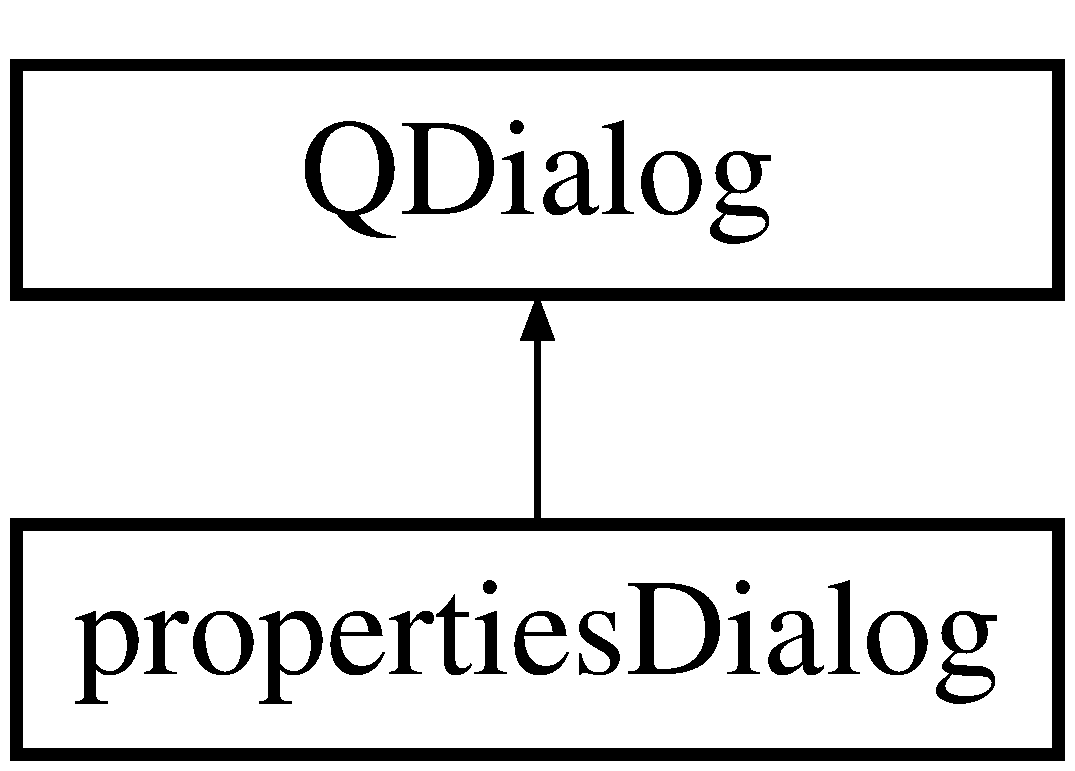
\includegraphics[height=2.000000cm]{classproperties_dialog}
\end{center}
\end{figure}
\subsection*{Signals}
\begin{DoxyCompactItemize}
\item 
\mbox{\Hypertarget{classproperties_dialog_a68bf43407ab7513191021bed8f974846}\label{classproperties_dialog_a68bf43407ab7513191021bed8f974846}} 
void {\bfseries metric\+Changed} ()
\end{DoxyCompactItemize}
\subsection*{Public Member Functions}
\begin{DoxyCompactItemize}
\item 
\mbox{\Hypertarget{classproperties_dialog_a23e5c7a841b8f1bda7adcc7d99d4da67}\label{classproperties_dialog_a23e5c7a841b8f1bda7adcc7d99d4da67}} 
{\bfseries properties\+Dialog} (Q\+Widget $\ast$parent=0)
\item 
\mbox{\Hypertarget{classproperties_dialog_a41e3286b47651d4c757bb12d34660fe6}\label{classproperties_dialog_a41e3286b47651d4c757bb12d34660fe6}} 
void {\bfseries show\+Event} (Q\+Show\+Event $\ast$event)
\item 
\mbox{\Hypertarget{classproperties_dialog_aff17b502153d16b8f19fe75bf1d06d73}\label{classproperties_dialog_aff17b502153d16b8f19fe75bf1d06d73}} 
void {\bfseries update} ()
\item 
\mbox{\Hypertarget{classproperties_dialog_ab3bdbb660ecd5514aea005e0dd59ebb5}\label{classproperties_dialog_ab3bdbb660ecd5514aea005e0dd59ebb5}} 
void \mbox{\hyperlink{classproperties_dialog_ab3bdbb660ecd5514aea005e0dd59ebb5}{load\+Values}} ()
\begin{DoxyCompactList}\small\item\em \mbox{\hyperlink{classsettings_dialog_a982beae131fefc2788432b192ec343c7}{settings\+Dialog\+::load\+Values}} This function takes the settings values that are needed for this dialog and stores them in a map where they can be edited without effecting the settings actual value. \end{DoxyCompactList}\item 
\mbox{\Hypertarget{classproperties_dialog_ab8898b89cfa3b9a310b52fbd9003dbc2}\label{classproperties_dialog_ab8898b89cfa3b9a310b52fbd9003dbc2}} 
void {\bfseries apply\+Settings} ()
\end{DoxyCompactItemize}


The documentation for this class was generated from the following files\+:\begin{DoxyCompactItemize}
\item 
/\+Users/lukehutton/\+One\+Drive -\/ University of Leeds/\+University/\+Computer Science/\+Internship/moebinv-\/gui/include/propertiesdialog.\+h\item 
/\+Users/lukehutton/\+One\+Drive -\/ University of Leeds/\+University/\+Computer Science/\+Internship/moebinv-\/gui/src/propertiesdialog.\+cpp\end{DoxyCompactItemize}

\hypertarget{class_ui_1_1properties_dialog}{}\section{Ui\+:\+:properties\+Dialog Class Reference}
\label{class_ui_1_1properties_dialog}\index{Ui\+::properties\+Dialog@{Ui\+::properties\+Dialog}}
Inheritance diagram for Ui\+:\+:properties\+Dialog\+:\begin{figure}[H]
\begin{center}
\leavevmode
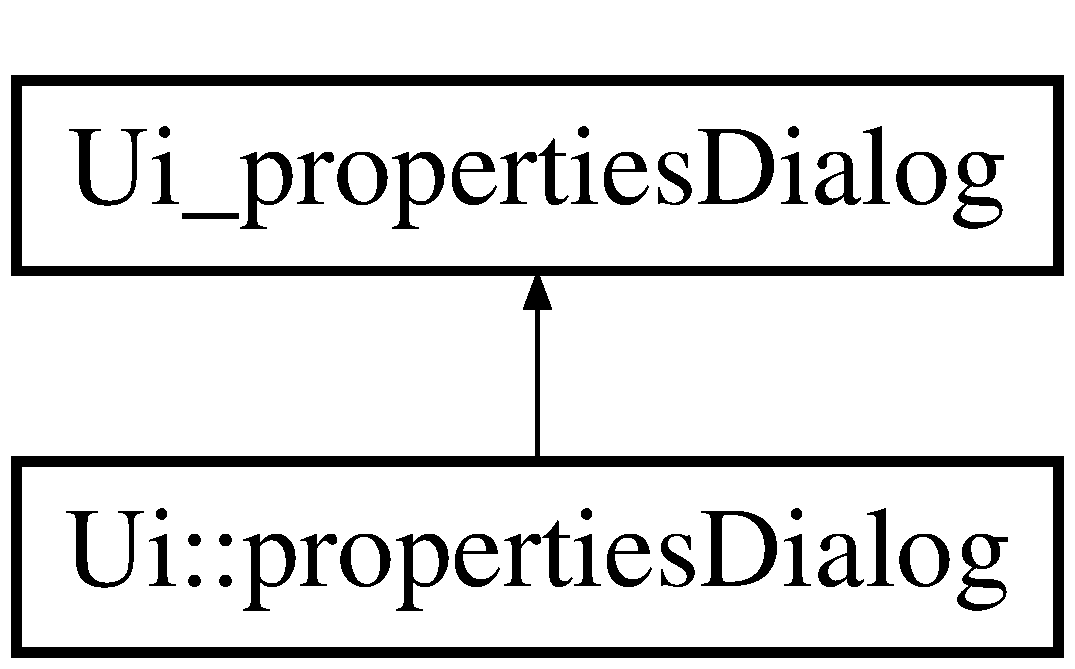
\includegraphics[height=2.000000cm]{class_ui_1_1properties_dialog}
\end{center}
\end{figure}
\subsection*{Additional Inherited Members}


The documentation for this class was generated from the following file\+:\begin{DoxyCompactItemize}
\item 
/\+Users/lukehutton/\+One\+Drive -\/ University of Leeds/\+University/\+Computer Science/\+Internship/moebinv-\/gui/moebinv-\/gui-\/build/ui\+\_\+propertiesdialog.\+h\end{DoxyCompactItemize}

\hypertarget{structqt__meta__stringdata__circle__t}{}\section{qt\+\_\+meta\+\_\+stringdata\+\_\+circle\+\_\+t Struct Reference}
\label{structqt__meta__stringdata__circle__t}\index{qt\+\_\+meta\+\_\+stringdata\+\_\+circle\+\_\+t@{qt\+\_\+meta\+\_\+stringdata\+\_\+circle\+\_\+t}}
\subsection*{Public Attributes}
\begin{DoxyCompactItemize}
\item 
\mbox{\Hypertarget{structqt__meta__stringdata__circle__t_a7930d41cb3c0ef3a8124a1d41c10946f}\label{structqt__meta__stringdata__circle__t_a7930d41cb3c0ef3a8124a1d41c10946f}} 
Q\+Byte\+Array\+Data {\bfseries data} \mbox{[}1\mbox{]}
\item 
\mbox{\Hypertarget{structqt__meta__stringdata__circle__t_ad3010a59b3cd22c250828be7413a7157}\label{structqt__meta__stringdata__circle__t_ad3010a59b3cd22c250828be7413a7157}} 
char {\bfseries stringdata0} \mbox{[}7\mbox{]}
\end{DoxyCompactItemize}


The documentation for this struct was generated from the following file\+:\begin{DoxyCompactItemize}
\item 
/\+Users/lukehutton/\+One\+Drive -\/ University of Leeds/\+University/\+Computer Science/\+Internship/moebinv-\/gui/moebinv-\/gui-\/build/moc\+\_\+circle.\+cpp\end{DoxyCompactItemize}

\hypertarget{structqt__meta__stringdata__cycle_context_menu__t}{}\section{qt\+\_\+meta\+\_\+stringdata\+\_\+cycle\+Context\+Menu\+\_\+t Struct Reference}
\label{structqt__meta__stringdata__cycle_context_menu__t}\index{qt\+\_\+meta\+\_\+stringdata\+\_\+cycle\+Context\+Menu\+\_\+t@{qt\+\_\+meta\+\_\+stringdata\+\_\+cycle\+Context\+Menu\+\_\+t}}
\subsection*{Public Attributes}
\begin{DoxyCompactItemize}
\item 
\mbox{\Hypertarget{structqt__meta__stringdata__cycle_context_menu__t_a5d7c8abf7959a17b83d045f9ad7b4c2a}\label{structqt__meta__stringdata__cycle_context_menu__t_a5d7c8abf7959a17b83d045f9ad7b4c2a}} 
Q\+Byte\+Array\+Data {\bfseries data} \mbox{[}21\mbox{]}
\item 
\mbox{\Hypertarget{structqt__meta__stringdata__cycle_context_menu__t_a51ea2171aa6b87941882cb7be4d61db8}\label{structqt__meta__stringdata__cycle_context_menu__t_a51ea2171aa6b87941882cb7be4d61db8}} 
char {\bfseries stringdata0} \mbox{[}294\mbox{]}
\end{DoxyCompactItemize}


The documentation for this struct was generated from the following file\+:\begin{DoxyCompactItemize}
\item 
/\+Users/lukehutton/\+One\+Drive -\/ University of Leeds/\+University/\+Computer Science/\+Internship/moebinv-\/gui/moebinv-\/gui-\/build/moc\+\_\+cyclecontextmenu.\+cpp\end{DoxyCompactItemize}

\hypertarget{structqt__meta__stringdata__define_cycle_dialog__t}{}\section{qt\+\_\+meta\+\_\+stringdata\+\_\+define\+Cycle\+Dialog\+\_\+t Struct Reference}
\label{structqt__meta__stringdata__define_cycle_dialog__t}\index{qt\+\_\+meta\+\_\+stringdata\+\_\+define\+Cycle\+Dialog\+\_\+t@{qt\+\_\+meta\+\_\+stringdata\+\_\+define\+Cycle\+Dialog\+\_\+t}}
\subsection*{Public Attributes}
\begin{DoxyCompactItemize}
\item 
\mbox{\Hypertarget{structqt__meta__stringdata__define_cycle_dialog__t_a5f5ff34ca5ca0e327d7051d2ce9d52d5}\label{structqt__meta__stringdata__define_cycle_dialog__t_a5f5ff34ca5ca0e327d7051d2ce9d52d5}} 
Q\+Byte\+Array\+Data {\bfseries data} \mbox{[}1\mbox{]}
\item 
\mbox{\Hypertarget{structqt__meta__stringdata__define_cycle_dialog__t_a6c71a93ad424fda6c7d2839ff9f1026f}\label{structqt__meta__stringdata__define_cycle_dialog__t_a6c71a93ad424fda6c7d2839ff9f1026f}} 
char {\bfseries stringdata0} \mbox{[}18\mbox{]}
\end{DoxyCompactItemize}


The documentation for this struct was generated from the following file\+:\begin{DoxyCompactItemize}
\item 
/\+Users/lukehutton/\+One\+Drive -\/ University of Leeds/\+University/\+Computer Science/\+Internship/moebinv-\/gui/moebinv-\/gui-\/build/moc\+\_\+definecycledialog.\+cpp\end{DoxyCompactItemize}

\hypertarget{structqt__meta__stringdata__dock_widget__t}{}\section{qt\+\_\+meta\+\_\+stringdata\+\_\+dock\+Widget\+\_\+t Struct Reference}
\label{structqt__meta__stringdata__dock_widget__t}\index{qt\+\_\+meta\+\_\+stringdata\+\_\+dock\+Widget\+\_\+t@{qt\+\_\+meta\+\_\+stringdata\+\_\+dock\+Widget\+\_\+t}}
\subsection*{Public Attributes}
\begin{DoxyCompactItemize}
\item 
\mbox{\Hypertarget{structqt__meta__stringdata__dock_widget__t_a118c54d315eed59d78416e5e4145068d}\label{structqt__meta__stringdata__dock_widget__t_a118c54d315eed59d78416e5e4145068d}} 
Q\+Byte\+Array\+Data {\bfseries data} \mbox{[}4\mbox{]}
\item 
\mbox{\Hypertarget{structqt__meta__stringdata__dock_widget__t_a1b94e2371992a973536e35688d5f62ee}\label{structqt__meta__stringdata__dock_widget__t_a1b94e2371992a973536e35688d5f62ee}} 
char {\bfseries stringdata0} \mbox{[}57\mbox{]}
\end{DoxyCompactItemize}


The documentation for this struct was generated from the following file\+:\begin{DoxyCompactItemize}
\item 
/\+Users/lukehutton/\+One\+Drive -\/ University of Leeds/\+University/\+Computer Science/\+Internship/moebinv-\/gui/moebinv-\/gui-\/build/moc\+\_\+dockwidget.\+cpp\end{DoxyCompactItemize}

\hypertarget{structqt__meta__stringdata__figure_undo_command__t}{}\section{qt\+\_\+meta\+\_\+stringdata\+\_\+figure\+Undo\+Command\+\_\+t Struct Reference}
\label{structqt__meta__stringdata__figure_undo_command__t}\index{qt\+\_\+meta\+\_\+stringdata\+\_\+figure\+Undo\+Command\+\_\+t@{qt\+\_\+meta\+\_\+stringdata\+\_\+figure\+Undo\+Command\+\_\+t}}
\subsection*{Public Attributes}
\begin{DoxyCompactItemize}
\item 
\mbox{\Hypertarget{structqt__meta__stringdata__figure_undo_command__t_ab65b436adbc0fe0249f9c76e107684a6}\label{structqt__meta__stringdata__figure_undo_command__t_ab65b436adbc0fe0249f9c76e107684a6}} 
Q\+Byte\+Array\+Data {\bfseries data} \mbox{[}5\mbox{]}
\item 
\mbox{\Hypertarget{structqt__meta__stringdata__figure_undo_command__t_ad459b353f01ec3be0cc8e2aca335b6c2}\label{structqt__meta__stringdata__figure_undo_command__t_ad459b353f01ec3be0cc8e2aca335b6c2}} 
char {\bfseries stringdata0} \mbox{[}66\mbox{]}
\end{DoxyCompactItemize}


The documentation for this struct was generated from the following file\+:\begin{DoxyCompactItemize}
\item 
/\+Users/lukehutton/\+One\+Drive -\/ University of Leeds/\+University/\+Computer Science/\+Internship/moebinv-\/gui/moebinv-\/gui-\/build/moc\+\_\+figureundocommand.\+cpp\end{DoxyCompactItemize}

\hypertarget{structqt__meta__stringdata__graphic_cycle__t}{}\section{qt\+\_\+meta\+\_\+stringdata\+\_\+graphic\+Cycle\+\_\+t Struct Reference}
\label{structqt__meta__stringdata__graphic_cycle__t}\index{qt\+\_\+meta\+\_\+stringdata\+\_\+graphic\+Cycle\+\_\+t@{qt\+\_\+meta\+\_\+stringdata\+\_\+graphic\+Cycle\+\_\+t}}
\subsection*{Public Attributes}
\begin{DoxyCompactItemize}
\item 
\mbox{\Hypertarget{structqt__meta__stringdata__graphic_cycle__t_a7d6ccfa54b966f7d6d259bdf378b3c62}\label{structqt__meta__stringdata__graphic_cycle__t_a7d6ccfa54b966f7d6d259bdf378b3c62}} 
Q\+Byte\+Array\+Data {\bfseries data} \mbox{[}20\mbox{]}
\item 
\mbox{\Hypertarget{structqt__meta__stringdata__graphic_cycle__t_a2d7f26c529a28c5e40d5a0d1522668b0}\label{structqt__meta__stringdata__graphic_cycle__t_a2d7f26c529a28c5e40d5a0d1522668b0}} 
char {\bfseries stringdata0} \mbox{[}228\mbox{]}
\end{DoxyCompactItemize}


The documentation for this struct was generated from the following file\+:\begin{DoxyCompactItemize}
\item 
/\+Users/lukehutton/\+One\+Drive -\/ University of Leeds/\+University/\+Computer Science/\+Internship/moebinv-\/gui/moebinv-\/gui-\/build/moc\+\_\+graphiccycle.\+cpp\end{DoxyCompactItemize}

\hypertarget{structqt__meta__stringdata__graphics_scene__t}{}\section{qt\+\_\+meta\+\_\+stringdata\+\_\+graphics\+Scene\+\_\+t Struct Reference}
\label{structqt__meta__stringdata__graphics_scene__t}\index{qt\+\_\+meta\+\_\+stringdata\+\_\+graphics\+Scene\+\_\+t@{qt\+\_\+meta\+\_\+stringdata\+\_\+graphics\+Scene\+\_\+t}}
\subsection*{Public Attributes}
\begin{DoxyCompactItemize}
\item 
\mbox{\Hypertarget{structqt__meta__stringdata__graphics_scene__t_a9cc8896a17a0667e790b40b5111c70aa}\label{structqt__meta__stringdata__graphics_scene__t_a9cc8896a17a0667e790b40b5111c70aa}} 
Q\+Byte\+Array\+Data {\bfseries data} \mbox{[}7\mbox{]}
\item 
\mbox{\Hypertarget{structqt__meta__stringdata__graphics_scene__t_a192f9146e5f62ea8345ecbfbc9909e8b}\label{structqt__meta__stringdata__graphics_scene__t_a192f9146e5f62ea8345ecbfbc9909e8b}} 
char {\bfseries stringdata0} \mbox{[}89\mbox{]}
\end{DoxyCompactItemize}


The documentation for this struct was generated from the following file\+:\begin{DoxyCompactItemize}
\item 
/\+Users/lukehutton/\+One\+Drive -\/ University of Leeds/\+University/\+Computer Science/\+Internship/moebinv-\/gui/moebinv-\/gui-\/build/moc\+\_\+scene.\+cpp\end{DoxyCompactItemize}

\hypertarget{structqt__meta__stringdata__help_browser__t}{}\section{qt\+\_\+meta\+\_\+stringdata\+\_\+help\+Browser\+\_\+t Struct Reference}
\label{structqt__meta__stringdata__help_browser__t}\index{qt\+\_\+meta\+\_\+stringdata\+\_\+help\+Browser\+\_\+t@{qt\+\_\+meta\+\_\+stringdata\+\_\+help\+Browser\+\_\+t}}
\subsection*{Public Attributes}
\begin{DoxyCompactItemize}
\item 
\mbox{\Hypertarget{structqt__meta__stringdata__help_browser__t_a3cd7902717b8d64da130c710bb6178a0}\label{structqt__meta__stringdata__help_browser__t_a3cd7902717b8d64da130c710bb6178a0}} 
Q\+Byte\+Array\+Data {\bfseries data} \mbox{[}1\mbox{]}
\item 
\mbox{\Hypertarget{structqt__meta__stringdata__help_browser__t_a79c6e92bd6dcec160a129977b9e80f9f}\label{structqt__meta__stringdata__help_browser__t_a79c6e92bd6dcec160a129977b9e80f9f}} 
char {\bfseries stringdata0} \mbox{[}12\mbox{]}
\end{DoxyCompactItemize}


The documentation for this struct was generated from the following file\+:\begin{DoxyCompactItemize}
\item 
/\+Users/lukehutton/\+One\+Drive -\/ University of Leeds/\+University/\+Computer Science/\+Internship/moebinv-\/gui/moebinv-\/gui-\/build/moc\+\_\+helpdialog.\+cpp\end{DoxyCompactItemize}

\hypertarget{structqt__meta__stringdata__help_dialog__t}{}\section{qt\+\_\+meta\+\_\+stringdata\+\_\+help\+Dialog\+\_\+t Struct Reference}
\label{structqt__meta__stringdata__help_dialog__t}\index{qt\+\_\+meta\+\_\+stringdata\+\_\+help\+Dialog\+\_\+t@{qt\+\_\+meta\+\_\+stringdata\+\_\+help\+Dialog\+\_\+t}}
\subsection*{Public Attributes}
\begin{DoxyCompactItemize}
\item 
\mbox{\Hypertarget{structqt__meta__stringdata__help_dialog__t_a3e6a8b85a92334ef4a1f5ef5d4ff65d9}\label{structqt__meta__stringdata__help_dialog__t_a3e6a8b85a92334ef4a1f5ef5d4ff65d9}} 
Q\+Byte\+Array\+Data {\bfseries data} \mbox{[}1\mbox{]}
\item 
\mbox{\Hypertarget{structqt__meta__stringdata__help_dialog__t_ae8fbd8a9b4ed0a5843c3fbd6410e0265}\label{structqt__meta__stringdata__help_dialog__t_ae8fbd8a9b4ed0a5843c3fbd6410e0265}} 
char {\bfseries stringdata0} \mbox{[}11\mbox{]}
\end{DoxyCompactItemize}


The documentation for this struct was generated from the following file\+:\begin{DoxyCompactItemize}
\item 
/\+Users/lukehutton/\+One\+Drive -\/ University of Leeds/\+University/\+Computer Science/\+Internship/moebinv-\/gui/moebinv-\/gui-\/build/moc\+\_\+helpdialog.\+cpp\end{DoxyCompactItemize}

\hypertarget{structqt__meta__stringdata__line__t}{}\section{qt\+\_\+meta\+\_\+stringdata\+\_\+line\+\_\+t Struct Reference}
\label{structqt__meta__stringdata__line__t}\index{qt\+\_\+meta\+\_\+stringdata\+\_\+line\+\_\+t@{qt\+\_\+meta\+\_\+stringdata\+\_\+line\+\_\+t}}
\subsection*{Public Attributes}
\begin{DoxyCompactItemize}
\item 
\mbox{\Hypertarget{structqt__meta__stringdata__line__t_a376e9f05a08dbff18309be70ba87c807}\label{structqt__meta__stringdata__line__t_a376e9f05a08dbff18309be70ba87c807}} 
Q\+Byte\+Array\+Data {\bfseries data} \mbox{[}1\mbox{]}
\item 
\mbox{\Hypertarget{structqt__meta__stringdata__line__t_aafcc21a193589e9460b20da78a228294}\label{structqt__meta__stringdata__line__t_aafcc21a193589e9460b20da78a228294}} 
char {\bfseries stringdata0} \mbox{[}5\mbox{]}
\end{DoxyCompactItemize}


The documentation for this struct was generated from the following file\+:\begin{DoxyCompactItemize}
\item 
/\+Users/lukehutton/\+One\+Drive -\/ University of Leeds/\+University/\+Computer Science/\+Internship/moebinv-\/gui/moebinv-\/gui-\/build/moc\+\_\+line.\+cpp\end{DoxyCompactItemize}

\hypertarget{structqt__meta__stringdata___main_window__t}{}\section{qt\+\_\+meta\+\_\+stringdata\+\_\+\+Main\+Window\+\_\+t Struct Reference}
\label{structqt__meta__stringdata___main_window__t}\index{qt\+\_\+meta\+\_\+stringdata\+\_\+\+Main\+Window\+\_\+t@{qt\+\_\+meta\+\_\+stringdata\+\_\+\+Main\+Window\+\_\+t}}
\subsection*{Public Attributes}
\begin{DoxyCompactItemize}
\item 
\mbox{\Hypertarget{structqt__meta__stringdata___main_window__t_af3388f2daac6273573d6d972ed5fcf91}\label{structqt__meta__stringdata___main_window__t_af3388f2daac6273573d6d972ed5fcf91}} 
Q\+Byte\+Array\+Data {\bfseries data} \mbox{[}57\mbox{]}
\item 
\mbox{\Hypertarget{structqt__meta__stringdata___main_window__t_ac30547ed7180a962035f829b57b4194f}\label{structqt__meta__stringdata___main_window__t_ac30547ed7180a962035f829b57b4194f}} 
char {\bfseries stringdata0} \mbox{[}1292\mbox{]}
\end{DoxyCompactItemize}


The documentation for this struct was generated from the following file\+:\begin{DoxyCompactItemize}
\item 
/\+Users/lukehutton/\+One\+Drive -\/ University of Leeds/\+University/\+Computer Science/\+Internship/moebinv-\/gui/moebinv-\/gui-\/build/moc\+\_\+mainwindow.\+cpp\end{DoxyCompactItemize}

\hypertarget{structqt__meta__stringdata__matrix4dialog__t}{}\section{qt\+\_\+meta\+\_\+stringdata\+\_\+matrix4dialog\+\_\+t Struct Reference}
\label{structqt__meta__stringdata__matrix4dialog__t}\index{qt\+\_\+meta\+\_\+stringdata\+\_\+matrix4dialog\+\_\+t@{qt\+\_\+meta\+\_\+stringdata\+\_\+matrix4dialog\+\_\+t}}
\subsection*{Public Attributes}
\begin{DoxyCompactItemize}
\item 
\mbox{\Hypertarget{structqt__meta__stringdata__matrix4dialog__t_a24c7d203a03bf49c7852e08c8583b12b}\label{structqt__meta__stringdata__matrix4dialog__t_a24c7d203a03bf49c7852e08c8583b12b}} 
Q\+Byte\+Array\+Data {\bfseries data} \mbox{[}1\mbox{]}
\item 
\mbox{\Hypertarget{structqt__meta__stringdata__matrix4dialog__t_a5509d1e4a8dcb461cb64d3d4c6a0f14f}\label{structqt__meta__stringdata__matrix4dialog__t_a5509d1e4a8dcb461cb64d3d4c6a0f14f}} 
char {\bfseries stringdata0} \mbox{[}14\mbox{]}
\end{DoxyCompactItemize}


The documentation for this struct was generated from the following file\+:\begin{DoxyCompactItemize}
\item 
/\+Users/lukehutton/\+One\+Drive -\/ University of Leeds/\+University/\+Computer Science/\+Internship/moebinv-\/gui/moebinv-\/gui-\/build/moc\+\_\+matrix4dialog.\+cpp\end{DoxyCompactItemize}

\hypertarget{structqt__meta__stringdata__matrix8dialog__t}{}\section{qt\+\_\+meta\+\_\+stringdata\+\_\+matrix8dialog\+\_\+t Struct Reference}
\label{structqt__meta__stringdata__matrix8dialog__t}\index{qt\+\_\+meta\+\_\+stringdata\+\_\+matrix8dialog\+\_\+t@{qt\+\_\+meta\+\_\+stringdata\+\_\+matrix8dialog\+\_\+t}}
\subsection*{Public Attributes}
\begin{DoxyCompactItemize}
\item 
\mbox{\Hypertarget{structqt__meta__stringdata__matrix8dialog__t_a9d7af3bd2bc8e32d83f86bc8f2f6fcd5}\label{structqt__meta__stringdata__matrix8dialog__t_a9d7af3bd2bc8e32d83f86bc8f2f6fcd5}} 
Q\+Byte\+Array\+Data {\bfseries data} \mbox{[}1\mbox{]}
\item 
\mbox{\Hypertarget{structqt__meta__stringdata__matrix8dialog__t_a830bc0f3c0e2785540c9fbcabea43849}\label{structqt__meta__stringdata__matrix8dialog__t_a830bc0f3c0e2785540c9fbcabea43849}} 
char {\bfseries stringdata0} \mbox{[}14\mbox{]}
\end{DoxyCompactItemize}


The documentation for this struct was generated from the following file\+:\begin{DoxyCompactItemize}
\item 
/\+Users/lukehutton/\+One\+Drive -\/ University of Leeds/\+University/\+Computer Science/\+Internship/moebinv-\/gui/moebinv-\/gui-\/build/moc\+\_\+matrix8dialog.\+cpp\end{DoxyCompactItemize}

\hypertarget{structqt__meta__stringdata__menu_rel_action__t}{}\section{qt\+\_\+meta\+\_\+stringdata\+\_\+menu\+Rel\+Action\+\_\+t Struct Reference}
\label{structqt__meta__stringdata__menu_rel_action__t}\index{qt\+\_\+meta\+\_\+stringdata\+\_\+menu\+Rel\+Action\+\_\+t@{qt\+\_\+meta\+\_\+stringdata\+\_\+menu\+Rel\+Action\+\_\+t}}
\subsection*{Public Attributes}
\begin{DoxyCompactItemize}
\item 
\mbox{\Hypertarget{structqt__meta__stringdata__menu_rel_action__t_a7b40c8a52e37a5c28251d7e999eafeaa}\label{structqt__meta__stringdata__menu_rel_action__t_a7b40c8a52e37a5c28251d7e999eafeaa}} 
Q\+Byte\+Array\+Data {\bfseries data} \mbox{[}4\mbox{]}
\item 
\mbox{\Hypertarget{structqt__meta__stringdata__menu_rel_action__t_aad12ee0e27fa96033425cf66079ba224}\label{structqt__meta__stringdata__menu_rel_action__t_aad12ee0e27fa96033425cf66079ba224}} 
char {\bfseries stringdata0} \mbox{[}37\mbox{]}
\end{DoxyCompactItemize}


The documentation for this struct was generated from the following file\+:\begin{DoxyCompactItemize}
\item 
/\+Users/lukehutton/\+One\+Drive -\/ University of Leeds/\+University/\+Computer Science/\+Internship/moebinv-\/gui/moebinv-\/gui-\/build/moc\+\_\+menurelationhandler.\+cpp\end{DoxyCompactItemize}

\hypertarget{structqt__meta__stringdata__menu_rel_action_group__t}{}\section{qt\+\_\+meta\+\_\+stringdata\+\_\+menu\+Rel\+Action\+Group\+\_\+t Struct Reference}
\label{structqt__meta__stringdata__menu_rel_action_group__t}\index{qt\+\_\+meta\+\_\+stringdata\+\_\+menu\+Rel\+Action\+Group\+\_\+t@{qt\+\_\+meta\+\_\+stringdata\+\_\+menu\+Rel\+Action\+Group\+\_\+t}}
\subsection*{Public Attributes}
\begin{DoxyCompactItemize}
\item 
\mbox{\Hypertarget{structqt__meta__stringdata__menu_rel_action_group__t_ae7569401cbdb8cde6886a1120ca52cff}\label{structqt__meta__stringdata__menu_rel_action_group__t_ae7569401cbdb8cde6886a1120ca52cff}} 
Q\+Byte\+Array\+Data {\bfseries data} \mbox{[}3\mbox{]}
\item 
\mbox{\Hypertarget{structqt__meta__stringdata__menu_rel_action_group__t_a16e48c6d600da8cd939d1fab23ece3ab}\label{structqt__meta__stringdata__menu_rel_action_group__t_a16e48c6d600da8cd939d1fab23ece3ab}} 
char {\bfseries stringdata0} \mbox{[}35\mbox{]}
\end{DoxyCompactItemize}


The documentation for this struct was generated from the following file\+:\begin{DoxyCompactItemize}
\item 
/\+Users/lukehutton/\+One\+Drive -\/ University of Leeds/\+University/\+Computer Science/\+Internship/moebinv-\/gui/moebinv-\/gui-\/build/moc\+\_\+menurelationhandler.\+cpp\end{DoxyCompactItemize}

\hypertarget{structqt__meta__stringdata__point__t}{}\section{qt\+\_\+meta\+\_\+stringdata\+\_\+point\+\_\+t Struct Reference}
\label{structqt__meta__stringdata__point__t}\index{qt\+\_\+meta\+\_\+stringdata\+\_\+point\+\_\+t@{qt\+\_\+meta\+\_\+stringdata\+\_\+point\+\_\+t}}
\subsection*{Public Attributes}
\begin{DoxyCompactItemize}
\item 
\mbox{\Hypertarget{structqt__meta__stringdata__point__t_a0967a3a4d1a2a917560b0e4a21b882a3}\label{structqt__meta__stringdata__point__t_a0967a3a4d1a2a917560b0e4a21b882a3}} 
Q\+Byte\+Array\+Data {\bfseries data} \mbox{[}1\mbox{]}
\item 
\mbox{\Hypertarget{structqt__meta__stringdata__point__t_a42f42e4322b83cf3913e857c6fefb423}\label{structqt__meta__stringdata__point__t_a42f42e4322b83cf3913e857c6fefb423}} 
char {\bfseries stringdata0} \mbox{[}6\mbox{]}
\end{DoxyCompactItemize}


The documentation for this struct was generated from the following file\+:\begin{DoxyCompactItemize}
\item 
/\+Users/lukehutton/\+One\+Drive -\/ University of Leeds/\+University/\+Computer Science/\+Internship/moebinv-\/gui/moebinv-\/gui-\/build/moc\+\_\+point.\+cpp\end{DoxyCompactItemize}

\hypertarget{structqt__meta__stringdata__properties_dialog__t}{}\section{qt\+\_\+meta\+\_\+stringdata\+\_\+properties\+Dialog\+\_\+t Struct Reference}
\label{structqt__meta__stringdata__properties_dialog__t}\index{qt\+\_\+meta\+\_\+stringdata\+\_\+properties\+Dialog\+\_\+t@{qt\+\_\+meta\+\_\+stringdata\+\_\+properties\+Dialog\+\_\+t}}
\subsection*{Public Attributes}
\begin{DoxyCompactItemize}
\item 
\mbox{\Hypertarget{structqt__meta__stringdata__properties_dialog__t_aa71dc9d1b968b4d464780a0866324358}\label{structqt__meta__stringdata__properties_dialog__t_aa71dc9d1b968b4d464780a0866324358}} 
Q\+Byte\+Array\+Data {\bfseries data} \mbox{[}12\mbox{]}
\item 
\mbox{\Hypertarget{structqt__meta__stringdata__properties_dialog__t_aac0560d60639d4b7df0e60e4289923b6}\label{structqt__meta__stringdata__properties_dialog__t_aac0560d60639d4b7df0e60e4289923b6}} 
char {\bfseries stringdata0} \mbox{[}301\mbox{]}
\end{DoxyCompactItemize}


The documentation for this struct was generated from the following file\+:\begin{DoxyCompactItemize}
\item 
/\+Users/lukehutton/\+One\+Drive -\/ University of Leeds/\+University/\+Computer Science/\+Internship/moebinv-\/gui/moebinv-\/gui-\/build/moc\+\_\+propertiesdialog.\+cpp\end{DoxyCompactItemize}

\hypertarget{structqt__meta__stringdata__settings_dialog__t}{}\section{qt\+\_\+meta\+\_\+stringdata\+\_\+settings\+Dialog\+\_\+t Struct Reference}
\label{structqt__meta__stringdata__settings_dialog__t}\index{qt\+\_\+meta\+\_\+stringdata\+\_\+settings\+Dialog\+\_\+t@{qt\+\_\+meta\+\_\+stringdata\+\_\+settings\+Dialog\+\_\+t}}
\subsection*{Public Attributes}
\begin{DoxyCompactItemize}
\item 
\mbox{\Hypertarget{structqt__meta__stringdata__settings_dialog__t_a2830fa81d51263ec2a64b8cf3fbe0101}\label{structqt__meta__stringdata__settings_dialog__t_a2830fa81d51263ec2a64b8cf3fbe0101}} 
Q\+Byte\+Array\+Data {\bfseries data} \mbox{[}22\mbox{]}
\item 
\mbox{\Hypertarget{structqt__meta__stringdata__settings_dialog__t_a5cf061ac496efadfbdef1d23b1f22afd}\label{structqt__meta__stringdata__settings_dialog__t_a5cf061ac496efadfbdef1d23b1f22afd}} 
char {\bfseries stringdata0} \mbox{[}424\mbox{]}
\end{DoxyCompactItemize}


The documentation for this struct was generated from the following file\+:\begin{DoxyCompactItemize}
\item 
/\+Users/lukehutton/\+One\+Drive -\/ University of Leeds/\+University/\+Computer Science/\+Internship/moebinv-\/gui/moebinv-\/gui-\/build/moc\+\_\+settingsdialog.\+cpp\end{DoxyCompactItemize}

\hypertarget{structqt__meta__stringdata__tree_model__t}{}\section{qt\+\_\+meta\+\_\+stringdata\+\_\+tree\+Model\+\_\+t Struct Reference}
\label{structqt__meta__stringdata__tree_model__t}\index{qt\+\_\+meta\+\_\+stringdata\+\_\+tree\+Model\+\_\+t@{qt\+\_\+meta\+\_\+stringdata\+\_\+tree\+Model\+\_\+t}}
\subsection*{Public Attributes}
\begin{DoxyCompactItemize}
\item 
\mbox{\Hypertarget{structqt__meta__stringdata__tree_model__t_a7340fecee9939e4fbc0fd7267a1caa96}\label{structqt__meta__stringdata__tree_model__t_a7340fecee9939e4fbc0fd7267a1caa96}} 
Q\+Byte\+Array\+Data {\bfseries data} \mbox{[}1\mbox{]}
\item 
\mbox{\Hypertarget{structqt__meta__stringdata__tree_model__t_adfbf1f4d9bf5384fd42318955a041366}\label{structqt__meta__stringdata__tree_model__t_adfbf1f4d9bf5384fd42318955a041366}} 
char {\bfseries stringdata0} \mbox{[}10\mbox{]}
\end{DoxyCompactItemize}


The documentation for this struct was generated from the following file\+:\begin{DoxyCompactItemize}
\item 
/\+Users/lukehutton/\+One\+Drive -\/ University of Leeds/\+University/\+Computer Science/\+Internship/moebinv-\/gui/moebinv-\/gui-\/build/moc\+\_\+treemodel.\+cpp\end{DoxyCompactItemize}

\hypertarget{structqt__meta__stringdata__view__t}{}\section{qt\+\_\+meta\+\_\+stringdata\+\_\+view\+\_\+t Struct Reference}
\label{structqt__meta__stringdata__view__t}\index{qt\+\_\+meta\+\_\+stringdata\+\_\+view\+\_\+t@{qt\+\_\+meta\+\_\+stringdata\+\_\+view\+\_\+t}}
\subsection*{Public Attributes}
\begin{DoxyCompactItemize}
\item 
\mbox{\Hypertarget{structqt__meta__stringdata__view__t_a6e138f57139e1ca646beb55e66722aa8}\label{structqt__meta__stringdata__view__t_a6e138f57139e1ca646beb55e66722aa8}} 
Q\+Byte\+Array\+Data {\bfseries data} \mbox{[}8\mbox{]}
\item 
\mbox{\Hypertarget{structqt__meta__stringdata__view__t_ab2d1bd5a5cf9dcc07b1cf2eee867b860}\label{structqt__meta__stringdata__view__t_ab2d1bd5a5cf9dcc07b1cf2eee867b860}} 
char {\bfseries stringdata0} \mbox{[}87\mbox{]}
\end{DoxyCompactItemize}


The documentation for this struct was generated from the following file\+:\begin{DoxyCompactItemize}
\item 
/\+Users/lukehutton/\+One\+Drive -\/ University of Leeds/\+University/\+Computer Science/\+Internship/moebinv-\/gui/moebinv-\/gui-\/build/moc\+\_\+view.\+cpp\end{DoxyCompactItemize}

\hypertarget{structqt__meta__stringdata__vis__t}{}\section{qt\+\_\+meta\+\_\+stringdata\+\_\+vis\+\_\+t Struct Reference}
\label{structqt__meta__stringdata__vis__t}\index{qt\+\_\+meta\+\_\+stringdata\+\_\+vis\+\_\+t@{qt\+\_\+meta\+\_\+stringdata\+\_\+vis\+\_\+t}}
\subsection*{Public Attributes}
\begin{DoxyCompactItemize}
\item 
\mbox{\Hypertarget{structqt__meta__stringdata__vis__t_afc7b1b2d419c6171c8ee28aa4a3c6734}\label{structqt__meta__stringdata__vis__t_afc7b1b2d419c6171c8ee28aa4a3c6734}} 
Q\+Byte\+Array\+Data {\bfseries data} \mbox{[}23\mbox{]}
\item 
\mbox{\Hypertarget{structqt__meta__stringdata__vis__t_a9cfb4fa554a9f2369e7ca87729f4e76e}\label{structqt__meta__stringdata__vis__t_a9cfb4fa554a9f2369e7ca87729f4e76e}} 
char {\bfseries stringdata0} \mbox{[}265\mbox{]}
\end{DoxyCompactItemize}


The documentation for this struct was generated from the following file\+:\begin{DoxyCompactItemize}
\item 
/\+Users/lukehutton/\+One\+Drive -\/ University of Leeds/\+University/\+Computer Science/\+Internship/moebinv-\/gui/lib/moebinv-\/3.\+2/cycle3\+D-\/visualiser/moc\+\_\+vis.\+cpp\end{DoxyCompactItemize}

\hypertarget{struct_r_g_b_a}{}\section{R\+G\+BA Struct Reference}
\label{struct_r_g_b_a}\index{R\+G\+BA@{R\+G\+BA}}


{\ttfamily \#include $<$vis.\+h$>$}

\subsection*{Public Attributes}
\begin{DoxyCompactItemize}
\item 
float \mbox{\hyperlink{struct_r_g_b_a_ac86edc3c85a79bd5cc355d5650cb5a39}{R}}
\item 
float \mbox{\hyperlink{struct_r_g_b_a_a54b5e1344513e48c93ad662133ac0051}{G}}
\item 
float \mbox{\hyperlink{struct_r_g_b_a_ae475b21f687a620601047100d17d2f42}{B}}
\item 
float \mbox{\hyperlink{struct_r_g_b_a_a5dfd3fb3887064723e85f7bad979ff29}{A}}
\end{DoxyCompactItemize}


\subsection{Detailed Description}
structure to hold quads of floats for use as \mbox{\hyperlink{struct_r_g_b_a}{R\+G\+BA}} values 

\subsection{Member Data Documentation}
\mbox{\Hypertarget{struct_r_g_b_a_a5dfd3fb3887064723e85f7bad979ff29}\label{struct_r_g_b_a_a5dfd3fb3887064723e85f7bad979ff29}} 
\index{R\+G\+BA@{R\+G\+BA}!A@{A}}
\index{A@{A}!R\+G\+BA@{R\+G\+BA}}
\subsubsection{\texorpdfstring{A}{A}}
{\footnotesize\ttfamily float R\+G\+B\+A\+::A}

Alpha value of colour, defines transparency, between 0.\+0 and 1.\+0. \mbox{\Hypertarget{struct_r_g_b_a_ae475b21f687a620601047100d17d2f42}\label{struct_r_g_b_a_ae475b21f687a620601047100d17d2f42}} 
\index{R\+G\+BA@{R\+G\+BA}!B@{B}}
\index{B@{B}!R\+G\+BA@{R\+G\+BA}}
\subsubsection{\texorpdfstring{B}{B}}
{\footnotesize\ttfamily float R\+G\+B\+A\+::B}

Green value of colour, between 0.\+0 and 1.\+0. \mbox{\Hypertarget{struct_r_g_b_a_a54b5e1344513e48c93ad662133ac0051}\label{struct_r_g_b_a_a54b5e1344513e48c93ad662133ac0051}} 
\index{R\+G\+BA@{R\+G\+BA}!G@{G}}
\index{G@{G}!R\+G\+BA@{R\+G\+BA}}
\subsubsection{\texorpdfstring{G}{G}}
{\footnotesize\ttfamily float R\+G\+B\+A\+::G}

Blue value of colour, between 0.\+0 and 1.\+0. \mbox{\Hypertarget{struct_r_g_b_a_ac86edc3c85a79bd5cc355d5650cb5a39}\label{struct_r_g_b_a_ac86edc3c85a79bd5cc355d5650cb5a39}} 
\index{R\+G\+BA@{R\+G\+BA}!R@{R}}
\index{R@{R}!R\+G\+BA@{R\+G\+BA}}
\subsubsection{\texorpdfstring{R}{R}}
{\footnotesize\ttfamily float R\+G\+B\+A\+::R}

Red value of colour, between 0.\+0 and 1.\+0. 

The documentation for this struct was generated from the following file\+:\begin{DoxyCompactItemize}
\item 
/\+Users/lukehutton/\+One\+Drive -\/ University of Leeds/\+University/\+Computer Science/\+Internship/moebinv-\/gui/lib/moebinv-\/3.\+2/cycle3\+D-\/visualiser/vis.\+h\end{DoxyCompactItemize}

\hypertarget{classsettings_dialog}{}\section{settings\+Dialog Class Reference}
\label{classsettings_dialog}\index{settings\+Dialog@{settings\+Dialog}}
Inheritance diagram for settings\+Dialog\+:\begin{figure}[H]
\begin{center}
\leavevmode
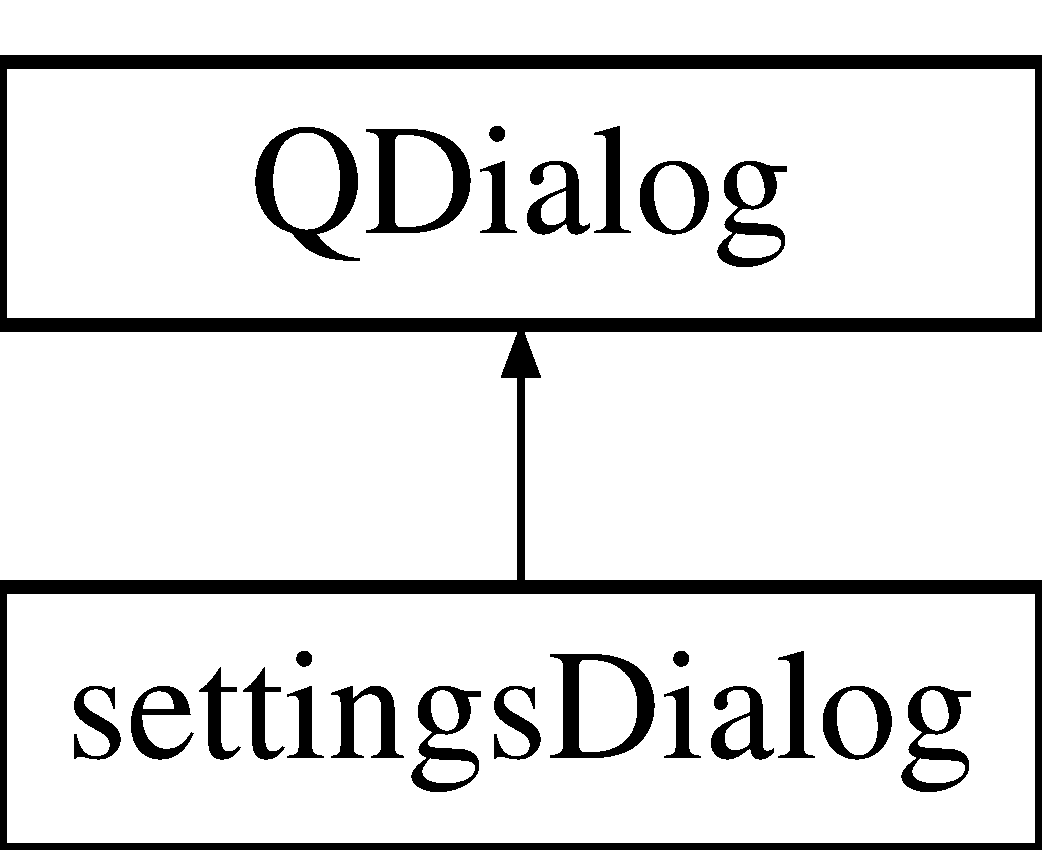
\includegraphics[height=2.000000cm]{classsettings_dialog}
\end{center}
\end{figure}
\subsection*{Signals}
\begin{DoxyCompactItemize}
\item 
\mbox{\Hypertarget{classsettings_dialog_afc5e121ba37f12221754a9e76172a82f}\label{classsettings_dialog_afc5e121ba37f12221754a9e76172a82f}} 
void {\bfseries scene\+Invalid} ()
\item 
\mbox{\Hypertarget{classsettings_dialog_a4b484584139b25437d8cb7218cf78a3c}\label{classsettings_dialog_a4b484584139b25437d8cb7218cf78a3c}} 
void {\bfseries set\+Background\+Colour} (Q\+Color colour)
\item 
\mbox{\Hypertarget{classsettings_dialog_a2f3b6b8dc939f18ae86b54d8ef86da56}\label{classsettings_dialog_a2f3b6b8dc939f18ae86b54d8ef86da56}} 
void {\bfseries save\+Directory\+Has\+Changed} ()
\end{DoxyCompactItemize}
\subsection*{Public Member Functions}
\begin{DoxyCompactItemize}
\item 
\mbox{\Hypertarget{classsettings_dialog_abe3d7f1c14fb45723918ae6bd0f999fa}\label{classsettings_dialog_abe3d7f1c14fb45723918ae6bd0f999fa}} 
{\bfseries settings\+Dialog} (Q\+Widget $\ast$parent=0)
\item 
\mbox{\Hypertarget{classsettings_dialog_a12dcaa04ce60f151ae7b77ce5ce2610d}\label{classsettings_dialog_a12dcaa04ce60f151ae7b77ce5ce2610d}} 
void {\bfseries show\+Event} (Q\+Show\+Event $\ast$event)
\item 
\mbox{\Hypertarget{classsettings_dialog_a6f5b6ea59e6a2de876fee96f0a5501da}\label{classsettings_dialog_a6f5b6ea59e6a2de876fee96f0a5501da}} 
void {\bfseries set\+Button\+Colour} (Q\+Push\+Button $\ast$button\+Pushed, Q\+Color colour)
\item 
\mbox{\Hypertarget{classsettings_dialog_afca53b725fce559f74266bb39657da6b}\label{classsettings_dialog_afca53b725fce559f74266bb39657da6b}} 
void {\bfseries apply\+Settings} ()
\item 
\mbox{\Hypertarget{classsettings_dialog_a982beae131fefc2788432b192ec343c7}\label{classsettings_dialog_a982beae131fefc2788432b192ec343c7}} 
void \mbox{\hyperlink{classsettings_dialog_a982beae131fefc2788432b192ec343c7}{load\+Values}} ()
\begin{DoxyCompactList}\small\item\em \mbox{\hyperlink{classsettings_dialog_a982beae131fefc2788432b192ec343c7}{settings\+Dialog\+::load\+Values}} This function takes the settings values that are needed for this dialog and stores them in a map where they can be edited without effecting the settings actual value. \end{DoxyCompactList}\end{DoxyCompactItemize}


The documentation for this class was generated from the following files\+:\begin{DoxyCompactItemize}
\item 
/\+Users/lukehutton/\+One\+Drive -\/ University of Leeds/\+University/\+Computer Science/\+Internship/moebinv-\/gui/include/settingsdialog.\+h\item 
/\+Users/lukehutton/\+One\+Drive -\/ University of Leeds/\+University/\+Computer Science/\+Internship/moebinv-\/gui/src/settingsdialog.\+cpp\end{DoxyCompactItemize}

\hypertarget{class_ui_1_1settings_dialog}{}\section{Ui\+:\+:settings\+Dialog Class Reference}
\label{class_ui_1_1settings_dialog}\index{Ui\+::settings\+Dialog@{Ui\+::settings\+Dialog}}
Inheritance diagram for Ui\+:\+:settings\+Dialog\+:\begin{figure}[H]
\begin{center}
\leavevmode
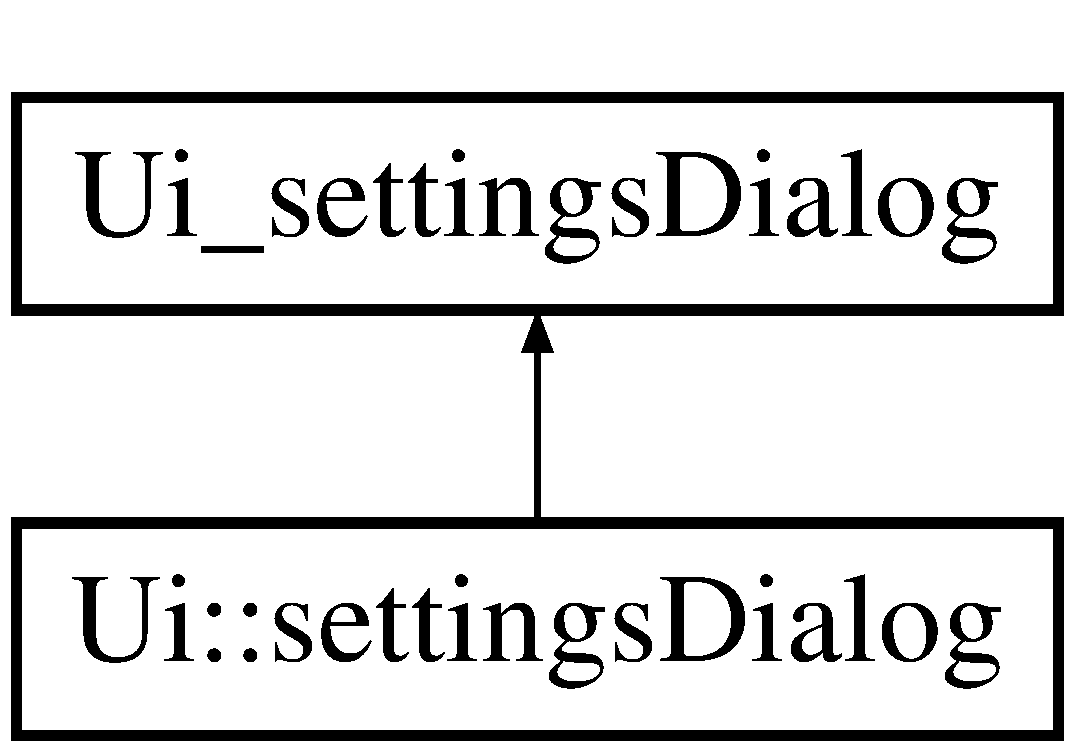
\includegraphics[height=2.000000cm]{class_ui_1_1settings_dialog}
\end{center}
\end{figure}
\subsection*{Additional Inherited Members}


The documentation for this class was generated from the following file\+:\begin{DoxyCompactItemize}
\item 
/\+Users/lukehutton/\+One\+Drive -\/ University of Leeds/\+University/\+Computer Science/\+Internship/moebinv-\/gui/moebinv-\/gui-\/build/ui\+\_\+settingsdialog.\+h\end{DoxyCompactItemize}

\hypertarget{structslide_param}{}\section{slide\+Param Struct Reference}
\label{structslide_param}\index{slide\+Param@{slide\+Param}}


{\ttfamily \#include $<$vis.\+h$>$}

\subsection*{Public Attributes}
\begin{DoxyCompactItemize}
\item 
string \mbox{\hyperlink{structslide_param_aff2f7e9ee5cf79eff9bb1dcb72cec41e}{key}}
\item 
int \mbox{\hyperlink{structslide_param_a573b67ecfcd670121b0fa2f7317ab2d6}{trans}}
\item 
int \mbox{\hyperlink{structslide_param_a742d4e9be7b5c16734b17a2d55b555c3}{group}}
\end{DoxyCompactItemize}


\subsection{Detailed Description}
stores data about the parameters of slideshow mode specified by the user 

\subsection{Member Data Documentation}
\mbox{\Hypertarget{structslide_param_a742d4e9be7b5c16734b17a2d55b555c3}\label{structslide_param_a742d4e9be7b5c16734b17a2d55b555c3}} 
\index{slide\+Param@{slide\+Param}!group@{group}}
\index{group@{group}!slide\+Param@{slide\+Param}}
\subsubsection{\texorpdfstring{group}{group}}
{\footnotesize\ttfamily int slide\+Param\+::group}

group type, 0 if individual, 1 if pair. \mbox{\Hypertarget{structslide_param_aff2f7e9ee5cf79eff9bb1dcb72cec41e}\label{structslide_param_aff2f7e9ee5cf79eff9bb1dcb72cec41e}} 
\index{slide\+Param@{slide\+Param}!key@{key}}
\index{key@{key}!slide\+Param@{slide\+Param}}
\subsubsection{\texorpdfstring{key}{key}}
{\footnotesize\ttfamily string slide\+Param\+::key}

key value of slideshow. \mbox{\Hypertarget{structslide_param_a573b67ecfcd670121b0fa2f7317ab2d6}\label{structslide_param_a573b67ecfcd670121b0fa2f7317ab2d6}} 
\index{slide\+Param@{slide\+Param}!trans@{trans}}
\index{trans@{trans}!slide\+Param@{slide\+Param}}
\subsubsection{\texorpdfstring{trans}{trans}}
{\footnotesize\ttfamily int slide\+Param\+::trans}

transition type, 0 if keystroke, 1 if time. 

The documentation for this struct was generated from the following file\+:\begin{DoxyCompactItemize}
\item 
/\+Users/lukehutton/\+One\+Drive -\/ University of Leeds/\+University/\+Computer Science/\+Internship/moebinv-\/gui/lib/moebinv-\/3.\+2/cycle3\+D-\/visualiser/vis.\+h\end{DoxyCompactItemize}

\hypertarget{class_moeb_inv_1_1subfigure}{}\section{Moeb\+Inv\+:\+:subfigure Class Reference}
\label{class_moeb_inv_1_1subfigure}\index{Moeb\+Inv\+::subfigure@{Moeb\+Inv\+::subfigure}}
Inheritance diagram for Moeb\+Inv\+:\+:subfigure\+:\begin{figure}[H]
\begin{center}
\leavevmode
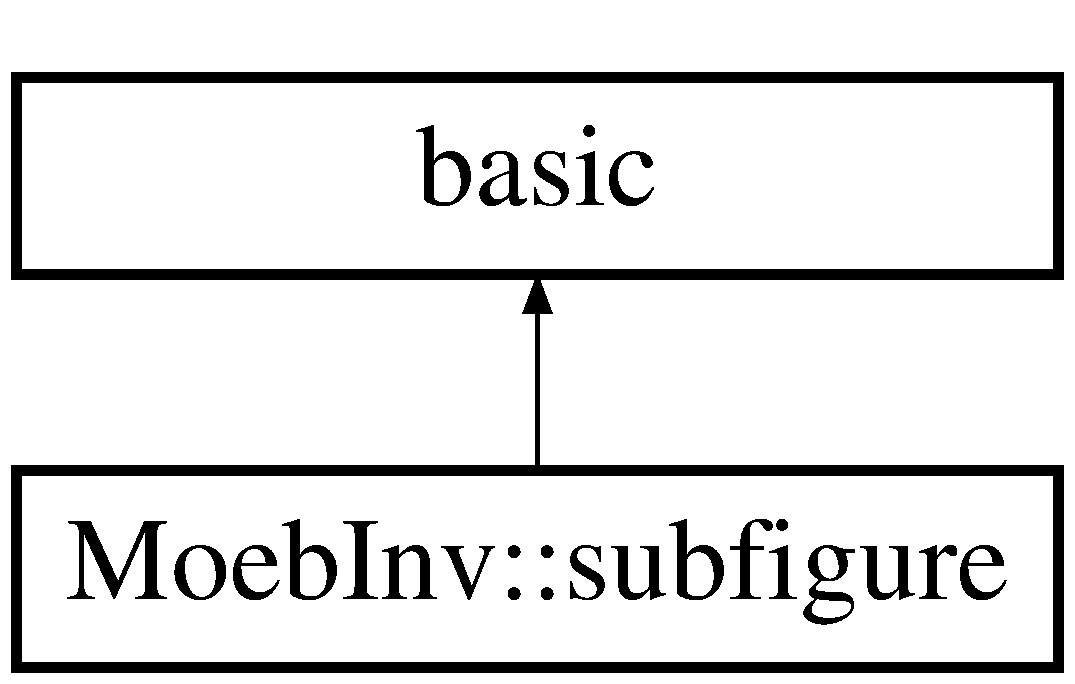
\includegraphics[height=2.000000cm]{class_moeb_inv_1_1subfigure}
\end{center}
\end{figure}
\subsection*{Public Member Functions}
\begin{DoxyCompactItemize}
\item 
\mbox{\Hypertarget{class_moeb_inv_1_1subfigure_ab64c52c45f0b7a0bed82b13aeb2418b2}\label{class_moeb_inv_1_1subfigure_ab64c52c45f0b7a0bed82b13aeb2418b2}} 
{\bfseries subfigure} (const ex \&F, const ex \&L)
\item 
\mbox{\Hypertarget{class_moeb_inv_1_1subfigure_ac873c29bb1b1a0b70b29cddf71193834}\label{class_moeb_inv_1_1subfigure_ac873c29bb1b1a0b70b29cddf71193834}} 
ex {\bfseries subs} (const exmap \&em, unsigned options=0) const
\end{DoxyCompactItemize}
\subsection*{Protected Member Functions}
\begin{DoxyCompactItemize}
\item 
\mbox{\Hypertarget{class_moeb_inv_1_1subfigure_a918353b34513df293690b9cc52b054e4}\label{class_moeb_inv_1_1subfigure_a918353b34513df293690b9cc52b054e4}} 
ex {\bfseries get\+\_\+parlist} () const
\item 
\mbox{\Hypertarget{class_moeb_inv_1_1subfigure_a867136abf548a648d6e2520276e683b3}\label{class_moeb_inv_1_1subfigure_a867136abf548a648d6e2520276e683b3}} 
ex {\bfseries get\+\_\+subf} () const
\item 
\mbox{\Hypertarget{class_moeb_inv_1_1subfigure_a4ebd74b08b23f3486c4e9946b2126976}\label{class_moeb_inv_1_1subfigure_a4ebd74b08b23f3486c4e9946b2126976}} 
return\+\_\+type\+\_\+t {\bfseries return\+\_\+type\+\_\+tinfo} () const
\item 
\mbox{\Hypertarget{class_moeb_inv_1_1subfigure_a6bff7c7a0c383e99c633a7dd82d24ede}\label{class_moeb_inv_1_1subfigure_a6bff7c7a0c383e99c633a7dd82d24ede}} 
void {\bfseries do\+\_\+print} (const print\+\_\+dflt \&con, unsigned level) const
\item 
\mbox{\Hypertarget{class_moeb_inv_1_1subfigure_a00ca520915569473c9fde98383feaacb}\label{class_moeb_inv_1_1subfigure_a00ca520915569473c9fde98383feaacb}} 
void {\bfseries do\+\_\+print\+\_\+tree} (const print\+\_\+tree \&con, unsigned level) const
\item 
\mbox{\Hypertarget{class_moeb_inv_1_1subfigure_ac6df4d0f4fca396760208e88db553878}\label{class_moeb_inv_1_1subfigure_ac6df4d0f4fca396760208e88db553878}} 
void {\bfseries archive} (archive\+\_\+node \&n) const
\item 
\mbox{\Hypertarget{class_moeb_inv_1_1subfigure_a1bbb1181211b89637ae13f6c9b9ca081}\label{class_moeb_inv_1_1subfigure_a1bbb1181211b89637ae13f6c9b9ca081}} 
void {\bfseries read\+\_\+archive} (const archive\+\_\+node \&n, lst \&sym\+\_\+lst)
\end{DoxyCompactItemize}
\subsection*{Protected Attributes}
\begin{DoxyCompactItemize}
\item 
\mbox{\Hypertarget{class_moeb_inv_1_1subfigure_abfb9102f879a82bbfe67b73af6f95db7}\label{class_moeb_inv_1_1subfigure_abfb9102f879a82bbfe67b73af6f95db7}} 
ex {\bfseries subf}
\item 
\mbox{\Hypertarget{class_moeb_inv_1_1subfigure_ae1c45cc944264ac922f4a9ea43a82ed5}\label{class_moeb_inv_1_1subfigure_ae1c45cc944264ac922f4a9ea43a82ed5}} 
lst {\bfseries parlist}
\end{DoxyCompactItemize}
\subsection*{Friends}
\begin{DoxyCompactItemize}
\item 
\mbox{\Hypertarget{class_moeb_inv_1_1subfigure_ab1135e74268f9c17da7328c07edd8b09}\label{class_moeb_inv_1_1subfigure_ab1135e74268f9c17da7328c07edd8b09}} 
class {\bfseries cycle\+\_\+node}
\item 
\mbox{\Hypertarget{class_moeb_inv_1_1subfigure_ac46ec1ee00928c9cde5b63a7edba7b7a}\label{class_moeb_inv_1_1subfigure_ac46ec1ee00928c9cde5b63a7edba7b7a}} 
class {\bfseries figure}
\end{DoxyCompactItemize}


The documentation for this class was generated from the following file\+:\begin{DoxyCompactItemize}
\item 
/\+Users/lukehutton/\+One\+Drive -\/ University of Leeds/\+University/\+Computer Science/\+Internship/moebinv-\/gui/lib/moebinv-\/3.\+2/include/figure.\+h\end{DoxyCompactItemize}

\hypertarget{classtree_model}{}\section{tree\+Model Class Reference}
\label{classtree_model}\index{tree\+Model@{tree\+Model}}
Inheritance diagram for tree\+Model\+:\begin{figure}[H]
\begin{center}
\leavevmode
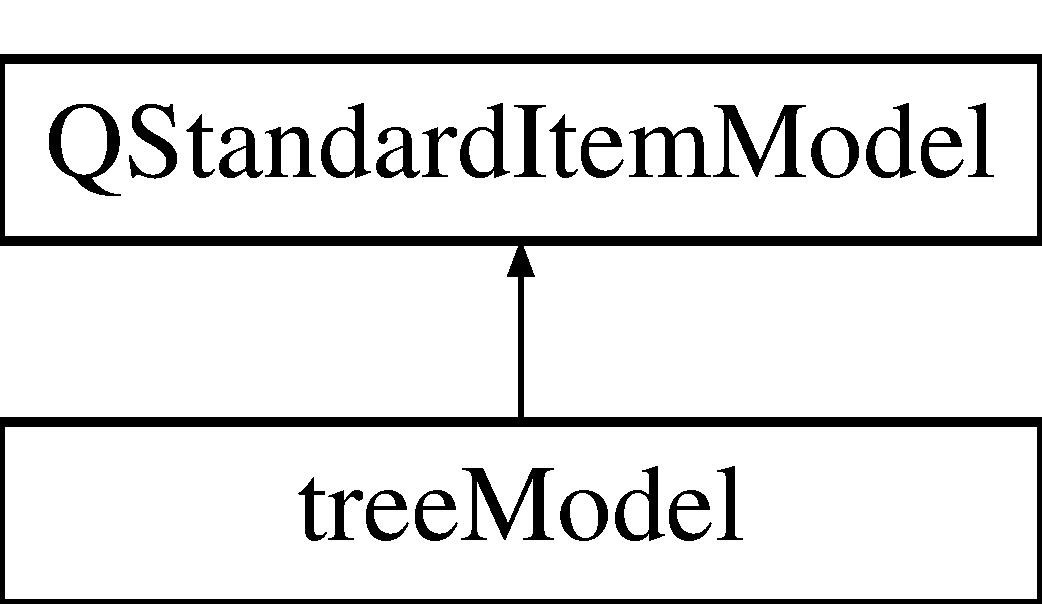
\includegraphics[height=2.000000cm]{classtree_model}
\end{center}
\end{figure}
\subsection*{Public Member Functions}
\begin{DoxyCompactItemize}
\item 
\mbox{\Hypertarget{classtree_model_ad3539d2628250edeea80fe4ffe0a80fa}\label{classtree_model_ad3539d2628250edeea80fe4ffe0a80fa}} 
{\bfseries tree\+Model} (Q\+Object $\ast$parent=0)
\end{DoxyCompactItemize}


The documentation for this class was generated from the following files\+:\begin{DoxyCompactItemize}
\item 
/\+Users/lukehutton/\+One\+Drive -\/ University of Leeds/\+University/\+Computer Science/\+Internship/moebinv-\/gui/include/treemodel.\+h\item 
/\+Users/lukehutton/\+One\+Drive -\/ University of Leeds/\+University/\+Computer Science/\+Internship/moebinv-\/gui/src/treemodel.\+cpp\end{DoxyCompactItemize}

\hypertarget{class_ui__define_cycle_dialog}{}\section{Ui\+\_\+define\+Cycle\+Dialog Class Reference}
\label{class_ui__define_cycle_dialog}\index{Ui\+\_\+define\+Cycle\+Dialog@{Ui\+\_\+define\+Cycle\+Dialog}}
Inheritance diagram for Ui\+\_\+define\+Cycle\+Dialog\+:\begin{figure}[H]
\begin{center}
\leavevmode
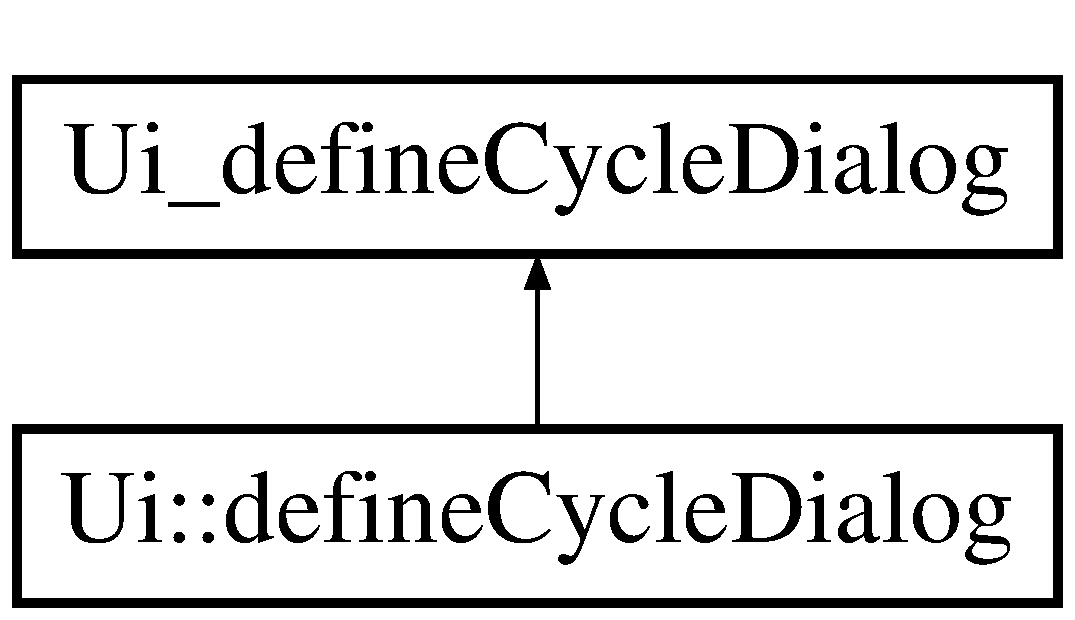
\includegraphics[height=2.000000cm]{class_ui__define_cycle_dialog}
\end{center}
\end{figure}
\subsection*{Public Member Functions}
\begin{DoxyCompactItemize}
\item 
\mbox{\Hypertarget{class_ui__define_cycle_dialog_a023518fe6242d0a90494ecbb897dd9ac}\label{class_ui__define_cycle_dialog_a023518fe6242d0a90494ecbb897dd9ac}} 
void {\bfseries setup\+Ui} (Q\+Dialog $\ast$\mbox{\hyperlink{classdefine_cycle_dialog}{define\+Cycle\+Dialog}})
\item 
\mbox{\Hypertarget{class_ui__define_cycle_dialog_ab6b479d0332ab9a2e9ccc6ee3416bb97}\label{class_ui__define_cycle_dialog_ab6b479d0332ab9a2e9ccc6ee3416bb97}} 
void {\bfseries retranslate\+Ui} (Q\+Dialog $\ast$\mbox{\hyperlink{classdefine_cycle_dialog}{define\+Cycle\+Dialog}})
\end{DoxyCompactItemize}
\subsection*{Public Attributes}
\begin{DoxyCompactItemize}
\item 
\mbox{\Hypertarget{class_ui__define_cycle_dialog_ac2a973c429b8357847bf4cda2a45c9ff}\label{class_ui__define_cycle_dialog_ac2a973c429b8357847bf4cda2a45c9ff}} 
Q\+V\+Box\+Layout $\ast$ {\bfseries vertical\+Layout\+\_\+3}
\item 
\mbox{\Hypertarget{class_ui__define_cycle_dialog_a8341722258f5c60291744e1feb431bce}\label{class_ui__define_cycle_dialog_a8341722258f5c60291744e1feb431bce}} 
Q\+Tab\+Widget $\ast$ {\bfseries tab\+Widget}
\item 
\mbox{\Hypertarget{class_ui__define_cycle_dialog_afe9cf82080d34f1bc821c7d3e2b1064d}\label{class_ui__define_cycle_dialog_afe9cf82080d34f1bc821c7d3e2b1064d}} 
Q\+Widget $\ast$ {\bfseries tab\+Values}
\item 
\mbox{\Hypertarget{class_ui__define_cycle_dialog_a2e44f950f76b27f972dfea6230d12713}\label{class_ui__define_cycle_dialog_a2e44f950f76b27f972dfea6230d12713}} 
Q\+V\+Box\+Layout $\ast$ {\bfseries vertical\+Layout\+\_\+2}
\item 
\mbox{\Hypertarget{class_ui__define_cycle_dialog_a608df977a3a1c84586b3fb842bb171dc}\label{class_ui__define_cycle_dialog_a608df977a3a1c84586b3fb842bb171dc}} 
Q\+H\+Box\+Layout $\ast$ {\bfseries horizontal\+Layout}
\item 
\mbox{\Hypertarget{class_ui__define_cycle_dialog_a2441722611a27b6c3ac821ba7e82dfe3}\label{class_ui__define_cycle_dialog_a2441722611a27b6c3ac821ba7e82dfe3}} 
Q\+Spacer\+Item $\ast$ {\bfseries horizontal\+Spacer\+\_\+3}
\item 
\mbox{\Hypertarget{class_ui__define_cycle_dialog_a9217f34088f20f107c710da69275d1ed}\label{class_ui__define_cycle_dialog_a9217f34088f20f107c710da69275d1ed}} 
Q\+Label $\ast$ {\bfseries label\+\_\+3}
\item 
\mbox{\Hypertarget{class_ui__define_cycle_dialog_aa5960dd55cf7ea412bab9d5e1929c3a9}\label{class_ui__define_cycle_dialog_aa5960dd55cf7ea412bab9d5e1929c3a9}} 
Q\+Line\+Edit $\ast$ {\bfseries line\+Edit\+\_\+1}
\item 
\mbox{\Hypertarget{class_ui__define_cycle_dialog_aa3688c0abd181e61e1fd13daece711b5}\label{class_ui__define_cycle_dialog_aa3688c0abd181e61e1fd13daece711b5}} 
Q\+Spacer\+Item $\ast$ {\bfseries horizontal\+Spacer\+\_\+4}
\item 
\mbox{\Hypertarget{class_ui__define_cycle_dialog_a121d9b5a7a2d5cab23a6a05c08de003a}\label{class_ui__define_cycle_dialog_a121d9b5a7a2d5cab23a6a05c08de003a}} 
Q\+H\+Box\+Layout $\ast$ {\bfseries horizontal\+Layout\+\_\+2}
\item 
\mbox{\Hypertarget{class_ui__define_cycle_dialog_a127f945f6fb4d7a4b04e779f6430390d}\label{class_ui__define_cycle_dialog_a127f945f6fb4d7a4b04e779f6430390d}} 
Q\+Spacer\+Item $\ast$ {\bfseries horizontal\+Spacer}
\item 
\mbox{\Hypertarget{class_ui__define_cycle_dialog_a5d9740251cf9b4070346923008408005}\label{class_ui__define_cycle_dialog_a5d9740251cf9b4070346923008408005}} 
Q\+Label $\ast$ {\bfseries label}
\item 
\mbox{\Hypertarget{class_ui__define_cycle_dialog_a7fd0d74a07d9ddef9c7e02338e8fda67}\label{class_ui__define_cycle_dialog_a7fd0d74a07d9ddef9c7e02338e8fda67}} 
Q\+Line\+Edit $\ast$ {\bfseries line\+Edit\+\_\+2}
\item 
\mbox{\Hypertarget{class_ui__define_cycle_dialog_a33699becdc8a75f39ab46d514d4560fc}\label{class_ui__define_cycle_dialog_a33699becdc8a75f39ab46d514d4560fc}} 
Q\+Spacer\+Item $\ast$ {\bfseries horizontal\+Spacer\+\_\+2}
\item 
\mbox{\Hypertarget{class_ui__define_cycle_dialog_a098d7c18c9dd398ce64afe12be51543c}\label{class_ui__define_cycle_dialog_a098d7c18c9dd398ce64afe12be51543c}} 
Q\+H\+Box\+Layout $\ast$ {\bfseries horizontal\+Layout\+\_\+3}
\item 
\mbox{\Hypertarget{class_ui__define_cycle_dialog_a9aa938d116df1ce366a72d66d3f75840}\label{class_ui__define_cycle_dialog_a9aa938d116df1ce366a72d66d3f75840}} 
Q\+Spacer\+Item $\ast$ {\bfseries horizontal\+Spacer\+\_\+5}
\item 
\mbox{\Hypertarget{class_ui__define_cycle_dialog_ad259fb66ce1b09bf92ad13d9e116b253}\label{class_ui__define_cycle_dialog_ad259fb66ce1b09bf92ad13d9e116b253}} 
Q\+Label $\ast$ {\bfseries label\+\_\+2}
\item 
\mbox{\Hypertarget{class_ui__define_cycle_dialog_add3cf25304b9c6a6c4bcb2ae20da67b3}\label{class_ui__define_cycle_dialog_add3cf25304b9c6a6c4bcb2ae20da67b3}} 
Q\+Line\+Edit $\ast$ {\bfseries line\+Edit\+\_\+3}
\item 
\mbox{\Hypertarget{class_ui__define_cycle_dialog_a55be67bb153a9a1dd8a2bcc30eb798a2}\label{class_ui__define_cycle_dialog_a55be67bb153a9a1dd8a2bcc30eb798a2}} 
Q\+Spacer\+Item $\ast$ {\bfseries horizontal\+Spacer\+\_\+6}
\item 
\mbox{\Hypertarget{class_ui__define_cycle_dialog_ad9f452c726da3b9705f58ede8cfdeb2d}\label{class_ui__define_cycle_dialog_ad9f452c726da3b9705f58ede8cfdeb2d}} 
Q\+H\+Box\+Layout $\ast$ {\bfseries horizontal\+Layout\+\_\+4}
\item 
\mbox{\Hypertarget{class_ui__define_cycle_dialog_abe517a13c8e5a613d534992abbbf85ce}\label{class_ui__define_cycle_dialog_abe517a13c8e5a613d534992abbbf85ce}} 
Q\+Spacer\+Item $\ast$ {\bfseries horizontal\+Spacer\+\_\+7}
\item 
\mbox{\Hypertarget{class_ui__define_cycle_dialog_ab660392d534326c4ecab689ae041f37b}\label{class_ui__define_cycle_dialog_ab660392d534326c4ecab689ae041f37b}} 
Q\+Label $\ast$ {\bfseries label\+\_\+4}
\item 
\mbox{\Hypertarget{class_ui__define_cycle_dialog_aae21ab9ac566059dee36fa8a154d7f1a}\label{class_ui__define_cycle_dialog_aae21ab9ac566059dee36fa8a154d7f1a}} 
Q\+Line\+Edit $\ast$ {\bfseries line\+Edit\+\_\+4}
\item 
\mbox{\Hypertarget{class_ui__define_cycle_dialog_afbc4007ba8f3b553560ee3da5873120b}\label{class_ui__define_cycle_dialog_afbc4007ba8f3b553560ee3da5873120b}} 
Q\+Spacer\+Item $\ast$ {\bfseries horizontal\+Spacer\+\_\+8}
\item 
\mbox{\Hypertarget{class_ui__define_cycle_dialog_a912f00d8c89ac32ba3774fb8106420f3}\label{class_ui__define_cycle_dialog_a912f00d8c89ac32ba3774fb8106420f3}} 
Q\+Widget $\ast$ {\bfseries tab\+Center}
\item 
\mbox{\Hypertarget{class_ui__define_cycle_dialog_a5e0d16d30bcb9ff54944ffc75d965b7d}\label{class_ui__define_cycle_dialog_a5e0d16d30bcb9ff54944ffc75d965b7d}} 
Q\+V\+Box\+Layout $\ast$ {\bfseries vertical\+Layout}
\item 
\mbox{\Hypertarget{class_ui__define_cycle_dialog_ac6483121f806471d84de6ba86e61921b}\label{class_ui__define_cycle_dialog_ac6483121f806471d84de6ba86e61921b}} 
Q\+Group\+Box $\ast$ {\bfseries group\+Box}
\item 
\mbox{\Hypertarget{class_ui__define_cycle_dialog_a4406dcb26a55c866b3cfc269366d9294}\label{class_ui__define_cycle_dialog_a4406dcb26a55c866b3cfc269366d9294}} 
Q\+V\+Box\+Layout $\ast$ {\bfseries vertical\+Layout\+\_\+4}
\item 
\mbox{\Hypertarget{class_ui__define_cycle_dialog_a25296210e8cbc4a2eacc58d7420ac53c}\label{class_ui__define_cycle_dialog_a25296210e8cbc4a2eacc58d7420ac53c}} 
Q\+H\+Box\+Layout $\ast$ {\bfseries horizontal\+Layout\+\_\+6}
\item 
\mbox{\Hypertarget{class_ui__define_cycle_dialog_a2ec5867b62c0e11abcbb50fa984c1f94}\label{class_ui__define_cycle_dialog_a2ec5867b62c0e11abcbb50fa984c1f94}} 
Q\+Label $\ast$ {\bfseries label\+\_\+6}
\item 
\mbox{\Hypertarget{class_ui__define_cycle_dialog_a3d5520f021e4be628878c16356d867e4}\label{class_ui__define_cycle_dialog_a3d5520f021e4be628878c16356d867e4}} 
Q\+Line\+Edit $\ast$ {\bfseries line\+Edit\+\_\+5}
\item 
\mbox{\Hypertarget{class_ui__define_cycle_dialog_a9eb7ed48f73134128d9c641db721d41f}\label{class_ui__define_cycle_dialog_a9eb7ed48f73134128d9c641db721d41f}} 
Q\+Spacer\+Item $\ast$ {\bfseries horizontal\+Spacer\+\_\+11}
\item 
\mbox{\Hypertarget{class_ui__define_cycle_dialog_a03c84f7955219dc3905bb5ca4f0af39e}\label{class_ui__define_cycle_dialog_a03c84f7955219dc3905bb5ca4f0af39e}} 
Q\+H\+Box\+Layout $\ast$ {\bfseries horizontal\+Layout\+\_\+5}
\item 
\mbox{\Hypertarget{class_ui__define_cycle_dialog_a6f26b71d4b3e5be6f5561d045125198c}\label{class_ui__define_cycle_dialog_a6f26b71d4b3e5be6f5561d045125198c}} 
Q\+Label $\ast$ {\bfseries label\+\_\+5}
\item 
\mbox{\Hypertarget{class_ui__define_cycle_dialog_aa19a105e0b9670c923be42cf953a55e0}\label{class_ui__define_cycle_dialog_aa19a105e0b9670c923be42cf953a55e0}} 
Q\+Line\+Edit $\ast$ {\bfseries line\+Edit\+\_\+6}
\item 
\mbox{\Hypertarget{class_ui__define_cycle_dialog_ab4de9ae4f5fb1e738c22bd8d2fbb8571}\label{class_ui__define_cycle_dialog_ab4de9ae4f5fb1e738c22bd8d2fbb8571}} 
Q\+Spacer\+Item $\ast$ {\bfseries horizontal\+Spacer\+\_\+10}
\item 
\mbox{\Hypertarget{class_ui__define_cycle_dialog_a103cdf5b651b17a0716c66891b5a11df}\label{class_ui__define_cycle_dialog_a103cdf5b651b17a0716c66891b5a11df}} 
Q\+H\+Box\+Layout $\ast$ {\bfseries horizontal\+Layout\+\_\+7}
\item 
\mbox{\Hypertarget{class_ui__define_cycle_dialog_a7c005f2e7df6caa5e9b81ed1716c0382}\label{class_ui__define_cycle_dialog_a7c005f2e7df6caa5e9b81ed1716c0382}} 
Q\+Label $\ast$ {\bfseries label\+\_\+7}
\item 
\mbox{\Hypertarget{class_ui__define_cycle_dialog_ae3e3d1bd890adbe23502349a6b2fe90a}\label{class_ui__define_cycle_dialog_ae3e3d1bd890adbe23502349a6b2fe90a}} 
Q\+Line\+Edit $\ast$ {\bfseries line\+Edit\+\_\+7}
\item 
\mbox{\Hypertarget{class_ui__define_cycle_dialog_a56c94e17b5226b6c00588a9085e4ee89}\label{class_ui__define_cycle_dialog_a56c94e17b5226b6c00588a9085e4ee89}} 
Q\+Spacer\+Item $\ast$ {\bfseries horizontal\+Spacer\+\_\+9}
\item 
\mbox{\Hypertarget{class_ui__define_cycle_dialog_ae1d3f2442bdfe35eccc053c09694f7f2}\label{class_ui__define_cycle_dialog_ae1d3f2442bdfe35eccc053c09694f7f2}} 
Q\+Dialog\+Button\+Box $\ast$ {\bfseries button\+Box}
\end{DoxyCompactItemize}


The documentation for this class was generated from the following file\+:\begin{DoxyCompactItemize}
\item 
/\+Users/lukehutton/\+One\+Drive -\/ University of Leeds/\+University/\+Computer Science/\+Internship/moebinv-\/gui/moebinv-\/gui-\/build/ui\+\_\+definecycledialog.\+h\end{DoxyCompactItemize}

\hypertarget{class_ui__help_dialog}{}\section{Ui\+\_\+help\+Dialog Class Reference}
\label{class_ui__help_dialog}\index{Ui\+\_\+help\+Dialog@{Ui\+\_\+help\+Dialog}}
Inheritance diagram for Ui\+\_\+help\+Dialog\+:\begin{figure}[H]
\begin{center}
\leavevmode
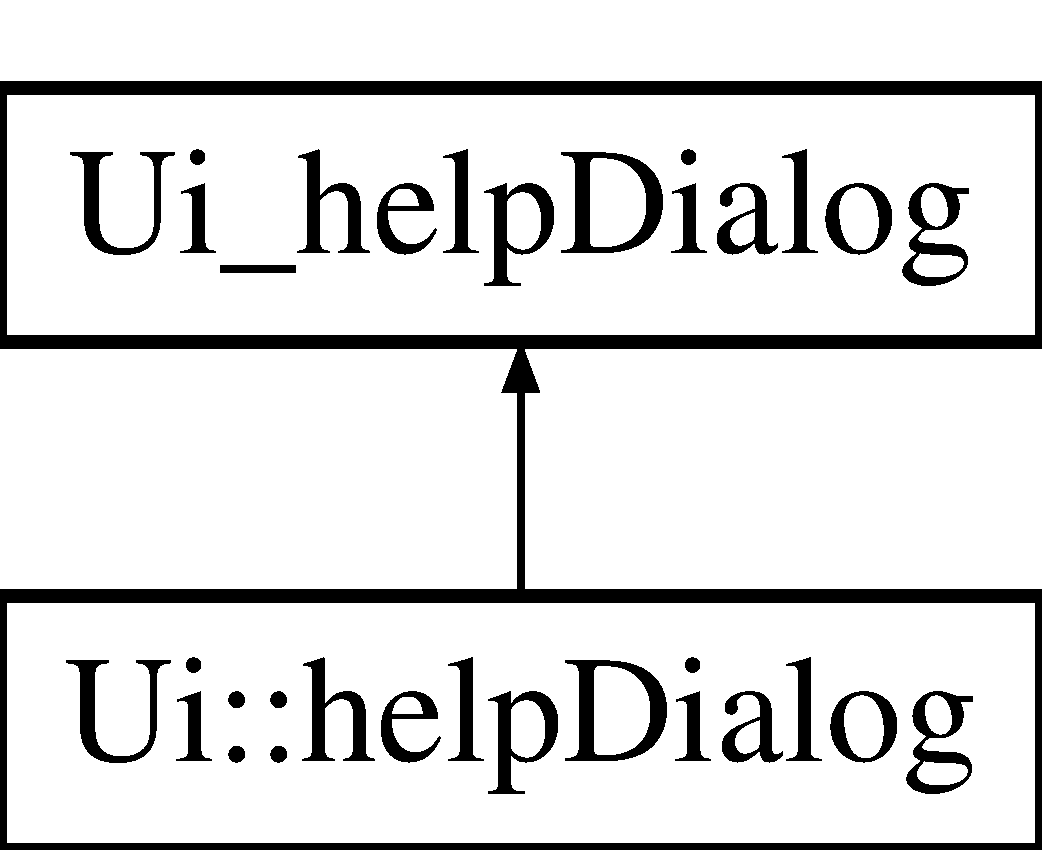
\includegraphics[height=2.000000cm]{class_ui__help_dialog}
\end{center}
\end{figure}
\subsection*{Public Member Functions}
\begin{DoxyCompactItemize}
\item 
\mbox{\Hypertarget{class_ui__help_dialog_a4074ac03760c68b2a4d9ba5e9aa47f4b}\label{class_ui__help_dialog_a4074ac03760c68b2a4d9ba5e9aa47f4b}} 
void {\bfseries setup\+Ui} (Q\+Dialog $\ast$\mbox{\hyperlink{classhelp_dialog}{help\+Dialog}})
\item 
\mbox{\Hypertarget{class_ui__help_dialog_a2f67a7a9b16bb22a264d312234c7e60d}\label{class_ui__help_dialog_a2f67a7a9b16bb22a264d312234c7e60d}} 
void {\bfseries retranslate\+Ui} (Q\+Dialog $\ast$\mbox{\hyperlink{classhelp_dialog}{help\+Dialog}})
\end{DoxyCompactItemize}
\subsection*{Public Attributes}
\begin{DoxyCompactItemize}
\item 
\mbox{\Hypertarget{class_ui__help_dialog_a9a2ecc710af91e4b1e89a3d49e5a22c0}\label{class_ui__help_dialog_a9a2ecc710af91e4b1e89a3d49e5a22c0}} 
Q\+H\+Box\+Layout $\ast$ {\bfseries horizontal\+Layout}
\item 
\mbox{\Hypertarget{class_ui__help_dialog_a72aa819f279809b1c253f46bd2cec5dc}\label{class_ui__help_dialog_a72aa819f279809b1c253f46bd2cec5dc}} 
Q\+Splitter $\ast$ {\bfseries splitter}
\item 
\mbox{\Hypertarget{class_ui__help_dialog_a0c873833046066c8d4594e59905ad8d5}\label{class_ui__help_dialog_a0c873833046066c8d4594e59905ad8d5}} 
Q\+Tab\+Widget $\ast$ {\bfseries tab\+Widget}
\item 
\mbox{\Hypertarget{class_ui__help_dialog_ac04b5a0ba104077649c97b8ab07afc65}\label{class_ui__help_dialog_ac04b5a0ba104077649c97b8ab07afc65}} 
\mbox{\hyperlink{classhelp_browser}{help\+Browser}} $\ast$ {\bfseries text\+Browser}
\end{DoxyCompactItemize}


The documentation for this class was generated from the following file\+:\begin{DoxyCompactItemize}
\item 
/\+Users/lukehutton/\+One\+Drive -\/ University of Leeds/\+University/\+Computer Science/\+Internship/moebinv-\/gui/moebinv-\/gui-\/build/ui\+\_\+helpdialog.\+h\end{DoxyCompactItemize}

\hypertarget{class_ui___main_window}{}\section{Ui\+\_\+\+Main\+Window Class Reference}
\label{class_ui___main_window}\index{Ui\+\_\+\+Main\+Window@{Ui\+\_\+\+Main\+Window}}
Inheritance diagram for Ui\+\_\+\+Main\+Window\+:\begin{figure}[H]
\begin{center}
\leavevmode
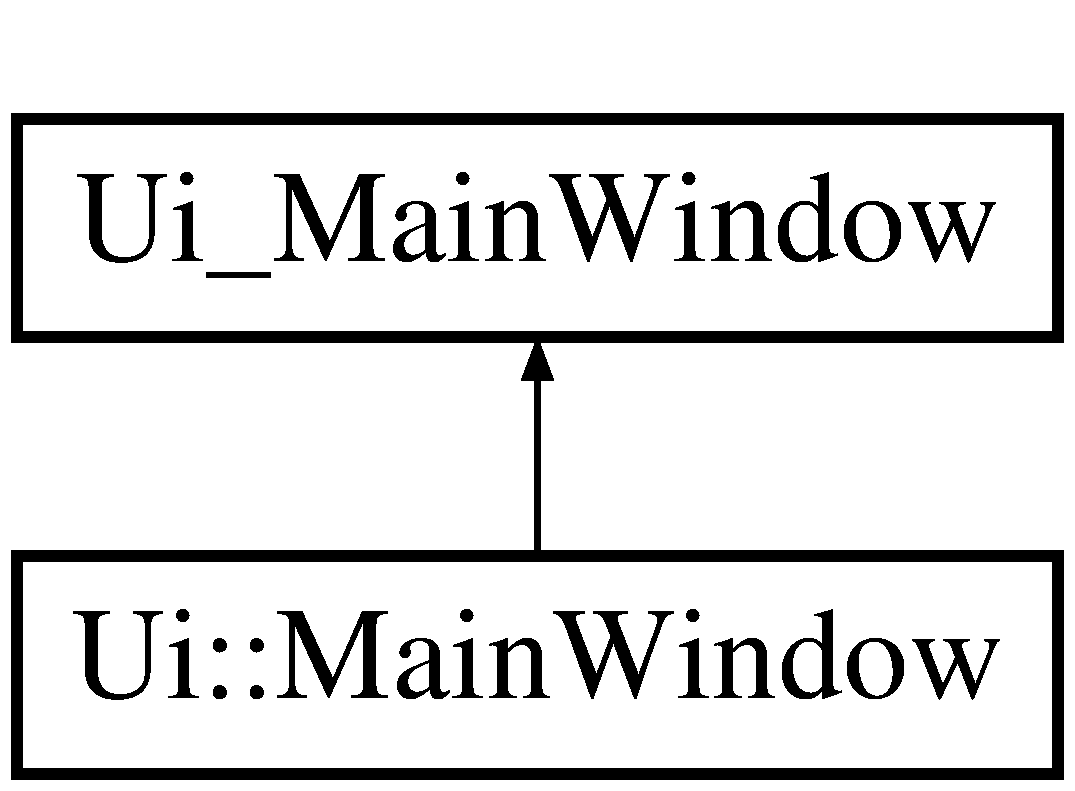
\includegraphics[height=2.000000cm]{class_ui___main_window}
\end{center}
\end{figure}
\subsection*{Public Member Functions}
\begin{DoxyCompactItemize}
\item 
\mbox{\Hypertarget{class_ui___main_window_acf4a0872c4c77d8f43a2ec66ed849b58}\label{class_ui___main_window_acf4a0872c4c77d8f43a2ec66ed849b58}} 
void {\bfseries setup\+Ui} (Q\+Main\+Window $\ast$\mbox{\hyperlink{class_main_window}{Main\+Window}})
\item 
\mbox{\Hypertarget{class_ui___main_window_a097dd160c3534a204904cb374412c618}\label{class_ui___main_window_a097dd160c3534a204904cb374412c618}} 
void {\bfseries retranslate\+Ui} (Q\+Main\+Window $\ast$\mbox{\hyperlink{class_main_window}{Main\+Window}})
\end{DoxyCompactItemize}
\subsection*{Public Attributes}
\begin{DoxyCompactItemize}
\item 
\mbox{\Hypertarget{class_ui___main_window_a9090620adfd867b72c5f445c83b8c0ec}\label{class_ui___main_window_a9090620adfd867b72c5f445c83b8c0ec}} 
Q\+Action $\ast$ {\bfseries action\+New}
\item 
\mbox{\Hypertarget{class_ui___main_window_a6e14788227f1a0dbc8cf983514685f3b}\label{class_ui___main_window_a6e14788227f1a0dbc8cf983514685f3b}} 
Q\+Action $\ast$ {\bfseries action\+Save}
\item 
\mbox{\Hypertarget{class_ui___main_window_a5772f39001f62b7f601aafe72caa10c0}\label{class_ui___main_window_a5772f39001f62b7f601aafe72caa10c0}} 
Q\+Action $\ast$ {\bfseries action\+Open}
\item 
\mbox{\Hypertarget{class_ui___main_window_aa2c71d96d12d8103436804c3fda3855d}\label{class_ui___main_window_aa2c71d96d12d8103436804c3fda3855d}} 
Q\+Action $\ast$ {\bfseries action\+Configuration}
\item 
\mbox{\Hypertarget{class_ui___main_window_a711ee49dc285749537d57e6756b1a0c3}\label{class_ui___main_window_a711ee49dc285749537d57e6756b1a0c3}} 
Q\+Action $\ast$ {\bfseries action\+User\+\_\+\+Manual}
\item 
\mbox{\Hypertarget{class_ui___main_window_abdf2b43167c2cd0d3405f90b8c30e934}\label{class_ui___main_window_abdf2b43167c2cd0d3405f90b8c30e934}} 
Q\+Action $\ast$ {\bfseries action\+About}
\item 
\mbox{\Hypertarget{class_ui___main_window_ab34717288693d70d787ff80f9ad3f633}\label{class_ui___main_window_ab34717288693d70d787ff80f9ad3f633}} 
Q\+Action $\ast$ {\bfseries action\+Create\+\_\+\+Cycle}
\item 
\mbox{\Hypertarget{class_ui___main_window_abfbd7004decc3b1240e9009b86c0500e}\label{class_ui___main_window_abfbd7004decc3b1240e9009b86c0500e}} 
Q\+Action $\ast$ {\bfseries action\+Pan}
\item 
\mbox{\Hypertarget{class_ui___main_window_a262b4df5530dbefe28c149fa86f140b2}\label{class_ui___main_window_a262b4df5530dbefe28c149fa86f140b2}} 
Q\+Action $\ast$ {\bfseries action\+Labels}
\item 
\mbox{\Hypertarget{class_ui___main_window_a30a8a79f7c40582f655109ebe2dcfcff}\label{class_ui___main_window_a30a8a79f7c40582f655109ebe2dcfcff}} 
Q\+Action $\ast$ {\bfseries actionzoom\+In}
\item 
\mbox{\Hypertarget{class_ui___main_window_a749319d9c2f86308f4559091acff6910}\label{class_ui___main_window_a749319d9c2f86308f4559091acff6910}} 
Q\+Action $\ast$ {\bfseries actionzoom\+Out}
\item 
\mbox{\Hypertarget{class_ui___main_window_ab922a617328dd984d45d82e8aa460d13}\label{class_ui___main_window_ab922a617328dd984d45d82e8aa460d13}} 
Q\+Action $\ast$ {\bfseries action\+Debug\+\_\+bounding\+\_\+rect}
\item 
\mbox{\Hypertarget{class_ui___main_window_a80f63d6b857721d1d102cd7ba5063878}\label{class_ui___main_window_a80f63d6b857721d1d102cd7ba5063878}} 
Q\+Action $\ast$ {\bfseries action\+Define\+\_\+by\+\_\+center\+\_\+and\+\_\+radius\+\_\+squared}
\item 
\mbox{\Hypertarget{class_ui___main_window_a0b0a125bc543f541304b27a09559e72d}\label{class_ui___main_window_a0b0a125bc543f541304b27a09559e72d}} 
Q\+Action $\ast$ {\bfseries action\+Define\+\_\+by\+\_\+values}
\item 
\mbox{\Hypertarget{class_ui___main_window_a1087883ccba9316d3703d696746101d3}\label{class_ui___main_window_a1087883ccba9316d3703d696746101d3}} 
Q\+Action $\ast$ {\bfseries action\+Define\+\_\+cycle}
\item 
\mbox{\Hypertarget{class_ui___main_window_a1e11ac34a44aeff9d0f198e5f2537dab}\label{class_ui___main_window_a1e11ac34a44aeff9d0f198e5f2537dab}} 
Q\+Action $\ast$ {\bfseries action\+Save\+\_\+\+As}
\item 
\mbox{\Hypertarget{class_ui___main_window_a175147fd65feca1da9052479372408bd}\label{class_ui___main_window_a175147fd65feca1da9052479372408bd}} 
Q\+Action $\ast$ {\bfseries action\+Undo}
\item 
\mbox{\Hypertarget{class_ui___main_window_a92b45aedb3e89ab02aeed5c6a2e33520}\label{class_ui___main_window_a92b45aedb3e89ab02aeed5c6a2e33520}} 
Q\+Action $\ast$ {\bfseries action\+Redo}
\item 
\mbox{\Hypertarget{class_ui___main_window_acda444d81e28ab545b0834f0dc4ae647}\label{class_ui___main_window_acda444d81e28ab545b0834f0dc4ae647}} 
Q\+Action $\ast$ {\bfseries action\+Delete\+\_\+cycle}
\item 
\mbox{\Hypertarget{class_ui___main_window_a5b65436e6cc259d5586eb6e309b612e4}\label{class_ui___main_window_a5b65436e6cc259d5586eb6e309b612e4}} 
Q\+Action $\ast$ {\bfseries action\+Settings}
\item 
\mbox{\Hypertarget{class_ui___main_window_a4b11cbb0ac3c833f389276df427fc172}\label{class_ui___main_window_a4b11cbb0ac3c833f389276df427fc172}} 
Q\+Action $\ast$ {\bfseries action\+Figure\+\_\+\+Description}
\item 
\mbox{\Hypertarget{class_ui___main_window_a8d48131a3b17a8b4c8a22b0b65b19494}\label{class_ui___main_window_a8d48131a3b17a8b4c8a22b0b65b19494}} 
Q\+Action $\ast$ {\bfseries action\+Floating}
\item 
\mbox{\Hypertarget{class_ui___main_window_a034f279001e76e3be73ed5b4bd07c59a}\label{class_ui___main_window_a034f279001e76e3be73ed5b4bd07c59a}} 
Q\+Action $\ast$ {\bfseries action\+Exact}
\item 
\mbox{\Hypertarget{class_ui___main_window_a188c243f36a2dbc10e4e2a0ad94273b1}\label{class_ui___main_window_a188c243f36a2dbc10e4e2a0ad94273b1}} 
Q\+Action $\ast$ {\bfseries action\+Quit}
\item 
\mbox{\Hypertarget{class_ui___main_window_adc69c1d59f56327ab1e42fd985f66b49}\label{class_ui___main_window_adc69c1d59f56327ab1e42fd985f66b49}} 
Q\+Action $\ast$ {\bfseries action\+Properties}
\item 
\mbox{\Hypertarget{class_ui___main_window_a8b35f735472c004ad6b1ebd82bb2ed79}\label{class_ui___main_window_a8b35f735472c004ad6b1ebd82bb2ed79}} 
Q\+Action $\ast$ {\bfseries action\+Point\+Metric}
\item 
\mbox{\Hypertarget{class_ui___main_window_af6823cd17f39bc0f6b94a026476eefa1}\label{class_ui___main_window_af6823cd17f39bc0f6b94a026476eefa1}} 
Q\+Action $\ast$ {\bfseries action\+Cycle\+Metric}
\item 
\mbox{\Hypertarget{class_ui___main_window_a58d0ba1b7beeed28ad5465133e240ab1}\label{class_ui___main_window_a58d0ba1b7beeed28ad5465133e240ab1}} 
Q\+Action $\ast$ {\bfseries action\+Elliptic\+Point\+Metric}
\item 
\mbox{\Hypertarget{class_ui___main_window_a5706347a779fae5ae488492ed8607e4a}\label{class_ui___main_window_a5706347a779fae5ae488492ed8607e4a}} 
Q\+Action $\ast$ {\bfseries action\+Parabolic\+Point\+Metric}
\item 
\mbox{\Hypertarget{class_ui___main_window_a3e8849e6122bf0467b541bdbe5b570a2}\label{class_ui___main_window_a3e8849e6122bf0467b541bdbe5b570a2}} 
Q\+Action $\ast$ {\bfseries action\+Hyperbolic\+Point\+Metric}
\item 
\mbox{\Hypertarget{class_ui___main_window_a5d74c24d7075548a7674541fe000b632}\label{class_ui___main_window_a5d74c24d7075548a7674541fe000b632}} 
Q\+Action $\ast$ {\bfseries action\+Elliptic\+Cycle\+Metric}
\item 
\mbox{\Hypertarget{class_ui___main_window_a73235643255b09b0481df8b7f5206590}\label{class_ui___main_window_a73235643255b09b0481df8b7f5206590}} 
Q\+Action $\ast$ {\bfseries action\+Parabolic\+Cycle\+Metric}
\item 
\mbox{\Hypertarget{class_ui___main_window_a7709b35d7e47bf8e8c73401cc66b33d5}\label{class_ui___main_window_a7709b35d7e47bf8e8c73401cc66b33d5}} 
Q\+Action $\ast$ {\bfseries action\+Hyperbolic\+Cycle\+Metric}
\item 
\mbox{\Hypertarget{class_ui___main_window_a63ad0bb77d3a481c97a24033ef35ed36}\label{class_ui___main_window_a63ad0bb77d3a481c97a24033ef35ed36}} 
Q\+Action $\ast$ {\bfseries action\+Evaluation\+Type}
\item 
\mbox{\Hypertarget{class_ui___main_window_a30075506c2116c3ed4ff25e07ae75f81}\label{class_ui___main_window_a30075506c2116c3ed4ff25e07ae75f81}} 
Q\+Widget $\ast$ {\bfseries central\+Widget}
\item 
\mbox{\Hypertarget{class_ui___main_window_acd6fdc9ebacc4b25b834162380d75ce8}\label{class_ui___main_window_acd6fdc9ebacc4b25b834162380d75ce8}} 
Q\+H\+Box\+Layout $\ast$ {\bfseries horizontal\+Layout}
\item 
\mbox{\Hypertarget{class_ui___main_window_a48cc360c9d7a73abfc5ab3cee1f61e3d}\label{class_ui___main_window_a48cc360c9d7a73abfc5ab3cee1f61e3d}} 
\mbox{\hyperlink{classview}{view}} $\ast$ {\bfseries graphics\+View}
\item 
\mbox{\Hypertarget{class_ui___main_window_a2be1c24ec9adfca18e1dcc951931457f}\label{class_ui___main_window_a2be1c24ec9adfca18e1dcc951931457f}} 
Q\+Menu\+Bar $\ast$ {\bfseries menu\+Bar}
\item 
\mbox{\Hypertarget{class_ui___main_window_a7ba84cb4cdd6a12dc83bf4e100bd8d80}\label{class_ui___main_window_a7ba84cb4cdd6a12dc83bf4e100bd8d80}} 
Q\+Menu $\ast$ {\bfseries menu\+File}
\item 
\mbox{\Hypertarget{class_ui___main_window_aa2a8beb7420d9a6d513949dd5661090a}\label{class_ui___main_window_aa2a8beb7420d9a6d513949dd5661090a}} 
Q\+Menu $\ast$ {\bfseries menu\+Edit}
\item 
\mbox{\Hypertarget{class_ui___main_window_a5dbb06b88129fa03318293a5e9cd8ea7}\label{class_ui___main_window_a5dbb06b88129fa03318293a5e9cd8ea7}} 
Q\+Menu $\ast$ {\bfseries menu\+Define\+\_\+\+Cycle\+\_\+2}
\item 
\mbox{\Hypertarget{class_ui___main_window_ab95dbfbb0550206aeac76db36f491548}\label{class_ui___main_window_ab95dbfbb0550206aeac76db36f491548}} 
Q\+Menu $\ast$ {\bfseries menu\+Help}
\item 
\mbox{\Hypertarget{class_ui___main_window_a9e7f2ce6c3d8a309109baed7d6890604}\label{class_ui___main_window_a9e7f2ce6c3d8a309109baed7d6890604}} 
Q\+Menu $\ast$ {\bfseries menu\+View}
\item 
\mbox{\Hypertarget{class_ui___main_window_a552c7b6d729252c2768c9a077679fef7}\label{class_ui___main_window_a552c7b6d729252c2768c9a077679fef7}} 
Q\+Menu $\ast$ {\bfseries menu\+Tools}
\item 
\mbox{\Hypertarget{class_ui___main_window_a5172877001c8c7b4e0f6de50421867d1}\label{class_ui___main_window_a5172877001c8c7b4e0f6de50421867d1}} 
Q\+Tool\+Bar $\ast$ {\bfseries main\+Tool\+Bar}
\item 
\mbox{\Hypertarget{class_ui___main_window_a50fa481337604bcc8bf68de18ab16ecd}\label{class_ui___main_window_a50fa481337604bcc8bf68de18ab16ecd}} 
Q\+Status\+Bar $\ast$ {\bfseries status\+Bar}
\item 
\mbox{\Hypertarget{class_ui___main_window_a0b290047e65bbb51d10c15a73b264d84}\label{class_ui___main_window_a0b290047e65bbb51d10c15a73b264d84}} 
\mbox{\hyperlink{classdock_widget}{dock\+Widget}} $\ast$ {\bfseries dock\+Widget\+Right}
\item 
\mbox{\Hypertarget{class_ui___main_window_a765ded8236736213d556f6f91941808e}\label{class_ui___main_window_a765ded8236736213d556f6f91941808e}} 
Q\+Widget $\ast$ {\bfseries dock\+Widget\+Contents}
\item 
\mbox{\Hypertarget{class_ui___main_window_a0c01bad60d9f422a1258e710635a2f65}\label{class_ui___main_window_a0c01bad60d9f422a1258e710635a2f65}} 
Q\+V\+Box\+Layout $\ast$ {\bfseries vertical\+Layout\+\_\+2}
\item 
\mbox{\Hypertarget{class_ui___main_window_aecd96a04789fcfec3f98d80390ad8184}\label{class_ui___main_window_aecd96a04789fcfec3f98d80390ad8184}} 
Q\+V\+Box\+Layout $\ast$ {\bfseries vertical\+Layout}
\item 
\mbox{\Hypertarget{class_ui___main_window_a2e917678fb1e644071b85bf38d97125e}\label{class_ui___main_window_a2e917678fb1e644071b85bf38d97125e}} 
Q\+Tree\+View $\ast$ {\bfseries tree\+View}
\end{DoxyCompactItemize}


The documentation for this class was generated from the following file\+:\begin{DoxyCompactItemize}
\item 
/\+Users/lukehutton/\+One\+Drive -\/ University of Leeds/\+University/\+Computer Science/\+Internship/moebinv-\/gui/moebinv-\/gui-\/build/ui\+\_\+mainwindow.\+h\end{DoxyCompactItemize}

\hypertarget{class_ui__matrix4dialog}{}\section{Ui\+\_\+matrix4dialog Class Reference}
\label{class_ui__matrix4dialog}\index{Ui\+\_\+matrix4dialog@{Ui\+\_\+matrix4dialog}}
Inheritance diagram for Ui\+\_\+matrix4dialog\+:\begin{figure}[H]
\begin{center}
\leavevmode
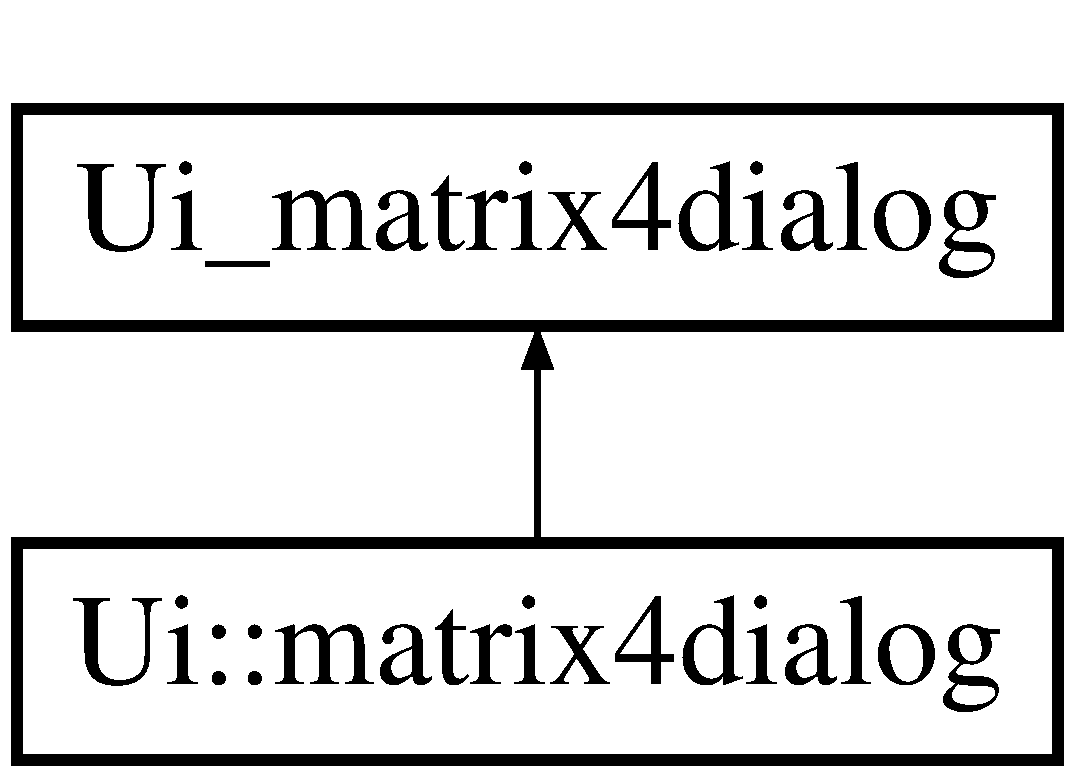
\includegraphics[height=2.000000cm]{class_ui__matrix4dialog}
\end{center}
\end{figure}
\subsection*{Public Member Functions}
\begin{DoxyCompactItemize}
\item 
\mbox{\Hypertarget{class_ui__matrix4dialog_aef219b6ca55919d404217da65f6d9f84}\label{class_ui__matrix4dialog_aef219b6ca55919d404217da65f6d9f84}} 
void {\bfseries setup\+Ui} (Q\+Dialog $\ast$\mbox{\hyperlink{classmatrix4dialog}{matrix4dialog}})
\item 
\mbox{\Hypertarget{class_ui__matrix4dialog_a0140e00a8003ec0682fad02b5422c32c}\label{class_ui__matrix4dialog_a0140e00a8003ec0682fad02b5422c32c}} 
void {\bfseries retranslate\+Ui} (Q\+Dialog $\ast$\mbox{\hyperlink{classmatrix4dialog}{matrix4dialog}})
\end{DoxyCompactItemize}
\subsection*{Public Attributes}
\begin{DoxyCompactItemize}
\item 
\mbox{\Hypertarget{class_ui__matrix4dialog_ae643e32c20b920b6ab7339075a79bd9d}\label{class_ui__matrix4dialog_ae643e32c20b920b6ab7339075a79bd9d}} 
Q\+Dialog\+Button\+Box $\ast$ {\bfseries button\+Box}
\item 
\mbox{\Hypertarget{class_ui__matrix4dialog_aa24b0549035d7da282a7a26c4076a08b}\label{class_ui__matrix4dialog_aa24b0549035d7da282a7a26c4076a08b}} 
Q\+Line\+Edit $\ast$ {\bfseries line\+Edit\+\_\+value2}
\item 
\mbox{\Hypertarget{class_ui__matrix4dialog_a0f6b83ac50476be0a50fe6581c58c9ec}\label{class_ui__matrix4dialog_a0f6b83ac50476be0a50fe6581c58c9ec}} 
Q\+Line\+Edit $\ast$ {\bfseries line\+Edit\+\_\+value4}
\item 
\mbox{\Hypertarget{class_ui__matrix4dialog_af76878b0323618ee71de96e1ff096e88}\label{class_ui__matrix4dialog_af76878b0323618ee71de96e1ff096e88}} 
Q\+Line\+Edit $\ast$ {\bfseries line\+Edit\+\_\+value1}
\item 
\mbox{\Hypertarget{class_ui__matrix4dialog_ab323365f4524b26c3aa16ca9cc2375c3}\label{class_ui__matrix4dialog_ab323365f4524b26c3aa16ca9cc2375c3}} 
Q\+Line\+Edit $\ast$ {\bfseries line\+Edit\+\_\+value3}
\item 
\mbox{\Hypertarget{class_ui__matrix4dialog_a251052fdd26c4f5d32480e10b296be69}\label{class_ui__matrix4dialog_a251052fdd26c4f5d32480e10b296be69}} 
Q\+Label $\ast$ {\bfseries label}
\item 
\mbox{\Hypertarget{class_ui__matrix4dialog_af1865005bfda4019dcf37b95b5c6e0d7}\label{class_ui__matrix4dialog_af1865005bfda4019dcf37b95b5c6e0d7}} 
Q\+Label $\ast$ {\bfseries label\+\_\+2}
\item 
\mbox{\Hypertarget{class_ui__matrix4dialog_a855424564cf682a5b813162db19932c7}\label{class_ui__matrix4dialog_a855424564cf682a5b813162db19932c7}} 
Q\+Label $\ast$ {\bfseries label\+\_\+3}
\item 
\mbox{\Hypertarget{class_ui__matrix4dialog_aaccd6a9185cebcd9bafe533642500165}\label{class_ui__matrix4dialog_aaccd6a9185cebcd9bafe533642500165}} 
Q\+Label $\ast$ {\bfseries label\+\_\+4}
\end{DoxyCompactItemize}


The documentation for this class was generated from the following file\+:\begin{DoxyCompactItemize}
\item 
/\+Users/lukehutton/\+One\+Drive -\/ University of Leeds/\+University/\+Computer Science/\+Internship/moebinv-\/gui/moebinv-\/gui-\/build/ui\+\_\+matrix4dialog.\+h\end{DoxyCompactItemize}

\hypertarget{class_ui__matrix8dialog}{}\section{Ui\+\_\+matrix8dialog Class Reference}
\label{class_ui__matrix8dialog}\index{Ui\+\_\+matrix8dialog@{Ui\+\_\+matrix8dialog}}
Inheritance diagram for Ui\+\_\+matrix8dialog\+:\begin{figure}[H]
\begin{center}
\leavevmode
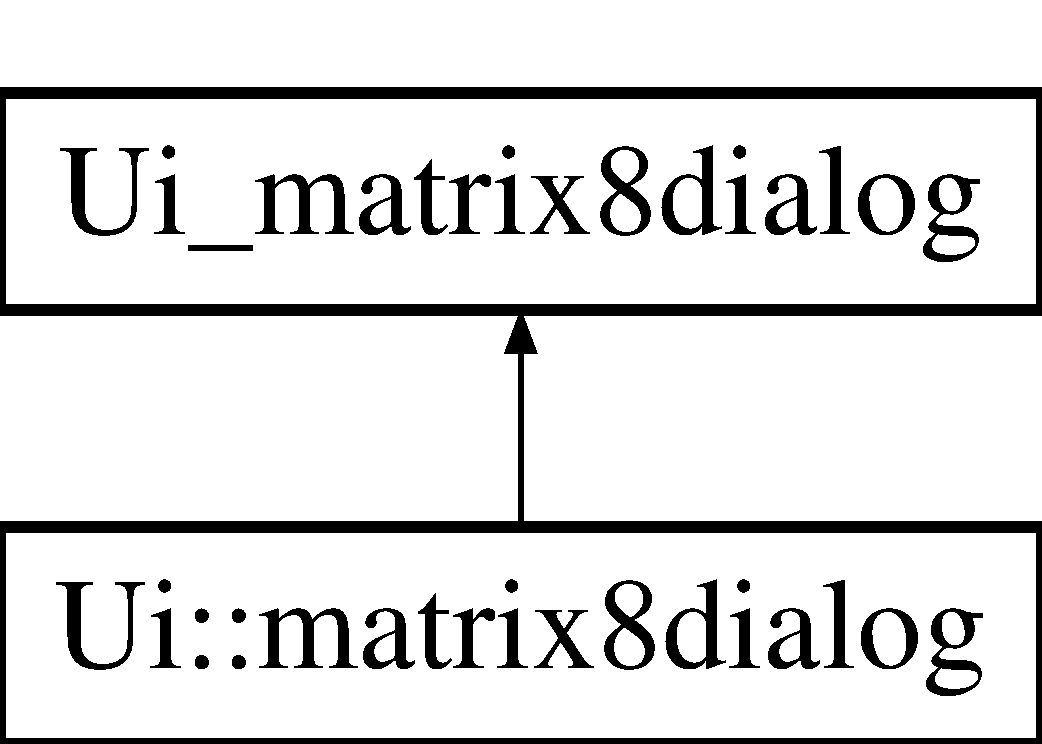
\includegraphics[height=2.000000cm]{class_ui__matrix8dialog}
\end{center}
\end{figure}
\subsection*{Public Member Functions}
\begin{DoxyCompactItemize}
\item 
\mbox{\Hypertarget{class_ui__matrix8dialog_a2b39e0a8327011911b0cd985a4d5697f}\label{class_ui__matrix8dialog_a2b39e0a8327011911b0cd985a4d5697f}} 
void {\bfseries setup\+Ui} (Q\+Dialog $\ast$\mbox{\hyperlink{classmatrix8dialog}{matrix8dialog}})
\item 
\mbox{\Hypertarget{class_ui__matrix8dialog_a1e76584117237b2839700411c6b1d748}\label{class_ui__matrix8dialog_a1e76584117237b2839700411c6b1d748}} 
void {\bfseries retranslate\+Ui} (Q\+Dialog $\ast$\mbox{\hyperlink{classmatrix8dialog}{matrix8dialog}})
\end{DoxyCompactItemize}
\subsection*{Public Attributes}
\begin{DoxyCompactItemize}
\item 
\mbox{\Hypertarget{class_ui__matrix8dialog_a05caf47b40e45d204c2bd9613a8d955a}\label{class_ui__matrix8dialog_a05caf47b40e45d204c2bd9613a8d955a}} 
Q\+Dialog\+Button\+Box $\ast$ {\bfseries button\+Box}
\item 
\mbox{\Hypertarget{class_ui__matrix8dialog_a73c18fd36dada64bae0c1dfdd4467699}\label{class_ui__matrix8dialog_a73c18fd36dada64bae0c1dfdd4467699}} 
Q\+Line\+Edit $\ast$ {\bfseries line\+Edit\+\_\+value2}
\item 
\mbox{\Hypertarget{class_ui__matrix8dialog_a34ab1fde638ea494cab0b6e8b49e339f}\label{class_ui__matrix8dialog_a34ab1fde638ea494cab0b6e8b49e339f}} 
Q\+Label $\ast$ {\bfseries label\+\_\+2}
\item 
\mbox{\Hypertarget{class_ui__matrix8dialog_a5898b8f9962f3ff9a19c4a801177306c}\label{class_ui__matrix8dialog_a5898b8f9962f3ff9a19c4a801177306c}} 
Q\+Line\+Edit $\ast$ {\bfseries line\+Edit\+\_\+value3}
\item 
\mbox{\Hypertarget{class_ui__matrix8dialog_ae19ba85fd7ddeb22e754a4eeb46aef24}\label{class_ui__matrix8dialog_ae19ba85fd7ddeb22e754a4eeb46aef24}} 
Q\+Label $\ast$ {\bfseries label}
\item 
\mbox{\Hypertarget{class_ui__matrix8dialog_a302027e9bca42c3d8709c82fa7249d9d}\label{class_ui__matrix8dialog_a302027e9bca42c3d8709c82fa7249d9d}} 
Q\+Label $\ast$ {\bfseries label\+\_\+4}
\item 
\mbox{\Hypertarget{class_ui__matrix8dialog_aef722cd4314ed9b4a9c91b5272138380}\label{class_ui__matrix8dialog_aef722cd4314ed9b4a9c91b5272138380}} 
Q\+Line\+Edit $\ast$ {\bfseries line\+Edit\+\_\+value4}
\item 
\mbox{\Hypertarget{class_ui__matrix8dialog_abb97b8de24dd00e5f7d6ad36c7bc009c}\label{class_ui__matrix8dialog_abb97b8de24dd00e5f7d6ad36c7bc009c}} 
Q\+Label $\ast$ {\bfseries label\+\_\+3}
\item 
\mbox{\Hypertarget{class_ui__matrix8dialog_a60c80910c009351097ddd66eb8e06253}\label{class_ui__matrix8dialog_a60c80910c009351097ddd66eb8e06253}} 
Q\+Line\+Edit $\ast$ {\bfseries line\+Edit\+\_\+value1}
\item 
\mbox{\Hypertarget{class_ui__matrix8dialog_ac7c6fa572253de8781d51b59ded2893a}\label{class_ui__matrix8dialog_ac7c6fa572253de8781d51b59ded2893a}} 
Q\+Label $\ast$ {\bfseries label\+\_\+5}
\item 
\mbox{\Hypertarget{class_ui__matrix8dialog_aa1a34788df19af7cb4318cd55506013c}\label{class_ui__matrix8dialog_aa1a34788df19af7cb4318cd55506013c}} 
Q\+Line\+Edit $\ast$ {\bfseries line\+Edit\+\_\+value8}
\item 
\mbox{\Hypertarget{class_ui__matrix8dialog_ab0d3ddc7637b2d04609af1aba005d22b}\label{class_ui__matrix8dialog_ab0d3ddc7637b2d04609af1aba005d22b}} 
Q\+Line\+Edit $\ast$ {\bfseries line\+Edit\+\_\+value7}
\item 
\mbox{\Hypertarget{class_ui__matrix8dialog_a6b9d474e8b60af43933806b4c2fb7055}\label{class_ui__matrix8dialog_a6b9d474e8b60af43933806b4c2fb7055}} 
Q\+Line\+Edit $\ast$ {\bfseries line\+Edit\+\_\+value5}
\item 
\mbox{\Hypertarget{class_ui__matrix8dialog_a3bde654266d91ad7ac339ddcda446cff}\label{class_ui__matrix8dialog_a3bde654266d91ad7ac339ddcda446cff}} 
Q\+Label $\ast$ {\bfseries label\+\_\+6}
\item 
\mbox{\Hypertarget{class_ui__matrix8dialog_a56e4ea75bd746b2aefc18a48512a6612}\label{class_ui__matrix8dialog_a56e4ea75bd746b2aefc18a48512a6612}} 
Q\+Label $\ast$ {\bfseries label\+\_\+7}
\item 
\mbox{\Hypertarget{class_ui__matrix8dialog_ac6160d0d4e2382df77d0c61e168d271d}\label{class_ui__matrix8dialog_ac6160d0d4e2382df77d0c61e168d271d}} 
Q\+Label $\ast$ {\bfseries label\+\_\+8}
\item 
\mbox{\Hypertarget{class_ui__matrix8dialog_af8ee00326ad344afc1fe571fcef389fd}\label{class_ui__matrix8dialog_af8ee00326ad344afc1fe571fcef389fd}} 
Q\+Line\+Edit $\ast$ {\bfseries line\+Edit\+\_\+value6}
\end{DoxyCompactItemize}


The documentation for this class was generated from the following file\+:\begin{DoxyCompactItemize}
\item 
/\+Users/lukehutton/\+One\+Drive -\/ University of Leeds/\+University/\+Computer Science/\+Internship/moebinv-\/gui/moebinv-\/gui-\/build/ui\+\_\+matrix8dialog.\+h\end{DoxyCompactItemize}

\hypertarget{class_ui__properties_dialog}{}\section{Ui\+\_\+properties\+Dialog Class Reference}
\label{class_ui__properties_dialog}\index{Ui\+\_\+properties\+Dialog@{Ui\+\_\+properties\+Dialog}}
Inheritance diagram for Ui\+\_\+properties\+Dialog\+:\begin{figure}[H]
\begin{center}
\leavevmode
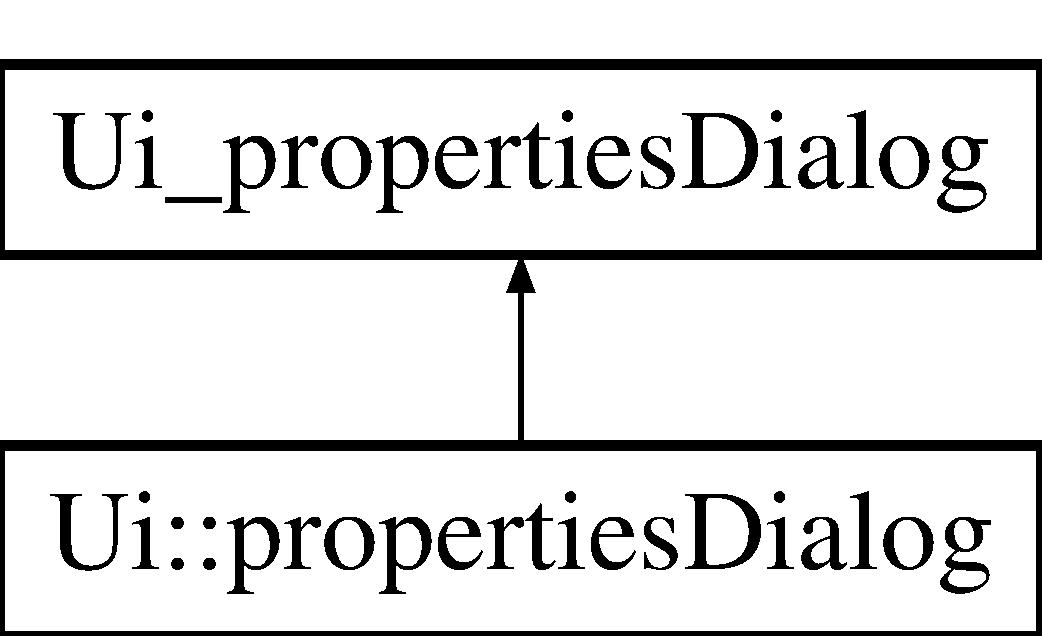
\includegraphics[height=2.000000cm]{class_ui__properties_dialog}
\end{center}
\end{figure}
\subsection*{Public Member Functions}
\begin{DoxyCompactItemize}
\item 
\mbox{\Hypertarget{class_ui__properties_dialog_a595c0d40bd7ea44fd12cb3d08cf5a9fb}\label{class_ui__properties_dialog_a595c0d40bd7ea44fd12cb3d08cf5a9fb}} 
void {\bfseries setup\+Ui} (Q\+Dialog $\ast$\mbox{\hyperlink{classproperties_dialog}{properties\+Dialog}})
\item 
\mbox{\Hypertarget{class_ui__properties_dialog_af4e86fdbed9259bb304605b4d414aecb}\label{class_ui__properties_dialog_af4e86fdbed9259bb304605b4d414aecb}} 
void {\bfseries retranslate\+Ui} (Q\+Dialog $\ast$\mbox{\hyperlink{classproperties_dialog}{properties\+Dialog}})
\end{DoxyCompactItemize}
\subsection*{Public Attributes}
\begin{DoxyCompactItemize}
\item 
\mbox{\Hypertarget{class_ui__properties_dialog_a98255232cbf624a7b15788f3db8c5240}\label{class_ui__properties_dialog_a98255232cbf624a7b15788f3db8c5240}} 
Q\+V\+Box\+Layout $\ast$ {\bfseries vertical\+Layout}
\item 
\mbox{\Hypertarget{class_ui__properties_dialog_aa4408a5d11640f91d67098cb57346179}\label{class_ui__properties_dialog_aa4408a5d11640f91d67098cb57346179}} 
Q\+Group\+Box $\ast$ {\bfseries group\+Box}
\item 
\mbox{\Hypertarget{class_ui__properties_dialog_af0b5bd40650126b92f06aed5c9c5ad4e}\label{class_ui__properties_dialog_af0b5bd40650126b92f06aed5c9c5ad4e}} 
Q\+V\+Box\+Layout $\ast$ {\bfseries vertical\+Layout\+\_\+2}
\item 
\mbox{\Hypertarget{class_ui__properties_dialog_abdd6eabecff7576fc26e0fcce1ec5578}\label{class_ui__properties_dialog_abdd6eabecff7576fc26e0fcce1ec5578}} 
Q\+Text\+Edit $\ast$ {\bfseries figure\+Description\+Text}
\item 
\mbox{\Hypertarget{class_ui__properties_dialog_a209e64b037cdee834e22e417a00b6d5c}\label{class_ui__properties_dialog_a209e64b037cdee834e22e417a00b6d5c}} 
Q\+Group\+Box $\ast$ {\bfseries group\+Box\+\_\+4}
\item 
\mbox{\Hypertarget{class_ui__properties_dialog_aba58a87c91131c941e91a80f6fe3f175}\label{class_ui__properties_dialog_aba58a87c91131c941e91a80f6fe3f175}} 
Q\+H\+Box\+Layout $\ast$ {\bfseries horizontal\+Layout\+\_\+2}
\item 
\mbox{\Hypertarget{class_ui__properties_dialog_a524ae1db7433b72d6689e6afbac4aa52}\label{class_ui__properties_dialog_a524ae1db7433b72d6689e6afbac4aa52}} 
Q\+Radio\+Button $\ast$ {\bfseries float\+Button}
\item 
\mbox{\Hypertarget{class_ui__properties_dialog_abd227707bd8310869b8fbe15d7ca9cfe}\label{class_ui__properties_dialog_abd227707bd8310869b8fbe15d7ca9cfe}} 
Q\+Radio\+Button $\ast$ {\bfseries exact\+Button}
\item 
\mbox{\Hypertarget{class_ui__properties_dialog_a8562fe5c8fd461c2fae10f6e00f856dc}\label{class_ui__properties_dialog_a8562fe5c8fd461c2fae10f6e00f856dc}} 
Q\+H\+Box\+Layout $\ast$ {\bfseries horizontal\+Layout}
\item 
\mbox{\Hypertarget{class_ui__properties_dialog_ae8127b03eb0c346ac3c25227410326e1}\label{class_ui__properties_dialog_ae8127b03eb0c346ac3c25227410326e1}} 
Q\+Group\+Box $\ast$ {\bfseries group\+Box\+\_\+2}
\item 
\mbox{\Hypertarget{class_ui__properties_dialog_a7c81843ddff27d18375e13cfed9bfac0}\label{class_ui__properties_dialog_a7c81843ddff27d18375e13cfed9bfac0}} 
Q\+V\+Box\+Layout $\ast$ {\bfseries vertical\+Layout\+\_\+3}
\item 
\mbox{\Hypertarget{class_ui__properties_dialog_a9b2b3e033a44d84db89f5bf0c7977a3e}\label{class_ui__properties_dialog_a9b2b3e033a44d84db89f5bf0c7977a3e}} 
Q\+Radio\+Button $\ast$ {\bfseries elliptic\+Point\+Button}
\item 
\mbox{\Hypertarget{class_ui__properties_dialog_a86f31864696a9f676ad3fee8a0ef4ad6}\label{class_ui__properties_dialog_a86f31864696a9f676ad3fee8a0ef4ad6}} 
Q\+Radio\+Button $\ast$ {\bfseries parabolic\+Point\+Button}
\item 
\mbox{\Hypertarget{class_ui__properties_dialog_ad4c33c681b44790fc4671f08d7b9fe2c}\label{class_ui__properties_dialog_ad4c33c681b44790fc4671f08d7b9fe2c}} 
Q\+Radio\+Button $\ast$ {\bfseries hyperbolic\+Point\+Button}
\item 
\mbox{\Hypertarget{class_ui__properties_dialog_a5a9872252c004e5c3665e0de8a331d06}\label{class_ui__properties_dialog_a5a9872252c004e5c3665e0de8a331d06}} 
Q\+Group\+Box $\ast$ {\bfseries group\+Box\+\_\+3}
\item 
\mbox{\Hypertarget{class_ui__properties_dialog_a73c069e1cd6743f2304c5a8ccf5b3de0}\label{class_ui__properties_dialog_a73c069e1cd6743f2304c5a8ccf5b3de0}} 
Q\+V\+Box\+Layout $\ast$ {\bfseries vertical\+Layout\+\_\+4}
\item 
\mbox{\Hypertarget{class_ui__properties_dialog_acc387e99d883c6337a06bf7c767a58c4}\label{class_ui__properties_dialog_acc387e99d883c6337a06bf7c767a58c4}} 
Q\+Radio\+Button $\ast$ {\bfseries elliptic\+Cycle\+Button}
\item 
\mbox{\Hypertarget{class_ui__properties_dialog_aa6488e9cda300c6fb580ff1103e6a3e3}\label{class_ui__properties_dialog_aa6488e9cda300c6fb580ff1103e6a3e3}} 
Q\+Radio\+Button $\ast$ {\bfseries parabolic\+Cycle\+Button}
\item 
\mbox{\Hypertarget{class_ui__properties_dialog_aeb4b1f6b0ff897d31e89dbe8689e223c}\label{class_ui__properties_dialog_aeb4b1f6b0ff897d31e89dbe8689e223c}} 
Q\+Radio\+Button $\ast$ {\bfseries hyperbolic\+Cycle\+Button}
\item 
\mbox{\Hypertarget{class_ui__properties_dialog_a7ef037d1f46fe6b15d6bd06be637cbf0}\label{class_ui__properties_dialog_a7ef037d1f46fe6b15d6bd06be637cbf0}} 
Q\+Spacer\+Item $\ast$ {\bfseries vertical\+Spacer}
\item 
\mbox{\Hypertarget{class_ui__properties_dialog_a1ccb0e1a0369f5ef66245528379f05a5}\label{class_ui__properties_dialog_a1ccb0e1a0369f5ef66245528379f05a5}} 
Q\+Dialog\+Button\+Box $\ast$ {\bfseries button\+Box}
\end{DoxyCompactItemize}


The documentation for this class was generated from the following file\+:\begin{DoxyCompactItemize}
\item 
/\+Users/lukehutton/\+One\+Drive -\/ University of Leeds/\+University/\+Computer Science/\+Internship/moebinv-\/gui/moebinv-\/gui-\/build/ui\+\_\+propertiesdialog.\+h\end{DoxyCompactItemize}

\hypertarget{class_ui__settings_dialog}{}\section{Ui\+\_\+settings\+Dialog Class Reference}
\label{class_ui__settings_dialog}\index{Ui\+\_\+settings\+Dialog@{Ui\+\_\+settings\+Dialog}}
Inheritance diagram for Ui\+\_\+settings\+Dialog\+:\begin{figure}[H]
\begin{center}
\leavevmode
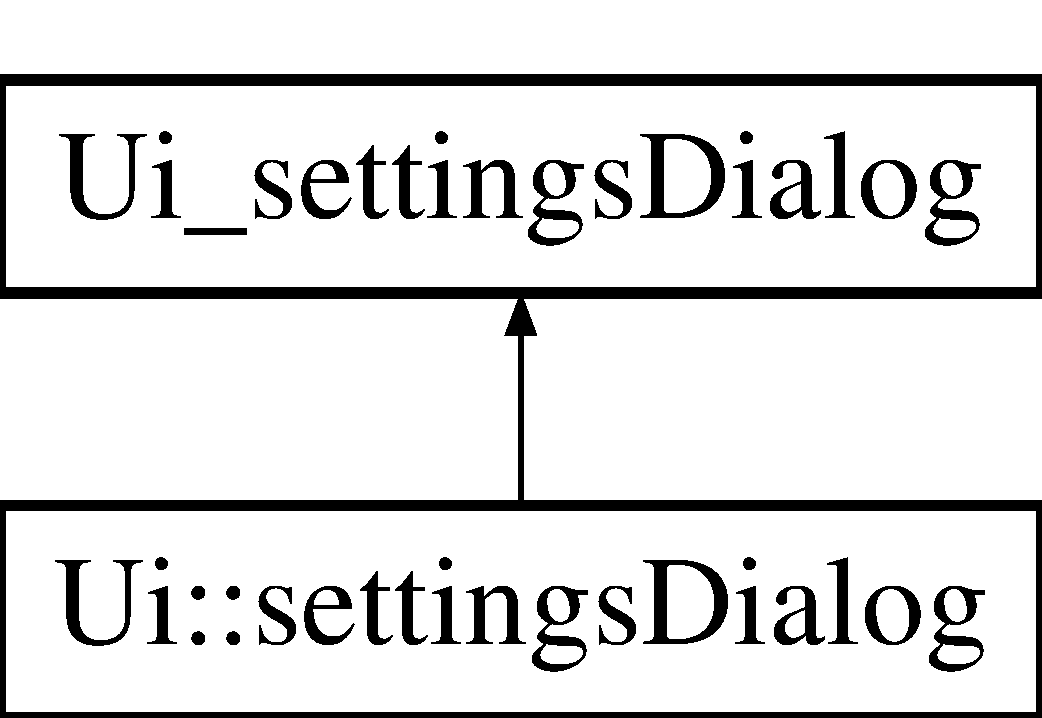
\includegraphics[height=2.000000cm]{class_ui__settings_dialog}
\end{center}
\end{figure}
\subsection*{Public Member Functions}
\begin{DoxyCompactItemize}
\item 
\mbox{\Hypertarget{class_ui__settings_dialog_af96d6b02d7d9762b18d968d8c8128f82}\label{class_ui__settings_dialog_af96d6b02d7d9762b18d968d8c8128f82}} 
void {\bfseries setup\+Ui} (Q\+Dialog $\ast$\mbox{\hyperlink{classsettings_dialog}{settings\+Dialog}})
\item 
\mbox{\Hypertarget{class_ui__settings_dialog_a41fc817d3b4a6103aee2ded4a8f5c273}\label{class_ui__settings_dialog_a41fc817d3b4a6103aee2ded4a8f5c273}} 
void {\bfseries retranslate\+Ui} (Q\+Dialog $\ast$\mbox{\hyperlink{classsettings_dialog}{settings\+Dialog}})
\end{DoxyCompactItemize}
\subsection*{Public Attributes}
\begin{DoxyCompactItemize}
\item 
\mbox{\Hypertarget{class_ui__settings_dialog_a41905fe1434ea89cee3595f6c860b5a6}\label{class_ui__settings_dialog_a41905fe1434ea89cee3595f6c860b5a6}} 
Q\+V\+Box\+Layout $\ast$ {\bfseries vertical\+Layout\+\_\+4}
\item 
\mbox{\Hypertarget{class_ui__settings_dialog_acc596f6a2cac5c3ecc2ce520a20c827a}\label{class_ui__settings_dialog_acc596f6a2cac5c3ecc2ce520a20c827a}} 
Q\+Tab\+Widget $\ast$ {\bfseries tab\+Widget}
\item 
\mbox{\Hypertarget{class_ui__settings_dialog_acf10507cd54902c83445442e3e09b738}\label{class_ui__settings_dialog_acf10507cd54902c83445442e3e09b738}} 
Q\+Widget $\ast$ {\bfseries tab}
\item 
\mbox{\Hypertarget{class_ui__settings_dialog_a3164e8026801dea9804a1354b78c38da}\label{class_ui__settings_dialog_a3164e8026801dea9804a1354b78c38da}} 
Q\+V\+Box\+Layout $\ast$ {\bfseries vertical\+Layout\+\_\+2}
\item 
\mbox{\Hypertarget{class_ui__settings_dialog_ad1d3781d92fe311f7b670e9c8f04ec6e}\label{class_ui__settings_dialog_ad1d3781d92fe311f7b670e9c8f04ec6e}} 
Q\+Group\+Box $\ast$ {\bfseries group\+Box}
\item 
\mbox{\Hypertarget{class_ui__settings_dialog_a2433db810a7ae0d57857076825e096a0}\label{class_ui__settings_dialog_a2433db810a7ae0d57857076825e096a0}} 
Q\+H\+Box\+Layout $\ast$ {\bfseries horizontal\+Layout}
\item 
\mbox{\Hypertarget{class_ui__settings_dialog_ab0faaf97c711d41d8919c92c3f268b1c}\label{class_ui__settings_dialog_ab0faaf97c711d41d8919c92c3f268b1c}} 
Q\+Radio\+Button $\ast$ {\bfseries automatic\+Naming}
\item 
\mbox{\Hypertarget{class_ui__settings_dialog_adbfba48f832ee2f84b61c7f9d236197e}\label{class_ui__settings_dialog_adbfba48f832ee2f84b61c7f9d236197e}} 
Q\+Radio\+Button $\ast$ {\bfseries manual\+Naming}
\item 
\mbox{\Hypertarget{class_ui__settings_dialog_aeedea3eec08a9525afec84e0bb18c5e6}\label{class_ui__settings_dialog_aeedea3eec08a9525afec84e0bb18c5e6}} 
Q\+Group\+Box $\ast$ {\bfseries group\+Box\+\_\+2}
\item 
\mbox{\Hypertarget{class_ui__settings_dialog_a5c11a50452e48905ceb877c0f143558a}\label{class_ui__settings_dialog_a5c11a50452e48905ceb877c0f143558a}} 
Q\+V\+Box\+Layout $\ast$ {\bfseries vertical\+Layout\+\_\+3}
\item 
\mbox{\Hypertarget{class_ui__settings_dialog_a3d632ee44f600bfda94dd22c8b865b2d}\label{class_ui__settings_dialog_a3d632ee44f600bfda94dd22c8b865b2d}} 
Q\+Double\+Spin\+Box $\ast$ {\bfseries double\+Spin\+Box}
\item 
\mbox{\Hypertarget{class_ui__settings_dialog_a3e8f7010593ce0a07d566c17dc5cd3e7}\label{class_ui__settings_dialog_a3e8f7010593ce0a07d566c17dc5cd3e7}} 
Q\+Group\+Box $\ast$ {\bfseries group\+Box\+\_\+6}
\item 
\mbox{\Hypertarget{class_ui__settings_dialog_a029c3789c703085c4f6677e7925292d6}\label{class_ui__settings_dialog_a029c3789c703085c4f6677e7925292d6}} 
Q\+H\+Box\+Layout $\ast$ {\bfseries horizontal\+Layout\+\_\+3}
\item 
\mbox{\Hypertarget{class_ui__settings_dialog_ae202f250dd6da958d0920b4665d1917f}\label{class_ui__settings_dialog_ae202f250dd6da958d0920b4665d1917f}} 
Q\+Line\+Edit $\ast$ {\bfseries default\+Path\+Line\+Edit}
\item 
\mbox{\Hypertarget{class_ui__settings_dialog_a9bcd42185b37bce81ab51a787ae6493b}\label{class_ui__settings_dialog_a9bcd42185b37bce81ab51a787ae6493b}} 
Q\+Push\+Button $\ast$ {\bfseries push\+Button\+\_\+4}
\item 
\mbox{\Hypertarget{class_ui__settings_dialog_aea78afbe2f62103d25386617107ba544}\label{class_ui__settings_dialog_aea78afbe2f62103d25386617107ba544}} 
Q\+Group\+Box $\ast$ {\bfseries group\+Box\+\_\+7}
\item 
\mbox{\Hypertarget{class_ui__settings_dialog_ad7c6cf95448da5fdbd25816a1b8cd631}\label{class_ui__settings_dialog_ad7c6cf95448da5fdbd25816a1b8cd631}} 
Q\+H\+Box\+Layout $\ast$ {\bfseries horizontal\+Layout\+\_\+2}
\item 
\mbox{\Hypertarget{class_ui__settings_dialog_a3954ad627be6db1470e4c958f4132526}\label{class_ui__settings_dialog_a3954ad627be6db1470e4c958f4132526}} 
Q\+Radio\+Button $\ast$ {\bfseries only\+Reals\+True}
\item 
\mbox{\Hypertarget{class_ui__settings_dialog_a24ff462fecd5f6a6c8372779b20d5042}\label{class_ui__settings_dialog_a24ff462fecd5f6a6c8372779b20d5042}} 
Q\+Radio\+Button $\ast$ {\bfseries only\+Reals\+False}
\item 
\mbox{\Hypertarget{class_ui__settings_dialog_a510fbc4798016d07406a498374867722}\label{class_ui__settings_dialog_a510fbc4798016d07406a498374867722}} 
Q\+Group\+Box $\ast$ {\bfseries group\+Box\+\_\+8}
\item 
\mbox{\Hypertarget{class_ui__settings_dialog_a4fe94889101443b99ba127a647d9fc43}\label{class_ui__settings_dialog_a4fe94889101443b99ba127a647d9fc43}} 
Q\+V\+Box\+Layout $\ast$ {\bfseries vertical\+Layout\+\_\+6}
\item 
\mbox{\Hypertarget{class_ui__settings_dialog_aa1039d8dae1b572300fa54f7c3e18646}\label{class_ui__settings_dialog_aa1039d8dae1b572300fa54f7c3e18646}} 
Q\+Spin\+Box $\ast$ {\bfseries spin\+Box}
\item 
\mbox{\Hypertarget{class_ui__settings_dialog_a7ef380f555a0a3e2e274000f6338c965}\label{class_ui__settings_dialog_a7ef380f555a0a3e2e274000f6338c965}} 
Q\+Spacer\+Item $\ast$ {\bfseries vertical\+Spacer}
\item 
\mbox{\Hypertarget{class_ui__settings_dialog_a64fe5c5093202932607b29e9af7c378b}\label{class_ui__settings_dialog_a64fe5c5093202932607b29e9af7c378b}} 
Q\+Widget $\ast$ {\bfseries tab\+\_\+2}
\item 
\mbox{\Hypertarget{class_ui__settings_dialog_ad02c41c8dcba75bcfe6a841fd87371fc}\label{class_ui__settings_dialog_ad02c41c8dcba75bcfe6a841fd87371fc}} 
Q\+V\+Box\+Layout $\ast$ {\bfseries vertical\+Layout}
\item 
\mbox{\Hypertarget{class_ui__settings_dialog_ab6039b08fe7033d8632ba959a1f9f458}\label{class_ui__settings_dialog_ab6039b08fe7033d8632ba959a1f9f458}} 
Q\+Group\+Box $\ast$ {\bfseries group\+Box\+\_\+3}
\item 
\mbox{\Hypertarget{class_ui__settings_dialog_a9cbb60155b2df0b006c2615493b136ee}\label{class_ui__settings_dialog_a9cbb60155b2df0b006c2615493b136ee}} 
Q\+Grid\+Layout $\ast$ {\bfseries grid\+Layout}
\item 
\mbox{\Hypertarget{class_ui__settings_dialog_add772572c6b6d5eeecd754a913b931be}\label{class_ui__settings_dialog_add772572c6b6d5eeecd754a913b931be}} 
Q\+Label $\ast$ {\bfseries label}
\item 
\mbox{\Hypertarget{class_ui__settings_dialog_ad3cf5fe1bdd892adf122893d92d3be22}\label{class_ui__settings_dialog_ad3cf5fe1bdd892adf122893d92d3be22}} 
Q\+Spacer\+Item $\ast$ {\bfseries horizontal\+Spacer}
\item 
\mbox{\Hypertarget{class_ui__settings_dialog_abb80c05c318bdf7b89da56bdd02974c4}\label{class_ui__settings_dialog_abb80c05c318bdf7b89da56bdd02974c4}} 
Q\+Push\+Button $\ast$ {\bfseries push\+Button\+\_\+2}
\item 
\mbox{\Hypertarget{class_ui__settings_dialog_aeffd642eb2c046e6c0ea941846bdb988}\label{class_ui__settings_dialog_aeffd642eb2c046e6c0ea941846bdb988}} 
Q\+Spacer\+Item $\ast$ {\bfseries horizontal\+Spacer\+\_\+2}
\item 
\mbox{\Hypertarget{class_ui__settings_dialog_ac591889922f52c0d47892ee9217d2fcd}\label{class_ui__settings_dialog_ac591889922f52c0d47892ee9217d2fcd}} 
Q\+Label $\ast$ {\bfseries label\+\_\+2}
\item 
\mbox{\Hypertarget{class_ui__settings_dialog_aeab6baefbf0bf0d9d3bd107130b80349}\label{class_ui__settings_dialog_aeab6baefbf0bf0d9d3bd107130b80349}} 
Q\+Label $\ast$ {\bfseries label\+\_\+3}
\item 
\mbox{\Hypertarget{class_ui__settings_dialog_ada86439f18c5657ac82583030dfd7604}\label{class_ui__settings_dialog_ada86439f18c5657ac82583030dfd7604}} 
Q\+Push\+Button $\ast$ {\bfseries push\+Button}
\item 
\mbox{\Hypertarget{class_ui__settings_dialog_a441acb931c49542379e5f97e215c860e}\label{class_ui__settings_dialog_a441acb931c49542379e5f97e215c860e}} 
Q\+Push\+Button $\ast$ {\bfseries push\+Button\+\_\+3}
\item 
\mbox{\Hypertarget{class_ui__settings_dialog_a58c2390d2c0ead93a2b360e4b3059b8a}\label{class_ui__settings_dialog_a58c2390d2c0ead93a2b360e4b3059b8a}} 
Q\+Spacer\+Item $\ast$ {\bfseries horizontal\+Spacer\+\_\+3}
\item 
\mbox{\Hypertarget{class_ui__settings_dialog_a833c48e589e0b65f6314673f5f9e04a9}\label{class_ui__settings_dialog_a833c48e589e0b65f6314673f5f9e04a9}} 
Q\+Group\+Box $\ast$ {\bfseries group\+Box\+\_\+4}
\item 
\mbox{\Hypertarget{class_ui__settings_dialog_a8747cf83ce4127dab0cb1e7f7a1fd8d8}\label{class_ui__settings_dialog_a8747cf83ce4127dab0cb1e7f7a1fd8d8}} 
Q\+Grid\+Layout $\ast$ {\bfseries grid\+Layout\+\_\+2}
\item 
\mbox{\Hypertarget{class_ui__settings_dialog_a864626ed59d209e907310a99e6441420}\label{class_ui__settings_dialog_a864626ed59d209e907310a99e6441420}} 
Q\+Label $\ast$ {\bfseries label\+\_\+4}
\item 
\mbox{\Hypertarget{class_ui__settings_dialog_aa64ac7eca46c9267f8e454b072071a07}\label{class_ui__settings_dialog_aa64ac7eca46c9267f8e454b072071a07}} 
Q\+Spacer\+Item $\ast$ {\bfseries horizontal\+Spacer\+\_\+4}
\item 
\mbox{\Hypertarget{class_ui__settings_dialog_af4beec48c7690a2c9b6d57904f87d0c5}\label{class_ui__settings_dialog_af4beec48c7690a2c9b6d57904f87d0c5}} 
Q\+Combo\+Box $\ast$ {\bfseries combo\+Box}
\item 
\mbox{\Hypertarget{class_ui__settings_dialog_ab041c5c10a03d19c9cc5fe7d69012e8c}\label{class_ui__settings_dialog_ab041c5c10a03d19c9cc5fe7d69012e8c}} 
Q\+Label $\ast$ {\bfseries label\+\_\+5}
\item 
\mbox{\Hypertarget{class_ui__settings_dialog_affdd0804285454c334853dd702f0f4c2}\label{class_ui__settings_dialog_affdd0804285454c334853dd702f0f4c2}} 
Q\+Double\+Spin\+Box $\ast$ {\bfseries double\+Spin\+Box\+\_\+2}
\item 
\mbox{\Hypertarget{class_ui__settings_dialog_affd52a1b02f018dbeb5261a37f7aa9fb}\label{class_ui__settings_dialog_affd52a1b02f018dbeb5261a37f7aa9fb}} 
Q\+Spacer\+Item $\ast$ {\bfseries horizontal\+Spacer\+\_\+5}
\item 
\mbox{\Hypertarget{class_ui__settings_dialog_a766fad3cfaf98dde8ae45ce9392e250a}\label{class_ui__settings_dialog_a766fad3cfaf98dde8ae45ce9392e250a}} 
Q\+Spacer\+Item $\ast$ {\bfseries vertical\+Spacer\+\_\+2}
\item 
\mbox{\Hypertarget{class_ui__settings_dialog_a9fd9aea95caaf8c0f62efbb46711d137}\label{class_ui__settings_dialog_a9fd9aea95caaf8c0f62efbb46711d137}} 
Q\+Dialog\+Button\+Box $\ast$ {\bfseries button\+Box}
\end{DoxyCompactItemize}


The documentation for this class was generated from the following file\+:\begin{DoxyCompactItemize}
\item 
/\+Users/lukehutton/\+One\+Drive -\/ University of Leeds/\+University/\+Computer Science/\+Internship/moebinv-\/gui/moebinv-\/gui-\/build/ui\+\_\+settingsdialog.\+h\end{DoxyCompactItemize}

\hypertarget{classview}{}\section{view Class Reference}
\label{classview}\index{view@{view}}
Inheritance diagram for view\+:\begin{figure}[H]
\begin{center}
\leavevmode
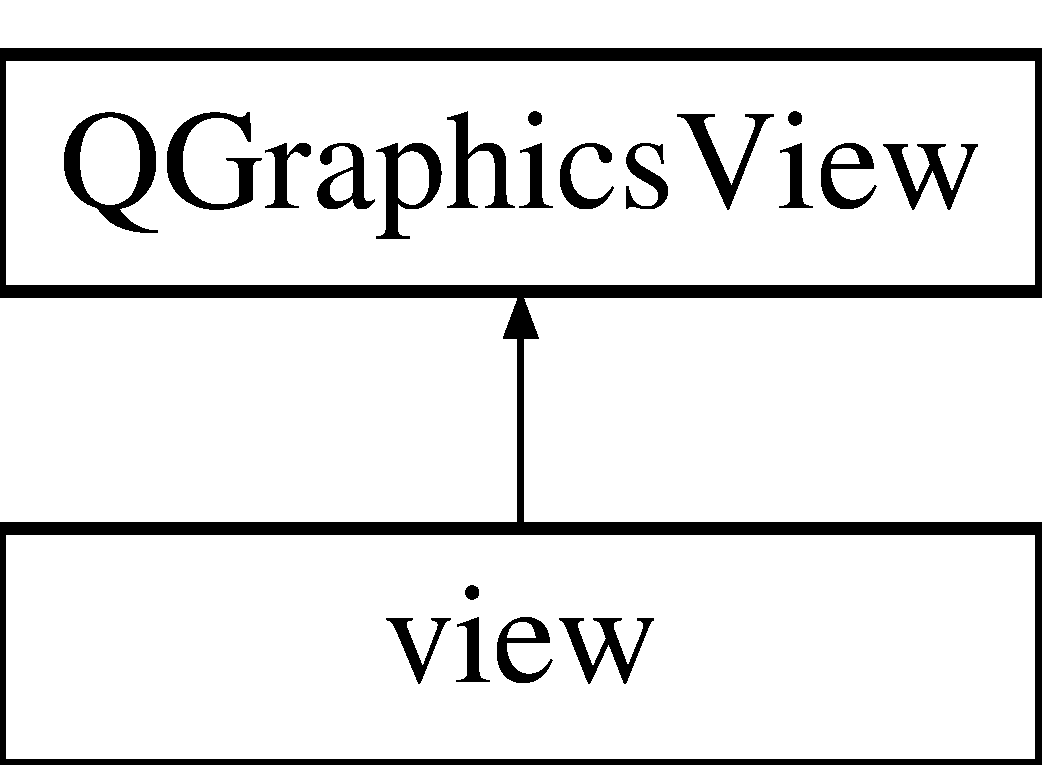
\includegraphics[height=2.000000cm]{classview}
\end{center}
\end{figure}
\subsection*{Public Slots}
\begin{DoxyCompactItemize}
\item 
void \mbox{\hyperlink{classview_a7fff213d7f38eeb2c8943609264fa518}{recenter\+View}} ()
\begin{DoxyCompactList}\small\item\em \mbox{\hyperlink{classview_a7fff213d7f38eeb2c8943609264fa518}{view\+::recenter\+View}} Recenter the view \end{DoxyCompactList}\item 
void \mbox{\hyperlink{classview_ab1d79ebdee961d5ec07ed11f461158a5}{mouse\+Stopped}} ()
\begin{DoxyCompactList}\small\item\em \mbox{\hyperlink{classview_ab1d79ebdee961d5ec07ed11f461158a5}{view\+::mouse\+Stopped}} \end{DoxyCompactList}\item 
\mbox{\Hypertarget{classview_a3eedee38e4dfa3d2fa7f30f52c36438b}\label{classview_a3eedee38e4dfa3d2fa7f30f52c36438b}} 
void {\bfseries set\+Background\+Colour} (Q\+Color colour)
\end{DoxyCompactItemize}
\subsection*{Signals}
\begin{DoxyCompactItemize}
\item 
\mbox{\Hypertarget{classview_ab0e83744c774f7cb76dbfc8ce12c4186}\label{classview_ab0e83744c774f7cb76dbfc8ce12c4186}} 
void {\bfseries highlight\+Closest\+Cycle} (Q\+PointF \mbox{\hyperlink{classpoint}{point}})
\end{DoxyCompactItemize}
\subsection*{Public Member Functions}
\begin{DoxyCompactItemize}
\item 
\mbox{\hyperlink{classview_a5b500c7ca4c4631a614445bcf8c06ed8}{view}} (Q\+Widget $\ast$parent=nullptr)
\begin{DoxyCompactList}\small\item\em \mbox{\hyperlink{classview_a5b500c7ca4c4631a614445bcf8c06ed8}{view\+::view}} Construct a new view. \end{DoxyCompactList}\item 
bool \mbox{\hyperlink{classview_aea81f104e17ad13b12d66dabc82b2df0}{get\+Panning\+Enabled}} ()
\begin{DoxyCompactList}\small\item\em \mbox{\hyperlink{classview_aea81f104e17ad13b12d66dabc82b2df0}{view\+::get\+Panning\+Enabled}} getter for panning enabled. \end{DoxyCompactList}\item 
void \mbox{\hyperlink{classview_a78e6621aad0346c49fc9d9e0e4f268f5}{set\+Panning\+Enabled}} (const bool \&value)
\begin{DoxyCompactList}\small\item\em \mbox{\hyperlink{classview_a78e6621aad0346c49fc9d9e0e4f268f5}{view\+::set\+Panning\+Enabled}} setter for panning enabled. \end{DoxyCompactList}\item 
Q\+Pointer$<$ \mbox{\hyperlink{classgraphic_cycle}{graphic\+Cycle}} $>$ \mbox{\hyperlink{classview_aa0b6bfa057ab5c4d8f3bd60557622533}{get\+Current\+Highlighted\+Cycle}} ()
\begin{DoxyCompactList}\small\item\em \mbox{\hyperlink{classview_aa0b6bfa057ab5c4d8f3bd60557622533}{view\+::get\+Current\+Highlighted\+Cycle}} getter for current\+Highlighted\+Cycle. \end{DoxyCompactList}\item 
void \mbox{\hyperlink{classview_a69ba93a57967891ba91517b9fd50e369}{set\+Current\+Highlighted\+Cycle}} (const Q\+Pointer$<$ \mbox{\hyperlink{classgraphic_cycle}{graphic\+Cycle}} $>$ cycle)
\begin{DoxyCompactList}\small\item\em \mbox{\hyperlink{classview_a69ba93a57967891ba91517b9fd50e369}{view\+::set\+Current\+Highlighted\+Cycle}} setter for currently highlighted cycle. \end{DoxyCompactList}\item 
void \mbox{\hyperlink{classview_a7d18b10e6f370227079c552df12d4c02}{wheel\+Event}} (Q\+Wheel\+Event $\ast$event)
\begin{DoxyCompactList}\small\item\em \mbox{\hyperlink{classview_a7d18b10e6f370227079c552df12d4c02}{view\+::wheel\+Event}} Implements zooming on scroll wheel. \end{DoxyCompactList}\item 
void \mbox{\hyperlink{classview_a7813d1b3e94e3c4db1ec0fa9143a1eca}{mouse\+Press\+Event}} (Q\+Mouse\+Event $\ast$event)
\begin{DoxyCompactList}\small\item\em \mbox{\hyperlink{classview_a7813d1b3e94e3c4db1ec0fa9143a1eca}{view\+::mouse\+Press\+Event}} handle panning on mouse press. \end{DoxyCompactList}\item 
void \mbox{\hyperlink{classview_a165a6cba84a12fc10fbf4c6fee73df73}{mouse\+Move\+Event}} (Q\+Mouse\+Event $\ast$event)
\begin{DoxyCompactList}\small\item\em \mbox{\hyperlink{classview_a165a6cba84a12fc10fbf4c6fee73df73}{view\+::mouse\+Move\+Event}} \end{DoxyCompactList}\item 
void \mbox{\hyperlink{classview_a57902641e912fe7549e04cc6a360d60c}{mouse\+Release\+Event}} (Q\+Mouse\+Event $\ast$event)
\begin{DoxyCompactList}\small\item\em \mbox{\hyperlink{classview_a57902641e912fe7549e04cc6a360d60c}{view\+::mouse\+Release\+Event}} mouse release event on view. \end{DoxyCompactList}\item 
void \mbox{\hyperlink{classview_af0f530013cb69c332de83d47d75a8fb0}{zoom\+In}} ()
\begin{DoxyCompactList}\small\item\em \mbox{\hyperlink{classview_af0f530013cb69c332de83d47d75a8fb0}{view\+::zoom\+In}} \end{DoxyCompactList}\item 
void \mbox{\hyperlink{classview_a497e42c804c9937d94b373d53e163f1b}{zoom\+Out}} ()
\begin{DoxyCompactList}\small\item\em \mbox{\hyperlink{classview_a497e42c804c9937d94b373d53e163f1b}{view\+::zoom\+Out}} \end{DoxyCompactList}\end{DoxyCompactItemize}
\subsection*{Public Attributes}
\begin{DoxyCompactItemize}
\item 
\mbox{\Hypertarget{classview_ae841c1e593aa326d706d2a52fe6275ba}\label{classview_ae841c1e593aa326d706d2a52fe6275ba}} 
double {\bfseries relative\+Scale\+Factor}
\end{DoxyCompactItemize}


\subsection{Constructor \& Destructor Documentation}
\mbox{\Hypertarget{classview_a5b500c7ca4c4631a614445bcf8c06ed8}\label{classview_a5b500c7ca4c4631a614445bcf8c06ed8}} 
\index{view@{view}!view@{view}}
\index{view@{view}!view@{view}}
\subsubsection{\texorpdfstring{view()}{view()}}
{\footnotesize\ttfamily view\+::view (\begin{DoxyParamCaption}\item[{Q\+Widget $\ast$}]{parent = {\ttfamily nullptr} }\end{DoxyParamCaption})\hspace{0.3cm}{\ttfamily [explicit]}}



\mbox{\hyperlink{classview_a5b500c7ca4c4631a614445bcf8c06ed8}{view\+::view}} Construct a new view. 


\begin{DoxyParams}{Parameters}
{\em parent} & parent object to the view.\\
\hline
\end{DoxyParams}
Construct a new view applying any settings. 

\subsection{Member Function Documentation}
\mbox{\Hypertarget{classview_aa0b6bfa057ab5c4d8f3bd60557622533}\label{classview_aa0b6bfa057ab5c4d8f3bd60557622533}} 
\index{view@{view}!get\+Current\+Highlighted\+Cycle@{get\+Current\+Highlighted\+Cycle}}
\index{get\+Current\+Highlighted\+Cycle@{get\+Current\+Highlighted\+Cycle}!view@{view}}
\subsubsection{\texorpdfstring{get\+Current\+Highlighted\+Cycle()}{getCurrentHighlightedCycle()}}
{\footnotesize\ttfamily Q\+Pointer$<$ \mbox{\hyperlink{classgraphic_cycle}{graphic\+Cycle}} $>$ view\+::get\+Current\+Highlighted\+Cycle (\begin{DoxyParamCaption}{ }\end{DoxyParamCaption})}



\mbox{\hyperlink{classview_aa0b6bfa057ab5c4d8f3bd60557622533}{view\+::get\+Current\+Highlighted\+Cycle}} getter for current\+Highlighted\+Cycle. 

\begin{DoxyReturn}{Returns}
\mbox{\hyperlink{classgraphic_cycle}{graphic\+Cycle}} 
\end{DoxyReturn}
\mbox{\Hypertarget{classview_aea81f104e17ad13b12d66dabc82b2df0}\label{classview_aea81f104e17ad13b12d66dabc82b2df0}} 
\index{view@{view}!get\+Panning\+Enabled@{get\+Panning\+Enabled}}
\index{get\+Panning\+Enabled@{get\+Panning\+Enabled}!view@{view}}
\subsubsection{\texorpdfstring{get\+Panning\+Enabled()}{getPanningEnabled()}}
{\footnotesize\ttfamily bool view\+::get\+Panning\+Enabled (\begin{DoxyParamCaption}{ }\end{DoxyParamCaption})}



\mbox{\hyperlink{classview_aea81f104e17ad13b12d66dabc82b2df0}{view\+::get\+Panning\+Enabled}} getter for panning enabled. 

\begin{DoxyReturn}{Returns}
bool 
\end{DoxyReturn}
\mbox{\Hypertarget{classview_a165a6cba84a12fc10fbf4c6fee73df73}\label{classview_a165a6cba84a12fc10fbf4c6fee73df73}} 
\index{view@{view}!mouse\+Move\+Event@{mouse\+Move\+Event}}
\index{mouse\+Move\+Event@{mouse\+Move\+Event}!view@{view}}
\subsubsection{\texorpdfstring{mouse\+Move\+Event()}{mouseMoveEvent()}}
{\footnotesize\ttfamily void view\+::mouse\+Move\+Event (\begin{DoxyParamCaption}\item[{Q\+Mouse\+Event $\ast$}]{event }\end{DoxyParamCaption})}



\mbox{\hyperlink{classview_a165a6cba84a12fc10fbf4c6fee73df73}{view\+::mouse\+Move\+Event}} 


\begin{DoxyParams}{Parameters}
{\em event} & Reimplemented event that is triggered when the mouse moves on the view. This allows panning to take place along with detecting when the mouse has stopped. \\
\hline
\end{DoxyParams}
\mbox{\Hypertarget{classview_a7813d1b3e94e3c4db1ec0fa9143a1eca}\label{classview_a7813d1b3e94e3c4db1ec0fa9143a1eca}} 
\index{view@{view}!mouse\+Press\+Event@{mouse\+Press\+Event}}
\index{mouse\+Press\+Event@{mouse\+Press\+Event}!view@{view}}
\subsubsection{\texorpdfstring{mouse\+Press\+Event()}{mousePressEvent()}}
{\footnotesize\ttfamily void view\+::mouse\+Press\+Event (\begin{DoxyParamCaption}\item[{Q\+Mouse\+Event $\ast$}]{event }\end{DoxyParamCaption})}



\mbox{\hyperlink{classview_a7813d1b3e94e3c4db1ec0fa9143a1eca}{view\+::mouse\+Press\+Event}} handle panning on mouse press. 


\begin{DoxyParams}{Parameters}
{\em event} & mouse event.\\
\hline
\end{DoxyParams}
Checks to see if the view needs panning on a mouse press. \mbox{\Hypertarget{classview_a57902641e912fe7549e04cc6a360d60c}\label{classview_a57902641e912fe7549e04cc6a360d60c}} 
\index{view@{view}!mouse\+Release\+Event@{mouse\+Release\+Event}}
\index{mouse\+Release\+Event@{mouse\+Release\+Event}!view@{view}}
\subsubsection{\texorpdfstring{mouse\+Release\+Event()}{mouseReleaseEvent()}}
{\footnotesize\ttfamily void view\+::mouse\+Release\+Event (\begin{DoxyParamCaption}\item[{Q\+Mouse\+Event $\ast$}]{event }\end{DoxyParamCaption})}



\mbox{\hyperlink{classview_a57902641e912fe7549e04cc6a360d60c}{view\+::mouse\+Release\+Event}} mouse release event on view. 


\begin{DoxyParams}{Parameters}
{\em event} & mouse event.\\
\hline
\end{DoxyParams}
Triggered when the mouse is released from the view. This function reimplements the existing function adding panning to it. \mbox{\Hypertarget{classview_ab1d79ebdee961d5ec07ed11f461158a5}\label{classview_ab1d79ebdee961d5ec07ed11f461158a5}} 
\index{view@{view}!mouse\+Stopped@{mouse\+Stopped}}
\index{mouse\+Stopped@{mouse\+Stopped}!view@{view}}
\subsubsection{\texorpdfstring{mouse\+Stopped}{mouseStopped}}
{\footnotesize\ttfamily void view\+::mouse\+Stopped (\begin{DoxyParamCaption}{ }\end{DoxyParamCaption})\hspace{0.3cm}{\ttfamily [slot]}}



\mbox{\hyperlink{classview_ab1d79ebdee961d5ec07ed11f461158a5}{view\+::mouse\+Stopped}} 

Slot that is triggered when the mouse has stopped moving. This slot then emits a signal to find the closest cycle to the current mouse position. \mbox{\Hypertarget{classview_a7fff213d7f38eeb2c8943609264fa518}\label{classview_a7fff213d7f38eeb2c8943609264fa518}} 
\index{view@{view}!recenter\+View@{recenter\+View}}
\index{recenter\+View@{recenter\+View}!view@{view}}
\subsubsection{\texorpdfstring{recenter\+View}{recenterView}}
{\footnotesize\ttfamily void view\+::recenter\+View (\begin{DoxyParamCaption}{ }\end{DoxyParamCaption})\hspace{0.3cm}{\ttfamily [slot]}}



\mbox{\hyperlink{classview_a7fff213d7f38eeb2c8943609264fa518}{view\+::recenter\+View}} Recenter the view 

Recenter the view to the default point (0, 0). \mbox{\Hypertarget{classview_a69ba93a57967891ba91517b9fd50e369}\label{classview_a69ba93a57967891ba91517b9fd50e369}} 
\index{view@{view}!set\+Current\+Highlighted\+Cycle@{set\+Current\+Highlighted\+Cycle}}
\index{set\+Current\+Highlighted\+Cycle@{set\+Current\+Highlighted\+Cycle}!view@{view}}
\subsubsection{\texorpdfstring{set\+Current\+Highlighted\+Cycle()}{setCurrentHighlightedCycle()}}
{\footnotesize\ttfamily void view\+::set\+Current\+Highlighted\+Cycle (\begin{DoxyParamCaption}\item[{const Q\+Pointer$<$ \mbox{\hyperlink{classgraphic_cycle}{graphic\+Cycle}} $>$}]{cycle }\end{DoxyParamCaption})}



\mbox{\hyperlink{classview_a69ba93a57967891ba91517b9fd50e369}{view\+::set\+Current\+Highlighted\+Cycle}} setter for currently highlighted cycle. 


\begin{DoxyParams}{Parameters}
{\em cycle} & \\
\hline
\end{DoxyParams}
\mbox{\Hypertarget{classview_a78e6621aad0346c49fc9d9e0e4f268f5}\label{classview_a78e6621aad0346c49fc9d9e0e4f268f5}} 
\index{view@{view}!set\+Panning\+Enabled@{set\+Panning\+Enabled}}
\index{set\+Panning\+Enabled@{set\+Panning\+Enabled}!view@{view}}
\subsubsection{\texorpdfstring{set\+Panning\+Enabled()}{setPanningEnabled()}}
{\footnotesize\ttfamily void view\+::set\+Panning\+Enabled (\begin{DoxyParamCaption}\item[{const bool \&}]{value }\end{DoxyParamCaption})}



\mbox{\hyperlink{classview_a78e6621aad0346c49fc9d9e0e4f268f5}{view\+::set\+Panning\+Enabled}} setter for panning enabled. 


\begin{DoxyParams}{Parameters}
{\em value} & \\
\hline
\end{DoxyParams}
\mbox{\Hypertarget{classview_a7d18b10e6f370227079c552df12d4c02}\label{classview_a7d18b10e6f370227079c552df12d4c02}} 
\index{view@{view}!wheel\+Event@{wheel\+Event}}
\index{wheel\+Event@{wheel\+Event}!view@{view}}
\subsubsection{\texorpdfstring{wheel\+Event()}{wheelEvent()}}
{\footnotesize\ttfamily void view\+::wheel\+Event (\begin{DoxyParamCaption}\item[{Q\+Wheel\+Event $\ast$}]{event }\end{DoxyParamCaption})}



\mbox{\hyperlink{classview_a7d18b10e6f370227079c552df12d4c02}{view\+::wheel\+Event}} Implements zooming on scroll wheel. 


\begin{DoxyParams}{Parameters}
{\em event} & Mouse wheel event.\\
\hline
\end{DoxyParams}
When the scroll wheel is used the view will either zoom in or out depending on the scroll wheel direction. \mbox{\Hypertarget{classview_af0f530013cb69c332de83d47d75a8fb0}\label{classview_af0f530013cb69c332de83d47d75a8fb0}} 
\index{view@{view}!zoom\+In@{zoom\+In}}
\index{zoom\+In@{zoom\+In}!view@{view}}
\subsubsection{\texorpdfstring{zoom\+In()}{zoomIn()}}
{\footnotesize\ttfamily void view\+::zoom\+In (\begin{DoxyParamCaption}{ }\end{DoxyParamCaption})}



\mbox{\hyperlink{classview_af0f530013cb69c332de83d47d75a8fb0}{view\+::zoom\+In}} 

Zoom in by a constant factor. \mbox{\Hypertarget{classview_a497e42c804c9937d94b373d53e163f1b}\label{classview_a497e42c804c9937d94b373d53e163f1b}} 
\index{view@{view}!zoom\+Out@{zoom\+Out}}
\index{zoom\+Out@{zoom\+Out}!view@{view}}
\subsubsection{\texorpdfstring{zoom\+Out()}{zoomOut()}}
{\footnotesize\ttfamily void view\+::zoom\+Out (\begin{DoxyParamCaption}{ }\end{DoxyParamCaption})}



\mbox{\hyperlink{classview_a497e42c804c9937d94b373d53e163f1b}{view\+::zoom\+Out}} 

Zoom out by a constant factor. 

The documentation for this class was generated from the following files\+:\begin{DoxyCompactItemize}
\item 
/\+Users/lukehutton/\+One\+Drive -\/ University of Leeds/\+University/\+Computer Science/\+Internship/moebinv-\/gui/include/view.\+h\item 
/\+Users/lukehutton/\+One\+Drive -\/ University of Leeds/\+University/\+Computer Science/\+Internship/moebinv-\/gui/moebinv-\/gui-\/build/moc\+\_\+view.\+cpp\item 
/\+Users/lukehutton/\+One\+Drive -\/ University of Leeds/\+University/\+Computer Science/\+Internship/moebinv-\/gui/src/view.\+cpp\end{DoxyCompactItemize}

\hypertarget{classvis}{}\section{vis Class Reference}
\label{classvis}\index{vis@{vis}}


{\ttfamily \#include $<$vis.\+h$>$}

Inheritance diagram for vis\+:\begin{figure}[H]
\begin{center}
\leavevmode
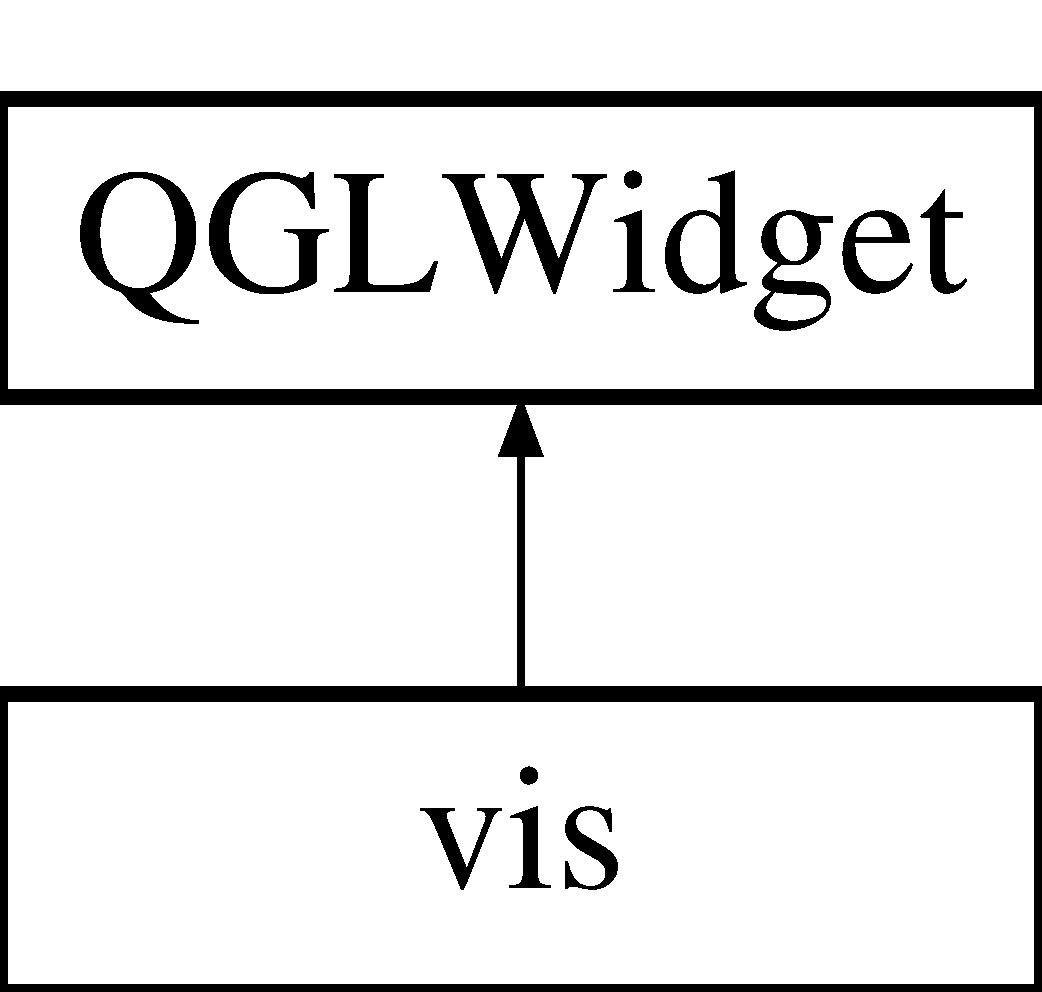
\includegraphics[height=2.000000cm]{classvis}
\end{center}
\end{figure}
\subsection*{Public Slots}
\begin{DoxyCompactItemize}
\item 
void \mbox{\hyperlink{classvis_a2338a54dfa9091ea6b050b814dc2b679}{set\+Col\+Slot}} (int col\+ID)
\item 
void \mbox{\hyperlink{classvis_ad217326086a9f0cfc1e35df9c7ccf9c0}{col\+Change\+Slot}} ()
\item 
void \mbox{\hyperlink{classvis_aa7568cc4804a9f945f54a4933ced67d0}{trans\+Slider\+Changed}} (int val)
\item 
void \mbox{\hyperlink{classvis_af2c43f4aaebe6ee5047e8eb9e9e8eedd}{trans\+Change\+Slot}} ()
\item 
void \mbox{\hyperlink{classvis_a192e67455047ca991fb29fbd4074c11d}{print\+Intersection\+Slot}} (int id)
\item 
void \mbox{\hyperlink{classvis_afd17774826a24e88c4f2eae14d85c7b4}{update\+Draw\+List}} ()
\item 
void \mbox{\hyperlink{classvis_af09e2926e8e8dfa0eca3d6b2f3946fdd}{print\+All\+Intersections}} ()
\item 
void \mbox{\hyperlink{classvis_aca0a94b8f2256122fc6e004a4d7de6e6}{draw\+All\+Intersections}} ()
\item 
void \mbox{\hyperlink{classvis_a09be90ab62dec1dcf2a72690d254acfb}{create\+Slide\+Dialog}} ()
\item 
void \mbox{\hyperlink{classvis_ae8441d597e876882029ee13b16aa4cc2}{set\+Slideshow}} ()
\item 
void \mbox{\hyperlink{classvis_aac05bc47936f37805e95dc251fd70035}{key\+Change}} (Q\+String key)
\item 
void \mbox{\hyperlink{classvis_a01552b5b750d2c56980b62dc1bc3dac9}{trans\+Change}} (Q\+String trans)
\item 
void \mbox{\hyperlink{classvis_aacae1519b8fc0799f9d3676bd35ab957}{group\+Change}} (Q\+String group)
\item 
void \mbox{\hyperlink{classvis_aa44c7eaf89bd4bc5dbcd75d4e2458ec7}{take\+Screenshot}} ()
\item 
int \mbox{\hyperlink{classvis_a2886cfbc9070b5622347b1c6c87dfe18}{file\+Loader}} ()
\end{DoxyCompactItemize}
\subsection*{Public Member Functions}
\begin{DoxyCompactItemize}
\item 
\mbox{\hyperlink{classvis_a996ee5697c4a48f0c9ae5743449fc69d}{vis}} (Q\+Widget $\ast$parent)
\begin{DoxyCompactList}\small\item\em class definition for 3d elliptic non-\/Euclidean visualisation tool. \end{DoxyCompactList}\item 
vector$<$ \mbox{\hyperlink{struct_point}{Point}} $>$ \mbox{\hyperlink{classvis_a9953ea49c09b9acec704d8175cb7865e}{make\+Sphere\+Points}} (int n\+Points)
\item 
vector$<$ \mbox{\hyperlink{struct_point}{Point}} $>$ \mbox{\hyperlink{classvis_a5648b70ed8383268114b338cf020c9d9}{make\+Cube\+Points}} ()
\item 
void \mbox{\hyperlink{classvis_a462f90942b36607561139dbcf4e6dabb}{draw\+Sphere}} (\mbox{\hyperlink{struct_point}{Point}} centre, double radius)
\item 
void \mbox{\hyperlink{classvis_a49b2f075d0ee40e1baced4f1d7bf9cb7}{set\+File\+Loaded}} (int file)
\item 
int \mbox{\hyperlink{classvis_adef138ed751afac0d06a8b6d7e206255}{set\+Data}} (char $\ast$obj\+Data)
\item 
void \mbox{\hyperlink{classvis_a3084a34dc367afa2d5d723e7e5a8fe47}{init\+Colours}} ()
\item 
int \mbox{\hyperlink{classvis_a89dba18d9f27f573ea2f30bfe4b3dc03}{val\+Present}} (string val, vector$<$ string $>$ list)
\item 
vector$<$ string $>$ \mbox{\hyperlink{classvis_a4802cc95e28174087be125f61a31ef60}{get\+Key\+List}} ()
\item 
vector$<$ \mbox{\hyperlink{structid_dist}{id\+Dist}} $>$ \mbox{\hyperlink{classvis_a6da50dd6a74fcba4055c2032b457c829}{merge\+Sort}} (vector$<$ \mbox{\hyperlink{structid_dist}{id\+Dist}} $>$)
\item 
vector$<$ int $>$ \mbox{\hyperlink{classvis_a250353e36f42fd058d6b59692356d29a}{sphere\+Order}} ()
\item 
void \mbox{\hyperlink{classvis_a4c13659b0c56047739c82f04a3dd317c}{change\+Colour}} (int id, \mbox{\hyperlink{struct_r_g_b_a}{R\+G\+BA}} rgb)
\item 
void \mbox{\hyperlink{classvis_a430b507667b18e74b1a6f1b68377c1f8}{change\+Transparency}} (int id, double alpha)
\item 
void \mbox{\hyperlink{classvis_a8f646ff6bfeadb0ba8543377d46eb994}{calculate\+Intersection}} (int id, vector$<$ \mbox{\hyperlink{structid_over_vec_len}{id\+Over\+Vec\+Len}} $>$ inter)
\item 
int \mbox{\hyperlink{classvis_a0c4056a3b0c2526049078a8b454864f2}{intersects\+With}} (int id)
\item 
void \mbox{\hyperlink{classvis_a1b2fbed076352ace06cf7cbec8146be3}{draw\+Circle}} (\mbox{\hyperlink{structint_draw}{int\+Draw}} circ)
\item 
void \mbox{\hyperlink{classvis_aca1eb70cb49a572f7d34916aec3d95da}{draw\+Intersections}} ()
\item 
int \mbox{\hyperlink{classvis_a9d1f882814f73ee4e49dbeb7102b008c}{get\+Picked}} ()
\item 
void \mbox{\hyperlink{classvis_a279ffabf91a5426cbfafd520d19edd45}{draw\+Cube\+Face}} (int p\mbox{[}4\mbox{]})
\item 
void \mbox{\hyperlink{classvis_a86ece524e0bee2bf1c7741169f4d2ee9}{selection\+Cube}} (int id)
\item 
void \mbox{\hyperlink{classvis_a63af66f730f0f06f36d255bcc7a7a244}{create\+Context\+Menu}} ()
\item 
void \mbox{\hyperlink{classvis_addb1c0bca50661279c4ddaa441b54da5}{scroll}} (float delta)
\item 
void \mbox{\hyperlink{classvis_a43ad888fa6478686d0cd81daa849ffd8}{handle\+Intersection}} (int a, int b)
\item 
void \mbox{\hyperlink{classvis_a74dfdd319ae733d8ff96aa60bccd65b7}{stop\+Slideshow}} ()
\item 
void \mbox{\hyperlink{classvis_ad6c62a2b38cc7d1cd5c9c62ce7c37c0d}{wait\+Func}} (int s)
\item 
void \mbox{\hyperlink{classvis_a131dcf83ee61359b99624ea2538898a4}{create\+Slide}} ()
\item 
vector$<$ int $>$ \mbox{\hyperlink{classvis_a2a60b45f440459d64a059a4e85b83957}{bring\+To\+Front}} (int, vector$<$ int $>$)
\item 
void \mbox{\hyperlink{classvis_a78b843a2656d5f9a9747cde2aa728f51}{create\+Text}} ()
\item 
void \mbox{\hyperlink{classvis_add33479c093e0128dc708bd766556ba9}{screen\+Text\+Select}} (int id)
\item 
void \mbox{\hyperlink{classvis_a14c9c1ba23785bc482c78c05c025ca84}{screen\+Text\+Intersect}} (\mbox{\hyperlink{structint_draw}{int\+Draw}} inter)
\item 
void \mbox{\hyperlink{classvis_a9d087bde79e6856772dc3a1f6f89294e}{print\+Intersections}} (int id)
\item 
void \mbox{\hyperlink{classvis_a1ba44b07a81d5d205011112ea58d1252}{reset\+Vis}} ()
\end{DoxyCompactItemize}
\subsection*{Protected Member Functions}
\begin{DoxyCompactItemize}
\item 
void \mbox{\hyperlink{classvis_aacc3b133f9fae3b66e1e13bfe789f314}{initialize\+GL}} ()
\item 
void \mbox{\hyperlink{classvis_af1b4cd445e1f1728eae264fcc6652ed7}{resize\+GL}} (int w, int h)
\item 
void \mbox{\hyperlink{classvis_ace835462bb98cad495e829c08e1a26ea}{paint\+GL}} ()
\item 
void \mbox{\hyperlink{classvis_afd39fa902cf24e1879d9c4139fb36385}{wheel\+Event}} (Q\+Wheel\+Event $\ast$event)
\item 
void \mbox{\hyperlink{classvis_a067c6621db4af8a2b34fe00a349b44db}{key\+Press\+Event}} (Q\+Key\+Event $\ast$event)
\item 
void \mbox{\hyperlink{classvis_aee3d8312e44262956a94ccc10b2469f7}{mouse\+Press\+Event}} (Q\+Mouse\+Event $\ast$event)
\item 
void \mbox{\hyperlink{classvis_a7c623384a8ab883c83256b988d7df536}{mouse\+Move\+Event}} (Q\+Mouse\+Event $\ast$event)
\item 
void \mbox{\hyperlink{classvis_a0c2adf27376ef0d784febfc572cd8729}{mouse\+Release\+Event}} (Q\+Mouse\+Event $\ast$event)
\end{DoxyCompactItemize}


\subsection{Detailed Description}
Class defining a Qt Widget that is an interactive visualisation to manipulate elliptic non-\/Euclidean geometry. Handles mouse and keyboard input with the use of protected functions inherited from Q\+G\+L\+Widget. Data is passed to the visualisation from the program that instances it.

Information needs to be specified in text files with the each line corresponding to the details of one object in the following format, x\+\_\+centre\+\_\+coordinate y\+\_\+centre\+\_\+coordinate z\+\_\+centre\+\_\+coordinate radius generation key in which the centre coordinates and radius are real numbers, generation is an integer and the key value is a string.

Camera Controls \+: left click and drag rotates camera, right click and drag moves camera, scroll wheel or \char`\"{}-\/\char`\"{} and \char`\"{}+\char`\"{} keys zoom camera.

Scrolling the scroll wheel while an object is selected enters \char`\"{}selection mode\char`\"{}. You may use this mode to scroll through all spheres on the screen and press the right mouse button to select an object. The escape key will exit scroll mode without selecting an object

Pressing the escape key at any time will automatically deselect the currently selected object and clear the text printed on the screen.

Right mouse button will spawn a context menu, where information about intersections can be output to the console or the intersections themselves can be drawn on screen for individual or all objects. Object\textquotesingle{}s colour or transparency properties can also be changed from this menu. Slideshow mode can be entered from here also, where users can display objects of a specified key value one at a time or in pairs. Slideshow mode may either transition to the next slide either when the space bar is pressed or after 10 seconds, depending on which option the user requests. Hitting the escape key while in keypress mode will exit slideshow mode. 

\subsection{Constructor \& Destructor Documentation}
\mbox{\Hypertarget{classvis_a996ee5697c4a48f0c9ae5743449fc69d}\label{classvis_a996ee5697c4a48f0c9ae5743449fc69d}} 
\index{vis@{vis}!vis@{vis}}
\index{vis@{vis}!vis@{vis}}
\subsubsection{\texorpdfstring{vis()}{vis()}}
{\footnotesize\ttfamily vis\+::vis (\begin{DoxyParamCaption}\item[{Q\+Widget $\ast$}]{parent }\end{DoxyParamCaption})}



class definition for 3d elliptic non-\/Euclidean visualisation tool. 

class constructor


\begin{DoxyParams}{Parameters}
{\em parent} & parent class, inherit from there\\
\hline
\end{DoxyParams}
\begin{DoxyAuthor}{Author}
Cameron Kumar 
\end{DoxyAuthor}
\begin{DoxyVersion}{Version}
1.\+0 5/3/16 
\end{DoxyVersion}
\begin{DoxyDate}{Date}
5 Mar 2016 Function definitions for the visualisation class defined within the \mbox{\hyperlink{vis_8h_source}{vis.\+h}} header file. All member function and slot code is defined here.\+class constructor
\end{DoxyDate}

\begin{DoxyParams}{Parameters}
{\em parent} & parent class, inherit from there \\
\hline
\end{DoxyParams}


\subsection{Member Function Documentation}
\mbox{\Hypertarget{classvis_a2a60b45f440459d64a059a4e85b83957}\label{classvis_a2a60b45f440459d64a059a4e85b83957}} 
\index{vis@{vis}!bring\+To\+Front@{bring\+To\+Front}}
\index{bring\+To\+Front@{bring\+To\+Front}!vis@{vis}}
\subsubsection{\texorpdfstring{bring\+To\+Front()}{bringToFront()}}
{\footnotesize\ttfamily vector$<$ int $>$ vis\+::bring\+To\+Front (\begin{DoxyParamCaption}\item[{int}]{val,  }\item[{vector$<$ int $>$}]{vec }\end{DoxyParamCaption})}

moves specified value from current position in vector to the front of the specified vector. required when rendering a new frame in either slideshow or scroll mode, as the object we wish to highlight should be bought to front of render queue.

\begin{DoxySeeAlso}{See also}
\mbox{\hyperlink{classvis_ace835462bb98cad495e829c08e1a26ea}{paint\+G\+L()}} 
\end{DoxySeeAlso}

\begin{DoxyParams}{Parameters}
{\em val} & specified value to be swapped to front \\
\hline
{\em vec} & vector for swap takes place in \\
\hline
\end{DoxyParams}
\begin{DoxyReturn}{Returns}
reordered vector 
\end{DoxyReturn}
\mbox{\Hypertarget{classvis_a8f646ff6bfeadb0ba8543377d46eb994}\label{classvis_a8f646ff6bfeadb0ba8543377d46eb994}} 
\index{vis@{vis}!calculate\+Intersection@{calculate\+Intersection}}
\index{calculate\+Intersection@{calculate\+Intersection}!vis@{vis}}
\subsubsection{\texorpdfstring{calculate\+Intersection()}{calculateIntersection()}}
{\footnotesize\ttfamily void vis\+::calculate\+Intersection (\begin{DoxyParamCaption}\item[{int}]{id,  }\item[{vector$<$ \mbox{\hyperlink{structid_over_vec_len}{id\+Over\+Vec\+Len}} $>$}]{inter }\end{DoxyParamCaption})}

calculates the centre, radius, and orthogonal vector for an intersection. stores details in global vector coi. this is carried out at initialization but the information in coi is later used to draw or print intersections.

\begin{DoxySeeAlso}{See also}
\mbox{\hyperlink{classvis_aacc3b133f9fae3b66e1e13bfe789f314}{initialize\+G\+L()}} 

\mbox{\hyperlink{classvis_a9d087bde79e6856772dc3a1f6f89294e}{print\+Intersections()}} 

\mbox{\hyperlink{classvis_aca1eb70cb49a572f7d34916aec3d95da}{draw\+Intersections()}} 
\end{DoxySeeAlso}

\begin{DoxyParams}{Parameters}
{\em id} & index of object to calculate intersections for \\
\hline
{\em inter} & list of intersecting objects \\
\hline
\end{DoxyParams}
\mbox{\Hypertarget{classvis_a4c13659b0c56047739c82f04a3dd317c}\label{classvis_a4c13659b0c56047739c82f04a3dd317c}} 
\index{vis@{vis}!change\+Colour@{change\+Colour}}
\index{change\+Colour@{change\+Colour}!vis@{vis}}
\subsubsection{\texorpdfstring{change\+Colour()}{changeColour()}}
{\footnotesize\ttfamily void vis\+::change\+Colour (\begin{DoxyParamCaption}\item[{int}]{id,  }\item[{\mbox{\hyperlink{struct_r_g_b_a}{R\+G\+BA}}}]{rgb }\end{DoxyParamCaption})}

changes the R\+GB colour of object with index id to the R\+GB value provided. used when an objects colour is changed from context menu options.

\begin{DoxySeeAlso}{See also}
\mbox{\hyperlink{classvis_a63af66f730f0f06f36d255bcc7a7a244}{create\+Context\+Menu()}} 

\mbox{\hyperlink{classvis_ad217326086a9f0cfc1e35df9c7ccf9c0}{col\+Change\+Slot()}} 
\end{DoxySeeAlso}

\begin{DoxyParams}{Parameters}
{\em id} & identifier of object whose colour we want to change \\
\hline
{\em rgb} & R\+GB colour we want the object to have \\
\hline
\end{DoxyParams}
\mbox{\Hypertarget{classvis_a430b507667b18e74b1a6f1b68377c1f8}\label{classvis_a430b507667b18e74b1a6f1b68377c1f8}} 
\index{vis@{vis}!change\+Transparency@{change\+Transparency}}
\index{change\+Transparency@{change\+Transparency}!vis@{vis}}
\subsubsection{\texorpdfstring{change\+Transparency()}{changeTransparency()}}
{\footnotesize\ttfamily void vis\+::change\+Transparency (\begin{DoxyParamCaption}\item[{int}]{id,  }\item[{double}]{alpha }\end{DoxyParamCaption})}

changes the transparency value of object to alpha value provided. used when an objects transparency is changed from context menu options.

\begin{DoxySeeAlso}{See also}
\mbox{\hyperlink{classvis_a63af66f730f0f06f36d255bcc7a7a244}{create\+Context\+Menu()}} 

\mbox{\hyperlink{classvis_af2c43f4aaebe6ee5047e8eb9e9e8eedd}{trans\+Change\+Slot()}} 
\end{DoxySeeAlso}

\begin{DoxyParams}{Parameters}
{\em id} & identifier of object whose transparency we want to change \\
\hline
{\em alpha} & alpha value we want to change object to \\
\hline
\end{DoxyParams}
\mbox{\Hypertarget{classvis_ad217326086a9f0cfc1e35df9c7ccf9c0}\label{classvis_ad217326086a9f0cfc1e35df9c7ccf9c0}} 
\index{vis@{vis}!col\+Change\+Slot@{col\+Change\+Slot}}
\index{col\+Change\+Slot@{col\+Change\+Slot}!vis@{vis}}
\subsubsection{\texorpdfstring{col\+Change\+Slot}{colChangeSlot}}
{\footnotesize\ttfamily void vis\+::col\+Change\+Slot (\begin{DoxyParamCaption}{ }\end{DoxyParamCaption})\hspace{0.3cm}{\ttfamily [slot]}}

slot to control creation of the colour change dialog, spawned from context menu. colour updates as the value of the the combobox changes via set\+Col\+Slot function, the current colour is saved if user presses the confirm button, else the colour returns to its original value if the \char`\"{}x\char`\"{} button or esc key is pressed.

\begin{DoxySeeAlso}{See also}
\mbox{\hyperlink{classvis_a63af66f730f0f06f36d255bcc7a7a244}{create\+Context\+Menu()}} 

\mbox{\hyperlink{classvis_a2338a54dfa9091ea6b050b814dc2b679}{set\+Col\+Slot()}} 
\end{DoxySeeAlso}
\mbox{\Hypertarget{classvis_a63af66f730f0f06f36d255bcc7a7a244}\label{classvis_a63af66f730f0f06f36d255bcc7a7a244}} 
\index{vis@{vis}!create\+Context\+Menu@{create\+Context\+Menu}}
\index{create\+Context\+Menu@{create\+Context\+Menu}!vis@{vis}}
\subsubsection{\texorpdfstring{create\+Context\+Menu()}{createContextMenu()}}
{\footnotesize\ttfamily void vis\+::create\+Context\+Menu (\begin{DoxyParamCaption}{ }\end{DoxyParamCaption})}

creates the context menu when picking occurs. available options depend upon whether an object or the background is selected. handles signals depending what option is picked by the user and calls corresponding slot.

\begin{DoxySeeAlso}{See also}
\mbox{\hyperlink{classvis_ad217326086a9f0cfc1e35df9c7ccf9c0}{col\+Change\+Slot()}} 

\mbox{\hyperlink{classvis_af2c43f4aaebe6ee5047e8eb9e9e8eedd}{trans\+Change\+Slot()}} 

\mbox{\hyperlink{classvis_a192e67455047ca991fb29fbd4074c11d}{print\+Intersection\+Slot()}} 

\mbox{\hyperlink{classvis_afd17774826a24e88c4f2eae14d85c7b4}{update\+Draw\+List()}} 

\mbox{\hyperlink{classvis_af09e2926e8e8dfa0eca3d6b2f3946fdd}{print\+All\+Intersections()}} 

\mbox{\hyperlink{classvis_aca0a94b8f2256122fc6e004a4d7de6e6}{draw\+All\+Intersections()}} 

\mbox{\hyperlink{classvis_a09be90ab62dec1dcf2a72690d254acfb}{create\+Slide\+Dialog()}} 

\mbox{\hyperlink{classvis_aa44c7eaf89bd4bc5dbcd75d4e2458ec7}{take\+Screenshot()}}
\end{DoxySeeAlso}
creates the context menu when picking occurs. available options depend upon whether an object or the background is selected. handles signals depending what option is picked by the user and calls corresponding slot.

\begin{DoxySeeAlso}{See also}
\mbox{\hyperlink{classvis_ad217326086a9f0cfc1e35df9c7ccf9c0}{col\+Change\+Slot()}} 

\mbox{\hyperlink{classvis_af2c43f4aaebe6ee5047e8eb9e9e8eedd}{trans\+Change\+Slot()}} 

\mbox{\hyperlink{classvis_a192e67455047ca991fb29fbd4074c11d}{print\+Intersection\+Slot()}} 

\mbox{\hyperlink{classvis_afd17774826a24e88c4f2eae14d85c7b4}{update\+Draw\+List()}} 

\mbox{\hyperlink{classvis_af09e2926e8e8dfa0eca3d6b2f3946fdd}{print\+All\+Intersections()}} 

\mbox{\hyperlink{classvis_aca0a94b8f2256122fc6e004a4d7de6e6}{draw\+All\+Intersections()}} 

\mbox{\hyperlink{classvis_a09be90ab62dec1dcf2a72690d254acfb}{create\+Slide\+Dialog()}} 

\mbox{\hyperlink{classvis_aa44c7eaf89bd4bc5dbcd75d4e2458ec7}{take\+Screenshot()}} 

\mbox{\hyperlink{classvis_a2886cfbc9070b5622347b1c6c87dfe18}{file\+Loader()}} 
\end{DoxySeeAlso}
\mbox{\Hypertarget{classvis_a131dcf83ee61359b99624ea2538898a4}\label{classvis_a131dcf83ee61359b99624ea2538898a4}} 
\index{vis@{vis}!create\+Slide@{create\+Slide}}
\index{create\+Slide@{create\+Slide}!vis@{vis}}
\subsubsection{\texorpdfstring{create\+Slide()}{createSlide()}}
{\footnotesize\ttfamily void vis\+::create\+Slide (\begin{DoxyParamCaption}{ }\end{DoxyParamCaption})}

sets up objects so the next slide may be rendered in slideshow mode. sets transparencies and draws intersections.

\begin{DoxySeeAlso}{See also}
\mbox{\hyperlink{classvis_ae8441d597e876882029ee13b16aa4cc2}{set\+Slideshow()}} 

\mbox{\hyperlink{classvis_a74dfdd319ae733d8ff96aa60bccd65b7}{stop\+Slideshow()}} 
\end{DoxySeeAlso}
\mbox{\Hypertarget{classvis_a09be90ab62dec1dcf2a72690d254acfb}\label{classvis_a09be90ab62dec1dcf2a72690d254acfb}} 
\index{vis@{vis}!create\+Slide\+Dialog@{create\+Slide\+Dialog}}
\index{create\+Slide\+Dialog@{create\+Slide\+Dialog}!vis@{vis}}
\subsubsection{\texorpdfstring{create\+Slide\+Dialog}{createSlideDialog}}
{\footnotesize\ttfamily void vis\+::create\+Slide\+Dialog (\begin{DoxyParamCaption}{ }\end{DoxyParamCaption})\hspace{0.3cm}{\ttfamily [slot]}}

slot that creates the dialog that gets user parameters for slideshow mode. employs a grid layout within a box layout containing 3 Q\+Labels and 3 comboboxes. the user confirms their parameters and starts slideshow mode by pressing the confirm button, which triggers the set\+Slideshow slot to initialize variables for slideshow mode. called from context menu.

\begin{DoxySeeAlso}{See also}
\mbox{\hyperlink{classvis_a63af66f730f0f06f36d255bcc7a7a244}{create\+Context\+Menu()}} 

\mbox{\hyperlink{classvis_ae8441d597e876882029ee13b16aa4cc2}{set\+Slideshow()}} 
\end{DoxySeeAlso}
\mbox{\Hypertarget{classvis_a78b843a2656d5f9a9747cde2aa728f51}\label{classvis_a78b843a2656d5f9a9747cde2aa728f51}} 
\index{vis@{vis}!create\+Text@{create\+Text}}
\index{create\+Text@{create\+Text}!vis@{vis}}
\subsubsection{\texorpdfstring{create\+Text()}{createText()}}
{\footnotesize\ttfamily void vis\+::create\+Text (\begin{DoxyParamCaption}{ }\end{DoxyParamCaption})}

calculates the number of lines required and prints the contents of the screen\+Text vector to the bottom left of the opengl widget. required each time a new frame is drawn

\begin{DoxySeeAlso}{See also}
\mbox{\hyperlink{classvis_ace835462bb98cad495e829c08e1a26ea}{paint\+G\+L()}} 
\end{DoxySeeAlso}
\mbox{\Hypertarget{classvis_aca0a94b8f2256122fc6e004a4d7de6e6}\label{classvis_aca0a94b8f2256122fc6e004a4d7de6e6}} 
\index{vis@{vis}!draw\+All\+Intersections@{draw\+All\+Intersections}}
\index{draw\+All\+Intersections@{draw\+All\+Intersections}!vis@{vis}}
\subsubsection{\texorpdfstring{draw\+All\+Intersections}{drawAllIntersections}}
{\footnotesize\ttfamily void vis\+::draw\+All\+Intersections (\begin{DoxyParamCaption}{ }\end{DoxyParamCaption})\hspace{0.3cm}{\ttfamily [slot]}}

slot that updates coi\+Draw vector to include all objects. however if all objects are currently drawn, clears coi\+Draw. called from context menu

\begin{DoxySeeAlso}{See also}
\mbox{\hyperlink{classvis_a63af66f730f0f06f36d255bcc7a7a244}{create\+Context\+Menu()}} 
\end{DoxySeeAlso}
\mbox{\Hypertarget{classvis_a1b2fbed076352ace06cf7cbec8146be3}\label{classvis_a1b2fbed076352ace06cf7cbec8146be3}} 
\index{vis@{vis}!draw\+Circle@{draw\+Circle}}
\index{draw\+Circle@{draw\+Circle}!vis@{vis}}
\subsubsection{\texorpdfstring{draw\+Circle()}{drawCircle()}}
{\footnotesize\ttfamily void vis\+::draw\+Circle (\begin{DoxyParamCaption}\item[{\mbox{\hyperlink{structint_draw}{int\+Draw}}}]{circ }\end{DoxyParamCaption})}

draws a circle given a specified centre and radius. called from the function draw\+Intersections when a new frame is rendered.

\begin{DoxySeeAlso}{See also}
\mbox{\hyperlink{classvis_ace835462bb98cad495e829c08e1a26ea}{paint\+G\+L()}} 

\mbox{\hyperlink{classvis_aca1eb70cb49a572f7d34916aec3d95da}{draw\+Intersections()}} 
\end{DoxySeeAlso}

\begin{DoxyParams}{Parameters}
{\em cen} & centre of circle to draw \\
\hline
{\em rad} & radius of circle to draw \\
\hline
\end{DoxyParams}
\mbox{\Hypertarget{classvis_a279ffabf91a5426cbfafd520d19edd45}\label{classvis_a279ffabf91a5426cbfafd520d19edd45}} 
\index{vis@{vis}!draw\+Cube\+Face@{draw\+Cube\+Face}}
\index{draw\+Cube\+Face@{draw\+Cube\+Face}!vis@{vis}}
\subsubsection{\texorpdfstring{draw\+Cube\+Face()}{drawCubeFace()}}
{\footnotesize\ttfamily void vis\+::draw\+Cube\+Face (\begin{DoxyParamCaption}\item[{int}]{p\mbox{[}4\mbox{]} }\end{DoxyParamCaption})}

draws cube with side lengths 1 about the origin from points held in cube\+Points variable.

\begin{DoxySeeAlso}{See also}
\mbox{\hyperlink{classvis_a86ece524e0bee2bf1c7741169f4d2ee9}{selection\+Cube()}} 
\end{DoxySeeAlso}

\begin{DoxyParams}{Parameters}
{\em p} & array of int containing each point on cube face \\
\hline
\end{DoxyParams}
\mbox{\Hypertarget{classvis_aca1eb70cb49a572f7d34916aec3d95da}\label{classvis_aca1eb70cb49a572f7d34916aec3d95da}} 
\index{vis@{vis}!draw\+Intersections@{draw\+Intersections}}
\index{draw\+Intersections@{draw\+Intersections}!vis@{vis}}
\subsubsection{\texorpdfstring{draw\+Intersections()}{drawIntersections()}}
{\footnotesize\ttfamily void vis\+::draw\+Intersections (\begin{DoxyParamCaption}{ }\end{DoxyParamCaption})}

makes calls to draw the intersections saved in the global variable coi\+Draw when rendering each new frame.

\begin{DoxySeeAlso}{See also}
\mbox{\hyperlink{classvis_a1b2fbed076352ace06cf7cbec8146be3}{draw\+Circle()}} 

\mbox{\hyperlink{classvis_ace835462bb98cad495e829c08e1a26ea}{paint\+G\+L()}} 
\end{DoxySeeAlso}
\mbox{\Hypertarget{classvis_a462f90942b36607561139dbcf4e6dabb}\label{classvis_a462f90942b36607561139dbcf4e6dabb}} 
\index{vis@{vis}!draw\+Sphere@{draw\+Sphere}}
\index{draw\+Sphere@{draw\+Sphere}!vis@{vis}}
\subsubsection{\texorpdfstring{draw\+Sphere()}{drawSphere()}}
{\footnotesize\ttfamily void vis\+::draw\+Sphere (\begin{DoxyParamCaption}\item[{\mbox{\hyperlink{struct_point}{Point}}}]{centre,  }\item[{double}]{radius }\end{DoxyParamCaption})}

draws a sphere with specified centre and radius. used when spheres are rendered to a buffer.

\begin{DoxySeeAlso}{See also}
\mbox{\hyperlink{classvis_ace835462bb98cad495e829c08e1a26ea}{paint\+G\+L()}} 
\end{DoxySeeAlso}

\begin{DoxyParams}{Parameters}
{\em centre} & coordinate point of centre location \\
\hline
{\em radius} & radius of sphere \\
\hline
\end{DoxyParams}
\mbox{\Hypertarget{classvis_a2886cfbc9070b5622347b1c6c87dfe18}\label{classvis_a2886cfbc9070b5622347b1c6c87dfe18}} 
\index{vis@{vis}!file\+Loader@{file\+Loader}}
\index{file\+Loader@{file\+Loader}!vis@{vis}}
\subsubsection{\texorpdfstring{file\+Loader}{fileLoader}}
{\footnotesize\ttfamily int vis\+::file\+Loader (\begin{DoxyParamCaption}{ }\end{DoxyParamCaption})\hspace{0.3cm}{\ttfamily [slot]}}

slot that creates a file loader to load a new arrangement to the screen. file loader allows navigation through files to select a text file.

\begin{DoxySeeAlso}{See also}
\mbox{\hyperlink{classvis_a63af66f730f0f06f36d255bcc7a7a244}{create\+Context\+Menu()}} 
\end{DoxySeeAlso}
\begin{DoxyReturn}{Returns}
0 if a file loaded succesfully, else 1 
\end{DoxyReturn}
\mbox{\Hypertarget{classvis_a4802cc95e28174087be125f61a31ef60}\label{classvis_a4802cc95e28174087be125f61a31ef60}} 
\index{vis@{vis}!get\+Key\+List@{get\+Key\+List}}
\index{get\+Key\+List@{get\+Key\+List}!vis@{vis}}
\subsubsection{\texorpdfstring{get\+Key\+List()}{getKeyList()}}
{\footnotesize\ttfamily vector$<$ string $>$ vis\+::get\+Key\+List (\begin{DoxyParamCaption}{ }\end{DoxyParamCaption})}

finds all unique key values for all objects in the visualisation. this takes place when the Open\+GL widget is initialized.

\begin{DoxySeeAlso}{See also}
\mbox{\hyperlink{classvis_aacc3b133f9fae3b66e1e13bfe789f314}{initialize\+G\+L()}} 
\end{DoxySeeAlso}
\begin{DoxyReturn}{Returns}
vector containing all unique key values 
\end{DoxyReturn}
\mbox{\Hypertarget{classvis_a9d1f882814f73ee4e49dbeb7102b008c}\label{classvis_a9d1f882814f73ee4e49dbeb7102b008c}} 
\index{vis@{vis}!get\+Picked@{get\+Picked}}
\index{get\+Picked@{get\+Picked}!vis@{vis}}
\subsubsection{\texorpdfstring{get\+Picked()}{getPicked()}}
{\footnotesize\ttfamily int vis\+::get\+Picked (\begin{DoxyParamCaption}{ }\end{DoxyParamCaption})}

renders for picking using the colour hack. creates unique colour for each object then determines which object the user has picked depending on the colour of the pixel under the mouse. triggered by right click.

\begin{DoxySeeAlso}{See also}
\mbox{\hyperlink{classvis_ace835462bb98cad495e829c08e1a26ea}{paint\+G\+L()}} 

\mbox{\hyperlink{classvis_a0c2adf27376ef0d784febfc572cd8729}{mouse\+Release\+Event()}} 
\end{DoxySeeAlso}
\begin{DoxyReturn}{Returns}
integer id of picked object 
\end{DoxyReturn}
\mbox{\Hypertarget{classvis_aacae1519b8fc0799f9d3676bd35ab957}\label{classvis_aacae1519b8fc0799f9d3676bd35ab957}} 
\index{vis@{vis}!group\+Change@{group\+Change}}
\index{group\+Change@{group\+Change}!vis@{vis}}
\subsubsection{\texorpdfstring{group\+Change}{groupChange}}
{\footnotesize\ttfamily void vis\+::group\+Change (\begin{DoxyParamCaption}\item[{Q\+String}]{group }\end{DoxyParamCaption})\hspace{0.3cm}{\ttfamily [slot]}}

slot that handles value changes in the group combo box within the slideshow mode dialog.

\begin{DoxySeeAlso}{See also}
\mbox{\hyperlink{classvis_a09be90ab62dec1dcf2a72690d254acfb}{create\+Slide\+Dialog()}} 
\end{DoxySeeAlso}

\begin{DoxyParams}{Parameters}
{\em group} & newly selected grouping parameter \\
\hline
\end{DoxyParams}
\mbox{\Hypertarget{classvis_a43ad888fa6478686d0cd81daa849ffd8}\label{classvis_a43ad888fa6478686d0cd81daa849ffd8}} 
\index{vis@{vis}!handle\+Intersection@{handle\+Intersection}}
\index{handle\+Intersection@{handle\+Intersection}!vis@{vis}}
\subsubsection{\texorpdfstring{handle\+Intersection()}{handleIntersection()}}
{\footnotesize\ttfamily void vis\+::handle\+Intersection (\begin{DoxyParamCaption}\item[{int}]{a,  }\item[{int}]{b }\end{DoxyParamCaption})}

function to print specific intersection between two objects and add interstion to draw list. used when a new slide is created in slideshow pair mode.

\begin{DoxySeeAlso}{See also}
\mbox{\hyperlink{classvis_a131dcf83ee61359b99624ea2538898a4}{create\+Slide()}} 
\end{DoxySeeAlso}

\begin{DoxyParams}{Parameters}
{\em a} & index of first sphere \\
\hline
{\em b} & index of second sphere \\
\hline
\end{DoxyParams}
\mbox{\Hypertarget{classvis_a3084a34dc367afa2d5d723e7e5a8fe47}\label{classvis_a3084a34dc367afa2d5d723e7e5a8fe47}} 
\index{vis@{vis}!init\+Colours@{init\+Colours}}
\index{init\+Colours@{init\+Colours}!vis@{vis}}
\subsubsection{\texorpdfstring{init\+Colours()}{initColours()}}
{\footnotesize\ttfamily void vis\+::init\+Colours (\begin{DoxyParamCaption}{ }\end{DoxyParamCaption})}

populate the colours vector with a selection of \mbox{\hyperlink{struct_r_g_b_a}{R\+G\+BA}} values and creates colour icons from png files to be used in colour selection. called when the Open\+GL widget is initialised by the program.

\begin{DoxySeeAlso}{See also}
\mbox{\hyperlink{classvis_aacc3b133f9fae3b66e1e13bfe789f314}{initialize\+G\+L()}} 
\end{DoxySeeAlso}
\mbox{\Hypertarget{classvis_aacc3b133f9fae3b66e1e13bfe789f314}\label{classvis_aacc3b133f9fae3b66e1e13bfe789f314}} 
\index{vis@{vis}!initialize\+GL@{initialize\+GL}}
\index{initialize\+GL@{initialize\+GL}!vis@{vis}}
\subsubsection{\texorpdfstring{initialize\+G\+L()}{initializeGL()}}
{\footnotesize\ttfamily void vis\+::initialize\+GL (\begin{DoxyParamCaption}{ }\end{DoxyParamCaption})\hspace{0.3cm}{\ttfamily [protected]}}

protected function, required to define a Q\+G\+L\+Widget. initialises environment for Open\+GL rendering when instance called. determines which sphere geometry to use. initializes variables and flags. creates points for sphere and cube geometry. sets up camera and lighting. \mbox{\Hypertarget{classvis_a0c4056a3b0c2526049078a8b454864f2}\label{classvis_a0c4056a3b0c2526049078a8b454864f2}} 
\index{vis@{vis}!intersects\+With@{intersects\+With}}
\index{intersects\+With@{intersects\+With}!vis@{vis}}
\subsubsection{\texorpdfstring{intersects\+With()}{intersectsWith()}}
{\footnotesize\ttfamily int vis\+::intersects\+With (\begin{DoxyParamCaption}\item[{int}]{id }\end{DoxyParamCaption})}

identifies which objects intersect specified object by comparing the sum of their radii with the distance between their centres. the number of intersections is returned to keep track of where each objects intersections appear in the vector. done as part of the intersections calculations when Open\+GL widget initialized.

\begin{DoxySeeAlso}{See also}
\mbox{\hyperlink{classvis_aacc3b133f9fae3b66e1e13bfe789f314}{initialize\+G\+L()}} 

calculate\+Intersections() 
\end{DoxySeeAlso}

\begin{DoxyParams}{Parameters}
{\em id} & identifier of object we will calculate intersections for \\
\hline
\end{DoxyParams}
\begin{DoxyReturn}{Returns}
number of objects this object intersects with 
\end{DoxyReturn}
\mbox{\Hypertarget{classvis_aac05bc47936f37805e95dc251fd70035}\label{classvis_aac05bc47936f37805e95dc251fd70035}} 
\index{vis@{vis}!key\+Change@{key\+Change}}
\index{key\+Change@{key\+Change}!vis@{vis}}
\subsubsection{\texorpdfstring{key\+Change}{keyChange}}
{\footnotesize\ttfamily void vis\+::key\+Change (\begin{DoxyParamCaption}\item[{Q\+String}]{key }\end{DoxyParamCaption})\hspace{0.3cm}{\ttfamily [slot]}}

slot that handles value changes in the key combo box within the slideshow mode dialog.

\begin{DoxySeeAlso}{See also}
\mbox{\hyperlink{classvis_a09be90ab62dec1dcf2a72690d254acfb}{create\+Slide\+Dialog()}} 
\end{DoxySeeAlso}

\begin{DoxyParams}{Parameters}
{\em key} & newly selected string value of key \\
\hline
\end{DoxyParams}
\mbox{\Hypertarget{classvis_a067c6621db4af8a2b34fe00a349b44db}\label{classvis_a067c6621db4af8a2b34fe00a349b44db}} 
\index{vis@{vis}!key\+Press\+Event@{key\+Press\+Event}}
\index{key\+Press\+Event@{key\+Press\+Event}!vis@{vis}}
\subsubsection{\texorpdfstring{key\+Press\+Event()}{keyPressEvent()}}
{\footnotesize\ttfamily void vis\+::key\+Press\+Event (\begin{DoxyParamCaption}\item[{Q\+Key\+Event $\ast$}]{event }\end{DoxyParamCaption})\hspace{0.3cm}{\ttfamily [protected]}}

interaction handling for when a button on the keyboard is pressed, ~\newline
used for camera zooming and scroll mode, moving between slides in slideshow mode, and exiting scroll and slideshow mode.

\begin{DoxySeeAlso}{See also}
\mbox{\hyperlink{classvis_addb1c0bca50661279c4ddaa441b54da5}{scroll()}} 

\mbox{\hyperlink{classvis_a131dcf83ee61359b99624ea2538898a4}{create\+Slide()}} 

\mbox{\hyperlink{classvis_a74dfdd319ae733d8ff96aa60bccd65b7}{stop\+Slideshow()}} 
\end{DoxySeeAlso}

\begin{DoxyParams}{Parameters}
{\em event} & information about the key pressed \\
\hline
\end{DoxyParams}
\mbox{\Hypertarget{classvis_a5648b70ed8383268114b338cf020c9d9}\label{classvis_a5648b70ed8383268114b338cf020c9d9}} 
\index{vis@{vis}!make\+Cube\+Points@{make\+Cube\+Points}}
\index{make\+Cube\+Points@{make\+Cube\+Points}!vis@{vis}}
\subsubsection{\texorpdfstring{make\+Cube\+Points()}{makeCubePoints()}}
{\footnotesize\ttfamily vector$<$ \mbox{\hyperlink{struct_point}{Point}} $>$ vis\+::make\+Cube\+Points (\begin{DoxyParamCaption}{ }\end{DoxyParamCaption})}

create points of a cube about the origin with side length 1. cube points added front to back, top to bottom, left to right. this cube will be transformed and drawn about objects when they are selected by the user. the cube points are created when the Open\+GL widget is initialised by the program.

\begin{DoxySeeAlso}{See also}
\mbox{\hyperlink{classvis_aacc3b133f9fae3b66e1e13bfe789f314}{initialize\+G\+L()}} 
\end{DoxySeeAlso}
\begin{DoxyReturn}{Returns}
vector containing points of cube 
\end{DoxyReturn}
\mbox{\Hypertarget{classvis_a9953ea49c09b9acec704d8175cb7865e}\label{classvis_a9953ea49c09b9acec704d8175cb7865e}} 
\index{vis@{vis}!make\+Sphere\+Points@{make\+Sphere\+Points}}
\index{make\+Sphere\+Points@{make\+Sphere\+Points}!vis@{vis}}
\subsubsection{\texorpdfstring{make\+Sphere\+Points()}{makeSpherePoints()}}
{\footnotesize\ttfamily vector$<$ \mbox{\hyperlink{struct_point}{Point}} $>$ vis\+::make\+Sphere\+Points (\begin{DoxyParamCaption}\item[{int}]{n\+Points }\end{DoxyParamCaption})}

creates the points of a sphere object, centre at origin, radius 1. this template sphere can be copied and used to represent all spheres in our visualisation. The sphere points are created when the Open\+GL widget is initialised by the program.

\begin{DoxySeeAlso}{See also}
\mbox{\hyperlink{classvis_aacc3b133f9fae3b66e1e13bfe789f314}{initialize\+G\+L()}} 
\end{DoxySeeAlso}

\begin{DoxyParams}{Parameters}
{\em n\+Points} & number of points per circle in the sphere \\
\hline
\end{DoxyParams}
\begin{DoxyReturn}{Returns}
vector of double triplets defining the point coords in 3d 
\end{DoxyReturn}
\mbox{\Hypertarget{classvis_a6da50dd6a74fcba4055c2032b457c829}\label{classvis_a6da50dd6a74fcba4055c2032b457c829}} 
\index{vis@{vis}!merge\+Sort@{merge\+Sort}}
\index{merge\+Sort@{merge\+Sort}!vis@{vis}}
\subsubsection{\texorpdfstring{merge\+Sort()}{mergeSort()}}
{\footnotesize\ttfamily vector$<$ \mbox{\hyperlink{structid_dist}{id\+Dist}} $>$ vis\+::merge\+Sort (\begin{DoxyParamCaption}\item[{vector$<$ \mbox{\hyperlink{structid_dist}{id\+Dist}} $>$}]{vec }\end{DoxyParamCaption})}

recursive function to be used for merge sorting of a vector. used to order spheres by distance from the screen as part of rendering a new frame.

\begin{DoxySeeAlso}{See also}
\mbox{\hyperlink{classvis_ace835462bb98cad495e829c08e1a26ea}{paint\+G\+L()}} 

\mbox{\hyperlink{classvis_a250353e36f42fd058d6b59692356d29a}{sphere\+Order()}} 
\end{DoxySeeAlso}

\begin{DoxyParams}{Parameters}
{\em vec} & vector to sort (structure of ints and doubles) \\
\hline
\end{DoxyParams}
\begin{DoxyReturn}{Returns}
sorted vector (structure of ints and doubles) 
\end{DoxyReturn}
\mbox{\Hypertarget{classvis_a7c623384a8ab883c83256b988d7df536}\label{classvis_a7c623384a8ab883c83256b988d7df536}} 
\index{vis@{vis}!mouse\+Move\+Event@{mouse\+Move\+Event}}
\index{mouse\+Move\+Event@{mouse\+Move\+Event}!vis@{vis}}
\subsubsection{\texorpdfstring{mouse\+Move\+Event()}{mouseMoveEvent()}}
{\footnotesize\ttfamily void vis\+::mouse\+Move\+Event (\begin{DoxyParamCaption}\item[{Q\+Mouse\+Event $\ast$}]{event }\end{DoxyParamCaption})\hspace{0.3cm}{\ttfamily [protected]}}

interaction handling for when mouse movements take place, used for camera translations and rotations.


\begin{DoxyParams}{Parameters}
{\em event} & information about the mouse button press \\
\hline
\end{DoxyParams}
\mbox{\Hypertarget{classvis_aee3d8312e44262956a94ccc10b2469f7}\label{classvis_aee3d8312e44262956a94ccc10b2469f7}} 
\index{vis@{vis}!mouse\+Press\+Event@{mouse\+Press\+Event}}
\index{mouse\+Press\+Event@{mouse\+Press\+Event}!vis@{vis}}
\subsubsection{\texorpdfstring{mouse\+Press\+Event()}{mousePressEvent()}}
{\footnotesize\ttfamily void vis\+::mouse\+Press\+Event (\begin{DoxyParamCaption}\item[{Q\+Mouse\+Event $\ast$}]{event }\end{DoxyParamCaption})\hspace{0.3cm}{\ttfamily [protected]}}

interaction handling for when a button on the mouse is pressed, ~\newline
stores the start position of the mouse for translations and rotations


\begin{DoxyParams}{Parameters}
{\em event} & information about the mouse button press \\
\hline
\end{DoxyParams}
\mbox{\Hypertarget{classvis_a0c2adf27376ef0d784febfc572cd8729}\label{classvis_a0c2adf27376ef0d784febfc572cd8729}} 
\index{vis@{vis}!mouse\+Release\+Event@{mouse\+Release\+Event}}
\index{mouse\+Release\+Event@{mouse\+Release\+Event}!vis@{vis}}
\subsubsection{\texorpdfstring{mouse\+Release\+Event()}{mouseReleaseEvent()}}
{\footnotesize\ttfamily void vis\+::mouse\+Release\+Event (\begin{DoxyParamCaption}\item[{Q\+Mouse\+Event $\ast$}]{event }\end{DoxyParamCaption})\hspace{0.3cm}{\ttfamily [protected]}}

interaction handling for when mouse button released, used for picking

\begin{DoxySeeAlso}{See also}
\mbox{\hyperlink{classvis_a9d1f882814f73ee4e49dbeb7102b008c}{get\+Picked()}} 

\mbox{\hyperlink{classvis_a63af66f730f0f06f36d255bcc7a7a244}{create\+Context\+Menu()}} 
\end{DoxySeeAlso}

\begin{DoxyParams}{Parameters}
{\em event} & information about the mouse button released \\
\hline
\end{DoxyParams}
\mbox{\Hypertarget{classvis_ace835462bb98cad495e829c08e1a26ea}\label{classvis_ace835462bb98cad495e829c08e1a26ea}} 
\index{vis@{vis}!paint\+GL@{paint\+GL}}
\index{paint\+GL@{paint\+GL}!vis@{vis}}
\subsubsection{\texorpdfstring{paint\+G\+L()}{paintGL()}}
{\footnotesize\ttfamily void vis\+::paint\+GL (\begin{DoxyParamCaption}{ }\end{DoxyParamCaption})\hspace{0.3cm}{\ttfamily [protected]}}

draw a new frame. if standard rendering then a new frame is created based on the current variable settings of the program and swapped to front buffer. if picking render requested, objects rendered by get\+Picked function to determine what object the user has selected by drawing to the back buffer. \mbox{\Hypertarget{classvis_af09e2926e8e8dfa0eca3d6b2f3946fdd}\label{classvis_af09e2926e8e8dfa0eca3d6b2f3946fdd}} 
\index{vis@{vis}!print\+All\+Intersections@{print\+All\+Intersections}}
\index{print\+All\+Intersections@{print\+All\+Intersections}!vis@{vis}}
\subsubsection{\texorpdfstring{print\+All\+Intersections}{printAllIntersections}}
{\footnotesize\ttfamily void vis\+::print\+All\+Intersections (\begin{DoxyParamCaption}{ }\end{DoxyParamCaption})\hspace{0.3cm}{\ttfamily [slot]}}

slot that prints intersections for all objects to standard output. uses the print\+Intersections function to do so. called from context menu.

\begin{DoxySeeAlso}{See also}
\mbox{\hyperlink{classvis_a9d087bde79e6856772dc3a1f6f89294e}{print\+Intersections()}} 

\mbox{\hyperlink{classvis_a63af66f730f0f06f36d255bcc7a7a244}{create\+Context\+Menu()}} 
\end{DoxySeeAlso}
\mbox{\Hypertarget{classvis_a9d087bde79e6856772dc3a1f6f89294e}\label{classvis_a9d087bde79e6856772dc3a1f6f89294e}} 
\index{vis@{vis}!print\+Intersections@{print\+Intersections}}
\index{print\+Intersections@{print\+Intersections}!vis@{vis}}
\subsubsection{\texorpdfstring{print\+Intersections()}{printIntersections()}}
{\footnotesize\ttfamily void vis\+::print\+Intersections (\begin{DoxyParamCaption}\item[{int}]{id }\end{DoxyParamCaption})}

prints intersections for currently selected object to standard output. called from context menu. also adds intersections details to screen\+Text vector. called when print options on context menu selected ~\newline
 \begin{DoxySeeAlso}{See also}
\mbox{\hyperlink{classvis_a63af66f730f0f06f36d255bcc7a7a244}{create\+Context\+Menu()}} 

\mbox{\hyperlink{classvis_a192e67455047ca991fb29fbd4074c11d}{print\+Intersection\+Slot()}} 

\mbox{\hyperlink{classvis_af09e2926e8e8dfa0eca3d6b2f3946fdd}{print\+All\+Intersections()}} 
\end{DoxySeeAlso}

\begin{DoxyParams}{Parameters}
{\em id} & id of currently selected object \\
\hline
\end{DoxyParams}
\mbox{\Hypertarget{classvis_a192e67455047ca991fb29fbd4074c11d}\label{classvis_a192e67455047ca991fb29fbd4074c11d}} 
\index{vis@{vis}!print\+Intersection\+Slot@{print\+Intersection\+Slot}}
\index{print\+Intersection\+Slot@{print\+Intersection\+Slot}!vis@{vis}}
\subsubsection{\texorpdfstring{print\+Intersection\+Slot}{printIntersectionSlot}}
{\footnotesize\ttfamily void vis\+::print\+Intersection\+Slot (\begin{DoxyParamCaption}\item[{int}]{id }\end{DoxyParamCaption})\hspace{0.3cm}{\ttfamily [slot]}}

slot that calls print\+Intersections function for selected object and redraws to screen. this slot is triggered by selection from the context menu.

\begin{DoxySeeAlso}{See also}
\mbox{\hyperlink{classvis_a63af66f730f0f06f36d255bcc7a7a244}{create\+Context\+Menu()}} 

\mbox{\hyperlink{classvis_a9d087bde79e6856772dc3a1f6f89294e}{print\+Intersections()}} 
\end{DoxySeeAlso}

\begin{DoxyParams}{Parameters}
{\em id} & id of currently selected object \\
\hline
\end{DoxyParams}
\mbox{\Hypertarget{classvis_a1ba44b07a81d5d205011112ea58d1252}\label{classvis_a1ba44b07a81d5d205011112ea58d1252}} 
\index{vis@{vis}!reset\+Vis@{reset\+Vis}}
\index{reset\+Vis@{reset\+Vis}!vis@{vis}}
\subsubsection{\texorpdfstring{reset\+Vis()}{resetVis()}}
{\footnotesize\ttfamily void vis\+::reset\+Vis (\begin{DoxyParamCaption}{ }\end{DoxyParamCaption})}

clears all vectors and resets all flags, sets up program to load a new arrangement. called from file loader when new file chosen

\begin{DoxySeeAlso}{See also}
\mbox{\hyperlink{classvis_a2886cfbc9070b5622347b1c6c87dfe18}{file\+Loader()}}
\end{DoxySeeAlso}
clears vectors not reset by initialize function, sets up program to load a new arrangement. called from file loader when new file chosen

\begin{DoxySeeAlso}{See also}
\mbox{\hyperlink{classvis_a2886cfbc9070b5622347b1c6c87dfe18}{file\+Loader()}} 
\end{DoxySeeAlso}
\mbox{\Hypertarget{classvis_af1b4cd445e1f1728eae264fcc6652ed7}\label{classvis_af1b4cd445e1f1728eae264fcc6652ed7}} 
\index{vis@{vis}!resize\+GL@{resize\+GL}}
\index{resize\+GL@{resize\+GL}!vis@{vis}}
\subsubsection{\texorpdfstring{resize\+G\+L()}{resizeGL()}}
{\footnotesize\ttfamily void vis\+::resize\+GL (\begin{DoxyParamCaption}\item[{int}]{w,  }\item[{int}]{h }\end{DoxyParamCaption})\hspace{0.3cm}{\ttfamily [protected]}}

changes size of viewport when widget resized


\begin{DoxyParams}{Parameters}
{\em w} & the new width of the widget \\
\hline
{\em h} & the new height of the widget \\
\hline
\end{DoxyParams}
\mbox{\Hypertarget{classvis_a14c9c1ba23785bc482c78c05c025ca84}\label{classvis_a14c9c1ba23785bc482c78c05c025ca84}} 
\index{vis@{vis}!screen\+Text\+Intersect@{screen\+Text\+Intersect}}
\index{screen\+Text\+Intersect@{screen\+Text\+Intersect}!vis@{vis}}
\subsubsection{\texorpdfstring{screen\+Text\+Intersect()}{screenTextIntersect()}}
{\footnotesize\ttfamily void vis\+::screen\+Text\+Intersect (\begin{DoxyParamCaption}\item[{\mbox{\hyperlink{structint_draw}{int\+Draw}}}]{inter }\end{DoxyParamCaption})}

updates the screen\+Text vector by adding brief details of specified intersection to the vector as a string. required in pair slideshow mode and when intersections are printed.

\begin{DoxySeeAlso}{See also}
\mbox{\hyperlink{classvis_a131dcf83ee61359b99624ea2538898a4}{create\+Slide()}} 

\mbox{\hyperlink{classvis_a9d087bde79e6856772dc3a1f6f89294e}{print\+Intersections()}} 
\end{DoxySeeAlso}

\begin{DoxyParams}{Parameters}
{\em inter} & information about the intersection whos details we wish to add to screen\+Text \\
\hline
\end{DoxyParams}
\mbox{\Hypertarget{classvis_add33479c093e0128dc708bd766556ba9}\label{classvis_add33479c093e0128dc708bd766556ba9}} 
\index{vis@{vis}!screen\+Text\+Select@{screen\+Text\+Select}}
\index{screen\+Text\+Select@{screen\+Text\+Select}!vis@{vis}}
\subsubsection{\texorpdfstring{screen\+Text\+Select()}{screenTextSelect()}}
{\footnotesize\ttfamily void vis\+::screen\+Text\+Select (\begin{DoxyParamCaption}\item[{int}]{id }\end{DoxyParamCaption})}

updates the screen\+Text vector by replacing current contents with those of the the object with index specified. does this when an object is picked or scrolled to.

\begin{DoxySeeAlso}{See also}
\mbox{\hyperlink{classvis_a9d1f882814f73ee4e49dbeb7102b008c}{get\+Picked()}} 

\mbox{\hyperlink{classvis_ace835462bb98cad495e829c08e1a26ea}{paint\+G\+L()}} 

\mbox{\hyperlink{classvis_addb1c0bca50661279c4ddaa441b54da5}{scroll()}} 
\end{DoxySeeAlso}

\begin{DoxyParams}{Parameters}
{\em id} & index of object that screen\+Text vector to be updated for \\
\hline
\end{DoxyParams}
\mbox{\Hypertarget{classvis_addb1c0bca50661279c4ddaa441b54da5}\label{classvis_addb1c0bca50661279c4ddaa441b54da5}} 
\index{vis@{vis}!scroll@{scroll}}
\index{scroll@{scroll}!vis@{vis}}
\subsubsection{\texorpdfstring{scroll()}{scroll()}}
{\footnotesize\ttfamily void vis\+::scroll (\begin{DoxyParamCaption}\item[{float}]{delta }\end{DoxyParamCaption})}

scroll mode command to move selection to next object. either moves one index value forwards if wheel scrolled up or one id value backwards if wheel scrolled down. also scrolls if \char`\"{}+\char`\"{} or \char`\"{}-\/\char`\"{} key pressed. changes transparency values accordingly.

\begin{DoxySeeAlso}{See also}
\mbox{\hyperlink{classvis_afd39fa902cf24e1879d9c4139fb36385}{wheel\+Event()}} 

\mbox{\hyperlink{classvis_a067c6621db4af8a2b34fe00a349b44db}{key\+Press\+Event()}} 
\end{DoxySeeAlso}

\begin{DoxyParams}{Parameters}
{\em delta} & the rotation amount of the scroll wheel \\
\hline
\end{DoxyParams}
\mbox{\Hypertarget{classvis_a86ece524e0bee2bf1c7741169f4d2ee9}\label{classvis_a86ece524e0bee2bf1c7741169f4d2ee9}} 
\index{vis@{vis}!selection\+Cube@{selection\+Cube}}
\index{selection\+Cube@{selection\+Cube}!vis@{vis}}
\subsubsection{\texorpdfstring{selection\+Cube()}{selectionCube()}}
{\footnotesize\ttfamily void vis\+::selection\+Cube (\begin{DoxyParamCaption}\item[{int}]{id }\end{DoxyParamCaption})}

renders a wireframe cube around currently selected object (if any) by drawing each face one at a time.

\begin{DoxySeeAlso}{See also}
\mbox{\hyperlink{classvis_ace835462bb98cad495e829c08e1a26ea}{paint\+G\+L()}} 

\mbox{\hyperlink{classvis_a279ffabf91a5426cbfafd520d19edd45}{draw\+Cube\+Face()}} 
\end{DoxySeeAlso}

\begin{DoxyParams}{Parameters}
{\em id} & of sphere that cube should be drawn around \\
\hline
\end{DoxyParams}
\mbox{\Hypertarget{classvis_a2338a54dfa9091ea6b050b814dc2b679}\label{classvis_a2338a54dfa9091ea6b050b814dc2b679}} 
\index{vis@{vis}!set\+Col\+Slot@{set\+Col\+Slot}}
\index{set\+Col\+Slot@{set\+Col\+Slot}!vis@{vis}}
\subsubsection{\texorpdfstring{set\+Col\+Slot}{setColSlot}}
{\footnotesize\ttfamily void vis\+::set\+Col\+Slot (\begin{DoxyParamCaption}\item[{int}]{col\+ID }\end{DoxyParamCaption})\hspace{0.3cm}{\ttfamily [slot]}}

slot to set colour of selected object, called from colour dialog.

\begin{DoxySeeAlso}{See also}
\mbox{\hyperlink{classvis_ad217326086a9f0cfc1e35df9c7ccf9c0}{col\+Change\+Slot()}} 
\end{DoxySeeAlso}

\begin{DoxyParams}{Parameters}
{\em col\+ID} & index of object whos colour shall be changed \\
\hline
\end{DoxyParams}
\mbox{\Hypertarget{classvis_adef138ed751afac0d06a8b6d7e206255}\label{classvis_adef138ed751afac0d06a8b6d7e206255}} 
\index{vis@{vis}!set\+Data@{set\+Data}}
\index{set\+Data@{set\+Data}!vis@{vis}}
\subsubsection{\texorpdfstring{set\+Data()}{setData()}}
{\footnotesize\ttfamily int vis\+::set\+Data (\begin{DoxyParamCaption}\item[{char $\ast$}]{obj\+Data }\end{DoxyParamCaption})}

writes centre, radius, key and generation information from file to vectors. file specified as a command line argument. Sphere centre coordinates stored in obj\+Centre vector, radius data in obj\+Radius, and key and generation data in obj\+Gen\+Key. called by the program that instances this class.


\begin{DoxyParams}{Parameters}
{\em obj\+Data} & file containing object raw data \\
\hline
\end{DoxyParams}
\begin{DoxyReturn}{Returns}
returns 1 if there is a major error, else 0 
\end{DoxyReturn}
\mbox{\Hypertarget{classvis_a49b2f075d0ee40e1baced4f1d7bf9cb7}\label{classvis_a49b2f075d0ee40e1baced4f1d7bf9cb7}} 
\index{vis@{vis}!set\+File\+Loaded@{set\+File\+Loaded}}
\index{set\+File\+Loaded@{set\+File\+Loaded}!vis@{vis}}
\subsubsection{\texorpdfstring{set\+File\+Loaded()}{setFileLoaded()}}
{\footnotesize\ttfamily void vis\+::set\+File\+Loaded (\begin{DoxyParamCaption}\item[{int}]{file }\end{DoxyParamCaption})}

sets the flag to indicate whether a file has been loaded to visualise or not. This determines what options appear on the context menu. Called at run time depending on whether a command line arg specified and called again when a new file is loaded.


\begin{DoxyParams}{Parameters}
{\em file} & integer value for flag to be given \\
\hline
\end{DoxyParams}
\mbox{\Hypertarget{classvis_ae8441d597e876882029ee13b16aa4cc2}\label{classvis_ae8441d597e876882029ee13b16aa4cc2}} 
\index{vis@{vis}!set\+Slideshow@{set\+Slideshow}}
\index{set\+Slideshow@{set\+Slideshow}!vis@{vis}}
\subsubsection{\texorpdfstring{set\+Slideshow}{setSlideshow}}
{\footnotesize\ttfamily void vis\+::set\+Slideshow (\begin{DoxyParamCaption}{ }\end{DoxyParamCaption})\hspace{0.3cm}{\ttfamily [slot]}}

slot that sets up program for slideshow mode by setting variables and flags required depending on user specified parameters. creates lists of which objects need to be highlighted for each slide and carries out entire slideshow if time transition selected.

\begin{DoxySeeAlso}{See also}
\mbox{\hyperlink{classvis_a09be90ab62dec1dcf2a72690d254acfb}{create\+Slide\+Dialog()}} 

\mbox{\hyperlink{classvis_a131dcf83ee61359b99624ea2538898a4}{create\+Slide()}} 
\end{DoxySeeAlso}
\mbox{\Hypertarget{classvis_a250353e36f42fd058d6b59692356d29a}\label{classvis_a250353e36f42fd058d6b59692356d29a}} 
\index{vis@{vis}!sphere\+Order@{sphere\+Order}}
\index{sphere\+Order@{sphere\+Order}!vis@{vis}}
\subsubsection{\texorpdfstring{sphere\+Order()}{sphereOrder()}}
{\footnotesize\ttfamily vector$<$ int $>$ vis\+::sphere\+Order (\begin{DoxyParamCaption}{ }\end{DoxyParamCaption})}

orders the spheres based on opacity and which is closest to the camera. this is done to order the spheres so they may be drawn from furthest to nearest to provide the see-\/through effect when rendered. required to render each new frame.

\begin{DoxySeeAlso}{See also}
\mbox{\hyperlink{classvis_ace835462bb98cad495e829c08e1a26ea}{paint\+G\+L()}} 
\end{DoxySeeAlso}
\begin{DoxyReturn}{Returns}
returns a vector of integers representing the order of object rendering. 
\end{DoxyReturn}
\mbox{\Hypertarget{classvis_a74dfdd319ae733d8ff96aa60bccd65b7}\label{classvis_a74dfdd319ae733d8ff96aa60bccd65b7}} 
\index{vis@{vis}!stop\+Slideshow@{stop\+Slideshow}}
\index{stop\+Slideshow@{stop\+Slideshow}!vis@{vis}}
\subsubsection{\texorpdfstring{stop\+Slideshow()}{stopSlideshow()}}
{\footnotesize\ttfamily void vis\+::stop\+Slideshow (\begin{DoxyParamCaption}{ }\end{DoxyParamCaption})}

resets all variables back to their original state when slideshow mode is finished and resets flags. this is either triggered by the timer on the last slide ending or cycling through all slides by keypress.

\begin{DoxySeeAlso}{See also}
\mbox{\hyperlink{classvis_ae8441d597e876882029ee13b16aa4cc2}{set\+Slideshow()}} 

\mbox{\hyperlink{classvis_a067c6621db4af8a2b34fe00a349b44db}{key\+Press\+Event()}} 
\end{DoxySeeAlso}
\mbox{\Hypertarget{classvis_aa44c7eaf89bd4bc5dbcd75d4e2458ec7}\label{classvis_aa44c7eaf89bd4bc5dbcd75d4e2458ec7}} 
\index{vis@{vis}!take\+Screenshot@{take\+Screenshot}}
\index{take\+Screenshot@{take\+Screenshot}!vis@{vis}}
\subsubsection{\texorpdfstring{take\+Screenshot}{takeScreenshot}}
{\footnotesize\ttfamily void vis\+::take\+Screenshot (\begin{DoxyParamCaption}{ }\end{DoxyParamCaption})\hspace{0.3cm}{\ttfamily [slot]}}

slot that takes a screenshot of the current frame and saves it as a png in the screenshots folder. the current date and time are used as a filename. called from context menu.

\begin{DoxySeeAlso}{See also}
\mbox{\hyperlink{classvis_a63af66f730f0f06f36d255bcc7a7a244}{create\+Context\+Menu()}} 
\end{DoxySeeAlso}
\mbox{\Hypertarget{classvis_a01552b5b750d2c56980b62dc1bc3dac9}\label{classvis_a01552b5b750d2c56980b62dc1bc3dac9}} 
\index{vis@{vis}!trans\+Change@{trans\+Change}}
\index{trans\+Change@{trans\+Change}!vis@{vis}}
\subsubsection{\texorpdfstring{trans\+Change}{transChange}}
{\footnotesize\ttfamily void vis\+::trans\+Change (\begin{DoxyParamCaption}\item[{Q\+String}]{trans }\end{DoxyParamCaption})\hspace{0.3cm}{\ttfamily [slot]}}

slot that handles value changes in the transition combo box within the slideshow mode dialog.

\begin{DoxySeeAlso}{See also}
\mbox{\hyperlink{classvis_a09be90ab62dec1dcf2a72690d254acfb}{create\+Slide\+Dialog()}} 
\end{DoxySeeAlso}

\begin{DoxyParams}{Parameters}
{\em trans} & newly selected transition parameter \\
\hline
\end{DoxyParams}
\mbox{\Hypertarget{classvis_af2c43f4aaebe6ee5047e8eb9e9e8eedd}\label{classvis_af2c43f4aaebe6ee5047e8eb9e9e8eedd}} 
\index{vis@{vis}!trans\+Change\+Slot@{trans\+Change\+Slot}}
\index{trans\+Change\+Slot@{trans\+Change\+Slot}!vis@{vis}}
\subsubsection{\texorpdfstring{trans\+Change\+Slot}{transChangeSlot}}
{\footnotesize\ttfamily void vis\+::trans\+Change\+Slot (\begin{DoxyParamCaption}{ }\end{DoxyParamCaption})\hspace{0.3cm}{\ttfamily [slot]}}

slot to control creation of the transparency change dialog, spawned from context menu. transparency of object changes as the slider does, the transparency value is reset if the dialog is exited by esc key or \char`\"{}x\char`\"{} button. user confirms transparency change by pressing confirm button.

\begin{DoxySeeAlso}{See also}
\mbox{\hyperlink{classvis_a63af66f730f0f06f36d255bcc7a7a244}{create\+Context\+Menu()}} 

\mbox{\hyperlink{classvis_aa7568cc4804a9f945f54a4933ced67d0}{trans\+Slider\+Changed()}} 
\end{DoxySeeAlso}
\mbox{\Hypertarget{classvis_aa7568cc4804a9f945f54a4933ced67d0}\label{classvis_aa7568cc4804a9f945f54a4933ced67d0}} 
\index{vis@{vis}!trans\+Slider\+Changed@{trans\+Slider\+Changed}}
\index{trans\+Slider\+Changed@{trans\+Slider\+Changed}!vis@{vis}}
\subsubsection{\texorpdfstring{trans\+Slider\+Changed}{transSliderChanged}}
{\footnotesize\ttfamily void vis\+::trans\+Slider\+Changed (\begin{DoxyParamCaption}\item[{int}]{val }\end{DoxyParamCaption})\hspace{0.3cm}{\ttfamily [slot]}}

slot to handle a change in the translider value, called from transparency dialog. changes the transparency of the object specified.

\begin{DoxySeeAlso}{See also}
\mbox{\hyperlink{classvis_af2c43f4aaebe6ee5047e8eb9e9e8eedd}{trans\+Change\+Slot()}} 
\end{DoxySeeAlso}

\begin{DoxyParams}{Parameters}
{\em val} & index of object whos transparency shall be changed \\
\hline
\end{DoxyParams}
\mbox{\Hypertarget{classvis_afd17774826a24e88c4f2eae14d85c7b4}\label{classvis_afd17774826a24e88c4f2eae14d85c7b4}} 
\index{vis@{vis}!update\+Draw\+List@{update\+Draw\+List}}
\index{update\+Draw\+List@{update\+Draw\+List}!vis@{vis}}
\subsubsection{\texorpdfstring{update\+Draw\+List}{updateDrawList}}
{\footnotesize\ttfamily void vis\+::update\+Draw\+List (\begin{DoxyParamCaption}{ }\end{DoxyParamCaption})\hspace{0.3cm}{\ttfamily [slot]}}

slot that updates coi\+Draw vector depending on currently selected object. if object\textquotesingle{}s intersections already drawn then it removes them by clearing them from the coi vector, else it adds them to the vector. called from context menu.

\begin{DoxySeeAlso}{See also}
\mbox{\hyperlink{classvis_a63af66f730f0f06f36d255bcc7a7a244}{create\+Context\+Menu()}} 
\end{DoxySeeAlso}
\mbox{\Hypertarget{classvis_a89dba18d9f27f573ea2f30bfe4b3dc03}\label{classvis_a89dba18d9f27f573ea2f30bfe4b3dc03}} 
\index{vis@{vis}!val\+Present@{val\+Present}}
\index{val\+Present@{val\+Present}!vis@{vis}}
\subsubsection{\texorpdfstring{val\+Present()}{valPresent()}}
{\footnotesize\ttfamily int vis\+::val\+Present (\begin{DoxyParamCaption}\item[{string}]{val,  }\item[{vector$<$ string $>$}]{list }\end{DoxyParamCaption})}

determines whether a string is already present within a list or not. used when list of unique keys is being created

\begin{DoxySeeAlso}{See also}
\mbox{\hyperlink{classvis_a4802cc95e28174087be125f61a31ef60}{get\+Key\+List()}} 
\end{DoxySeeAlso}

\begin{DoxyParams}{Parameters}
{\em val} & value to be searched for \\
\hline
{\em list} & list to be searched in \\
\hline
\end{DoxyParams}
\begin{DoxyReturn}{Returns}
1 if true, else 0 
\end{DoxyReturn}
\mbox{\Hypertarget{classvis_ad6c62a2b38cc7d1cd5c9c62ce7c37c0d}\label{classvis_ad6c62a2b38cc7d1cd5c9c62ce7c37c0d}} 
\index{vis@{vis}!wait\+Func@{wait\+Func}}
\index{wait\+Func@{wait\+Func}!vis@{vis}}
\subsubsection{\texorpdfstring{wait\+Func()}{waitFunc()}}
{\footnotesize\ttfamily void vis\+::wait\+Func (\begin{DoxyParamCaption}\item[{int}]{s }\end{DoxyParamCaption})}

function that makes the program wait for specified number of seconds through use of clock\+\_\+t variables and the get clock ticks function clock(). required for time transition slideshow mode.

\begin{DoxySeeAlso}{See also}
\mbox{\hyperlink{classvis_ae8441d597e876882029ee13b16aa4cc2}{set\+Slideshow()}} 
\end{DoxySeeAlso}

\begin{DoxyParams}{Parameters}
{\em s} & number of seconds to wait \\
\hline
\end{DoxyParams}
\mbox{\Hypertarget{classvis_afd39fa902cf24e1879d9c4139fb36385}\label{classvis_afd39fa902cf24e1879d9c4139fb36385}} 
\index{vis@{vis}!wheel\+Event@{wheel\+Event}}
\index{wheel\+Event@{wheel\+Event}!vis@{vis}}
\subsubsection{\texorpdfstring{wheel\+Event()}{wheelEvent()}}
{\footnotesize\ttfamily void vis\+::wheel\+Event (\begin{DoxyParamCaption}\item[{Q\+Wheel\+Event $\ast$}]{event }\end{DoxyParamCaption})\hspace{0.3cm}{\ttfamily [protected]}}

interaction handling for the mouses\textquotesingle{}s scroll wheel, used for camera zoom and scroll mode.

\begin{DoxySeeAlso}{See also}
\mbox{\hyperlink{classvis_addb1c0bca50661279c4ddaa441b54da5}{scroll()}} 
\end{DoxySeeAlso}

\begin{DoxyParams}{Parameters}
{\em event} & information about the mouse button click \\
\hline
\end{DoxyParams}


The documentation for this class was generated from the following files\+:\begin{DoxyCompactItemize}
\item 
/\+Users/lukehutton/\+One\+Drive -\/ University of Leeds/\+University/\+Computer Science/\+Internship/moebinv-\/gui/lib/moebinv-\/3.\+2/cycle3\+D-\/visualiser/vis.\+h\item 
/\+Users/lukehutton/\+One\+Drive -\/ University of Leeds/\+University/\+Computer Science/\+Internship/moebinv-\/gui/lib/moebinv-\/3.\+2/cycle3\+D-\/visualiser/vis.\+cpp\end{DoxyCompactItemize}

%--- End generated contents ---

% Index
\backmatter
\newpage
\phantomsection
\clearemptydoublepage
\addcontentsline{toc}{chapter}{\indexname}
\printindex

\end{document}
